\documentclass[a4paper,11pt]{article}
% Preámbulo de la sucesora integrada; conserva la tipografía del núcleo común.
\usepackage[top=25mm,bottom=25mm,left=26mm,right=26mm,headheight=15pt,headsep=8mm,footskip=12mm]{geometry}
\usepackage{fontspec,amsmath,amsthm,unicode-math}
\usepackage{newunicodechar}
\newunicodechar{→}{\ensuremath{\to}}
\usepackage[english]{babel}
\usepackage{microtype,xcolor,fancyhdr,titlesec,booktabs,longtable,array,tabularx}
\usepackage{graphicx,tikz,enumitem,float,needspace}
\usetikzlibrary{arrows.meta,calc,positioning,decorations.pathreplacing,matrix}
\usepackage[unicode,hidelinks]{hyperref}
\usepackage[nameinlink,noabbrev]{cleveref}
\setmainfont{STIXTwoText-Regular.otf}[BoldFont=STIXTwoText-Bold.otf,ItalicFont=STIXTwoText-Italic.otf,BoldItalicFont=STIXTwoText-BoldItalic.otf]
\setmathfont{STIXTwoMath-Regular.otf}
\newcommand{\Autores}{Oumar Haidara Fall \textperiodcentered\ Rubén Ramos Balsa}
\newcommand{\Titulo}{Genealogical arithmetic of prime numbers and spectral structure of the Riemann zeta function}
\newcommand{\RR}{\mathbb R}\newcommand{\ZZ}{\mathbb Z}\newcommand{\QQ}{\mathbb Q}\newcommand{\CC}{\mathbb C}\newcommand{\FF}{\mathbb F}
\newcommand{\Id}{\operatorname{id}}\newcommand{\tr}{\operatorname{tr}}
\newcommand{\Span}{\operatorname{span}}\newcommand{\Cyl}{\operatorname{Cyl}}
\newcommand{\square}{\mdlgwhtsquare}
\newcommand{\TPK}{\mathrm{TPK}}\newcommand{\APP}{\mathrm{APP}}\newcommand{\TRIT}{\{-1,0,+1\}}
\newtheorem{theorem}{Theorem}[section]
\newtheorem{lemma}[theorem]{Lemma}
\newtheorem{proposition}[theorem]{Proposition}
\newtheorem{corollary}[theorem]{Corollary}
\theoremstyle{definition}
\newtheorem{definition}[theorem]{Definition}
\newtheorem{axiom}[theorem]{Axiom}
\theoremstyle{remark}\newtheorem{remark}[theorem]{Remark}
% Numeración única de resultados, incluidos los heredados con título manual.
% Se conserva el cuerpo romano y el marcador de demostración de cada fuente.
\newcommand{\HMTresultado}[3]{%
  \par\addvspace{12pt}\Needspace{7\baselineskip}%
  \refstepcounter{theorem}\label{#3}%
  \noindent{\normalfont\bfseries #1~\thetheorem. #2}\par\nobreak\vspace{5pt}}
\numberwithin{equation}{section}
\setlength{\parindent}{1em}
\setlength{\parskip}{3pt plus 1pt minus .5pt}
\setlength{\emergencystretch}{3em}
\setlist{nosep,topsep=5pt}
\titleformat{\section}{\fontsize{15}{18}\selectfont\bfseries}{\thesection}{.65em}{}
\titleformat{\subsection}{\fontsize{12}{15}\selectfont\bfseries}{\thesubsection}{.65em}{}
\titleformat{\subsubsection}{\normalsize\bfseries}{\thesubsubsection}{.65em}{}
\AddToHook{cmd/subsection/before}{\Needspace{8\baselineskip}}
\AddToHook{cmd/subsubsection/before}{\Needspace{7\baselineskip}}
\AddToHook{env/theorem/before}{\Needspace{8\baselineskip}}
\AddToHook{env/lemma/before}{\Needspace{7\baselineskip}}
\AddToHook{env/proposition/before}{\Needspace{8\baselineskip}}
\setcounter{tocdepth}{2}
\makeatletter
\renewcommand{\@pnumwidth}{2.5em}
\renewcommand{\@tocrmarg}{3.5em}
\renewcommand*\l@subsection{\@dottedtocline{2}{1.5em}{3.2em}}
\makeatother
\titlespacing*{\section}{0pt}{0pt}{12pt}
\titlespacing*{\subsection}{0pt}{14pt}{7pt}
\titlespacing*{\subsubsection}{0pt}{12pt}{5pt}
\pagestyle{fancy}\fancyhf{}
\fancyhead[L]{\fontsize{8}{10}\selectfont Genealogical arithmetic and spectral structure of zeta}
\fancyhead[R]{}
\fancyfoot[C]{\thepage}\renewcommand{\headrulewidth}{.2pt}
\raggedbottom
\clubpenalty=10000\widowpenalty=10000\displaywidowpenalty=10000
\clubpenalties 2 10000 10000
\widowpenalties 2 10000 10000
\allowdisplaybreaks[1]
\hypersetup{pdftitle={Genealogical arithmetic of prime numbers and spectral structure of the Riemann zeta function},pdfauthor={Oumar Haidara Fall; Rubén Ramos Balsa},pdfsubject={Compilation manuscript for academic transfer}}
\pdfstringdefDisableCommands{\def\({}\def\){}\def\varphi{phi}\def\pi{pi}\def\alpha{alpha}\def\Gamma{Gamma}\def\xi{xi}\def\zeta{zeta}\def\mathbb#1{#1}\def\mathcal#1{#1}\def\operatorname#1{#1}}

% BEGIN NUCLEO_ADITIVO_20260921_PREAMBULO
\makeatletter
\@ifundefined{example}{\theoremstyle{definition}\newtheorem{example}[theorem]{Example}}{}
\@ifundefined{notatabla}{\newcommand{\notatabla}[1]{\par\smallskip{\footnotesize #1\par}}}{}
\makeatother
\providecommand{\FF}{\mathbb F}

% END NUCLEO_ADITIVO_20260921_PREAMBULO
% Apertura independiente del índice: corrección quirúrgica 20260928.
\let\HMTIndiceOriginal\tableofcontents
\renewcommand{\tableofcontents}{\clearpage\begingroup\setlength{\parskip}{0pt}\fontsize{9.2}{10.5}\selectfont\HMTIndiceOriginal\endgroup\clearpage}
\begin{document}
\pagenumbering{arabic}
\thispagestyle{plain}
\begin{center}
{\fontsize{10}{12}\selectfont Compilation manuscript for academic transfer\par}
\vspace{6mm}
{\fontsize{17}{20.5}\selectfont\bfseries Genealogical arithmetic of prime numbers and spectral structure of the Riemann zeta function\par}
\vspace{7pt}
{\fontsize{12}{14.5}\selectfont Arithmetic transport, spectral moments, and Weil's positivity criterion\par}
\vspace{8pt}
{\fontsize{11.5}{14}\selectfont Oumar Haidara Fall\space\textperiodcentered\space Rubén Ramos Balsa\par}
\vspace{4pt}
{\fontsize{8}{10}\selectfont Coauthorship without precedence of contribution\par}
\vspace{4pt}
{\fontsize{8}{10}\selectfont Documentary integration and compilation generated by ChatGPT - Astra.\par}
\end{center}
\vspace{3pt}
\phantomsection
\addcontentsline{toc}{section}{Abstract}
\begin{center}\bfseries Abstract\end{center}
\begingroup\fontsize{10.5}{12.8}\selectfont
An equivalent positivity criterion for Weil's arithmetic form on each
fixed window is proved through a finite-dimensional Schur complement
that retains the effect of the infinite-dimensional detail space.
Its application establishes
$\mathscr W(f,f)\geq\frac12\|f\|_2^2$ on the joint readout
domain supported in $(-1/18,1/18)$, and on its translations and
interior refinements. A readout recovering the test function from
the gamma tail and reversible transports preserving the complete
form, including its prime, gamma and polar contributions, are also
constructed. The bound is transmitted to entire collections of test
functions with exponential tails.

These results are developed from a formal mathematical core
called Triadic Modular Holography, henceforth HMT.
\emph{All Possible Paths} (APP) is the arithmetic path structure
on the toroidal support $(\mathbb Z/9\mathbb Z)^2$, whose
cardinal translations form an additive Cayley graph; its sheets
preserve sum and product with residue and quotient. TRIT is the
oriented signature $\{-1,0,+1\}$ distinguishing local regimes.
The \emph{Topological Phase Kernel} (TPK) composes selection,
transport, return and memory update on the enriched state.
The arithmetic and spectral realizations use the joint discrete
structure of the continuum produced by this development.

The native product on nonadic words has a unique normal form;
its multiplicative decompositions select the irreducibles that
evaluation identifies with prime numbers. Occupations of these
modes generate the Euler product and prime--power moments.
The limit of cyclic heat traces and the Mellin transform produce
the completed function and its functional equation. Reconstruction
of the APP interior from the lifted boundary, continuation sheets
and vacancies specifies the information preserved by refinement.

The double circle relates the spectral coordinate to return
memory. Nonadic compression determines the $8/81$ balance and
the central modes determine the ratio $5/9$, whose moments admit
a positive factorization in every dimension. For the arithmetic
form, control of details and cross terms provides the Schur
reduction and the stated coercivity. Weil's global criterion is
formulated through joint identification of the arithmetic moments
with a positive Gram form, including all mixed moments and
coverage of the test-function domain. This global identification
remains a hypothesis of the spectral results using it: the
coercivity proofs established here do not constitute a proof
of the Riemann hypothesis.

\medskip
\noindent\textbf{Keywords:} Weil form; coercivity;
Schur complement; prime numbers; Riemann zeta function;
Triadic Modular Holography; native product; boundary
reconstruction; memory; mixed moments.
\par\endgroup

\tableofcontents
\clearpage
\begingroup\setlength{\parskip}{2pt}\fontsize{10}{11.8}\selectfont
\section{Introduction}

The sign problem for the Weil form brings together two
requirements: preservation of all its arithmetic contributions
and control of the form on complete function spaces. The global
criterion relates its positivity to the Riemann hypothesis.
A spectral construction seeking to apply that criterion must
therefore specify the product, weights and domains determining
the form and prove how its cross terms are transmitted. This
article develops that relation from an arithmetic of paths
with memory and obtains exact reconstruction, transport and
coercivity results.

The principal functional contribution is a Schur reduction for
each fixed window. A sufficiently fine partition separates
cell averages from an infinite-dimensional space of zero-mean
details whose form is coercive. Exact elimination of these
details preserves their entire coupling with the averages
and produces a finite matrix with the same negative index
as the complete form. The result supplies an exact criterion,
not a replacement of the function space by samples. Its
application on $(-1/18,1/18)$ proves the lower bound
$\frac12\|f\|_2^2$ on the entire joint readout domain.
A reversible transport extends this bound to complete
collections of test functions with exponential tails.

\subsection*{Arithmetic construction and preserved structure}

The starting point is a formal mathematical core called
Triadic Modular Holography, henceforth HMT. Its object
\emph{All Possible Paths} (APP) combines paths and arithmetic
evaluations on the support $X_9=(\mathbb Z/9\mathbb Z)^2$.
The cardinal generators $\{(1,0),(-1,0),(0,1),(0,-1)\}$
define the Cayley graph of its additive group, a
two-dimensional cyclic lattice with toroidal realization.
Sum and product evaluations act on the same positions,
each with its residue and quotient. The support specifies
where a route moves; the arithmetic sheets specify what
is computed and preserved during that movement.

TRIT is the oriented ternary signature $\{-1,0,+1\}$,
obtained through balanced representatives modulo $3$.
It distinguishes the hyperbolic, parabolic and elliptic
types in its quadratic realization. The
\emph{Topological Phase Kernel}, henceforth TPK, composes
phase selection, transport and memory update. Its state
preserves positions, sheets, orientation, quotients, prefixes
and boundary. Nonadic prolongation transports this
information between depths: phase return advances history
instead of restarting it.

The joint discrete structure of the continuum is developed
on these same states and their compatibilities. Its
correlative constructions preserve restrictions, incidences,
forms and memory within a single refinement system.
The Archimedean readout obtains values from compatible
cylinders, and the boundary readout retains the incidences
used by subsequent realizations. The present arithmetic
and spectral problem preserves this common origin, with
the operations and domains actually entering each result.

The center--boundary relation provides a first instance of
reconstruction. In the multiaffine APP chart, the lifted
boundary determines the interior; residual values are
completed by the quotients distinguishing their integer
values. Continuation signatures require the sheets to be
preserved, and the vacancy calendar retains the discrepancy
between capacity and depth. Section~\ref{sec:centro-frontera}
places the center $(5,5)$, the regional signature $555555$,
the readouts $72,27,77,22$ and the intervals $21/22$ and
$6/7$ within this construction. Their role specifies
transportable information before any spectral identification.

\subsection*{From the product to the completed function}

The native product composes the two APP sheets through a
transducer of digits and quotients. Its evaluation invariant
proves exactness of the operation on nonadic words, and
uniqueness of normal form subsequently identifies integer
multiplication. Product fibres determine its decompositions;
the absence of a nontrivial decomposition selects the
irreducibles. Theorem~\ref{rz-num-01-6} identifies their
evaluations with positive primes.

Factorization and arithmetic clocks describe different
properties of these objects. The former determines their
multiplicative components; the latter records returns of
residual orbits. The mode-occupation representation preserves
the multiplicity of every irreducible and leads to the
Euler product. The trace over all occupations and the
trace over individual modes are related by the prime--power
moments of Proposition~\ref{rz-num-02-3}.

Cyclic refinement subsequently supplies a heat trace whose
limit is the theta series. The Mellin transform produces
$\pi^{-s/2}\Gamma(s/2)Z(s)$; scale inversion determines
the polar contribution and the functional equation of the
completed form. Propositions~\ref{rz-num-03-1}
and~\ref{rz-num-03-2} preserve the normalization and
convergence of this step. The finite-part and residual-readout
developments extend its evaluations with controlled
remainders. The Weil form jointly preserves the prime,
gamma and polar terms arising from this composition.

\subsection*{Double circle, reconstruction and transport}

The double circle distinguishes the spectral coordinate
from winding memory. The nine-phase decomposition produces
an exact balance with coefficient $8/81$; the central-block
modes determine the ratio $q=5/9$. The memory moments
$q^{|n|}$ have a positive triangular factorization in every
dimension. The loss register additionally preserves the
terminal term and cross products, so visible contraction
can be accompanied by isometric preservation of the
recorded history.

The analytic realization constructs a reversible operator
$C_a$ on exponentially decreasing test functions, with
$a>b>1/2$. Its integral action simultaneously preserves
correlations and polar cross products. The identity in
Subsection~\ref{tm-add:invariancia-weil} proves
\[
\mathscr W(C_af,C_ag)=\mathscr W(f,g).
\]
The margin $a>1/2$ belongs to the domain of this analytic
readout and ensures convergence of its polar contributions.
The regular memory circle and a representation receiving
an atomic limit retain their respective domains.

The gamma tail contains an explicit inverse readout:
it recovers the test function and reconstructs the negative
column from the positive one.
Equations~\eqref{gamma-add-eq-12}
and~\eqref{gamma-add-eq-14} describe its action, and
\eqref{gamma-add-eq-16} preserves the complete difference
of forms. This reconstruction provides the operator to be
studied; boundedness and contractivity are different
properties, whose estimates are developed next.

\subsection*{Coercivity and criterion for global extension}

Theorem~\ref{schur-add-schur-exacto} proves that, once
a positive bound for the detail block $D$ has been obtained,
positivity of the form on $V_R$ is equivalent to that of
$S=A-B^*D^{-1}B$. The correction retains the effect of
all details and their cross terms with the averages.
Theorem~\ref{schur-add-residual} bounds this matrix through
residuals and an operator error estimate. On the window
of length $1/9$, the estimates
$D>I$, $A>97/100$ and $\|B\|^2<1/5$ yield
Theorem~\ref{schur-add:coercividad-ventana}. The local
window satisfies $1/9<\log2$; its transported collections
may have tails and then receive the complete prime sum
through the proved invariance.

The global criterion also requires cross terms between
distinct collections and coverage of the entire test-function
domain. Its precise formulation is given in
Subsections~\ref{tm-add-m6-2}, \ref{tm-add-m7}
and~\ref{gamma-add-sub-375}: identification of the complete
arithmetic moments with a positive Gram form amounts to
joint preservation of energy and transport, with their
domains and limits. This condition remains a hypothesis
of the global results; proved coercivity belongs to the
explicit domains above. The article's contribution is to
connect arithmetic generation to reconstruction identities
and functional estimates precise enough to establish
that scope and its exact condition for extension.
\clearpage

\par\endgroup
\clearpage
% Assembles the repetitions of the previous extended abstract; does not replace the proofs.
\subsection*{Map of results and dependencies}
The argument contains five levels that should be distinguished when reading. The arithmetic construction supplies the modes; their readouts define the complete form; the estimates establish positivity on precise domains; the Weil criterion determines which additional identification permits RH to be concluded. The order of presentation makes the principal result visible, while the body preserves the order of its dependencies.

\begin{center}
\renewcommand{\arraystretch}{1.22}
\begin{tabular}{@{}p{0.21\linewidth}p{0.48\linewidth}p{0.23\linewidth}@{}}
\hline
\textbf{Level} & \textbf{Result and role in the argument} & \textbf{Location}\\
\hline
Common construction &
Histories, sheets, memory, and incidences remain within a single refinement system. The center, lifted boundary, and vacancies specify the information transmitted by each readout. &
Sections~\ref{lectura:manuscrito-05} and~\ref{sec:centro-frontera}.\\
Arithmetic and functional &
Native product, normal forms, and irreducibles; occupations, Euler product, prime--power moments, finite parts, and theta--Mellin continuation. &
Sections~\ref{lectura:manuscrito-01}--\ref{lectura:manuscrito-04};
beginning of~\ref{lectura:manuscrito-03}.\\
Reconstruction and transport &
The columns jointly preserve the prime, gamma, and polar terms. The gamma tail reconstructs the test function. Compression, memory, and Cayley preserve their balances and cross products. &
Sections~\ref{lectura:manuscrito-03},
\ref{sec:transporte-momentos}, and~\ref{sec:lectores-gamma}.\\
Sign of the form &
Coercivity of the specified assembly, control of details, and Schur reduction. The complete window of length \(1/9\) satisfies
\(\mathscr W(f,f)\geq\frac12\|f\|_2^2\). &
Section~\ref{lectura:manuscrito-03} and
Theorems~\ref{schur-add-schur-exacto},
\ref{schur-add:coercividad-ventana}.\\
Global criterion &
Identification of the complete moments, with all their cross terms and coverage of the test domain, would permit application of the Weil criterion. It is not replaced by the preceding local bounds. &
Section~\ref{lectura:manuscrito-03};
subsections~\ref{tm-add-c5} and~\ref{tm-add-m7}.\\
\hline
\end{tabular}
\end{center}

Two distinctions accompany this map. In arithmetic, the period of a residual action does not replace irreducibility of the product. In analysis, a positive factorization of the memory moments is not automatically identified with that of the arithmetic moments. The constants \(8/81\) and \(5/9\) belong, respectively, to the compression balance and the modal memory ratio; their proofs preserve these distinct roles.

The center \((5,5)\), the regional signature \(555555\), its three continuation sheets, and the schedules \(21/22\) and \(6/7\) are explained in their constructive positions. The readouts \(72,27,77,22\), the lifted boundary, and the completion \(729+271\) are not grouped by numerical coincidence: each preserves the operation and domain that produces it. Their role in this article is to specify the transportable information before passing to the spectral problem.

Composition of readouts also preserves two distinct operations: the
diagonal product of residual tables and the tensor product of their
moments, which produces divisor convolution. Stieltjes transport includes
the affine contribution of the pole. The Bendersky--Glaisher hierarchy
relates regularized derivatives at negative even levels to positive odd
values of the same functional. Enclosures from irreducible-mode cutoffs
complement the depth bounds, with their respective errors explicit
(Sections~\ref{ix-add:corte-primos},
\ref{ix-add:composicion-lectores} and~\ref{ix-add:bendersky}).

The definitions and proofs used are brought together in the indicated sections and Appendices A--C, with the domain of each result stated explicitly. The local proofs, functional results and conditional statements retain their own scope here.

\clearpage
\section{Formal core of Triadic Modular Holography}
\label{sec:nucleo}

Triadic Modular Holography, abbreviated HMT, begins with a finite structure of positions and operations. The order of construction matters: positions receive arithmetic evaluations, transitions acquire a ternary signature, and the dynamics preserves the information required to prolong them. Only subsequently are numerical realizations formed. A constant recognized at the end of this process does not replace either the rule that produced its region or the history that determines its evaluation.

The designation \emph{All Possible Paths}, APP, expresses the role of paths on the support. It is adopted as the name of the construction, with a conceptual reference to the path formulation of quantum mechanics; it does not imply that its arithmetic law is the Feynman path integral. The \emph{Topological Phase Kernel}, TPK,\footnote{The authors also dedicate the initials TPK to Tan Pengkiang. This dedication is independent of the mathematical definition.} denotes the composition of selection, transport, memory updating, and prolongation. The acronyms are retained only after the objects they represent have been defined.

\subsection{APP: positional support and arithmetic evaluations}

Consider the nine interior marks of a line graduated between zero and ten,
\[
 D_9=\{1,2,3,4,5,6,7,8,9\}.
\]
Their horizontal and vertical arrangement produces the eighty-one positions of \(D_9^2\). The interior marks must not be confused with the ten unit intervals of the reference line. This arrangement fixes an alphabet and two directions; it does not yet use a real expansion to determine a trajectory.

Cyclic identification of the positions yields the support
\[
 X_9=(\ZZ/9\ZZ)^2.
\]
The chart of positive representatives retains the symbol nine for the zero class. For every positive integer, define
\begin{equation}
 \rho_9(n)=1+((n-1)\bmod9),\qquad
 q_9(n)=\frac{n-\rho_9(n)}9,
 \qquad n=\rho_9(n)+9q_9(n).
 \label{eq:residuo-cociente}
\end{equation}
The positive digital root is therefore a choice of representative of the residue class. By itself, it does not retain the integer prior to reduction; the coordinate \(q_9\) supplies precisely the missing information.

At each position \((i,j)\), accumulating \(i\) a total of \(j\) times produces \(ij\). The two integer evaluations and their projections are
\[
 S(i,j)=i+j,\qquad P(i,j)=ij,\qquad
 \Sigma(i,j)=\rho_9(i+j),\quad \Pi(i,j)=\rho_9(ij).
\]
The symmetry \((i,j)\mapsto(j,i)\) interchanges the directions of accumulation and preserves both evaluations. This is a property of a single support, not a subsequent identification between two independent matrices.

\begin{definition}[Lifted arithmetic evaluation]
The APP evaluation that preserves the two sheets is
\begin{equation}
 \mathcal A(i,j)=
 \bigl((R^+_{ij},q^+_{ij}),(R^\times_{ij},q^\times_{ij})\bigr)
 =\bigl((\rho_9(i+j),q_9(i+j)),(\rho_9(ij),q_9(ij))\bigr).
 \label{eq:app-levantada}
\end{equation}
The term \emph{sheet} here denotes an evaluation on the same support: additive or multiplicative. The two quotient coordinates belong to the arithmetic state and are not discarded when the residues are reduced.
\end{definition}

\begin{figure}[tbp]
\centering
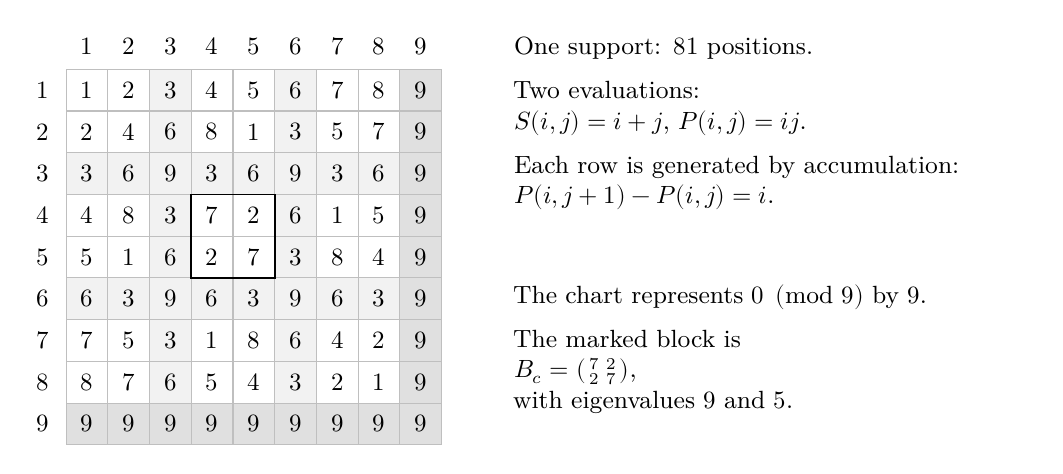
\begin{tikzpicture}[x=.53cm,y=.53cm,font=\small]
\fill[black!5] (1.5,-.5) rectangle (2.5,8.5);
\fill[black!5] (4.5,-.5) rectangle (5.5,8.5);
\fill[black!5] (-.5,2.5) rectangle (8.5,3.5);
\fill[black!5] (-.5,5.5) rectangle (8.5,6.5);
\fill[black!12] (7.5,-.5) rectangle (8.5,8.5);
\fill[black!12] (-.5,-.5) rectangle (8.5,.5);
\foreach \i in {1,...,9}{
 \node at (\i-1,9.05) {\(\i\)};
 \node at (-1.05,9-\i) {\(\i\)};
 \foreach \j in {1,...,9}{
  \pgfmathtruncatemacro{\v}{mod(\i*\j-1,9)+1}
  \node at (\j-1,9-\i) {\(\v\)};
 }
}
\foreach \k in {0,...,9}{
 \draw[black!25] (\k-.5,-.5)--(\k-.5,8.5);
 \draw[black!25] (-.5,\k-.5)--(8.5,\k-.5);
}
\draw[line width=.65pt] (2.5,3.5) rectangle (4.5,5.5);
\node[anchor=west,align=left,text width=6.5cm] at (10,7.2) {One support: \(81\) positions.\\[5pt]Two evaluations:\\ \(S(i,j)=i+j\), \(P(i,j)=ij\).\\[5pt]Each row is generated by accumulation:\\ \(P(i,j+1)-P(i,j)=i\).};
\node[anchor=west,align=left,text width=6.5cm] at (10,1.8) {The chart represents \(0\pmod9\) by \(9\).\\[5pt]The marked block is\\ \(B_c=\left(\begin{smallmatrix}7&2\\2&7\end{smallmatrix}\right)\),\\ with eigenvalues \(9\) and \(5\).};
\end{tikzpicture}
\caption{APP multiplication table in positive representatives. Nonunit rows and columns are distinguished by grey shading; the frame identifies the adjacent diagonal block with equal diagonals. The displayed table is an observable of the arithmetic torus; its representational edges do not constitute an intrinsic topological boundary of the torus.}
\label{fig:app}
\end{figure}


\begin{proposition}[Reconstruction of the evaluations]
The two pairs in \eqref{eq:app-levantada} determine \(i+j\) and \(ij\) exactly. The residues alone determine neither these integer evaluations nor their quotients.
\end{proposition}
\begin{proof}
The first assertion is \eqref{eq:residuo-cociente} applied to each sheet. For the second, \(10=1+9\) and \(19=1+2\cdot9\) have the same residue and different quotients. On the two-dimensional support, the positions \((5,5)\) and \((8,2)\) give the same sum and the same product residue, but products \(25=7+18\) and \(16=7+9\). The residual projection identifies data that the lifted evaluation distinguishes.
\end{proof}

\subsubsection{Cayley graph, toroidal topology, and winding number}

The cardinal translations are given, in row and column coordinates, by
\[
 \nu_N=(-1,0),\quad\nu_E=(0,1),\quad
 \nu_S=(1,0),\quad\nu_O=(0,-1),\qquad T_d(x)=x+\nu_d.
\]
The first coordinate increases southward and the second eastward. The graph
\[
 \mathscr G_9=\operatorname{Cay}(X_9,\{\nu_N,\nu_E,\nu_S,\nu_O\})
\]
is the two-dimensional cyclic lattice: it has eighty-one vertices and four outgoing oriented edges per vertex. It is a Cayley graph for the \emph{additive} structure of the support. Multiplication of residues has zero divisors and does not turn all APP rows into a multiplicative group.

A cardinal word \(w=d_1\cdots d_r\) and an origin \(x_0\) determine
\[
 x_k=x_0+\sum_{j=1}^k\nu_{d_j}\pmod9.
\]
There are \(81\cdot4^r\) oriented paths of length \(r\), including returns and backtracking. When the path closes, its integer displacement prior to reduction defines
\begin{equation}
 \operatorname{wind}(w)=\frac19
 \bigl(\#S(w)-\#N(w),\#E(w)-\#O(w)\bigr)\in\ZZ^2.
\end{equation}
Path reversal changes the sign of this vector. Return to the same residual position therefore does not require the winding to vanish. This is the first instance of a distinction that will recur in phase return: one coordinate may close while another records a nontrivial evolution.

\subsubsection{Transport quotient and cocycle identity}

Let \(s_9:\ZZ/9\ZZ\to D_9\) be the section of positive representatives. The transport quotient associated with additive composition, also called the \emph{carry} in positional arithmetic, is
\[
 c_9(a,b)=\frac{s_9(a)+s_9(b)-s_9(a+b)}9.
\]
The compositional character of this memory is expressed by an exact identity.

\begin{lemma}[Cocycle identity]
For \(a,b,c\in\ZZ/9\ZZ\),
\[
 c_9(a,b)+c_9(a+b,c)=c_9(b,c)+c_9(a,b+c).
\]
\end{lemma}
\begin{proof}
Both sums equal
\[
 \frac{s_9(a)+s_9(b)+s_9(c)-s_9(a+b+c)}9.
\]
Associativity of the sum of lifted representatives requires precisely this additional term when composing in the quotient.
\end{proof}

With positive representatives, this cocycle is not normalized at the identity: \(c_9(0,a)=1\). If \(s_0\) takes representatives in \(\{0,\ldots,8\}\), its normalized carry \(c_0\) satisfies
\[
 c_9(a,b)=c_0(a,b)+\mathbf1_{a=0}+\mathbf1_{b=0}-\mathbf1_{a+b=0}.
\]
The difference is the change of section; it does not alter the cocycle identity. The subsequent decomposition of the calendar into phase and window will use representatives from zero to eight.

The totals of the two evaluations distinguish the visible contribution from that retained in the quotient:
\[
 \sum S=810,\quad\sum P=2025,\quad
 \sum\Sigma=405,\quad\sum\Pi=459,
\]
\[
 \sum q^+=45,\qquad\sum q^\times=174.
\]
It follows that
\begin{equation}
 2025-810=(459-405)+9(174-45)=54+9\cdot129.
 \label{eq:defecto-integrado}
\end{equation}
The sum--product difference is not exhausted by the visible defect \(54\). The identity also preserves the quotient defect \(129\). Suppressing it would change the arithmetic being transported, even if the residual table remained identical.

\subsubsection{Ternary reduction and multiplicative radical}

The ring \(R=\ZZ/9\ZZ\) has unit group \(\{1,2,4,5,7,8\}\) and maximal ideal
\[
 \mathfrak m=(3)=\{0,3,6\},\qquad\mathfrak m^2=0.
\]
Every additive row is a permutation of the nine representatives. A multiplicative row is such a permutation exactly when its index is a unit. Rows three and six contain three repeated values; row nine contains only the representative of the zero class. Thus multiplicative folding already distinguishes the units from the nilpotent sector before any continuous geometry is introduced.

The map \(x\mapsto3x\) has kernel and image both equal to \(\mathfrak m\). It induces an isomorphism of vector spaces over \(\FF_3\),
\[
 R/\mathfrak m\longrightarrow\mathfrak m,\qquad [x]\longmapsto3x,
\]
but not a ring isomorphism. In particular, the visible sequence \(3,6,9\) admits two different readouts: its direct reduction modulo three is \(0,0,0\), whereas extraction of the factor three followed by reduction of its internal coordinate gives \(1,2,0\). This second operation preserves a coordinate of the ideal; it is not the same projection as direct reduction of the original number.

\subsubsection{Latin realization of the additive evaluation}

The distinction between the two evaluations can also be expressed through
operators. Let \((e_r)_{r\in\ZZ/9\ZZ}\) be the orthonormal basis of \(\CC^9\).
The assignment \(v_{ab}=e_{a+b}\) produces an orthonormal basis in each row
and column. The projectors \(P_{ab}=v_{ab}v_{ab}^{*}\) satisfy
\[
 \sum_bP_{ab}=I_9=\sum_aP_{ab},\qquad P_{ab}^2=P_{ab}.
\]
Indeed, each translation \(b\mapsto a+b\) permutes the nine residues.
This yields a rank-one-projector realization of a Latin
square, in the terminology of quantum Latin squares
\cite{mustovicary,delascuevas2023}. This construction starts from the
additive sheet already defined and makes explicit the map to its operator representation.

The multiplicative evaluation preserves different information: for \(a=3\), the
vectors \(e_{3b}\) repeat the residues \(0,3,6\), and
\[
 \sum_{b\in\ZZ/9\ZZ}|e_{3b}\rangle\langle e_{3b}|
 =3\bigl(|e_0\rangle\langle e_0|+|e_3\rangle\langle e_3|
                    +|e_6\rangle\langle e_6|\bigr).
\]
The multiplicity is recorded in the operator and characterizes the multiplicative
radical. Accordingly, the toroidal support, the Latin property, and the
operator resolution of the identity are properties requiring different
definitions. The quantum magic squares studied by
De las Cuevas, Drescher, and Netzer require positive entries and row
and column sums equal to the identity; their theory also distinguishes
dilations with commuting entries\cite{delascuevas2020}. This reference
provides precise terminology for comparing APP realizations.

\subsection{TRIT: orientation and quadratic regimes}

\begin{definition}[Ternary signature and local lift]
The TRIT signature uses the balanced identification
\[
 \FF_3\longrightarrow\TRIT,\qquad 0\mapsto0,\quad1\mapsto+1,\quad2\mapsto-1.
\]
For \(n\in\ZZ\), its lift preserves \(n=r+3c\), where \(r\in\TRIT\) and \(c\in\ZZ\). In a transition of bounded local amplitude, the three states \((0,-1),(0,0),(0,+1)\) may exhibit the same zero residue and different carries.
\end{definition}

The signature does not replace the trajectory. A residual zero does not mean the absence of information about orientation, phase, or quotient. Nor does it by itself introduce a physical quantity. Its function is to distinguish algebraically the transport classes to be realized next.

\subsubsection{Three quadratic regimes and a common exponential}

Once the ternary signature has been obtained, its quadratic realization is defined by
\begin{equation}
 \mathbb A_\tau=\RR[X]/(X^2+\tau),\qquad \tau\in\TRIT.
 \label{eq:algebras-trit}
\end{equation}
If \(J_\tau\) is the class of \(X\), then \(J_\tau^2=-\tau I\). The structure distinguishes the elliptic type \(\tau=+1\), the parabolic type \(\tau=0\), and the hyperbolic type \(\tau=-1\). The real realization does not generate the signature: it expresses the types already produced by oriented reduction.

\begin{proposition}[Exponentiation of the three types]
In each algebra \eqref{eq:algebras-trit},
\begin{equation}
 \exp(tJ_\tau)=C_\tau(t)I+S_\tau(t)J_\tau,
\end{equation}
where
\[
 C_\tau(t)=\sum_{n\ge0}\frac{(-\tau)^nt^{2n}}{(2n)!},\qquad
 S_\tau(t)=\sum_{n\ge0}\frac{(-\tau)^nt^{2n+1}}{(2n+1)!}.
\]
The three realizations are
\[
 \begin{array}{c|c|c}
 \tau&J_\tau^2&\exp(tJ_\tau)\\\hline
 +1&-I&\cos t\,I+\sin t\,J_\tau\\
 0&0&I+tJ_\tau\\
 -1&I&\cosh t\,I+\sinh t\,J_\tau.
 \end{array}
\]
\end{proposition}
\begin{proof}
Separating the even and odd terms of the exponential series and substituting \(J_\tau^{2n}=(-\tau)^nI\) and \(J_\tau^{2n+1}=(-\tau)^nJ_\tau\) gives the formulas. For \(\tau=0\), every term of degree at least two vanishes. In the other two cases, the trigonometric or hyperbolic series are recovered.
\end{proof}

The exponential is common to the three regimes: it is not assigned exclusively to the parabolic branch. The invariants
\[
 C_\tau(t)^2+\tau S_\tau(t)^2=1
\]
follow from \(\exp(tJ_\tau)\exp(-tJ_\tau)=I\). The same algebraic principle preserves unity across realizations that differ in their quadratic type.

In the hyperbolic regime, \(P_\pm=(I\pm J_{-1})/2\) are complementary projectors, and
\[
 \exp(tJ_{-1})=e^tP_++e^{-t}P_-.
\]
Growth and contraction occur jointly in two eigendirections. In the elliptic regime, the parameter describes a rotation; in the parabolic regime, a nilpotent translation. The temporal interpretation adopted by HMT associates \(+1\) with return with memory, \(0\) with the threshold, and \(-1\) with bidirectional opening. This interpretation requires an ordering of the parameterization; it does not add a fourth algebraic type.

% Ampliación acumulativa del TRIT; se inserta antes de la figura de regímenes.
% No sustituye ni elimina el desarrollo precedente.
\subsubsection{Balanced division and composition of lifts}
\label{trit-ampl-div-balanceada}

Ternary reduction makes it possible to express an integer APP evaluation in a
visible coordinate and a prolongation coordinate. Its function is not
merely to abbreviate the writing of an integer: it provides a composition
rule determining how the quotient changes when evaluations are added or
multiplied. The balanced choice also makes explicit
the compatibility of that rule with sign reversal.

\begin{definition}[Balanced ternary coordinates]
\label{trit-ampl-def-coordenadas}
For \(n\in\mathbb Z\), let
\[
 q_3(n)=\left\lfloor\frac{n+1}{3}\right\rfloor,\qquad
 r_3(n)=n-3q_3(n).
\]
The map
\[
 \mathcal B:\mathbb Z\longrightarrow\TRIT\times\mathbb Z,\qquad
 n\longmapsto(r_3(n),q_3(n))
\]
is called the balanced ternary decomposition. Its inverse is
\(\mathcal L(r,c)=r+3c\).
\end{definition}

Indeed, \(r_3(n)\in\{-1,0,+1\}\). If two pairs represent the same integer,
\(r+3c=s+3d\), then \(r-s\) is a multiple of \(3\) lying in the interval
\([-2,2]\); necessarily \(r=s\) and \(c=d\). The representation is therefore
unique. Division can be repeated on \(q_3(n)\), so that each level
preserves the datum needed to reconstruct the preceding one. The quotient is not a
perturbation of the residue: it constitutes its complementary coordinate.

The signature obtained from an evaluation \(F\), with \(F=S\) or \(F=P\) in APP,
is \(r_3\circ F\). When reduction acts on the phase cursor, the same
balanced section produces the classes \(\{1,4,7\}\), \(\{2,5,8\}\), and
\(\{3,6,9\}\), with values \(+1,-1,0\). The TPK selector defined
next uses these classes to determine the operational mode.
Reading an evaluation and selecting a mode thus have the same
ternary reduction, but different domains and functions.

\Needspace{16\baselineskip}
\begin{proposition}[Arithmetic of balanced pairs]
\label{trit-ampl-prop-aritmetica}
Let \(n=r+3c\) and \(m=s+3d\), with \(r,s\in\TRIT\). Define
\[
 \chi(r,s)=\frac{r+s-r_3(r+s)}3.
\]
Integer operations are transported to pairs by
\begin{align}
 (r,c)\boxplus(s,d)
 &=\bigl(r_3(r+s),c+d+\chi(r,s)\bigr),
 \label{trit-ampl-eq-suma}\\
 (r,c)\boxtimes(s,d)
 &=\bigl(rs,rd+sc+3cd\bigr).
 \label{trit-ampl-eq-producto}
\end{align}
The map \(\mathcal L\) preserves both operations.
\end{proposition}
\begin{proof}
The equality \(r+s=r_3(r+s)+3\chi(r,s)\) gives
\[
 n+m=r_3(r+s)+3\bigl(c+d+\chi(r,s)\bigr).
\]
On the other hand,
\[
 nm=rs+3(rd+sc+3cd).
\]
Since the product of two balanced representatives again belongs to
\(\{-1,0,+1\}\), it requires no additional residue reduction. Uniqueness
of the decomposition proves both formulas.
\end{proof}

For example, \(2=(-1)+3\) and \(4=1+3\). Their sum and product are reconstructed
as
\[
 (-1,1)\boxplus(1,1)=(0,2),\qquad
 (-1,1)\boxtimes(1,1)=(-1,3).
\]
The resulting evaluations are \(6\) and \(8\). Adding quotients suffices
in this additive example; the product involves the cross terms
\(rd\), \(sc\), and \(3cd\). The discrepancy between the two operations
also resides in the prolongation coordinate, not only in the residue.

The term \(\chi\) is a cocycle of the balanced section. If
\(r\oplus s=r_3(r+s)\), it satisfies
\[
 \chi(r,s)+\chi(r\oplus s,t)
 =\chi(s,t)+\chi(r,s\oplus t).
\]
Both sides represent the quotient of the same sum of three integers.
This identity guarantees that regrouping the operations does not change the
reconstructed evaluation. At the same time, projection onto the first
component removes that accounting: \(1+1=-1+3\), whereas the residue
readout retains only \(-1\). The discarded information is
determined, in this case, by \(\chi(1,1)=1\).

The relation to modulus \(9\) preserves a second discrete scale.
The map
\[
 \beta:\TRIT\times\mathbb F_3\longrightarrow\mathbb Z/9\mathbb Z,
 \qquad (r,\bar c)\longmapsto r+3c\pmod9
\]
is well-defined and bijective. Changing the representative of \(\bar c\)
adds a multiple of \(9\); conversely, equality of images first fixes
\(r\) by reduction modulo \(3\), and then \(\bar c\). The addition
transported by this bijection contains the term
\(\chi(r,s)\) from \eqref{trit-ampl-eq-suma}, now reduced modulo \(3\).
Thus the two ternary levels are not composed by independent
coordinate addition: normalizing the first level modifies
the second.

In particular, the classes \(3\), \(6\), and \(0\) in
\(\mathbb Z/9\mathbb Z\) have first component \(0\), but second
components \(1\), \(2\), and \(0\), respectively. The distinction already observed
between direct reduction and extraction of the ideal coordinate appears
as a property of \(\beta\). Preserving that coordinate prevents the
zero-residue sector from being artificially turned into a single position.
The modulus \(1000\), used later to organize decimal blocks,
serves another positional-representation function; its quotient is preserved
through the corresponding division. A change of base preserves the integer
when it retains residue and quotient, whereas agreement of residues
in different bases does not by itself identify their transport states.

\Needspace{11\baselineskip}
\subsubsection{Reversal, residue class, and nonvisible coordinates}
\label{trit-ampl-inversion}

Additive inversion lifts unambiguously:
\[
 \mathcal B(-n)=(-r_3(n),-q_3(n)).
\]
In particular, \(3\), \(0\), and \(-3\) have coordinates
\((0,1)\), \((0,0)\), and \((0,-1)\). They share a zero signature but represent
different evaluations. In a transition restricted to a quotient of
maximum magnitude \(1\), they are the three possibilities in the visible fiber over
zero; in a general integer lift, that fiber contains all pairs
\((0,c)\), with \(c\in\mathbb Z\).

The quotient coordinate recovers the evaluated integer, but does not by
itself recover the trajectory that produced it. Two APP paths may share
evaluation, residue, and quotient while differing in orientation, mode sequence, or
winding. Thus the decomposition \(\mathcal B\) is integrated into the
transport state instead of replacing it. The arithmetic memory of a
division and the memory of a trajectory are related coordinates, not
synonyms.

For a signature sequence of length \(n\), oriented reversal is
\[
 C_{\rm rev}(\tau_1,\ldots,\tau_n)
   =(-\tau_n,\ldots,-\tau_1).
\]
Applying it twice restores the sequence. The operation reverses the order of
positions and the sign of each signature; it preserves the length and the
zero positions in reverse order. In the adopted parametrization,
it interchanges return with memory, associated with \(+1\), and bidirectional
opening, associated with \(-1\), while maintaining the threshold \(0\). Transport
of the remaining trajectory data is specified through the
corresponding TPK involution.

This signature reversal must be distinguished from conjugation within a
quadratic algebra. The former may change the type \(\tau\); the latter,
constructed next, acts within the type already fixed. The
distinction prevents attributing to sign reversal an algebraic
equivalence between different regimes.

\subsubsection{Quadratic product, conjugation, and algebraic norm}
\label{trit-ampl-norma}

An element of \(\mathbb A_\tau\) has a unique expression \(aI+bJ_\tau\).
The relation \(J_\tau^2=-\tau I\) determines its product:
\begin{equation}
 (aI+bJ_\tau)(cI+dJ_\tau)
   =(ac-\tau bd)I+(ad+bc)J_\tau.
 \label{trit-ampl-producto-cuadratico}
\end{equation}
This is a real realization of the type already selected. The coordinates
\(a,b\) are not APP residues, and the product
\eqref{trit-ampl-producto-cuadratico} does not replace
\eqref{trit-ampl-eq-producto}; it expresses another operation in the declared
quadratic codomain.

\begin{definition}[Conjugation and algebraic norm]
\label{trit-ampl-def-norma}
Conjugation of type \(\tau\) and its algebraic norm are
\[
 \overline{aI+bJ_\tau}=aI-bJ_\tau,\qquad
 N_\tau(aI+bJ_\tau)=a^2+\tau b^2.
\]
\end{definition}

\begin{proposition}[Multiplicativity and invertibility]
\label{trit-ampl-prop-norma}
For \(z,w\in\mathbb A_\tau\),
\[
 z\bar z=N_\tau(z)I,\qquad
 N_\tau(zw)=N_\tau(z)N_\tau(w).
\]
Moreover, \(z\) is invertible if and only if \(N_\tau(z)\ne0\), in which case
\[
 z^{-1}=\frac{\bar z}{N_\tau(z)}.
\]
\end{proposition}
\begin{proof}
The product of \(aI+bJ_\tau\) and \(aI-bJ_\tau\) is
\((a^2+\tau b^2)I\). Conjugation is multiplicative and the algebra is
commutative, so
\((zw)\overline{zw}=(z\bar z)(w\bar w)\). If the norm is nonzero, the
stated formula provides the inverse. Conversely, if \(zw=I\),
multiplicativity implies \(N_\tau(z)N_\tau(w)=1\).
\end{proof}

The quadratic form \(N_\tau\) is positive definite only in the elliptic type.
For \(\tau=0\), it equals \(a^2\), and the element \(J_0\) is nonzero although its
square and norm are zero. For \(\tau=-1\), it equals \(a^2-b^2\); the
nonzero elements \(I+J_{-1}\) and \(I-J_{-1}\) have zero norm and their
product vanishes. The algebraic norm here is a multiplicative quadratic
form: it does not presuppose a positive vector-space norm.

All three types can be faithfully realized by
\[
 aI+bJ_\tau\longmapsto
 \begin{pmatrix}a&-\tau b\\b&a\end{pmatrix}.
\]
The determinant of this matrix is \(N_\tau(aI+bJ_\tau)\). Thus
the complex structure, the dual-number structure, and the split-real
structure are represented by the same matrix expression.
Each preserves its law and zero divisors. The form of signature
\((1,1)\) in the last case has a Lorentzian interpretation in dimension
\(1+1\); identifying a physical metric additionally requires a specific space,
field, and transport rule.

\subsubsection{Multiplicative conservation and composition of evolutions}
\label{trit-ampl-evoluciones}

The exponential already obtained belongs to the set of norm-one elements:
\[
 N_\tau\bigl(\exp(tJ_\tau)\bigr)=1.
\]
This conservation persists under composition of parameters. Indeed, all
factors are functions of the same generator, and
\[
 \exp(tJ_\tau)\exp(sJ_\tau)=\exp((t+s)J_\tau).
\]
Comparing the two components yields the addition laws
\begin{align}
 C_\tau(t+s)&=C_\tau(t)C_\tau(s)-\tau S_\tau(t)S_\tau(s),\\
 S_\tau(t+s)&=S_\tau(t)C_\tau(s)+C_\tau(t)S_\tau(s).
\end{align}
Conjugation changes \(t\) to \(-t\) and coincides with inversion within
this subgroup. It does not change \(\tau\): it reverses an evolution in the chosen
regime.

In the elliptic type, the preserved form is \(a^2+b^2\), and the exponential
trajectory traverses the norm-one circle. In the hyperbolic type, the
eigen-coordinates are \(u=a+b\), \(v=a-b\), with \(uv=N_{-1}(z)\).
The exponential gives
\[
 (u,v)=(e^t,e^{-t}),\qquad uv=1.
\]
Growth of one coordinate is accompanied by contraction of the other.
Conservation expresses a relation between the two coordinates; it does not assert
that each remains constant.

In the parabolic type,
\[
 (I+tJ_0)(I+sJ_0)=I+(t+s)J_0,\qquad
 (I+tJ_0)^{-1}=I-tJ_0.
\]
Evolution does not stop because \(J_0^2=0\). Nilpotence eliminates
terms of order at least two, but preserves the linear term
transporting the parameter. The visible symbol \(0\), the
zero element of the algebra, and the nonzero generator \(J_0\) are distinct. This distinction
is necessary to describe the threshold without identifying it with the absence of
a state or dynamics.

\begin{proposition}[Composition of affine coordinates]
\label{trit-ampl-prop-pendientes}
In the chart where the scalar component is nonzero, represent a
direction by \(I+uJ_\tau\). If \(1-\tau uv\ne0\), the direction of its
product with \(I+vJ_\tau\) has coordinate
\[
 u\star_\tau v=\frac{u+v}{1-\tau uv}.
\]
\end{proposition}
\begin{proof}
We have
\[
 (I+uJ_\tau)(I+vJ_\tau)
   =(1-\tau uv)I+(u+v)J_\tau.
\]
Dividing by the scalar component gives the stated expression.
\end{proof}

The affine chart preserves the ratio between components, not the scalar factor
divided out. When \(1-\tau uv=0\), the product must be examined before
changing charts: it may have a defined direction with zero scalar
component, or be the zero element in the presence of zero divisors. The composition
law still belongs to the complete algebra; a coordinate singularity
does not automatically amount to a singularity of the object.
This formula will reappear in the elliptic regional readout. Its use requires
retaining the denominator and, where applicable, the normalization factor.

\subsubsection{Transport of type and subsequent realizations}
\label{trit-ampl-puentes}

The algebras \(\mathbb A_{+1}\), \(\mathbb A_0\), and
\(\mathbb A_{-1}\) are not isomorphic as unital real algebras.
The first is a field; the second contains a nonzero nilpotent; the
third has nontrivial idempotents and is isomorphic to
\(\mathbb R\times\mathbb R\). Thus the signature change organizing a
route cannot be interpreted as an undifferentiated isomorphism between the
three realizations. The TPK preserves the regime index, domains, and
effective operator acting at each transition.

In the electron chapter, the pair of projections of the APP sheets
produces a normalized commutator whose square is \(-I\). The same block
contains an involution squaring to \(I\) and two nilpotent directions. The
joint realization will be proved on that concrete pair of projections;
the preceding classification explains why the three quadratic relations
can appear in the same matrix algebra without being identified with one another.

In the exceptional prolongation, the Paley matrix reduced modulo \(3\)
satisfies \(A_W^2=-I_6\). The relation equips the ternary space with a
structure of dimension \(3\) over \(\mathbb F_9\). Its link to a real
operator root is expressed through the integral presentation
\[
 \mathbb Z[u]/(u^2+1).
\]
Base changes to \(\mathbb F_3\) and \(\mathbb R\) produce
representations of the same relation. Each preserves its characteristic,
dimension, and incidence information. The development of the
respective operators establishes the link, not equality of their
cardinalities.

Preservation of norm one therefore describes the quadratic
realizations of evolutions. Preservation of quotients, orientation, and
trajectory belongs to the transported arithmetic state. Both properties
enter the construction, with different functions: one determines the
identities of the representations; the other makes it possible to compose, reconstruct, and
prolong the operations giving rise to them.


\begin{figure}[htbp]
\centering
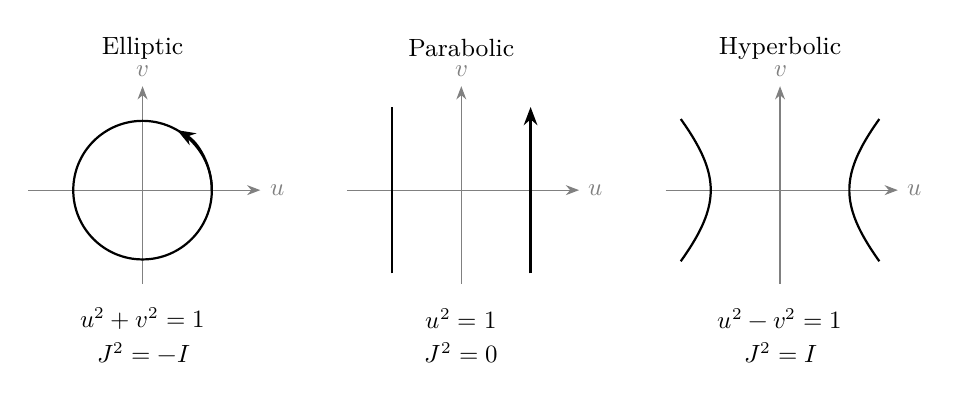
\begin{tikzpicture}[scale=.88,>=Stealth,font=\small]
\foreach \c/\titulo in {0/{Elliptic},4.6/{Parabolic},9.2/{Hyperbolic}}{
\begin{scope}[xshift=\c cm]
\draw[->,gray] (-1.65,0)--(1.7,0) node[right] {\(u\)};
\draw[->,gray] (0,-1.35)--(0,1.5) node[above] {\(v\)};
\node at (0,2.05) {\titulo};
\end{scope}}
\draw[thick] (0,0) circle[radius=1];
\draw[->,thick] (1,0) arc[start angle=0,end angle=60,radius=1];
\node at (0,-1.85) {\(u^2+v^2=1\)};
\node at (0,-2.35) {\(J^2=-I\)};
\draw[thick] (3.6,-1.2)--(3.6,1.2);
\draw[->,thick] (5.6,-1.2)--(5.6,1.2);
\node at (4.6,-1.85) {\(u^2=1\)};
\node at (4.6,-2.35) {\(J^2=0\)};
\draw[thick,domain=-.9:.9,samples=50] plot ({9.2+cosh(\x)},{sinh(\x)});
\draw[thick,domain=-.9:.9,samples=50] plot ({9.2-cosh(\x)},{sinh(\x)});
\node at (9.2,-1.85) {\(u^2-v^2=1\)};
\node at (9.2,-2.35) {\(J^2=I\)};
\end{tikzpicture}
\caption{Quadratic realizations of TRIT. For
\(J_\tau=\left(\begin{smallmatrix}0&-\tau\\1&0\end{smallmatrix}\right)\),
the exponential preserves \(u^2+\tau v^2\). The parabolic degeneration
preserves \(u\) and transports \(v\) linearly. The three diagrams represent
orbits of quadratic forms; their geometric type corresponds to the
algebraic relation of the generator.}
\label{fig:trit-regimenes}
\end{figure}


\newpage
\subsection{TPK: topological phase kernel}

The dynamics uses the phase selector
\[
 M_{\rm ph}(r)=
 \begin{cases}
 +1,&r\in\{1,4,7\},\\
 -1,&r\in\{2,5,8\},\\
 0,&r\in\{3,6,9\}.
 \end{cases}
\]
Its value determines which evaluation acts. Cardinal transport displaces the corresponding cursor; the record preserves the previous value, the new quotient, the orientation, and the transition. Selection and transport are therefore distinct functions: a ternary sign is not a displacement on the torus.

We denote by \(\widehat X\) the space of arithmetic states with trajectory memory. An element contains the positions and directions of the two cursors, the active mode, the TRIT signature, the phase, the residues and quotients of both evaluations, the carries, the constructed prefix, and the boundary data. When a refinement cylinder is introduced, it forms part of the state. This notation avoids replacing the object with a reduced version that retains only the visible symbol.

\begin{definition}[TPK update]
Let \(\mathsf{Sel}_t\) be mode selection by \(M_{\rm ph}\), \(\mathsf{Tra}_t\) the lifted cardinal transport, and \(\mathsf{Mem}_t\) the record update. The transition is
\begin{equation}
 \mathcal U_t=\mathsf{Mem}_t\circ\mathsf{Tra}_t\circ\mathsf{Sel}_t.
 \label{eq:actualizacion}
\end{equation}
Each application preserves the fields it does not modify and updates the remaining fields through Euclidean division and trajectory concatenation.
\end{definition}

The notation \eqref{eq:actualizacion} expresses the order of composition; it does not replace the effective rules. The next section fully specifies its finite two-cursor realization. Prolongation will then be obtained not by erasing its memory and repeating the first emission, but by transporting the prefixes and their compatible boundaries. Thus APP supplies the evaluations, TRIT distinguishes their regimes, and TPK composes their evolution.

% Recuperación expositiva desde los propietarios del núcleo TPK.
% La procedencia y el control de conservación se documentan en technical/TPK_INTEGRACION.md.
% Este archivo amplía la sección TPK; no sustituye extension.tex ni generacion.tex.

\subsubsection{Dynamic state, observables, and dependence of the operations}
\label{tpk-int:estado}

The Topological Phase Kernel organizes the evolution of the two APP sheets
with the orientation determined by TRIT. Its definition comprises the state
on which it acts, the transition rules, and the relations that make
prolongations compatible. Equation \eqref{eq:actualizacion} acquires
operational content by specifying which coordinates each of its
factors receives and modifies. Position belongs to the toroidal support; phase
belongs to the calendar; orientation determines transport;
quotients record the arithmetic evaluation before its reduction.
These coordinates are related through the transition and preserve different
mathematical functions.

The observable projection of a state is
\begin{equation}
 q=(x_+,d_+,x_\times,d_\times,\theta)
 \in\mathcal Q_{\rm obs}
 :=(X_9\times\mathcal D)^2\times\Theta_{108},
 \qquad \mathcal D=\{N,E,S,O\},\quad
 \Theta_{108}=\ZZ/108\ZZ.
 \label{tpk-int:qobs}
\end{equation}
The subscripts distinguish the additive and multiplicative cursors. The
fibers of complete states over \(q\) preserve the ordered trajectory, the integer
evaluations of both sheets, their residues and quotients, and the
orientation and boundary registers. A precision prolongation adds the
prefix and the compatible cylinder. Thus two states with the same
projection \(q\) may preserve different registers.

The dependence of the operations has three levels. At the local level,
the selector activates a sheet, transport modifies its position, and the
update calculates the new arithmetic coordinates. At the trajectory
level, these transitions are composed and preserve the registers of
earlier steps. At the refinement level, extension
relations determine which continuation preserves the prefix, signature, and
boundary of its predecessor. The finite calendar describes the phase of these
operations; holonomy describes their composition on the history.

\subsubsection{Trit selection and lifted cardinal transport}
\label{tpk-int:seleccion}

Let \(\bar\theta\in\{0,\ldots,107\}\) be the calendar representative.
The operational phase and dodecaphasic sector are
\begin{equation}
 r(\theta)=1+(\bar\theta\bmod9),\qquad
 \beta(\theta)=\left[\left\lfloor\frac{\bar\theta}{9}\right\rfloor\right]_{12}.
 \label{tpk-int:fase}
\end{equation}
The selector already defined can be written \(\varepsilon_9=M_{\rm ph}\).
Its value vector, in the ordered chart of \(D_9\), is
\[
 m_{\rm ph}=(1,-1,0,1,-1,0,1,-1,0).
\]
The function \(M_{\rm ph}:D_9\to\TRIT\) and this vector are two
presentations of the same selector, with their respective domains.

Define the activation indicators
\[
 a_+(\theta)=\mathbf1_{\{1,4,7\}}(r(\theta)),\qquad
 a_\times(\theta)=\mathbf1_{\{2,5,8\}}(r(\theta)).
\]
Cursor transport is then
\begin{equation}
 x_+'=x_++a_+(\theta)\nu_{d_+},\qquad
 x_\times'=x_\times+a_\times(\theta)\nu_{d_\times}
 \quad\text{in }X_9.
 \label{tpk-int:cursores}
\end{equation}
In phases \(3,6,9\), both positions remain unchanged; the neutral event
is part of the chronology and its register. Cardinal directions
determine the vectors \(\nu_d\), while the phase signature determines
which of those vectors is applied.

The integer lift preserves boundary crossing. If
\(s:X_9\to D_9^2\) chooses positive representatives and
\(x'=x+a\nu_d\), with \(a\in\{0,1\}\), define
\begin{equation}
 b_d(x,a)=\frac{s(x)+a\nu_d-s(x')}{9}\in\ZZ^2.
 \label{tpk-int:borde}
\end{equation}
Divisibility by \(9\) follows from equality in \(X_9\).
If \(z\in\ZZ^2\) records earlier crossings, the update is
\(z'=z+b_d(x,a)\). Thus
\[
 s(x')+9z'=s(x)+9z+a\nu_d.
\]
The integer transport datum remains reconstructible after reducing
the position on the torus.

\begin{proposition}[Preservation of lifted displacement]
\label{tpk-int:prop-desplazamiento}
For a cardinal trajectory of \(n\) steps, whose activation
indicators are \(a_t\), we have
\[
 s(x_n)+9z_n=s(x_0)+9z_0+
 \sum_{t=0}^{n-1}a_t\nu_{d_t}.
\]
The same equality is preserved when two compatible trajectories are concatenated.
\end{proposition}
\begin{proof}
The one-step identity is \eqref{tpk-int:borde}. Summing it over the
\(n\) steps cancels the intermediate coordinates. Dividing the summation
interval into two segments produces exactly the concatenation law. For a
closed trajectory, the difference \(z_n-z_0\) is the winding
number defined earlier.
\end{proof}

The same principle governs APP evaluations. If a sheet takes the
integer value \(N_t\), its register simultaneously preserves
\(N_t=R_t+9q_t\). The difference between two steps satisfies
\[
 N_{t+1}-N_t=(R_{t+1}-R_t)+9(q_{t+1}-q_t).
\]
Spatial-crossing memory \(z_t\) and the arithmetic quotient \(q_t\)
have different definitions; their joint preservation maintains the
geometric and arithmetic provenance of each transition.

\subsubsection{Two-cursor chronology and composite returns}
\label{tpk-int:cronologia}

The cardinal involution \(\jmath\) interchanges \(N\) with \(S\) and
\(E\) with \(O\). After \eqref{tpk-int:cursores} is applied, both
directions are reversed whenever a block of \(27\) steps ends.
Writing
\[
 h(\theta)=\mathbf1_{\{0,27,54,81\}}
             ((\bar\theta+1)\bmod108),
\]
the complete rule on the observable projection is
\begin{equation}
 F_{\rm obs}(q)=
 \bigl(x_+',\jmath^{h(\theta)}d_+,
       x_\times',\jmath^{h(\theta)}d_\times,
       \theta+1\bigr).
 \label{tpk-int:fobs}
\end{equation}
The readout forming the emission uses the positions before
transport, according to the explicit recurrence in
Section~\ref{sec:extension}. The observable update and emission
are therefore composed in a fixed order.

\begin{proposition}[Reversibility and period of the observable calendar]
\label{tpk-int:periodo}
The map \(F_{\rm obs}\) is a permutation of
\(\mathcal Q_{\rm obs}\) and satisfies \(F_{\rm obs}^{108}=I\).
In a block of \(54\) steps, positions and directions are restored;
the coordinate in \(\Theta_{108}\) advances by \(54\).
\end{proposition}
\begin{proof}
Given the final state, one first recovers the previous phase by subtracting one
in \(\Theta_{108}\). That phase determines whether the
directions were reversed and which cursor moved. Applying the corresponding involution
and subtracting the cardinal vector uniquely recovers the initial state.

Each interval of \(27\) steps contains nine activations of each
cursor. The next block preserves the activations and reverses the
directions, so the integer displacements cancel in
\(54\) steps. The rule has period \(54\) in its position
and orientation increments; the same cancellation holds for any calendar
origin. After \(108\) steps, \(\theta\) is also restored.
\end{proof}

We reserve
\[
 \mathcal K_{27}=F_{\rm obs}^{27}:
 \mathcal Q_{\rm obs}\longrightarrow\mathcal Q_{\rm obs}
\]
for the iterate of \(27\) transitions. Its fourth iterate is the
identity on the observable state defined in \eqref{tpk-int:qobs}.
Projecting history onto the calendar makes this finite
check possible. The trajectory register, its evaluations, and
new prefixes are preserved in the dynamic state on which
\(\mathcal U_t\) acts; the observable equality does not reset them.

\subsubsection{Affine memory transport and state composition}
\label{tpk-int:memoria}

The observable projection admits fibers of arithmetic and geometric data.
Over a configuration \(q\), write a state in the form
\[
 x=(q,o,h,c,\sigma,C,b,\lambda).
\]
Here \(o\) preserves orientation and sheet; \(h\), residues
and quotients; \(c\), additive transport memory; \(\sigma\),
the boundary signature; \(C\), the precision cylinder; \(b\), its
boundary label; and \(\lambda\), the recorded trajectory. The
signature is determined by a map
\[
 \operatorname{Sig}_q:
 \mathsf H_q\times\mathsf C_q\times\mathsf{Hist}_q
 \longrightarrow\mathsf S_q,
 \qquad \sigma=\operatorname{Sig}_q(h,c,\lambda).
\]
The symbols \(\mathsf H_q,\mathsf C_q,\mathsf{Hist}_q\) and
\(\mathsf S_q\) denote, respectively, the sets of
residue--quotient data, the abelian group of transport memory, the
recorded trajectories, and the boundary signatures.
Realizations of this signature are specified with their components in
the regional and terminal constructions. This dependence prevents
treating the signature as a free parameter once the data producing it are fixed.

The elementary residue-and-quotient chart is explicit. For
\(n\in\ZZ\), let
\[
 r=1+((n-1)\bmod9),\qquad u=\frac{n-r}{9}.
\]
Then \(n=r+9u\), with \(r\in D_9\) and \(u\in\ZZ\).
Uniqueness follows because two representatives in \(D_9\) congruent
modulo \(9\) are equal. This chart provides local integer
reconstruction. The precision towers additionally incorporate truncation
maps and the cylinders developed in
\ref{sec:extension} and \ref{sec:generacion}.

Let \(\gamma:q\to q'\) be an observable trajectory. Fiber
transport is expressed by maps
\[
 \mathsf H(\gamma):\mathsf H_q\to\mathsf H_{q'},\qquad
 \mathsf C(\gamma):\mathsf C_q\to\mathsf C_{q'},\qquad
 \mathsf{Hist}(\gamma):\mathsf{Hist}_q\to\mathsf{Hist}_{q'}.
\]
The maps respect identities and composition, and
\(\mathsf C(\gamma)\) is an abelian-group homomorphism.
The increment \(k_{\rm tr}(\gamma)\in\mathsf C_{q'}\) satisfies
\begin{equation}
 \begin{split}
 k_{\rm tr}(\operatorname{id}_q)&=0,\\
 k_{\rm tr}(\gamma_2\circ\gamma_1)
 &=k_{\rm tr}(\gamma_2)+
   \mathsf C(\gamma_2)k_{\rm tr}(\gamma_1).
 \end{split}
 \label{tpk-int:cociclo}
\end{equation}
The symbol \(k_{\rm tr}\) here denotes the transport cocycle;
the rational coordinate \(\kappa\) of the register \(K\) retains
its notation in the chapter on dodecaphasic closure.

The transportable coordinates are updated by
\begin{equation}
 \begin{aligned}
 h'&=\mathsf H(\gamma)h,&
 c'&=\mathsf C(\gamma)c+k_{\rm tr}(\gamma),\\
 \lambda'&=\gamma\circ\lambda,&
 \sigma'&=\operatorname{Sig}_{q'}(h',c',\lambda').
 \end{aligned}
 \label{tpk-int:accion-memoria}
\end{equation}
The second equation is an affine action: the linear term transports
the previous memory, and the cocycle adds the increment produced by the
trajectory. In the spatial-crossing realization for each cursor separately,
\(\mathsf C(\gamma)=I\), and \(k_{\rm tr}(\gamma)\) is the sum
of the vectors in \eqref{tpk-int:borde}. This concrete instance
links the abstract law to the cardinal operations already defined.

\begin{proposition}[Compatibility of the update with concatenation]
\label{tpk-int:composicion-memoria}
Updating \eqref{tpk-int:accion-memoria} by
\(\gamma_1\), followed by updating by \(\gamma_2\),
coincides with updating by \(\gamma_2\circ\gamma_1\).
\end{proposition}
\begin{proof}
For the affine coordinate, two updates give
\[
 c''=\mathsf C(\gamma_2)\mathsf C(\gamma_1)c
       +\mathsf C(\gamma_2)k_{\rm tr}(\gamma_1)
       +k_{\rm tr}(\gamma_2).
\]
Functoriality of \(\mathsf C\) and
\eqref{tpk-int:cociclo} turn this expression into
\(\mathsf C(\gamma_2\circ\gamma_1)c+
k_{\rm tr}(\gamma_2\circ\gamma_1)\).
The assertion for \(h\) follows from composition of
\(\mathsf H\), and that for \(\lambda\) from associativity of
trajectories. The final signature agrees because it is evaluated on the same
three reconstructed coordinates.
\end{proof}

The cylinder and its boundary complete this law through the relations
\(\operatorname{Ext}_\gamma\), defined in
\ref{tpk-int:bidireccionalidad}. Their elements determine which of
the preceding updates preserve an admissible prolongation.
States, together with the triples \((\gamma,x,x')\) admitted by
these relations, form a category over observable trajectories:
\[
 (\gamma_2,x',x'')\circ(\gamma_1,x,x')
     =(\gamma_2\circ\gamma_1,x,x'').
\]
The identity of \(x\) is \((\operatorname{id}_q,x,x)\).
Composition preserves both arithmetic transport and boundary
prolongability. This is the structure in which returns with
memory and successive refinements take place.

\subsubsection{Dodecaphasic register, phase, and accumulated memory}
\label{tpk-int:dodecafase}

The \(108\) transitions are distributed over the ordered windows
\[
 E_m=\{9m-8,\ldots,9m\},\qquad 1\leq m\leq12.
\]
The register preserves the phase origin, orientation, and data
produced during each window. Its map is
\[
 \mathcal R_{12}(x)=
 \bigl((E_m,\tau_m,\sigma_m,\kappa_m,\Lambda_m)\bigr)_{m=1}^{12},
\]
where \(\tau_m\) is the window subroute, \(\sigma_m\) its
orientation, \(\kappa_m\) the integer boundary increment, and
\(\Lambda_m\) the local incidence register. We adopt the chart
to be developed in \ref{subsec:k-registro-integral}; its window
indices correspond to \(m=\beta+1\).
The domain comprises compatible TPK
histories, and the codomain their oriented temporal registers. The
composition of segments and their increments is governed by
\eqref{tpk-int:accion-memoria}. The group \(C_{12}\), by
contrast, describes translation of the window index; \(\Theta_{108}\) preserves
the step calendar. This distinction makes it possible to specify what is transformed
and what is observed when a cycle is completed.

In coordinates \(\theta=9b+r\), with \(0\leq r<9\), advancement
by \(9\) steps preserves \(r\) and increases \(b\) by one.
Phase addition introduces the quotient
\[
 c_0(r,r')=\left\lfloor\frac{r+r'}9\right\rfloor,
\]
whose cocycle identity ensures associativity of composition.
The finite calendar retains \([b]_{12}\); a winding
register retains \(b\in\ZZ\), or \(b\in\mathbb N_0\) for
a history with fixed origin. Section~\ref{sec:extension} proves
the nonsplit exact sequence \eqref{eq:extension108}. Its role is to
describe the relation between these coordinates before they are used in
constructing the signed state.

The signed register receives phase and memory data through the
composition developed in Section~\ref{sec:k-registro}:
\begin{equation}
 R_{\rm sgn}=\Pi_H\circ\mathcal E_{108}^{90,120}
                         \circ\mathcal R_{12}.
 \label{tpk-int:registro-causal}
\end{equation}
Its domain is the terminal state with memory; its output belongs to
\(\ZZ^{12}\). The reversible transformation between that signed state
and \(K\), as well as the rational readout of \(K\), are proved in
the corresponding chapter. The registration operations precede
those transformations. Reconstructing a register from its
cyclic differences verifies recoverability; its dynamic provenance
must be preserved through the events that produced it.

For the encoded trace \((d_t)\) preserved by the register, the
event readout counts the codes \(\{2,4,6,8\}\) in each
window with orientation
\((+,+,+,-,-,-,+,+,+,-,-,-)\). These codes and the
cardinal symbols of \(\mathcal D\) are different coordinates of the
register. Chapter~\ref{sec:k-registro} develops this readout,
the integral decomposition \(1+5+6\), the congruences
characterizing its image, and its exact inverse. The inversion proof
establishes which data that chart preserves; the definition of
\(\mathcal R_{12}\) specifies the oriented history on which
it acts.

\subsubsection{Phase incidence and internal construction of the channels}
\label{tpk-int:incidencia}

The selector determines three subsets of \(D_9\):
\[
 H_+=\{1,4,7\},\qquad H_-=\{2,5,8\},\qquad H_0=\{3,6,9\}.
\]
Let \(H_{\rm act}=H_+\sqcup H_-\) be the set of active phases, and
let \(O_{\rm ph}=D_9\setminus\{9\}\) be the chart preceding the marked
return. Denote by \(P_2(H_{\rm act})\) the set of
unordered pairs of active phases. Internal incidence is given by
\begin{equation}
 \mathcal F^{\rm ph}_6=H_{\rm act}\times P_2(H_{\rm act}),\qquad
 \mathcal F^{\rm ph}_8=O_{\rm ph}\times P_2(H_{\rm act}),\qquad
 \Theta_{\rm ph}=D_9\times P_2(H_{\rm act}).
 \label{tpk-int:fases90120}
\end{equation}
The indices describe the number of positions in the first component.
The construction uses the phases and calendar origin already fixed;
subsequent exceptional realizations will transport these
incidences to their own domains.

\begin{proposition}[Cardinalities and oriented phase incidence]
\label{tpk-int:cardinales}
The sets in \eqref{tpk-int:fases90120} have cardinalities
\(90,120,135\), respectively. If
\[
 \partial_{\rm ph}=\Theta_{\rm ph}\times\{-1,+1\},\qquad
 E_{\rm ph}=\partial_{\rm ph}\sqcup\{\infty\},\qquad
 L_{\rm ph}=H_0\times P_2(H_{\rm act}),
\]
then
\[
 |\partial_{\rm ph}|=270,\quad |E_{\rm ph}|=271,\quad
 |L_{\rm ph}|=45,\quad
 |\partial_{\rm ph}\sqcup L_{\rm ph}|=315.
\]
Simultaneously translating the phase origin and marked return preserves
all these cardinalities and their inclusions.
\end{proposition}
\begin{proof}
There are six active phases, so
\(|P_2(H_{\rm act})|=\binom62=15\). Products by
\(6,8,9\) give \(90,120,135\). Orientation doubles \(135\);
the return mark adds one element; the three neutral phases give
\(3\cdot15=45\). A calendar translation transports each
factor by a bijection and carries the marked point to its image.
Products and disjoint unions thus preserve incidence.
\end{proof}

The cardinality \(271\) here has a realization through phase
incidence. The cubic completion in Section~\ref{sec:extension} has
its own construction of the shell \(1000-729\). The correspondence
between both realizations must preserve the maps and markings that
identify them, in addition to cardinality. Likewise, the selector
\(\varepsilon_9\), the incidence \((90,120)\), and the extractor
\(\mathcal E_{108}^{90,120}\) preserve the domains and operations
just distinguished.

\subsubsection{Trajectory reversal and conjugate prolongations}
\label{tpk-int:bidireccionalidad}

Bidirectionality begins with an operation on trajectories, before
scalar values are assigned to them. For
\(\gamma=(x_0;d_1,\ldots,d_n)\), with endpoint \(x_n\), define
\[
 \operatorname{rev}\gamma
   =(x_n;\jmath d_n,\ldots,\jmath d_1).
\]
The origin of the reverse trajectory is the endpoint of the original.
Composition satisfies
\[
 \operatorname{rev}^2\gamma=\gamma,\qquad
 \operatorname{rev}(\gamma_2\circ\gamma_1)
   =\operatorname{rev}\gamma_1\circ\operatorname{rev}\gamma_2,
\]
and the integer displacement changes sign. These identities are obtained
by reversing the order of steps and replacing each cardinal vector by
its opposite. For a loop it follows that
\(\operatorname{wind}(\operatorname{rev}\gamma)
=-\operatorname{wind}(\gamma)\).

On registers, reversal also requires transporting the order
of their components and the orientation of their events. Route
reversal and signature conjugation are distinguishable operations: their
composition is specified when applied to a concrete register. In
particular, the regional involution interchanging the closure
and propagation components preserves the self-scaling axis; its formula is
presented in Section~\ref{mono-ampl:regiones}. This regional operation
acts on a different domain from reversal of a cardinal trajectory.

Extensions over a route \(r:q\to q'\) are expressed through
relations between fibers of compatible states. If \(\mathcal F_q\)
denotes the fiber of complete states over \(q\), one requires
\[
 \operatorname{Ext}_r\subseteq\mathcal F_q\times\mathcal F_{q'},
 \qquad \Delta_{\mathcal F_q}\subseteq
        \operatorname{Ext}_{\operatorname{id}_q},
\]
\[
 \operatorname{Ext}_{r_2}\circ\operatorname{Ext}_{r_1}
       \subseteq\operatorname{Ext}_{r_2\circ r_1}.
\]
Their composition preserves the evaluations of both sheets, orientation,
quotients, prefix, and boundary. Route reversal does not
by itself imply that every extension relation is a bijection.
Conjugate prolongation is defined on the domain where transport of
these data satisfies the corresponding compatibilities.

\subsubsection{Nonadic holonomy and continuity of refinement}
\label{tpk-int:holonomia}

One phase winding composes transitions on the state with memory:
\begin{equation}
 \Gamma_{9,k}=\mathcal U_{k+8}\circ\cdots\circ\mathcal U_k.
 \label{tpk-int:gamma}
\end{equation}
On an individualized history, this functional composition realizes
the holonomy relation; on the complete domain one retains
\(\Gamma_{9,k}\subseteq\widehat X_k\times\widehat X_{k+9}\),
with the admissible prolongations developed below.
The cyclic base has nine phases, whereas
the fiber preserves the trajectory, quotients, and boundary.
Monodromy is the action of one winding of that base on the fibers;
holonomy \(\Gamma_{9,k}\) expresses its realization by the effective
TPK transitions.

If \(g\) observes the phase and \(M\) the number of retained windings,
\[
 g(\Gamma_{9,k}x)=g(x),\qquad M(\Gamma_{9,k}x)=M(x)+1.
\]
The first identity expresses phase closure, and the second identifies
the new temporal depth. Coinductive prolongation additionally preserves
its cylinders and prefixes. Restrictions between depths
compose an inverse system; a compatible section gathers its
predecessors without replacing them by the last observation. The development
of this arithmetic of histories and its unit occupies
\ref{hist:seccion}--\ref{hist:doble-varianza}; the construction of
regions and their readouts is carried out in Section~\ref{sec:generacion}.

Phase transfer on emissions already constructed has a different
domain. Let \(\mathcal A_+\) and \(\mathcal A_\times\) be the
alphabets of additive and multiplicative signatures, with cardinalities \(18\)
and \(26\). Their product identifies the catalogue \(\mathcal U_6\).
For \(f:\mathcal A_+\times\mathcal A_\times\to\RR\),
the sheet averages are
\[
 (E_+f)(s,e)=\frac1{18}\sum_{s'\in\mathcal A_+}f(s',e),\qquad
 (E_\times f)(s,e)=\frac1{26}\sum_{e'\in\mathcal A_\times}f(s,e').
\]
These emissions and their cardinalities are constructed through
the recurrence in Section~\ref{sec:extension}. Once they have been obtained,
the transfer operator is defined on
\(\mathcal U_6\times C_9\) by
\[
 P_+=E_+,\quad P_-=E_\times,\quad P_0=I,\qquad
 \mathcal K_{\rm ph}((u,r),(v,r+1))=P_{M_{\rm ph}(r)}(u,v),
\]
with zero weight for the remaining phase transitions. The index
\(r\) uses the positive representative of the cyclic class.
The phase order \((+1,-1,0)^3\) then produces the renewal
\[
 \mathcal K_{\rm ph}^{9}\big|_r=E_+E_\times.
\]
Indeed, both averages are idempotent, commute, and average different
factors; their composition assigns weight \(1/(18\cdot26)=1/468\)
to each emission. This equality characterizes a subsequent transfer
observable. Transport of histories remains given by
\eqref{tpk-int:gamma}, with its memory and boundary.

The resulting hierarchy establishes the role of the following chapters.
Finite emission constructs the domain and regions; extension
relations preserve their prefixes; the nonadic connection prolongs them; the
dodecaphasic register determines the data entering \(K\) and
the closure of \(\alpha\). The numerical and incidence
realizations receive that prior structure. This order makes it possible to present
each consequence in its chapter while preserving, from the formal kernel,
the objects that make it possible.


\subsection{Accumulated memory and transport resolvents}
\label{subsec:memoria-resolvente}

Calendar return does not eliminate the increments produced during
the traversal. To express this difference in operator terms, an
accumulative register of trajectory events is constructed first, followed by its
generating series. Memory variables will be reduced on
that transport, while preserving the source and output readout as well.

\subsubsection{Oriented events and register update}

Let \((d_t)\) be the sequence of integer direction codes preserved
by a TPK trajectory. The code \(d_t\) and the cursor's cardinal
direction are different coordinates; no identification
between their alphabets is assumed. Number the windows from zero:
\[
 I_m=\{9m+1,\ldots,9m+9\},\qquad m\geq0.
\]
In the first cycle, \(I_m\) is window \(E_{m+1}\) of the dodecaphasic
register. Its orientation is
\(\sigma=(1,1,1,-1,-1,-1,1,1,1,-1,-1,-1)\).
For a prolonged history, \(\sigma_m\in\{-1,1\}\) is the sign
preserved in the corresponding window. The signed event is
\begin{equation}
 a_m=\sigma_m\sum_{t\in I_m}
       \mathbf1_{\{2,4,6,8\}}(d_t),\qquad |a_m|\leq9.
 \label{mem:evento}
\end{equation}
Each summand is incorporated when its transition occurs. This definition
counts the events in the trace; it does not choose directions through a value
to be obtained later.

Let \(\mathbf e_0,\ldots,\mathbf e_{11}\) be the basis of \(\ZZ^{12}\),
and \(S\mathbf e_j=\mathbf e_{j+1\bmod12}\). Write
\(R=S^{-1}\). The accumulated register in fixed coordinates satisfies
\[
z_{m+1}=z_m+a_m\mathbf e_{m\bmod12}.
\]
A prefix with no accumulated history starts at \(z_0=0\); at another
origin, \(z_0\) preserves the previous register.
The frame accompanying the calendar is \(y_m=S^{-m}z_m\).

\begin{proposition}[Update and return with memory]
\label{mem:prop-actualizacion}
The register in the moving frame satisfies
\begin{equation}
 y_{m+1}=Ry_m+\eta_m,\qquad
 \eta_m=a_mR\mathbf e_0.
 \label{mem:actualizacion}
\end{equation}
For every \(n\geq1\),
\begin{equation}
 y_n=R^ny_0+\sum_{j=0}^{n-1}R^{n-1-j}\eta_j.
 \label{mem:iteracion}
\end{equation}
In particular,
\begin{equation}
 y_{12}=y_0+\sum_{j=0}^{11}a_j\mathbf e_j.
 \label{mem:retorno12}
\end{equation}
\end{proposition}
\begin{proof}
Multiplying the update of \(z_m\) by \(S^{-(m+1)}\) gives
\(y_{m+1}=S^{-1}y_m+a_mS^{-1}\mathbf e_0\), because
\(S^{-m}\mathbf e_{m\bmod12}=\mathbf e_0\).
Formula \eqref{mem:iteracion} follows by induction.
For \(n=12\), \(R^{12}=I\) and
\(R^{11-j}\eta_j=a_jR^{12-j}\mathbf e_0=a_j\mathbf e_j\),
proving \eqref{mem:retorno12}.
\end{proof}

Thus twelve windows restore the frame and preserve the event vector.
The count alone does not recover the order of all steps
within each window; that order remains in the recorded trajectory.

To specify the balance, define
\[
 D_3=I-S^3,\quad D_4=I-S^4,\quad
 B=D_3^{\mathsf T}D_3+D_4^{\mathsf T}D_4,
\]
\[
 \mathcal M(y)=\tfrac12y^{\mathsf T}By,
 \qquad q(y)=\sum_{j=0}^{11}y_j.
\]
The first is a quadratic form of the register; the second records
the sum of its coordinates. They are not identified here with physical energy or charge.

\begin{proposition}[Balance produced by the event]
\label{mem:prop-balance}
The update \eqref{mem:actualizacion} satisfies
\begin{equation}
 \begin{aligned}
 \mathcal M(y_{m+1})-\mathcal M(y_m)
   &=a_m(By_m)_0+2a_m^2,\\
 q(y_{m+1})-q(y_m)&=a_m.
 \end{aligned}
 \label{mem:balance}
\end{equation}
\end{proposition}
\begin{proof}
Expanding the products gives
\(B=4I-S^3-S^{-3}-S^4-S^{-4}\); hence
\(R^{\mathsf T}BR=B\) and \(B_{00}=4\).
Since \(y_{m+1}=R(y_m+a_m\mathbf e_0)\), the quadratic difference
is \(a_m\mathbf e_0^{\mathsf T}By_m+\tfrac12a_m^2B_{00}\).
The sum of coordinates is invariant under the permutation \(R\),
giving the second equality.
\end{proof}

\Needspace{20\baselineskip}
\subsubsection{Generating series and uniform control of memory}

The series preserves all increments, not only their sum at the end
of a cycle. With a formal variable \(u\), let
\[
 Y(u)=\sum_{m\geq0}y_mu^m,\qquad
 H_\eta(u)=\sum_{m\geq0}\eta_mu^m.
\]

\begin{proposition}[Resolvent and tail bound]
\label{mem:prop-serie}
The formal identity
\begin{equation}
 Y(u)=(I-uR)^{-1}\bigl(y_0+uH_\eta(u)\bigr).
 \label{mem:serie}
\end{equation}
holds.
Both series converge for \(|u|<1\). If \(\ell:\RR^{12}\to\RR\)
is linear, \(L=\|\ell\|_{1\to\RR}\), \(M_0=\|y_0\|_1\), and
\(0<r<1\), then, for every integer \(N\geq0\) and \(|u|\leq r\),
\begin{equation}
 \left|\sum_{m>N}\ell(y_m)u^m\right|
 \leq Lr^{N+1}\left(
 \frac{M_0+9(N+1)}{1-r}+\frac{9r}{(1-r)^2}\right).
 \label{mem:cota}
\end{equation}
The derivative series converges uniformly on each disk
\(|u|\leq r<1\).
\end{proposition}
\begin{proof}
Multiplying \eqref{mem:actualizacion} by \(u^{m+1}\) and summing gives
\(Y-y_0=uRY+uH_\eta\). The constant term of \(I-uR\) is
invertible, so its formal inverse is \(\sum_{k\geq0}u^kR^k\).
Moreover, \(R\) preserves the \(\ell^1\) norm and
\(\|\eta_m\|_1\leq9\), whence
\(\|y_m\|_1\leq M_0+9m\).
For the tail, sum the majorants
\(L(M_0+9m)r^m\), using
\[
 \sum_{m>N}r^m=\frac{r^{N+1}}{1-r},\qquad
 \sum_{m>N}mr^m=r^{N+1}
 \left(\frac{N+1}{1-r}+\frac r{(1-r)^2}\right).
\]
Finally, \(\sum_{m\geq1}Lm(M_0+9m)r^{m-1}<\infty\)
majorizes the derivative series and proves uniform convergence.
\end{proof}

The variable \(u\) counts windows of nine transitions. Identifying it
with the variable of another readout requires preserving that clock and the map
relating the two readouts.

\subsubsection{Elimination of memory: operator, source, and readout}

On a domain where the update is fixed as \(U:X\to X\),
the free vector space \(V=\QQ^{(X)}\) on the states admits the operator
\(T\delta_x=\delta_{U(x)}\). The clock is included in \(x\) if the
transition depends on it. This linear extension preserves distinct states
even when they share an observable phase.

Consider a decomposition \(V=V_0\oplus V_1\), where \(V_1\)
is the auxiliary sector to be eliminated, and write
\[
 T=\begin{pmatrix}A&B_1\\C&D\end{pmatrix},\qquad
 v=\binom{v_0}{v_1},\qquad \ell=(\ell_0,\ell_1).
\]
Here \(A:V_0\to V_0\), \(B_1:V_1\to V_0\),
\(C:V_0\to V_1\), and \(D:V_1\to V_1\).
The following identities are formal; they also hold wherever the
resolvents converge.

\begin{proposition}[Schur reduction with source and readout]
\label{mem:prop-schur}
Let
\[
 D_u=(I-uD)^{-1},\qquad
 \mathscr F(u)=I-uA-u^2B_1D_uC.
\]
The retained component of \((I-uT)^{-1}v\) is
\begin{equation}
 w_0=\mathscr F(u)^{-1}\bigl(v_0+uB_1D_uv_1\bigr),
 \qquad w_1=D_u(v_1+uCw_0).
 \label{mem:schur-fuente}
\end{equation}
Its complete readout satisfies
\begin{equation}
 \begin{split}
 \ell(I-uT)^{-1}v
 ={}&(\ell_0+u\ell_1D_uC)
       \mathscr F(u)^{-1}(v_0+uB_1D_uv_1)\\
    &+\ell_1D_uv_1.
 \end{split}
 \label{mem:schur-lector}
\end{equation}
\end{proposition}
\begin{proof}
The two equations of \((I-uT)w=v\) are
\(w_0=v_0+uAw_0+uB_1w_1\) and
\(w_1=v_1+uCw_0+uDw_1\).
Solving the second and substituting into the first gives
\eqref{mem:schur-fuente}; applying \(\ell_0\) and \(\ell_1\)
to both components gives \eqref{mem:schur-lector}.
All formal inverses exist because their constant terms
are identities.
\end{proof}

The term \(u^2B_1D_uC=\sum_{k\geq0}u^{k+2}B_1D^kC\)
describes an exit into memory, \(k\) steps within it, and
a return. By contrast, \(u\ell_1D_uC\) reads memory before that
return. Thus reducing only the operator does not necessarily preserve
the observation: source and readout must also be transformed.

The difference is visible in the cycle already constructed. If \(P\) retains
\(\mathbf e_0\), then \(PRP=0\), but
\begin{equation}
 \left\langle\mathbf e_0,(I-uR)^{-1}\mathbf e_0\right\rangle
 =\frac1{1-u^{12}},\qquad
 \left\langle\mathbf e_{11},(I-uR)^{-1}\mathbf e_0\right\rangle
 =\frac u{1-u^{12}}.
 \label{mem:ejemplo-ciclo}
\end{equation}
Indeed, \(R^n\mathbf e_0=\mathbf e_{-n\bmod12}\): the
two series collect, respectively, \(n\equiv0\) and
\(n\equiv1\pmod{12}\). The resolvent of the compression is \(I\),
whereas compression of the resolvent preserves the omitted returns.
This example corresponds to the twelve-window register, not to the entire
TPK state.

\subsubsection{Composition of segments and coherence of reduction}

Let there be three composable affine transports
\(F_i(y)=R_i y+b_i\), with compatible domains and codomains.
The memory produced by the complete traversal is
\begin{equation}
 F_3F_2F_1(y)
 =R_3R_2R_1y+b_3+R_3b_2+R_3R_2b_1.
 \label{mem:cociclo-tres}
\end{equation}
The proof is successive substitution of the three affine formulas.
Grouping either the first two segments or the last two first produces
the same expression; the factors transport each increment from
the point where it originated. In \eqref{mem:actualizacion},
\(R_i=R\) and \(b_i\) is the event in its window.

Eliminating several layers preserves a similar coherence.
To make it explicit, now decompose
\(V=V_0\oplus V_1\oplus V_2\) and write
\[
 T=\begin{pmatrix}
 A&B_1&B_2\\C_1&D_{11}&D_{12}\\C_2&D_{21}&D_{22}
 \end{pmatrix},\qquad Q_2=(I-uD_{22})^{-1}.
\]
Eliminating the third component leaves the four blocks
\begin{equation}
 \begin{aligned}
 A'&=A+uB_2Q_2C_2,&
 B_1'&=B_1+uB_2Q_2D_{21},\\
 C_1'&=C_1+uD_{12}Q_2C_2,&
 D_{11}'&=D_{11}+uD_{12}Q_2D_{21}.
 \end{aligned}
 \label{mem:schur-intermedio}
\end{equation}

\begin{proposition}[Transitivity of elimination]
If \(D_*=(D_{ij})_{i,j=1}^2\), the complement obtained in two stages
coincides with that obtained by eliminating both memories together:
\begin{equation}
 \begin{split}
 I-uA'-u^2B_1'(I-uD_{11}')^{-1}C_1'
 ={}&I-uA\\
 &-u^2(B_1\ B_2)(I-uD_*)^{-1}\binom{C_1}{C_2}.
 \end{split}
 \label{mem:schur-transitivo}
\end{equation}
\end{proposition}
\begin{proof}
Solving the third equation of \((I-uT)w=v\) and substituting into the
first two produces \eqref{mem:schur-intermedio}. Subsequently eliminating the
second component gives the left-hand side of
\eqref{mem:schur-transitivo}. Solving both memory equations
simultaneously gives the right-hand side, by Proposition~\ref{mem:prop-schur}.
The formal solution is unique because \(I-uT\) has constant term
\(I\). In both procedures, source and readout
are also transformed according to \eqref{mem:schur-fuente}--\eqref{mem:schur-lector}.
\end{proof}

The balance \eqref{mem:balance} describes register increments.
The preceding identities allow them to be transported when memory is reused
in dodecaphasic closure; they do not by themselves determine additional analytic
coefficients.


\clearpage\section*{Proof development of the common kernel}
\addcontentsline{toc}{section}{Proof development of the common kernel}

The following constructions develop the emission rules, the calendar with
memory, compatible sequences, cubic completion, regional readouts and the
reversibility of the dodecaphasic register. Their definitions and proofs precede
the arithmetic and spectral applications that use them. Fragments from Article I
retain their statements, proofs and source locators; the source manifest records
the corresponding components, line intervals and hashes.

References to alpha and the exceptional corridor specify the provenance of the
objects. Subsequent identifications with codes and lattices do not enter the
spectral proofs of this manuscript. References to Article I document that
provenance, while the necessary arguments are presented here in full. Finite
censuses and reconstructions retain the rules, domains and starting coordinates
of each statement; their inclusion does not alter the scope of global positivity
stated in the abstract.

% BEGIN NUCLEO_ADITIVO_20260921_CENSO
\clearpage
\section{Topological Phase Kernel and generation of the seed catalogue}
\label{act21:tpk:capitulo}

The two APP evaluations acquire generative efficacy once their activation,
evaluation position, positional transport and the information preserved by
each transition have been specified. The \emph{Topological Phase Kernel},
abbreviated TPK, combines these operations into a dynamics on enriched
states. Its definition comprises selection, transport, arithmetic updating
and preservation of the record. The finite construction developed in this
section provides the seeds on which the regional lifts and coinductive
prolongation subsequently act.

The principal result of this stage is a generated and classified catalogue:
the initial conditions of the two cursors produce integer emissions;
their ternary reading determines oriented words; and the dihedral action
organises these words into orbits. Each step preserves its preimages and
the relations that permit recovery of the preceding description. The chain
of cardinalities
\[
 104\,976\longrightarrow468\longrightarrow243\subset729,
 \qquad 243\longrightarrow43,
\]
abbreviates distinct objects. Each object is constructed and each count
justified below, before any of them is used as data for regional selection.

\subsection{Phase selection, transport and enriched state}
\label{act21:tpk:operaciones}

\subsubsection{Tritic selector of operative phase}

The nonadic phase takes its values in \(D_9=\{1,\ldots,9\}\). The tritic
selector is the function
\begin{equation}
 M_{\mathrm{ph}}:D_9\longrightarrow\{-1,0,+1\},\qquad
 M_{\mathrm{ph}}(g)=
 \begin{cases}
 +1,&g\in\{1,4,7\},\\
 -1,&g\in\{2,5,8\},\\
 0,&g\in\{3,6,9\}.
 \end{cases}
 \label{act21:tpk:selector}
\end{equation}
In the emitter realisation, the value \(+1\) activates the additive
evaluation, \(-1\) activates the multiplicative evaluation, and \(0\)
records the neutral event. The cardinal orientation of the cursor is
another state coordinate. This distinction specifies both the operation
being read and the direction in which its evaluation point is transported.

For transitions indexed by \(t\geq1\), the phase preceding the reading is
\begin{equation}
 g_t=1+[(t-1)]_9,\qquad \epsilon_t=M_{\mathrm{ph}}(g_t),
 \label{act21:tpk:fase}
\end{equation}
where \([n]_b\) denotes the representative of \(n\) modulo \(b\) in
\(\{0,\ldots,b-1\}\). A window of nine transitions contains the sequence
\((+1,-1,0,+1,-1,0,+1,-1,0)\).

\subsubsection{Oriented cursors and cardinal transport}

The indices \(I_9=\{0,\ldots,8\}\) are used for positions, and the positive
labels \((a,b)=(i+1,j+1)\) for APP evaluations. A finite cursor is
\[
 c=(i,j;d)\in\mathcal S:=I_9^2\times\mathcal D,
 \qquad \mathcal D=\{N,E,S,O\}.
\]
The four directions act by
\[
 v_N=(-1,0),\quad v_E=(0,1),\quad
 v_S=(1,0),\quad v_O=(0,-1).
\]
The cardinal map corresponding to \(d\) is
\[
 T_d(i,j)=\bigl([i+(v_d)_1]_9,[j+(v_d)_2]_9\bigr).
\]
Thus \(M_{\mathrm{ph}}\) and \(T_d\) have distinct domains, codomains
and actions. Tritic activation selects one of the two cursors; cardinal
transport changes its position in the direction already retained by that
cursor.

The integer lift of the cursor is
\(\widetilde c=(x,y;d)\in\mathbb Z^2\times\mathcal D\), with finite position
\(([x]_9,[y]_9)\). Its winding counts are recovered from
\begin{equation}
 x=9\lfloor x/9\rfloor+[x]_9,\qquad
 y=9\lfloor y/9\rfloor+[y]_9.
 \label{act21:tpk:vueltas}
\end{equation}
These two divisions concern spatial transport. The division of an additive
or multiplicative evaluation constitutes a distinct arithmetic record,
which is preserved together with them.

\subsubsection{Composition of the transition}

The state of the finite realisation includes the two lifted cursors, their
directions, the phase, the accumulators of the active window, the ordered
list of blocks already emitted and the transition record. Each local
record contains the preceding positions, the integer evaluations of both
sheets, their residues and quotients, the active regime and the
orientations. Prefix and boundary fields arising in a prolongation are
incorporated into the same state with their compatibility rules.

The transition is ordered as
\begin{equation}
 \mathcal U_t=\mathsf{Mem}_t\circ\mathsf{Tra}_t\circ\mathsf{Sel}_t.
 \label{act21:tpk:composicion}
\end{equation}
Selection determines the regime and preserves the sample taken before any
displacement. Transport applies the active movement and the cardinal
reversal prescribed by the schedule. Updating incorporates that sample
into the accumulators and the record; at the end of a window, it emits
the corresponding block. The composition therefore uses a sample taken
before transport, although its definitive storage occurs at the end of
the transition.

\subsection{Initial conditions and reversible enumeration}
\label{act21:tpk:semillas}

The additive and multiplicative sheets have independent cursors. The
domain of initial conditions is the ordered product
\[
 \Omega_{\mathrm{seed}}=\mathcal S_+\times\mathcal S_\times,
 \qquad |\mathcal S|=9^2\cdot4=324.
\]
Consequently,
\begin{equation}
 |\Omega_{\mathrm{seed}}|=324^2=104\,976.
 \label{act21:tpk:censo-inicial}
\end{equation}
The number \(81\) counts positions; \(324\) counts the oriented positions
of one cursor; \(104\,976\) counts ordered pairs of cursors. Choosing a
position in APP retains only part of an initial condition of the emitter.

Fix the numbering
\[
 \operatorname{ind}(N)=0,\quad\operatorname{ind}(E)=1,\quad
 \operatorname{ind}(S)=2,\quad\operatorname{ind}(O)=3,
\]
and define
\begin{equation}
 \nu(i,j;d)=4(9i+j)+\operatorname{ind}(d).
 \label{act21:tpk:indice-semilla}
\end{equation}

\begin{proposition}[Exact enumeration of the initial conditions]
\label{act21:tpk:enumeracion}
The map \(\nu\) is a bijection from \(\mathcal S\) onto
\(\{0,\ldots,323\}\). The pair of indices is reversibly encoded by
\(324\nu_++\nu_\times\in\{0,\ldots,104\,975\}\).
\end{proposition}
\begin{proof}
Division by four recovers
\[
 \operatorname{ind}(d)=[\nu]_4,\qquad
 j=[\lfloor\nu/4\rfloor]_9,\qquad i=\lfloor\nu/36\rfloor.
\]
The bounds on the domain ensure that these three quantities belong to
their respective index sets and reconstruct \(\nu\) through
\eqref{act21:tpk:indice-semilla}. For the pair, Euclidean division by \(324\)
recovers the quotient \(\nu_+\) and the residue \(\nu_\times\).
\end{proof}

The enumeration traverses the complete domain before any regional
grouping. The indices locate the preimages of an emission while keeping
explicit the condition that produced each trajectory.

\subsection{Sheet evaluation and arithmetic record}
\label{act21:tpk:lecturas}

At a positive position \((a,b)\), the integer evaluations are
\(A_+(a,b)=a+b\) and \(A_\times(a,b)=ab\). For \(n>0\), retain
\begin{equation}
 \rho_9(n)=1+[n-1]_9,\qquad
 q_9(n)=\lfloor(n-1)/9\rfloor,\qquad
 n=\rho_9(n)+9q_9(n).
 \label{act21:tpk:division-evaluacion}
\end{equation}
Additive activation incorporates \(\rho_9(A_+)\) into the corresponding
accumulator. Multiplicative activation uses an observable of the residue
\(\rho_9(A_\times)\), defined next.

\subsubsection{Discrete exponent in the units modulo nine}

The powers of \(2\) modulo \(9\) traverse
\[
 2^0,2^1,\ldots,2^5\equiv1,2,4,8,7,5\pmod9,
 \qquad 2^6\equiv1\pmod9.
\]
The discrete logarithm in this group of six units is represented by
\begin{equation}
 \ell_9(1)=0,\quad\ell_9(2)=1,\quad\ell_9(4)=2,
 \quad\ell_9(8)=3,\quad\ell_9(7)=4,\quad\ell_9(5)=5.
 \label{act21:tpk:logaritmo}
\end{equation}
The emission law extends the observable by
\(\ell_9(3)=\ell_9(6)=\ell_9(9)=0\). To preserve its provenance, the
recorded sample includes the original residue and the indicator of
membership in the group of units. An observed value of zero can therefore
originate from the unit \(1\) or from one of the three non-invertible
residues, with its origin remaining recoverable.

\subsubsection{Order of reading and movement}

Evaluations are performed at the positions preceding the transition.
If \(\epsilon_t=+1\), the additive reading is accumulated and its cursor
is displaced. If \(\epsilon_t=-1\), the multiplicative discrete exponent
is accumulated and the second cursor is displaced. If \(\epsilon_t=0\),
the neutral counter is incremented and both positions are preserved.

At the end of steps \(27\) and \(54\), both directions are replaced by
their opposites. The windows are concatenated with positions and
orientations preserved. At the start of each window, only its three local
accumulators are reset to zero; the preceding record remains available.

\begin{proposition}[Inversion of the lifted transport]
\label{act21:tpk:inversion}
Let \(a,b\in\{0,1\}\) be the activation and reversal indicators of a
cursor. If \(\operatorname{opp}\) interchanges \(N\leftrightarrow S\)
and \(E\leftrightarrow O\), the transformation
\[
 F_{a,b}(z,d)=\bigl(z+a v_d,\operatorname{opp}^{\,b}(d)\bigr)
\]
has inverse
\[
 F_{a,b}^{-1}(z',d')=
 \bigl(z'-a v_{\operatorname{opp}^{\,b}(d')},
       \operatorname{opp}^{\,b}(d')\bigr).
\]
Spatial reduction modulo nine intertwines this transformation with the
finite transport.
\end{proposition}
\begin{proof}
Applying opposition twice recovers the initial direction. Once that
direction has been recovered, subtracting \(a v_d\) reverses the
displacement. For the spatial projection, it suffices to use
\([z+a v_d]_9=[[z]_9+a v_d]_9\) componentwise. Directional reversal
preserves this equality.
\end{proof}

The phase determines the indicators used by the inverse. The spatial and
arithmetic records can therefore be preserved jointly, including when
the boundary of the representative \(I_9^2\) is crossed.

\subsection{Six windows and decimal block emission}
\label{act21:tpk:emision}

\subsubsection{Accumulation within a nonadic window}

Window \(m\), with \(1\leq m\leq6\), comprises steps
\(9m-8,\ldots,9m\). Let \(S_m\) be the sum of its active positive
additive residues, \(E_m\) the sum of its active discrete exponents, and
\(Z_m\) its number of neutral events.

\begin{lemma}[Activation multiplicities]
\label{act21:tpk:tres-eventos}
Each window contains three additive activations, three multiplicative
activations and three neutral activations. In particular, \(Z_m=3\).
\end{lemma}
\begin{proof}
The phases of a window traverse exactly \(1,\ldots,9\). Each of the
three sets in \eqref{act21:tpk:selector} has cardinality three.
\end{proof}

The six windows comprise \(54\) transitions and produce six blocks.
This length belongs to the initial emitter defined here. Continuation
in depth subsequently acts on the words and their compatible records.

\subsubsection{Decimal encoding rule}

The emission law specifies the digits
\begin{align}
 d_{m,1}&=[S_m]_{10},\notag\\
 d_{m,2}&=[S_m+E_m]_{10},\notag\\
 d_{m,3}&=[3S_m+5E_m+7Z_m]_{10},\notag\\
 U_m&=100d_{m,1}+10d_{m,2}+d_{m,3}.
 \label{act21:tpk:bloque-decimal}
\end{align}
The weights \(100,10,1\) are the hundreds, tens and units positions.
The subscript \(10\) denotes the decimal residue, and each block satisfies
\(0\leq U_m\leq999\). The emitted word is the ordered sequence
\(\mathbf U=(U_1,\ldots,U_6)\), with a fixed width of three digits per
block.

The coefficients \(3,5,7\) constitute the explicit weights of this
emission law. Once the rule has been fixed, each digit is calculated from
the accumulators, and the results of this section follow from that rule.
The number \(1\) appearing in its reduced form has a further specific
provenance: \(7Z_m=21\equiv1\pmod{10}\).

If \(s_m=[S_m]_{10}\) and \(e_m=[E_m]_{10}\), one obtains
\begin{equation}
 G(s_m,e_m)=100s_m+10[s_m+e_m]_{10}
                   +[3s_m+5e_m+1]_{10}=U_m.
 \label{act21:tpk:acoplamiento-firmas}
\end{equation}
Here the letter \(e_m\) denotes a component of the discrete-exponent
signature. Its definition belongs to the finite emitter.

\begin{proposition}[Recovery of the two signatures]
\label{act21:tpk:recuperacion-firmas}
The map \(G:\{0,\ldots,9\}^2\to\{0,\ldots,999\}\) is injective.
For a block \(U=100a+10b+c\) in its image, the inverse is
\[
 s=a,\qquad e=[b-a]_{10},\qquad
 c=[3s+5e+1]_{10}.
\]
Consequently, the word \(\mathbf U\) determines the two six-component
signatures \(\mathbf s\) and \(\mathbf e\).
\end{proposition}
\begin{proof}
The last two summands of \eqref{act21:tpk:acoplamiento-firmas} belong to
\(\{0,\ldots,99\}\), so the hundreds digit recovers \(s\). The tens digit
is \([s+e]_{10}\); subtracting \(s\) and reducing modulo ten recovers
\(e\). The units digit verifies the third congruence. The reconstruction
applies independently to the six positions of the word.
\end{proof}

The integer totals \(S_m,E_m\) are recovered from the recorded readings;
the hundreds and tens digits recover their residues. For example, a total
\(S_m=15\) produces \(s_m=5\). This distinction identifies precisely
which information each level of encoding preserves.

\subsubsection{Positional encoding of the six-block word}

The six blocks admit a fixed-width integer encoding,
\begin{equation}
 \mathscr N(\mathbf U)=\sum_{m=1}^{6}U_m1000^{6-m},
 \qquad0\leq\mathscr N(\mathbf U)<1000^6.
 \label{act21:tpk:entero-base1000}
\end{equation}
The first block occupies the position of greatest weight, and the sixth
the base-thousand units position. A block \(058\) occupies a complete
position with integer value \(58\); its three-digit width belongs to
the decimal presentation of that position.

\begin{proposition}[Positional recovery of the emissions]
\label{act21:tpk:inversa-base1000}
The encoding \eqref{act21:tpk:entero-base1000} determines the complete word by
\[
 U_m=\left[\left\lfloor
 \frac{\mathscr N(\mathbf U)}{1000^{6-m}}\right\rfloor\right]_{1000},
 \qquad1\leq m\leq6.
\]
\end{proposition}
\begin{proof}
On division by \(1000^{6-m}\), the preceding blocks yield integer
multiples of \(1000\), block \(m\) yields \(U_m\), and the contribution
of the subsequent blocks belongs to \([0,1)\). Taking the integer part
eliminates the latter contribution, and the residue modulo \(1000\)
eliminates the former.
\end{proof}

This encoding preserves the six emissions. Its domain has ordered
base-thousand positions, whereas the APP domain has spatial positions
modulo nine. The composition retains both indices: \(m\) identifies an
emission window, and \((i,j)\) identifies the cell visited during a
transition in that window.

\subsection{Complete calculation of an emission beginning with 501}
\label{act21:tpk:ejemplo501}

Fix the initial conditions
\[
 c_{+,0}=(0,4;N),\qquad c_{\times,0}=(2,3;N),
 \qquad \nu_+=16,\quad\nu_\times=84.
\]
The initial positive positions are \((1,5)\) and \((3,4)\). The preceding
chronological index is \(t=0\), the first phase read is \(g_1=1\), and
the record is empty. These coordinates are the inputs to the calculation;
the blocks are obtained by executing the recurrence.

\begin{table}[htbp]
\caption{First window: preceding readings and active accumulation.}
\label{act21:tpk:tabla-501}
\small
\begin{tabular}{@{}rcccrrr@{}}
\toprule
\(t\)&\(\epsilon_t\)&position \(+\)&position \(\times\)&
\(\Delta S\)&\(\Delta E\)&\((S,E,Z)\)\\
\midrule
1&\(+1\)&\((1,5)\)&\((3,4)\)&6&0&\((6,0,0)\)\\
2&\(-1\)&\((9,5)\)&\((3,4)\)&0&0&\((6,0,0)\)\\
3&0&\((9,5)\)&\((2,4)\)&0&0&\((6,0,1)\)\\
4&\(+1\)&\((9,5)\)&\((2,4)\)&5&0&\((11,0,1)\)\\
5&\(-1\)&\((8,5)\)&\((2,4)\)&0&3&\((11,3,1)\)\\
6&0&\((8,5)\)&\((1,4)\)&0&0&\((11,3,2)\)\\
7&\(+1\)&\((8,5)\)&\((1,4)\)&4&0&\((15,3,2)\)\\
8&\(-1\)&\((7,5)\)&\((1,4)\)&0&2&\((15,5,2)\)\\
9&0&\((7,5)\)&\((9,4)\)&0&0&\((15,5,3)\)\\
\bottomrule
\end{tabular}
\par\smallskip\noindent{\footnotesize\emph{Note.} Positions are positive
labels of the cells preceding movement. Neutral events increment only \(Z\).}
\end{table}

The three active additive evaluations are
\[
 1+5=6,\qquad9+5=14=5+9,\qquad8+5=13=4+9,
\]
so \(S_1=6+5+4=15\). The three active multiplicative evaluations are
\(3\cdot4=12\), \(2\cdot4=8\) and \(1\cdot4=4\). Their positive
residues are \(3,8,4\), with observables \(0,3,2\); hence \(E_1=5\).
Finally, \(Z_1=3\). The decimal rule gives
\[
 d_{1,1}=[15]_{10}=5,\quad
 d_{1,2}=[15+5]_{10}=0,\quad
 d_{1,3}=[45+25+21]_{10}=1,
\]
and one obtains \(U_1=501\).

The second additive reading above has arithmetic quotient \(1\), whereas
its lifted cursor is at \((-1,4;N)\), with vertical winding count \(-1\).
These are distinct data in the same record. Both participate in the
complete recovery of the evaluation and its position.

\begin{table}[htbp]
\caption{The six windows of initial condition \((16,84)\).}
\label{act21:tpk:tabla-seis501}
\begin{tabular}{@{}rrrrrrrr@{}}
\toprule
\(m\)&steps&\(S_m\)&\(E_m\)&\(Z_m\)&\(s_m\)&\(U_m\)&\([-U_m]_3\)\\
\midrule
1&1--9&15&5&3&5&501&0\\
2&10--18&6&5&3&6&614&1\\
3&19--27&24&5&3&4&498&0\\
4&28--36&21&5&3&1&169&2\\
5&37--45&12&5&3&2&272&1\\
6&46--54&12&5&3&2&272&1\\
\bottomrule
\end{tabular}
\end{table}

The resulting word and its signatures are
\begin{align*}
 \mathbf U&=(501,614,498,169,272,272),\\
 \mathbf s&=(5,6,4,1,2,2),&
 \mathbf e&=(5,5,5,5,5,5).
\end{align*}
Cardinal reversal after step \(27\) changes the trajectories of the final
three windows. The repeated block \(272\) corresponds to two successive
windows with their own positions and chronological record.

As a second case, the minimal initial condition
\((\nu_+,\nu_\times)=(0,0)\) produces
\[
 \mathbf U=(252,109,252,903,850,850),\quad
 \mathbf s=(2,1,2,9,8,8),\quad
 \mathbf e=(3,9,3,1,7,7).
\]
In this case, both cursors return to their initial positions and
orientations after \(54\) transitions. The nonadic phase completes six
cycles, the chronological counter advances by \(54\) units, and the
record contains \(54\) samples. The positional reading of the return and
the recorded history describe distinct properties of the execution.

\subsection{Factorisation of the finite census}
\label{act21:tpk:censo}

The signatures \(f_+(\nu)=\mathbf s\) and
\(f_\times(\nu)=\mathbf e\) are calculated by executing the corresponding
cursor through the six windows. The independence of positions and
directions between the two cursors gives
\begin{equation}
 T_{\mathrm{em}}(\nu_+,\nu_\times)
   =G^{(6)}\bigl(f_+(\nu_+),f_\times(\nu_\times)\bigr),
 \label{act21:tpk:factorizacion}
\end{equation}
where \(G^{(6)}\) applies \eqref{act21:tpk:acoplamiento-firmas} at each position.
This factorisation first permits enumeration of \(324+324\) trajectories
and then combination of the distinct signatures, preserving the
multiplicities of their preimages.

\par\noindent\begin{minipage}{\linewidth}
\subsubsection{Images of the two signatures}

The following tables include every signature. Its multiplicity is the
number of initial conditions producing it; the minimal index locates one
such condition. The complete preimage is defined by
\[
 f_\sigma^{-1}(a)=\{\nu\in\{0,\ldots,323\}:f_\sigma(\nu)=a\}.
\]
The recurrence of the preceding sections determines every element of
this set by a finite integer calculation.

\begin{table}[H]
\centering\fontsize{9.5}{11.4}\selectfont
\setlength{\abovecaptionskip}{8pt}\setlength{\belowcaptionskip}{6pt}
\renewcommand{\arraystretch}{1.12}
\caption{The eighteen additive signatures.}
\label{act21:tpk:firmas-aditivas}
\begin{tabular}{@{}lrr@{\qquad}lrr@{}}
\toprule
signature&multiplicity&\(\nu_{\min}\)&signature&multiplicity&\(\nu_{\min}\)\\
\midrule
\texttt{122564}&18&17&\texttt{564122}&18&16\\
\texttt{122898}&18&24&\texttt{645212}&18&4\\
\texttt{212645}&18&5&\texttt{654889}&18&33\\
\texttt{212988}&18&0&\texttt{889221}&18&13\\
\texttt{221456}&18&29&\texttt{889654}&18&32\\
\texttt{221889}&18&12&\texttt{898122}&18&25\\
\texttt{456221}&18&28&\texttt{898465}&18&20\\
\texttt{465898}&18&21&\texttt{988212}&18&1\\
\texttt{546988}&18&9&\texttt{988546}&18&8\\
\bottomrule
\end{tabular}

\par\vspace{12pt}

\caption{The twenty-six multiplicative signatures.}
\label{act21:tpk:firmas-multiplicativas}
\begin{tabular}{@{}lrr@{\qquad}lrr@{}}
\toprule
signature&multiplicity&\(\nu_{\min}\)&signature&multiplicity&\(\nu_{\min}\)\\
\midrule
\texttt{000000}&108&8&\texttt{555555}&24&84\\
\texttt{177393}&8&1&\texttt{555717}&8&14\\
\texttt{177555}&8&54&\texttt{555771}&8&18\\
\texttt{177771}&8&11&\texttt{555933}&8&24\\
\texttt{339555}&8&6&\texttt{717555}&8&12\\
\texttt{339771}&8&15&\texttt{717717}&8&21\\
\texttt{339933}&8&59&\texttt{717933}&8&19\\
\texttt{393177}&8&0&\texttt{771177}&8&9\\
\texttt{393393}&8&45&\texttt{771339}&8&13\\
\texttt{393555}&8&40&\texttt{771555}&8&16\\
\texttt{555177}&8&52&\texttt{933339}&8&57\\
\texttt{555339}&8&4&\texttt{933555}&8&26\\
\texttt{555393}&8&41&\texttt{933717}&8&17\\
\bottomrule
\end{tabular}
\end{table}
\end{minipage}\par


\begin{proposition}[Image and multiplicities of the emitter]
\label{act21:tpk:468}
The image \(\mathcal U_6=\operatorname{im}T_{\mathrm{em}}\) contains
\(468\) distinct words. Their preimages are distributed into \(432\)
fibres of cardinality \(144\), \(18\) of cardinality \(432\) and \(18\)
of cardinality \(1944\).
\end{proposition}
\begin{proof}
Exhaustive evaluation of the algorithm in Section~\ref{act21:tpk:algoritmo}
on the indices \(0,\ldots,323\) gives the two tables above.
The first partition has \(18\) classes of cardinality \(18\); the second
has \(24\) classes of cardinality \(8\), one of cardinality \(24\) and
one of cardinality \(108\). The sums \(18\cdot18=324\) and
\(24\cdot8+24+108=324\) verify the total mass of both partitions.
Proposition~\ref{act21:tpk:recuperacion-firmas} makes the coupling of their
images injective; there are therefore \(18\cdot26=468\) emissions.
By \eqref{act21:tpk:factorizacion}, the preimage of a pair of signatures is
the product of their two preimages. This gives \(18\cdot24=432\)
products of cardinality \(18\cdot8=144\), \(18\) of cardinality
\(18\cdot24=432\), and \(18\) of cardinality \(18\cdot108=1944\).
Finally,
\[
 432\cdot144+18\cdot432+18\cdot1944=104\,976.
\]
The enumerative part is an exact finite check of the recurrence; the
factorisation explains why this count covers every pair.
\end{proof}

The emission in Example~\ref{act21:tpk:ejemplo501} has a fibre of cardinality
\(18\cdot24=432\). The example with indices \((0,0)\) has a fibre of
cardinality \(18\cdot8=144\). In both cases, the emitted word recovers
the signatures, whereas identification of a particular initial condition
uses its index or its trajectory record.

\subsection{Oriented ternary reading and preservation of fibres}
\label{act21:tpk:reduccion-ternaria}

Oriented reduction acts separately on each block:
\begin{equation}
 \Psi:\mathcal U_6\longrightarrow\mathbb F_3^6,\qquad
 \Psi(U_1,\ldots,U_6)=([-U_1]_3,\ldots,[-U_6]_3).
 \label{act21:tpk:psi}
\end{equation}
Its sign fixes an orientation of the catalogue. The balanced identification
\(0\mapsto0\), \(1\mapsto+1\), \(2\mapsto-1\) is then applied
componentwise.

Modulo nine organises APP evaluations and positions; residues modulo ten
form each digit; base thousand combines three decimal positions; and
modulo three determines the ternary signature of each block. These four
uses have defined objects and functions. In particular, \(\Psi\) reads
six blocks and produces six trits; a positional conversion of the integer
formed by eighteen digits would be a different operation.

For the two conditions already calculated, one obtains
\begin{align*}
 \Psi(501,614,498,169,272,272)&=(0,1,0,2,1,1),\\
 \Psi(252,109,252,903,850,850)&=(0,2,0,0,2,2).
\end{align*}
The decimal emitter is defined before this reduction. The function of
\(\Psi\) is to produce the ternary object on which orbital symmetry and
regional selectors act. This function explains its position in the
genealogy: it connects an already calculated emission with a structural
classification.

The image \(\mathcal W_6:=\Psi(\mathcal U_6)\) contains exactly \(243\)
words within the ambient set of \(3^6=729\) words. Enumeration by the
final algorithm gives the histogram
\begin{equation}
\begin{array}{c|rrrrrr}
 |\Psi^{-1}(w)|&1&2&3&4&5&6\\\hline
 \text{number of words }w&132&66&18&3&6&18.
\end{array}
\label{act21:tpk:fibras-ternarias}
\end{equation}
The sums for the two readings are
\[
132+66+18+3+6+18=243,
\qquad132+2\cdot66+3\cdot18+4\cdot3+5\cdot6+6\cdot18=468.
\]
The first counts ternary words; the second recovers the number of
emissions distributed among their fibres.

\begin{example}[Two emissions with the same ternary signature]
\label{act21:tpk:colision}
The emissions
\[
 (498,501,614,252,252,109),\qquad
 (870,810,923,252,252,109)
\]
are distinct and both have image \((0,0,1,0,0,2)\) under \(\Psi\).
Each has \(144\) initial conditions. The ternary word preserves a reading
class; the emissions and their preimages distinguish the data that
converge in that class.
\end{example}

Preservation of fibres is expressed concretely by
\[
 \mathcal F_w=\{\mathbf U\in\mathcal U_6:\Psi(\mathbf U)=w\},
 \qquad
 \Omega_{\mathbf U}=T_{\mathrm{em}}^{-1}(\mathbf U).
\]
The complete preimage of \(w\) in the initial domain is therefore the
disjoint union of the sets \(\Omega_{\mathbf U}\), with
\(\mathbf U\in\mathcal F_w\). The enriched record can retain the
emission, its signatures and the initial condition together with its
ternary reading. The exact inverse then concerns the recorded datum with
its type; the isolated six-trit word retains the precise scope of
\eqref{act21:tpk:psi}.

\subsection{Dihedral action and the forty-three orbits}
\label{act21:tpk:orbitas}

Define the following permutations on six coordinates:
\begin{align}
 r(u_1,u_2,u_3,u_4,u_5,u_6)
   &=(u_3,u_1,u_2,u_5,u_6,u_4),\\
 s(u_1,u_2,u_3,u_4,u_5,u_6)
   &=(u_4,u_5,u_6,u_1,u_2,u_3).
 \label{act21:tpk:generadores-diedrales}
\end{align}
The first rotates the two groups of three coordinates in conjugate
directions; the second interchanges the groups. Their composition
satisfies \(r^3=s^2=1\) and \(srs=r^{-1}\). They therefore generate an
action of the six-element dihedral group \(D_3\).

\begin{proposition}[Equivariance and stability of the catalogue]
\label{act21:tpk:equivarianza}
Reduction by \(\Psi\) commutes with the action of \(D_3\). The sets
\(\mathcal U_6\) and \(\mathcal W_6\) are stable under its generators.
\end{proposition}
\begin{proof}
The equality \(\Psi(g\mathbf U)=g\Psi(\mathbf U)\) holds at every
coordinate because \(g\) permutes positions and \(\Psi\) applies the
same reduction at each position. Stability of the catalogue is a further
check: generating its \(468\) elements by
\eqref{act21:tpk:factorizacion}, one verifies that \(r\mathbf U\) and
\(s\mathbf U\) again belong to that set. The algorithm in
Section~\ref{act21:tpk:algoritmo} performs these membership checks.
Equivariance then transfers stability to the ternary image.
\end{proof}

\begin{proposition}[Complete orbital decomposition]
\label{act21:tpk:43}
The set \(\mathcal W_6\) decomposes into \(43\) orbits: \(38\) of
cardinality six and \(5\) of cardinality three.
\end{proposition}
\begin{proof}
For each \(w\in\mathcal W_6\), form
\[
 \mathcal O(w)=\{w,rw,r^2w,sw,srw,sr^2w\}.
\]
Choose the lexicographically least word in this set as representative.
Two words have the same representative exactly when they belong to the
same orbit. The algorithm generates the list of representatives in
Table~\ref{act21:tpk:representantes}; their cardinalities sum to
\(38\cdot6+5\cdot3=243\). Since every word in the catalogue participates
in this operation and the catalogue is stable, the list covers the
entire image.
\end{proof}

\begin{table}[htbp]
\caption{Minimal representatives and cardinalities of the forty-three orbits.}
\label{act21:tpk:representantes}
\small
\begin{tabular}{@{}lr@{\qquad}lr@{\qquad}lr@{}}
\toprule
representative&cardinality&representative&cardinality&representative&cardinality\\
\midrule
\texttt{001002}&6&\texttt{002112}&6&\texttt{012222}&6\\
\texttt{001011}&6&\texttt{002211}&6&\texttt{021022}&6\\
\texttt{001012}&6&\texttt{002220}&6&\texttt{021121}&6\\
\texttt{001021}&6&\texttt{011021}&6&\texttt{021202}&6\\
\texttt{001022}&6&\texttt{011112}&6&\texttt{022022}&3\\
\texttt{001100}&3&\texttt{011120}&6&\texttt{022112}&6\\
\texttt{001101}&6&\texttt{011201}&6&\texttt{022121}&6\\
\texttt{001110}&6&\texttt{011211}&6&\texttt{022202}&3\\
\texttt{001112}&6&\texttt{011220}&6&\texttt{022211}&6\\
\texttt{001202}&6&\texttt{011222}&6&\texttt{022222}&6\\
\texttt{001210}&6&\texttt{012112}&6&\texttt{112112}&3\\
\texttt{001211}&6&\texttt{012121}&6&\texttt{112211}&3\\
\texttt{001220}&6&\texttt{012202}&6&\texttt{112222}&6\\
\texttt{001222}&6&\texttt{012210}&6&&\\
\texttt{002012}&6&\texttt{012220}&6&&\\
\bottomrule
\end{tabular}
\end{table}

The orbits inherit integer invariants from their fibres. For each word,
\(n(w)=|\mathcal F_w|\) counts emissions, whereas
\[
 M(w)=\sum_{\mathbf U\in\mathcal F_w}|\Omega_{\mathbf U}|
\]
counts initial conditions. The symbol census \(c(w)=(n_0,n_1,n_2)\)
records the number of occurrences of each ternary class.
Together with the orientation and the support of the trajectories,
these data provide the predicates for subsequent regional selection.
The classification thus preserves more information than the form of a
representative word.

\subsection{Self-contained enumeration and verification algorithm}
\label{act21:tpk:algoritmo}

The enumeration uses integers, finite lists and the operations already
defined. The following procedure specifies its execution; \(\sigma\)
takes the values \(+\) and \(\times\).

\begin{enumerate}
\item For each \(\nu=0,\ldots,323\), recover \((i,j;d)\) using the
inverse of \eqref{act21:tpk:indice-semilla}. Initialise an empty signature list.
\item For each window \(m=1,\ldots,6\), initialise the accumulator
\(A=0\). Traverse \(t=9m-8,\ldots,9m\), calculating \(\epsilon_t\)
by \eqref{act21:tpk:fase}.
\item If \(\sigma=+\) and \(\epsilon_t=+1\), add
\(\rho_9(i+j+2)\) to \(A\) and update
\((i,j)\leftarrow T_d(i,j)\). If \(\sigma=\times\) and
\(\epsilon_t=-1\), add
\(\ell_9(\rho_9((i+1)(j+1)))\) and perform the same transport.
\item At the end of \(t=27\) or \(t=54\), replace \(d\) by its
opposite. At the end of the window, append \([A]_{10}\) to the
signature list. Preserve the position and direction for the next window.
\item Group the \(324\) indices according to equality of their
six-component lists. These two groupings give \(f_+\), \(f_\times\)
and all their preimages.
\item For each pair of distinct signatures, apply \(G^{(6)}\).
Assign to the emission the product multiplicity of the two preimages.
Verify signature recovery in each block and the sum of multiplicities
\(104\,976\).
\item Apply \(\Psi\) to each emission and group by equality of words.
Count the \(243\) values and the multiplicities in
\eqref{act21:tpk:fibras-ternarias}.
\item Apply \(r,s\) to each emission and verify membership in the
catalogue. For each ternary word, form its six dihedral images, remove
repetitions and record its lexicographic minimum. Count the \(43\)
orbits and the two sizes in Table~\ref{act21:tpk:representantes}.
\end{enumerate}

The execution terminates: the first stage evaluates \(648\) trajectories
of \(54\) transitions; the second combines \(468\) pairs of signatures;
the third groups a set of \(243\) words. An additional direct check can
execute the \(104\,976\) pairs and compare the result with the
factorisation \eqref{act21:tpk:factorizacion}; its scope is the same finite
domain.

\subsection{Preservation of the record and the function of the seeds}
\label{act21:tpk:conclusion}

Let \(\mathsf{Sample}(q_t)\) be the sample preceding the transition, and
\(\mathcal M_t\) the accumulated record. The memory update is
\begin{equation}
 \mathcal M_{t+1}=\mathcal M_t\mathbin{\Vert}\mathsf{Sample}(q_t),
 \label{act21:tpk:archivo}
\end{equation}
where \(\Vert\) denotes ordered concatenation. Induction gives
\[
 \mathcal M_n=\mathcal M_0\mathbin{\Vert}
 (\mathsf{Sample}(q_0),\ldots,\mathsf{Sample}(q_{n-1})).
\]
The accumulators are reconstructed by summing the active contributions
of each segment of nine records. Their quotients, the winding counts
of the cursors and the orientations remain associated with the same
transitions. Execution determines that record through the recurrence;
storage preserves the specific provenance of the readings.

At the end of this stage, the complete domain of initial conditions,
decimal emission, its two recoverable signatures, the ternary image,
its fibres and its orbital classification have been constructed.
The counts \(104\,976\), \(468\), \(243\), \(729\) and \(43\) now
have a domain and a mechanism of derivation. Regional selections receive
these structures with their invariants, and the lifts act on oriented
words with preserved provenance. This continuity makes the finite
catalogue a constructive antecedent of the coinductive development.

% END NUCLEO_ADITIVO_20260921_CENSO
% Fragmento conservado; véase MANIFIESTO_ANTECEDENTES_LECTURA.json.
\section{Development of the formal kernel: initial conditions, geometry, and refinement}
\label{sec:extension}

The support of eighty-one positions does not coincide with the domain of initial conditions of the dynamics. An initial condition must also specify an orientation; and the additive and multiplicative sheets have independent cursors. This distinction makes it possible to reconstruct the emission exhaustively without selecting a numerical region in advance.

\subsection{Initial states and the emission recurrence}

For enumeration we use indices \(I_9=\{0,\ldots,8\}\), related to the positive labels by \(i\mapsto i+1\). Let
\[
 \mathcal S=I_9^2\times\{N,E,S,O\},\qquad
 \Omega_{\rm seed}=\mathcal S_+\times\mathcal S_\times.
\]
Each initial condition \(\omega=(s_+,s_\times)\) determines two positions and two directions. The domain comprises all ordered pairs, so that
\begin{equation}
 |\mathcal S|=324,\qquad |\Omega_{\rm seed}|=324^2=104\,976.
 \label{eq:semillas}
\end{equation}
The independent annex enumerates all these conditions; the main text presents the law transforming them. The rows of an emission table are fibers of this domain of initial conditions.

The finite realization uses six windows of nine transitions. At each instant \(t\), the phase signature is \(M_{\rm ph}(1+((t-1)\bmod9))\). If it equals \(+1\), the positive residue \(\Sigma(i+1,j+1)=\rho_9(i+j+2)\) of the first cursor is read and that cursor is then moved; if it equals \(-1\), the positive residue \(\Pi(i+1,j+1)=\rho_9((i+1)(j+1))\) of the second cursor is read and the second cursor is then moved. A zero value increments the neutral counter. Upon completion of transitions twenty-seven and fifty-four, the cardinal orientations are reversed. The integer evaluations and their quotients are retained in the record, but the emitter uses the residual readouts specified here.

In the unit sector, the multiplicative readout uses the base-two discrete logarithm in \((\ZZ/9\ZZ)^\times\):
\[
 \ell_9(1)=0,\quad\ell_9(2)=1,\quad\ell_9(4)=2,\quad
 \ell_9(8)=3,\quad\ell_9(7)=4,\quad\ell_9(5)=5.
\]
For finite emission, it is extended with value zero to the nonunit sector. This extension is an observable, not an identification of the elements \(3,6,9\) with the multiplicative unit. The sheet and its membership in the radical sector remain in the trajectory record.

Let \(S_m\) be the sum of the three positive additive residues \(\Sigma\) of window \(m\), \(E_m\) the sum of the three discrete exponents of the multiplicative residues \(\Pi\), and \(Z_m=3\) the number of neutral events. Thus, \(S_m\) does not sum the integer evaluations \(S=i+j\), whose quotients remain in the record. With \([a]_{10}\in\{0,\ldots,9\}\), the decimal emission rule is
\begin{align}
 d_{m,1}&=[S_m]_{10},\notag\\
 d_{m,2}&=[S_m+E_m]_{10},\notag\\
 d_{m,3}&=[3S_m+5E_m+7Z_m]_{10},\notag\\
 U_m&=100d_{m,1}+10d_{m,2}+d_{m,3}.
 \label{eq:emisor-seis}
\end{align}
The integer coefficients and the calendar of this recurrence are an explicit part of the declared emission law. No values of \(\pi,\varphi,e\) or \(\alpha\) are received. The distinction between an emission rule and a constant recognized from its output prevents the genealogy from being hidden in a table of decimals.

If \(s_m=[S_m]_{10}\) and \(e_m=[E_m]_{10}\), the same rule is written as
\begin{equation}
 U_m=100s_m+10[s_m+e_m]_{10}+[3s_m+5e_m+1]_{10}.
 \label{eq:acoplamiento}
\end{equation}
The final one is the residue of \(7Z_m=21\) modulo ten. The oriented ternary reduction of the catalog adopts the convention
\begin{equation}
 \Psi(U_1,\ldots,U_6)=([-U_1]_3,\ldots,[-U_6]_3).
 \label{eq:psi-catalogo}
\end{equation}
The sign of this chart is explicit: changing it modifies the words and requires transporting the subsequent orientations. The balanced identification of each component of \(\FF_3\) with the TRIT is performed after \eqref{eq:psi-catalogo}.

\begin{proposition}[Injective factorization of the emission]
The word \(U=(U_1,\ldots,U_6)\) determines the two signatures \(s=(s_1,\ldots,s_6)\) and \(e=(e_1,\ldots,e_6)\). The emission image has \(18\cdot26=468\) elements. The ternary projection has \(243\) distinct values in the ambient space of \(729\) words.
\end{proposition}
\begin{proof}
The hundreds digits of \(U_m\) recover \(s_m\). If \(b_m\) is its tens digit, then \(e_m=[b_m-s_m]_{10}\). The units digit checks the third congruence of \eqref{eq:acoplamiento}. Hence the coupling is injective on the product of signatures.

Enumeration of the \(324\) conditions of one cursor through the preceding recurrence produces eighteen additive signatures, each with eighteen preimages; and twenty-six multiplicative signatures, of which twenty-four have eight preimages, one has twenty-four, and one has one hundred and eight. The annex preserves these signatures and their initial conditions, allowing the finite enumeration to be repeated without a reference numerical catalog. Injectivity of the coupling gives \(18\cdot26\) emissions and multiplicities
\[
 \underbrace{432}_{18\cdot24}\text{ fibers of }144,
 \qquad18\text{ fibers of }432,
 \qquad18\text{ fibers of }1944.
\]
The sum is \(432\cdot144+18\cdot432+18\cdot1944=104\,976\). Applying \eqref{eq:psi-catalogo} to the \(468\) emissions produces exactly \(243\) words. This last figure is the cardinality of the image, not that of the space \(\FF_3^6\).
\end{proof}

This factorization explains the difference between finite exhaustiveness and unbounded depth. The domain \eqref{eq:semillas} is complete for the declared support and emitter; it does not contain every prefix of every prolongation in advance. Depth belongs to the system of compatible extensions constructed over those conditions.

\subsection{Closure of the calendar and advancement of memory}

The calendar of one hundred and eight transitions consists of twelve nonadic windows. Its group structure is more precise than an informal product of two periods:
\begin{equation}
 0\longrightarrow C_{12}\xrightarrow{\iota}C_{108}
 \xrightarrow{p}C_9\longrightarrow0,
 \quad\iota([b])=[9b],\quad p([t])=[t]_9.
 \label{eq:extension108}
\end{equation}
If \(t=9b+r\) with \(0\le r<9\), the sum of two phases produces the carry
\[
 (b,r)+(b',r')=
 \left(b+b'+\left\lfloor\frac{r+r'}9\right\rfloor,\ [r+r']_9\right),
\]
where the first coordinate is reduced modulo twelve. Composition preserves the term linking the two coordinates.

\begin{proposition}[Nonsplitting of the calendar]
The sequence \eqref{eq:extension108} is exact and admits no section that is a group homomorphism.
\end{proposition}
\begin{proof}
The kernel of reduction modulo nine is the subgroup of multiples of nine, the image of \(\iota\). If the extension split, commutativity would give \(C_{108}\cong C_{12}\times C_9\). The first group has exponent \(108\), whereas the second has exponent \(\operatorname{mcm}(12,9)=36\), a contradiction.
\end{proof}

Nine transitions restore the nonadic phase and advance one window; one hundred and eight restore the finite calendar. Neither fact requires erasing the trajectory or restoring the prefix of a prolongation. The nonadic holonomy \(\Gamma_9\) denotes transport through one winding on states with memory, so that
\begin{equation}
 g(\Gamma_9x)=g(x),\qquad M(\Gamma_9x)=M(x)+1.
 \label{eq:holonomia-memoria}
\end{equation}
Phase equality and memory increment are compatible and constitute two observations of the same transport.


\subsection{Observable compression and orthogonal conservation}

An isometric realization allows what a reduced observation loses to be expressed quantitatively. Let \(U:\mathcal H\to\mathcal H\) be an isometric realization of transport through one winding, \(U^*U=I\), and \(J:\mathcal H_{\rm vis}\to\mathcal H\) an isometric inclusion. Define
\[
 T=J^*UJ,\qquad D=(I-JJ^*)UJ.
\]
Then
\begin{equation}
 UJ=JT+D,\qquad J^*D=0,\qquad I-T^*T=D^*D.
 \label{eq:conservacion-ortogonal}
\end{equation}
The last equality follows by taking the adjoint product of the first and using orthogonality. Contraction of the visible component does not by itself constitute destruction of information in the total state.

\begin{proposition}[Conservation over a finite horizon]
If \(I-T^*T=D^*D\), then, for every \(n\ge1\),
\begin{equation}
 I=\sum_{r=0}^{n-1}T^{*r}D^*DT^r+T^{*n}T^n.
 \label{eq:telescopia}
\end{equation}
\end{proposition}
\begin{proof}
Multiplying \(D^*D=I-T^*T\) by \(T^{*r}\) and \(T^r\) and summing produces a telescoping sum. The interior terms cancel, leaving \(I-T^{*n}T^n\).
\end{proof}

The last summand preserves the terminal state. Suppressing it before justifying a limit would alter the equality. This distinction is the operational content of conservation of unity in compression: the norm is distributed among the visible component, memory, and terminal, without being replaced by a single residue.


\subsection{Cubic completion and two notions of boundary}

Enlargement of the cubic support from side nine to side ten admits an exact positional stratification:
\begin{equation}
 10^3=9^3+3\cdot9^2+3\cdot9+1=729+243+27+1.
 \label{eq:cubo}
\end{equation}
The first term corresponds to three interior coordinates; the second to one new coordinate; the third to two; and the last to the vertex with three new coordinates. The enlargement crown contains \(271\) positions. By contrast, the internal boundary of the discrete cube of side nine contains \(9^3-7^3=386\). The difference between these counts is a difference of domain, not a conflict of values.

% Preserved fragment; see MANIFIESTO_ANTECEDENTES_LECTURA.json.
\subsubsection{Stratification of the completion and restoration of the apex}
\label{sec:revision-emrh}

The completion admits a set-theoretic description that makes its operation
explicit. Let \(E_9\) be the set of the nine residue classes, represented
positively by \(1,\ldots,9\), and let \(\ast\) be an additional element.
The symbol \(\ast\) differs from the zero class, already represented by \(9\).
Consequently, enlarging \(E_9\) to
\(\widehat E=E_9\sqcup\{\ast\}\) increases the cardinality from nine to ten
without modifying the internal modular identification. The cubic completion is
\(\widehat C=\widehat E^3\), and the initial cube is \(C=E_9^3\).

\begin{definition}[Strata of combinatorial codimension]
For \(0\leq r\leq3\), define
\[
 S_r=\{(x_1,x_2,x_3)\in\widehat E^3:
             \#\{j:x_j=\ast\}=r\}.
\]
The apex of the completion is \(a_\ast=(\ast,\ast,\ast)\), and the
punctured completion is \(\widehat C^{\circ}=\widehat C\setminus\{a_\ast\}\).
\end{definition}

\begin{proposition}[Exact decomposition of the completion]
The strata are disjoint and satisfy
\begin{align}
 \widehat C&=S_0\sqcup S_1\sqcup S_2\sqcup S_3,
 &|S_r|&=\binom3r9^{3-r},\label{eq:revision-estratos}\\
 |\widehat C^{\circ}|&=729+243+27=999,
 &|\widehat C|&=999+1=1000.\label{eq:revision-999}
\end{align}
The punctured enlargement contains \(270\) elements in addition to the initial
cube; the full enlargement contains \(271\).
\end{proposition}
\begin{proof}
An element of \(S_r\) is obtained by choosing the \(r\) coordinates
containing \(\ast\), in \(\binom3r\) ways, and assigning to each remaining
coordinate one of the nine classes of \(E_9\). Classification by the number
of additional coordinates is exhaustive, and its classes are disjoint. The only
element of \(S_3\) is \(a_\ast\). Removing it subtracts one from the total
cardinality; restoring it recovers the complete Cartesian product.
\end{proof}

The expression \emph{holographic extreme and mean ratio}, abbreviated EMRH in
the corpus, here denotes this articulation between the initial body, the
enlargement strata, and unit restoration. Its immediate content
is the exact partition of a finite product and its normalization. The number
\(999\) represents a definite object, the punctured completion;
\(1000\) represents its closure by restoration of the apex. The added
unit therefore has an explicit incidence location.

\begin{figure}[htbp]
\centering
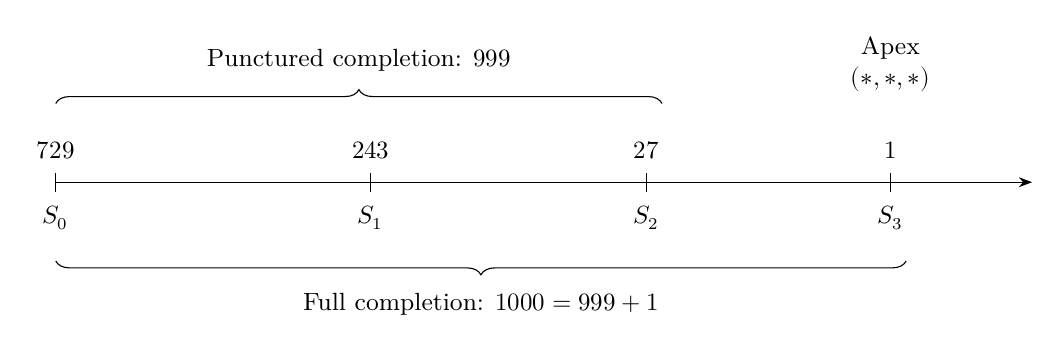
\begin{tikzpicture}[x=1cm,y=1cm,>=Stealth,font=\small]
\draw[->] (0,0)--(12.4,0);
\foreach \x/\a/\b in {0/729/{S_0},4.0/243/{S_1},7.5/27/{S_2},10.6/1/{S_3}}{
  \draw (\x,0.12)--(\x,-0.12);
  \node[above=5pt] at (\x,0) {\(\a\)};
  \node[below=5pt] at (\x,0) {\(\b\)};
}
\draw[decorate,decoration={brace,amplitude=5pt}] (0,1)--(7.7,1);
\node[above=8pt] at (3.85,1) {Punctured completion: \(999\)};
\draw[decorate,decoration={brace,mirror,amplitude=5pt}] (0,-1)--(10.8,-1);
\node[below=8pt] at (5.4,-1) {Full completion: \(1000=999+1\)};
\node[align=center] at (10.6,1.5) {Apex\\\((\ast,\ast,\ast)\)};
\end{tikzpicture}
\caption{Strata of the cubic completion. The layout represents
the set-theoretic decomposition, not a metric scale. The \(243\) elements
of \(S_1\) form three coordinate strata of \(81\) elements; the \(27\)
elements of \(S_2\) form three strata of \(9\). The apex completes the partition.}
\label{fig:revision-emrh}
\end{figure}

% BEGIN IX03_CUBIC_COMPLETION_FIGURE
% Original grayscale vector figure, included without redesign.
\begin{figure}[htbp]
\centering
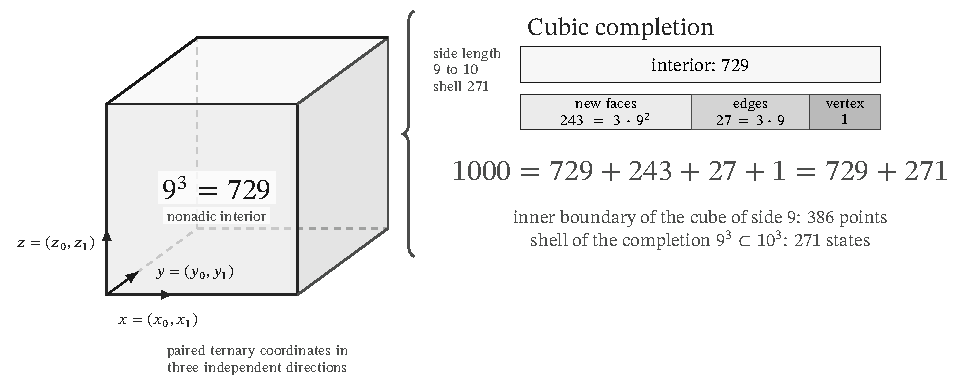
\includegraphics[width=\linewidth,keepaspectratio]{figures/cubo_emrh.pdf}
\caption{Cubic representation of the expansion from nine to ten classes per coordinate. Strata \(S_1,S_2,S_3\) locate the added incidences on faces, edges, and the apex; their cardinalities form the \(271\)-element shell. The \(386\)-element boundary belongs to the initial cube. This geometric perspective complements the partition in Figure~\ref{fig:revision-emrh}; graphical spacing is schematic.}
\label{fig:completacion-cubo-recuperado}
\end{figure}

% END IX03_CUBIC_COMPLETION_FIGURE

\subsubsection{Preservation of unity and dimensional compatibility}

Normalization is not limited to dividing an isolated identity. In dimension
\(d\), the product \(\widehat E^d\) carries the uniform measure
\(\mu_d(\{x\})=10^{-d}\). The coordinate projection
\(p_d:\widehat E^{d+1}\to\widehat E^d\) removes the last coordinate.

\begin{proposition}[Projective compatibility of the normalized measures]
For every \(d\geq1\),
\[
 (p_d)_*\mu_{d+1}=\mu_d,
 \qquad \mu_d(\widehat E^d)=1.
\]
The mass of the stratum with \(r\) additional coordinates is
\(\binom dr9^{d-r}/10^d\), and the sum of the masses of all strata
is one.
\end{proposition}
\begin{proof}
Each point of \(\widehat E^d\) has ten preimages. Their total mass is
\(10\,10^{-(d+1)}=10^{-d}\). Equality for any subset
follows by summing over its points. The stratified formula follows
from the same count as \eqref{eq:revision-estratos}; the binomial
\((9+1)^d\) gives the total normalization.
\end{proof}

In dimension three, removing the apex leaves mass \(999/1000\), and
restoring it adds \(1/1000\). Renormalizing before restoration
would define another measure: the distinction is operationally relevant.
In particular, preservation of probability mass, preservation of transport
registers, and thermodynamic dissipation are statements about
different objects. The proposition proves the first and provides the
compatible support for studying the second; the third requires a
specified dynamical and energetic realization.

The internal geometric boundary also remains distinct.
On the Cartesian representative \(\{1,\ldots,9\}^3\), removing
\(\{2,\ldots,8\}^3\) leaves \(386\) points. This boundary belongs to the
initial cube, whereas \(\widehat C\setminus C\) belongs to its
enlargement. The cubic completion, the positional base-thousand expansion, and
the exceptional incidence readout share support data;
their respective maps determine which information from those data
each representation uses.


% Fragmento conservado; véase MANIFIESTO_ANTECEDENTES_LECTURA.json.
% Incorporación al final de extension.tex; no contiene una sección principal.
% Procedencia: RESULTADO_RECUPERADO; explicitación sectorial de las hipótesis.
% Fuentes leídas: monografía Doble proyección holográfica (cantera editorial),
% manuscrito/local/01_tesis_recuperada.tex y
% manuscrito/generated/algebra_holonomica.tex, especialmente §§1--7 y 21.
% Definición rectora de número: manuscrito/flattened/main_autosuficiente.tex,
% secciones que comienzan en líneas 22137 y 23000 de la cantera de 775 páginas.
% No se adopta su presentación global como prueba de todas las flechas TPK.

\subsection{Number as a compatible section and value as a readout}
\label{hist:seccion}

The distinction between state and observation makes it possible to specify which object is
prolonged as resolution increases. At depth \(n\), let \(X_n\)
be the set of admissible states produced by APP--TRIT--TPK. Their data
include position, sum and product sheets, residues and quotients, regime,
orientation, carry, phase, route, boundary, memory, and survival. These are not
independent coordinates: preceding arithmetic evaluations and transports
impose their relations. A prolongation preserves those relations
in each antecedent, even as it adds new steps and new memory data.
This is the meaning of the arithmetic of histories developed in
\textup{(provenance preserved in the technical record)}.

Let \(r_{m,n}:X_m\to X_n\), for \(m\geq n\), be the depth
restrictions, with \(r_{n,n}=\operatorname{id}\) and
\(r_{\ell,n}=r_{m,n}\circ r_{\ell,m}\). Each restriction preserves the
prefix and the information already determined in it.

\begin{definition}[Compatible numerical section]
An HMT number is a compatible history of the state system:
\begin{equation}
 x=(x_n)_{n\geq0}\in X_\infty:=\varprojlim_n X_n,
 \qquad r_{m,n}(x_m)=x_n.
 \label{hist:limite-inverso}
\end{equation}
A readout is an additional operation on a specified domain of these
histories. A digit is a finite observation; a scalar value is an
evaluation of the readout. The pair consisting of the section and its readout constitutes
a read presentation, not a redefinition of the section's identity.
\end{definition}

On the Archimedean domain \(X_\infty^{\mathrm{Arch}}\), the readout associates
a closed cylinder with each prefix, preserves their nesting, and makes
their diameter tend to zero. It thus determines
\begin{equation}
 \operatorname{ev}_{\mathbb R}:X_\infty^{\mathrm{Arch}}\longrightarrow
 \mathbb R,\qquad
 \{\operatorname{ev}_{\mathbb R}(x)\}=\bigcap_n I_n(x).
 \label{hist:evaluacion}
\end{equation}
The concrete construction of these cylinders and the determination of their boundaries
are developed in Section~\ref{sec:generacion}. Definition
\eqref{hist:limite-inverso} does not by itself assert that the image of
\eqref{hist:evaluacion} is the entire line: a coverage assertion
requires its own theorem. Nor does equality of values establish, without
an injectivity result, equality of their histories. This separation
makes it possible to speak of precision as depth while preserving the difference
between the arithmetic antecedent and its scalar realization.

\subsection{Composition of histories and memory multiplier}
\label{hist:algebra}

Fix a sector of states at depth \(n\) and a category
\(\mathcal C\) whose arrows are their admissible histories. Composition
is written \(vu=v\circ u\): \(u\) is traversed first and then \(v\).
The elementary steps come from TPK selection, transport, and
updating. A local tritic fiber admits the expression
\(\mathbb R[J_x]/(J_x^2+\tau(x)1_x)\), where
\(\tau(x)\in\{+1,0,-1\}\). Regime and orientation belong to the
state being transported; a transition between regimes is not equivalent to
identifying their quadratic algebras.

The following formulation specifies an algebraic sector of this composition.
For each object \(x\), a unital associative real algebra \(A_x\) is given,
possibly noncommutative. For each \(u:x\to y\), a
unital homomorphism \(\rho_u:A_x\to A_y\) is given. We assume a strict action:
\begin{equation}
 \rho_{\operatorname{id}_x}=\operatorname{id}_{A_x},\qquad
 \rho_v\rho_u=\rho_{vu}.
 \label{hist:accion-estricta}
\end{equation}
For each composable pair \(u:x\to y\), \(v:y\to z\), fix an
invertible central multiplier
\(\Omega(v,u)\in Z(A_z)^\times\). We require the normalization
\(\Omega(\operatorname{id}_y,u)=\Omega(u,\operatorname{id}_x)=1_y\)
and, for each composable triple, the identity
\begin{equation}
 \rho_w\bigl(\Omega(v,u)\bigr)\Omega(w,vu)
   =\Omega(w,v)\Omega(wv,u).
 \label{hist:cociclo}
\end{equation}
These are explicit assumptions on the transports and their coefficients, not a
consequence of calling the dynamics holonomic. When this presentation is applied
to a TPK sector, its \(\rho_u\) and \(\Omega(v,u)\) must be identified.
Transitions expressed through bimodules require that structure to be
preserved and are not replaced by \eqref{hist:accion-estricta}.

The space of finite sums
\[
 \mathcal H(\mathcal C,A,\rho,\Omega)
   =\bigoplus_{u\in\operatorname{Mor}(\mathcal C)} A_{t(u)}T_u
\]
is equipped with the bilinear product
\begin{equation}
 (aT_v)(bT_u)=a\rho_v(b)\Omega(v,u)T_{vu},
 \label{hist:producto}
\end{equation}
if the arrows are composable, and zero otherwise. Here \(t(u)\)
denotes the terminal state. The sum brings together histories with coefficients; the
product concatenates histories while preserving the record multiplier.

\begin{proposition}[Sectorial associativity with a central multiplier]
Under \eqref{hist:accion-estricta} and \eqref{hist:cociclo}, the product
\eqref{hist:producto} is associative. If the set of objects is finite,
its unit is \(\sum_x1_xT_{\operatorname{id}_x}\).
\end{proposition}
\begin{proof}
For \(u:x\to y\), \(v:y\to z\), \(w:z\to t\), let
\(a\in A_y\), \(b\in A_z\), \(c\in A_t\). The two coefficients
of \(T_{wvu}\) are
\begin{align*}
 ((cT_w)(bT_v))(aT_u):\quad&
 c\rho_w(b)\Omega(w,v)\rho_{wv}(a)\Omega(wv,u),\\
 (cT_w)((bT_v)(aT_u)):\quad&
 c\rho_w(b)\rho_w\rho_v(a)\rho_w(\Omega(v,u))\Omega(w,vu).
\end{align*}
The strict action identifies \(\rho_w\rho_v(a)\) with \(\rho_{wv}(a)\).
Centrality of \(\Omega(w,v)\) allows it to be moved to the right of
that factor; \eqref{hist:cociclo} then equates the remaining products.
The coefficients \(a,b,c\) are not permuted. If the triple is not composable,
both parenthesizations are zero by their initial and terminal states.
Bilinearity completes the proof. The local identities and the
normalization of \(\Omega\) verify the indicated unit.
\end{proof}

The calendar carry provides an effective example. In the category
with one object and arrows \(C_9\), take coefficients
\(A=\mathbb R[z,z^{-1}]\), the identity action, and
\[
 \Omega(b,a)=z^{c_0(a,b)},\qquad
 c_0(a,b)=\left\lfloor\frac{a+b}{9}\right\rfloor,
 \quad 0\leq a,b<9.
\]
Both carry sums of a triple equal
\(\lfloor(a+b+c)/9\rfloor\); hence
\eqref{hist:cociclo} holds. The formal variable \(z\) records the winding without
assigning it a numerical value. Subsequently imposing \(z^{12}=1\) recovers the
dodecaphase record of the calendar \eqref{eq:extension108}; retaining
\(z\) without this relation distinguishes successive windings. The example realizes
the memory of this calendar, without identifying it with the entirety of
TPK memory.

\subsection{Double variance of refinement and conservation of unity}
\label{hist:doble-varianza}

Restricting states prolongs observables in the opposite direction.
Consider the function algebras, with pointwise product,
\(D_n=\operatorname{Fun}(X_n,\mathbb R)\). Precomposition defines
\begin{equation}
 r_{m,n}^*:D_n\longrightarrow D_m,
 \qquad r_{m,n}^*f=f\circ r_{m,n}.
 \label{hist:precomposicion}
\end{equation}
These are unital morphisms; they are also injective when the corresponding
restrictions are surjective. The direct limit
\(D_{\mathrm{cyl}}=\varinjlim_n(D_n,r_{n+1,n}^*)\) brings together
observations of finite depth. This algebra is not identified here
with the entire route algebra: prolonging the transport operators also requires
their compatibilities with refinement.

\begin{lemma}[Unity and naturality of evaluation]
If \(e_x\) is the indicator of \(x\in X_n\), then
\begin{equation}
 r_{m,n}^*e_x=\sum_{y:\,r_{m,n}(y)=x}e_y,
 \qquad r_{m,n}^*1_n=1_m,
 \label{hist:unidad}
\end{equation}
and, for every \(f\in D_n\), \(y\in X_m\),
\[
 \langle r_{m,n}^*f,y\rangle=\langle f,r_{m,n}y\rangle.
\]
Each section \(x\in X_\infty\) determines a well-defined evaluation
\(D_{\mathrm{cyl}}\to\mathbb R\), given by \([f]\mapsto f(x_n)\)
for \(f\in D_n\).
\end{lemma}
\begin{proof}
The fibers of \(r_{m,n}\) partition \(X_m\). Their
indicators are orthogonal and sum to \(1_m\), proving
\eqref{hist:unidad}. Naturality is the definition of precomposition.
Finally, \((r_{m,n}^*f)(x_m)=f(x_n)\), so that two compatible
representatives give the same evaluation in the direct limit.
\end{proof}

Global unity is the constant function one over all possibilities;
the individual section selects a compatible history. Preserving the
former does not mean immobilizing the latter. Refinement may increase
the number of extensions and the depth of each history while maintaining
unity and all evaluations of its antecedents.


\clearpage
% Preserved fragment; see MANIFIESTO_ANTECEDENTES_LECTURA.json.
\section{Coinductive generation of \texorpdfstring{\(\pi,\varphi,e\)}{pi, phi, e} to arbitrary depth}
\label{sec:generacion}

The six-block emission is a finite stage of the construction, not a complete decimal expansion. Its role is to produce regions with multiplicity, orientation, and transport rules. Prolongation must preserve these data and determine a compatible collection of prefixes of arbitrary length. The term \emph{generation} denotes this operation; \emph{genealogy} denotes the reconstruction of its dependencies. Both notions are involved, but they serve different purposes.

\subsection{Orbits, regions, and characters of closure, propagation, and self-scaling}

For a word \(w=(w_1,\ldots,w_6)\), define
\[
 r(w)=(w_3,w_1,w_2,w_5,w_6,w_4),\qquad
 s(w)=(w_4,w_5,w_6,w_1,w_2,w_3).
\]
We have \(r^3=s^2=I\) and \(srs=r^{-1}\); these permutations therefore realize the dihedral group \(D_3\). The action preserves the catalogue and the multiplicities and commutes with \(\Psi\). The quotient of the \(243\) visible words has \(43\) orbits: thirty-eight of cardinality six and five of cardinality three.

The closure class is recognized by a fibre predicate: its six orientations have five emissions per word, total multiplicity \(1008\), and distribution \(432+4\cdot144\). There is exactly one orbit with these properties in the catalogue. To specify the other two selections, write \(f(w)=\#\Psi^{-1}(w)\), \(m(w)=\sum_{U\in\Psi^{-1}(w)}\operatorname{mult}(U)\), and \(\nu(w)=(n_0,n_1,n_2)\). The additive diagonal class of an emission is \(d(U)=[i+j]_9\) in indices from zero to eight; its additive signature retains this class and the orientation \(ES\) or \(NO\). Let \(\mathcal D(\mathcal O)\) be the set of these classes for all emissions over an orbit.

Among the orbits of size six, the joint predicate
\[
 f(w)=1,\qquad m(w)=144\quad(w\in\mathcal O),\qquad
 \mathcal D(\mathcal O)=\{0,3,6\}
\]
leaves exactly six orbits. In this sector, the census \(\nu=(2,3,1)\), the same as for closure, uniquely selects propagation; the census \(\nu=(2,2,2)\) uniquely selects self-scaling. The diagonal support cannot be omitted: without it there are four balanced single-preimage orbits of multiplicity \(144\), not one. Finally, the existence of an emission with \(d=6\) and orientation \(ES\) selects one representative of each orbit and yields
\begin{equation}
 w^{\rm cl}=010211,\qquad w^{\rm pr}=201101,\qquad w^{\rm au}=121200.
 \label{eq:palabras-regionales}
\end{equation}
These symbols first designate regions of the catalogue. Scalar identification will be established through their readouts; they are not chosen because they coincide with digits of a known constant.

The closure word \(010211\) has the following five preimages:
\begin{center}\small
\begin{tabular}{@{}lll r@{}}\toprule
Six-block emission&Multiplicative signature&Role&Multiplicity\\\midrule
\(501,614,498,169,272,272\)&\(555555\)&transverse&432\\
\(810,923,870,169,272,272\)&\(339555\)&positive orientation&144\\
\(810,983,810,169,272,272\)&\(393555\)&positive orientation&144\\
\(870,923,810,169,272,272\)&\(933555\)&positive orientation&144\\
\(870,923,810,418,674,521\)&\(933717\)&oriented return&144\\\bottomrule
\end{tabular}
\end{center}
The multiplicity \(432\) and the constant signature \(555555\) characterize the transverse region. They do not identify the central position \((5,5)\) of APP. Confusing a six-window signature with a position in the support would erase the distinction between numerical region and electronic structure.

The microfibre also has a precise bipartite morphology. Each emission is a product of an additive cursor class and a multiplicative class. The three positive regions share the same additive class of eighteen conditions; together they contain three multiplicative classes of eight conditions each. The transverse region has a product \(18\times24\); the three positive regions taken together, another \(18\times24\); and the return, a product \(18\times8\). The decomposition by emissions has five parts, whereas the decomposition into connected components of the bipartite graph has three. Both preserve the same \(1008\) seeds without reducing form to a cardinality.

\subsection{Finite transport and the prolongation boundary}

The endomorphisms \(L_0,L_1\) of the ternary word space act before the Archimedean realization. Their determination begins with the transitions of the arithmetic state, not with the prescription of two matrices. If \(U_t\) is the composite step of selection, transport, and update, the observed block satisfies
\[
 b_j^\chi=\Pi_6(x_j^\chi),\qquad
 x_{j+1}^\chi=U_{9j+9}\cdots U_{9j+1}(x_j^\chi),
 \qquad \chi\in\{\mathrm{cl},\mathrm{pr},\mathrm{au}\}.
\]
Six transitions are formed for each regime: two consecutive transitions in each of the three regions. The pairs of source and target matrices obtained in the record are
\[
\begin{array}{c|c|c|c}
X_0&Y_0&X_1&Y_1\\\hline
010211&012222&010211&002111\\
012222&010211&002111&110221\\
201101&121221&102011&012222\\
121221&102011&012222&102011\\
121200&112202&121020&010210\\
112202&121020&010210&010200
\end{array}
\]
Each string of six digits represents a row in \(\FF_3^6\). Since \(\det X_0=1\) and \(\det X_1=-1\) in \(\FF_3\), the equations \(X_aL_a=Y_a\) uniquely determine \(L_a=X_a^{-1}Y_a\). In this row-vector chart, they yield
\[
 L_0=\begin{pmatrix}
 2&2&2&1&2&1\\2&1&2&2&1&1\\1&0&0&1&0&2\\
 0&0&1&1&1&0\\2&2&2&0&2&1\\2&1&2&1&0&0
 \end{pmatrix},\quad
 L_1=\begin{pmatrix}
 2&1&2&0&2&2\\1&2&1&1&2&0\\1&2&1&1&1&2\\
 0&1&0&0&2&1\\2&0&2&1&0&1\\0&2&2&2&1&1
 \end{pmatrix}\quad(\bmod3).
\]
The schedule \((L_0,L_0,L_1,L_1)\) produces four new blocks of six components. Their concatenations form
\[
 w_6\longrightarrow w_{12}\longrightarrow w_{18}
 \longrightarrow w_{24}\longrightarrow w_{30}.
\]
The subscripts of \(w\) indicate accumulated length. The boundary \(R_{36}\) preserves the terminal structure and opens the prolongation relation; it is not renamed as a final periodic block that could be repeated indefinitely.

The identity \(L=X^{-1}Y\) proves uniqueness once the transitions are fixed; it does not replace the production of those transitions by \(U_t\). The provenance of their record and the examination of the sixteen binary schedules are documented in the technical supplement. The indicated schedule is the only one of these sixteen that jointly reproduces the three sequences of five blocks.

\subsection{Five closure regions and angular compensation}

The closure region contains one transverse component and four accompanying components. The symmetric readout acts on the space of its five positions through
\[
 P_5=\frac15\mathbf1\mathbf1^{\mathsf T},\qquad
 \mathbf1=(1,1,1,1,1)^{\mathsf T}.
\]
Invariance \(P_5\lambda=\lambda\) and conservation \(\mathbf1^{\mathsf T}\lambda=1\) force \(\lambda=\mathbf1/5\). This normalization distributes the unit among positions of the readout; it does not replace the seed multiplicities \(432,144,144,144,144\) with uniform frequencies. The elliptic chart of the readout realizes each coordinate through \(1+\lambda_jJ\); its slope is \(\lambda_j\), so the primitive slope is \(1/5\). This makes explicit the rule taking a normalized coordinate to a slope, rather than identifying the two notions without a map. The readout composes the four accompanying positions by the law
\begin{equation}
 a\oplus b=\frac{a+b}{1-ab}.
 \label{eq:suma-pendientes}
\end{equation}
This law is obtained by multiplying \((1+aJ)(1+bJ)\) in the regime \(J^2=-I\) and dividing by its scalar component. The composition of slopes is therefore a realization of the quadratic structure of TRIT, not an ordinary sum of four fractions.

\begin{proposition}[Closure compensator]
The composition of four slopes \(1/5\) is \(120/119\). The condition of return to slope one determines a unique positive compensator of the form \(1/q\), with \(q>1\), and yields \(q=239\).
\end{proposition}
\begin{proof}
The first doubling gives \((1/5)\oplus(1/5)=5/12\); the second, \((5/12)\oplus(5/12)=120/119\). The condition
\[
 \frac{120/119-1/q}{1+(120/119)/q}=1
\]
is equivalent to \((120-119)q=120+119\), hence \(q=239\).
\end{proof}

The resulting closure character has the realization
\begin{equation}
 \Pi_{\rm cl}=4\left(4\arctan\frac15-\arctan\frac1{239}\right).
 \label{eq:lector-pi}
\end{equation}
Machin's angular identity recognizes \(\Pi_{\rm cl}=\pi\). The direction of the construction is precise: the slope and the number of compositions are specified by the pentafibre readout; the compensation equation forces \(239\). Once this character has been produced, its evaluation by alternating series does not select the seed orbit anew.

For \(0<x<1\), the alternating sums
\[
 A_n(x)=\sum_{j=0}^n\frac{(-1)^jx^{2j+1}}{2j+1}
\]
enclose \(\arctan x\) between two consecutive truncations, with difference \(x^{2n+3}/(2n+3)\). Applied to the two slopes in \eqref{eq:lector-pi}, they provide rational endpoints with explicit error bounds. The numerical value is thus calculated as a consequence of the exact character, without introducing a target prefix.

\subsection{Propagation readout and normalization of the unit}

The propagation region is realized by a formal collection \(P_t\in\mathcal A[[t]]\), where \(\mathcal A\) is a unital commutative algebra over \(\QQ\). Its composition satisfies \(P_{t+s}=P_tP_s\), with unit \(P_0=1\), and the oriented elementary transport fixes the scalar generator \(P'_0=+1\). The condition fixes its sign, not merely its magnitude. Writing
\[
 P_t=\sum_{n\ge0}a_nt^n,
\]
the normalization determines \(a_0=a_1=1\). Comparing the coefficient of \(s^nt\) in \(P_{s+t}=P_sP_t\) gives \((n+1)a_{n+1}=a_na_1\); equivalently, \(P'_t=P_t\). Thus,
\begin{equation}
 (n+1)a_{n+1}=a_n,\qquad a_n=\frac1{n!}.
 \label{eq:propagacion}
\end{equation}
The character at one unit of the parameter is \(\Pi_{\rm pr}=P_1\), subsequently recognized as \(e\).

Normalization of the generator matters. Without this datum, the semigroup law would admit \(P_t=e^{ct}\) for different \(c\); the condition fixing the unit of the parameter in the readout is therefore not omitted. This condition precedes decimal comparison and belongs to the exposition of the operational rule, not to the choice of an experimental value.

\begin{proposition}[Rational propagation bounds]
For \(n\ge1\), let \(E_n=\sum_{j=0}^n1/j!\). Then
\[
 E_n<\Pi_{\rm pr}<E_n+\frac{n+2}{(n+1)(n+1)!}.
\]
\end{proposition}
\begin{proof}
The first omitted term is \(1/(n+1)!\). Each subsequent ratio is at most \(1/(n+2)\). The geometric upper bound for the tail is
\[
 \frac1{(n+1)!}\frac1{1-1/(n+2)}
 =\frac{n+2}{(n+1)(n+1)!}.
\]
Strict inequality follows from the decrease of the successive ratios.
\end{proof}

\subsection{Modal incidence and generation of self-scaling}

The tritic selector produces the cycle \((+1,-1,0)\). On the modes \(\Sigma,\Pi\), the rule is \(+1:m\mapsto\Sigma\), \(-1:m\mapsto\Pi\), \(0:m\mapsto m\). With cyclic closure, the observed mode is \((\Sigma,\Pi,\Pi)\). Its edges are \(\Sigma\to\Pi\), \(\Pi\to\Pi\), and \(\Pi\to\Sigma\). Its incidence, in this ordering of the modes, is therefore
\begin{equation}
 F_{\rm av}=\begin{pmatrix}0&1\\1&1\end{pmatrix}.
 \label{eq:fav}
\end{equation}
The four entries are obtained from the schedule, not from an equation that has already received the value of \(\varphi\). Repeating the schedule gives counts \(3F_{\rm av},9F_{\rm av},36F_{\rm av}\) at lengths nine, twenty-seven, and one hundred and eight. These counts are not powers of the matrix.

\begin{theorem}[Positive self-scaling character]
The incidence \eqref{eq:fav} has a unique strictly positive eigenray. When normalized as \((1,x)^{\mathsf T}\), its coordinate \(x\) satisfies \(x^2-x-1=0\), \(x>0\), and equals \(\varphi=(1+\sqrt5)/2\).
\end{theorem}
\begin{proof}
The eigenvalue equation gives \(x=\lambda\) and \(1+x=\lambda x\). Eliminating \(\lambda\) yields the polynomial. Only one of its two roots is positive. Since all entries of \(F_{\rm av}^2\) are positive, the positive ray is unique and simple. The radical expression recognizes the coordinate obtained; it does not participate in the production of \(F_{\rm av}\).
\end{proof}

With \(F_0=0,F_1=1,F_{n+1}=F_n+F_{n-1}\), the incidence induces, for \(n\geq1\),
\[
 F_{\rm av}^n=\begin{pmatrix}F_{n-1}&F_n\\F_n&F_{n+1}\end{pmatrix}.
\]
The consecutive ratios \(F_{n+1}/F_n\) alternate around \(\varphi\). The determinant identity
\[
 F_{n+1}^2-F_nF_{n+2}=(-1)^n
\]
gives an exact width \(1/(F_nF_{n+1})\) between two consecutive ratios. Their growth makes this rational bracket arbitrarily narrow.

\subsection{Compatible cylinders and arbitrary depth}

The realization of a ternary block \(b=(b_1,\ldots,b_6)\) is the integer
\[
 \nu(b)=\sum_{j=1}^6b_j3^{6-j}\in\{0,\ldots,728\}.
\]
A sequence of blocks defines integer prefixes by \(N_{n+1}=729N_n+\nu(b_{n+1})\), starting from \(N_0=m\), where \(m\) is the integer part determined by the readout. The preceding brackets place the closure, propagation, and self-scaling characters in \((3,4)\), \((2,3)\), and \((1,2)\), respectively; their initial values are therefore \(m=3,2,1\). Subsequent blocks refine the fractional part. The corresponding cylinder is
\begin{equation}
 I_n=\left[\frac{N_n}{729^n},\frac{N_n+1}{729^n}\right],
 \qquad |I_n|=729^{-n}.
 \label{eq:cilindro}
\end{equation}
The half-open convention is used to select a representative when a value lies on a boundary. Passage to the limit uses the closures of these intervals and identifies the two equivalent boundary expansions. This qualification prevents the assumption that every intersection of nested half-open intervals is automatically nonempty.

\begin{theorem}[Determination of the scalar realization]
A compatible block history determines a unique limit of the left endpoints of \eqref{eq:cilindro}. If an exact character has rational brackets of arbitrarily small width and is separated from the boundary of every decimal cylinder examined, each decimal prefix of finite length is determined after a finite computation. The prefixes thus obtained are mutually compatible.
\end{theorem}
\begin{proof}
Extending a block preserves the previous prefix by Euclidean division. The closed cylinders are nested and their diameter tends to zero; their left endpoints form a Cauchy sequence and have a unique limit. For a fixed decimal length, a value separated from the boundaries of the partition has positive distance from them. A sufficiently narrow bracket lies within a single cell and determines its prefix. Uniqueness of the cell and nesting of the partitions prove compatibility under truncation. At points with a terminating expansion, the exact boundary decision and its representation convention must be added; this decision does not follow from numerical width alone.
\end{proof}

\begin{corollary}[Finite determination and compatibility of regional prefixes]
\label{gen:prefijos-regionales}
For each of the realizations \(\pi,\varphi,e\) and every finite
decimal length, the constructed brackets determine the corresponding prefix
by a finite computation. The prefixes obtained at different depths
are compatible under truncation.
\end{corollary}
\begin{proof}
The closure, propagation, and self-scaling characters have the
preceding brackets. After their recognition, the irrationality of \(\pi,e,\varphi\)
ensures their separation from the rational boundaries of every finite decimal
partition. The preceding theorem applies to each character.
\end{proof}
Arbitrary depth expresses the quantifier in the corollary: for every
finite horizon there is a computation determining its prefix. The mathematical
object is the complete compatible collection; each execution obtains a
finite projection of it.

\subsection{Specular involution and synchronization of the regions}

The joint nonadic connection transports the three characters together. In the ninth-phase chart, the self-scaling axis and the ternary sum of closure and propagation remain fixed under specular interchange. Helical inversion changes the direction of transport; the mirror of the two channels changes their relative orientation. These are different involutions, although both act on the same trajectory system.

The matching census values illustrate this coordination:
\begin{center}
\begin{tabular}{@{}c rrr l@{}}\toprule
Phase&\(N_\pi\)&\(N_e\)&\(N_\varphi\)&Equality of counts\\\midrule
4&207&207&122&\(N_\pi=N_e\)\\
5&39&151&151&\(N_e=N_\varphi\)\\
6&110&110&69&\(N_\pi=N_e\)\\
7&81&29&81&\(N_\varphi=N_\pi\)\\
8&59&59&59&triple synchronization\\
9&43&43&43&triple synchronization\\\bottomrule
\end{tabular}
\end{center}
These integers count compatible coordinates of the regions. They do not assert equality between \(\pi\), \(e\), and \(\varphi\) as real numbers. If
\[
 \partial(a,b,c)=(a-b,b-c,c-a),
\]
its image belongs to the lattice \(A_2=\{(u,v,w)\in\ZZ^3:u+v+w=0\}\). In phases eight and nine the relative component vanishes, but the diagonal component changes from \((59,59,59)\) to \((43,43,43)\). Relative synchronization coexists with a shift of \(-16\) per channel. The closure that will lead to \(\alpha\) must preserve both pieces of information: relative coincidence and memory evolution.


% Fragmento conservado; véase MANIFIESTO_ANTECEDENTES_LECTURA.json.
\subsection{Mirror symmetry of the regions and double realization}
\label{mono-ampl:regiones}

The mirror exchange acts on the regional block
\(B=(u^\pi,u^e,u^\varphi)\in(\mathbb F_3^6)^3\) by
\[
 \mathfrak cB=(u^e,u^\pi,u^\varphi).
\]
Its fixed axis and aggregate are, respectively, \(u^\varphi\) and
\(s=u^\pi+u^e\). This fixedness concerns the involution on a fiber;
both coordinates may evolve during nonadic transport.
With \(q=u^\pi+u^e+u^\varphi\),
\(a=u^\pi+u^e-u^\varphi\), and \(d=u^\pi-u^e\), one recovers
\[
 u^\varphi=2(q-a),\qquad s=q-u^\varphi,\qquad
 u^\pi=2(s+d),\qquad u^e=2(s-d).
\]
The equalities hold componentwise in \(\mathbb F_3\), where
\(2^{-1}=2\). The mirror preserves \(q,a,s\) and reverses \(d\); this
antisymmetric coordinate individualizes the distribution preserved
by the aggregate without distinction. The inversion \(\mathcal I\) of the time index and the
channel involution \(\mathfrak c\) consequently act on
different data.

Phase return has an explicit witness:
\[
 \begin{aligned}
 B_1&=(012222\mid121221\mid112202),\\
 B_{10}&=(101222\mid112221\mid112002).
 \end{aligned}
\]
Both positions have phase \(1\); the block, axis, and memory have
changed. Likewise, synchronization of the censuses at phases \(8\) and
\(9\) cancels their relative differences, while the diagonal component
changes from \((59,59,59)\) to \((43,43,43)\). Equality of a relative observable
does not exhaust the state determining it.

The double realization preserves this architecture. In Section
8.1 of Article I (provenance of the exceptional corridor, preserved in the technical record), the same prefix determines nested
cylinders on the one hand and a sequence of encoded words with their frames on the other.
The first map passes to the limit through contraction of diameters; the second
satisfies \(r_{n,m}Q_n=Q_mp_{n,m}\) and defines \(Q_\infty\).
Figure \ref{mono-ampl:fig-regional} anticipates these two maps.
The subsequent incidence progression constructs codes, lattices, and the
Moonshine realization on their own domains; the automorphism group
acts on that realization, not on the digits through an
implicit identification.

% Fragmento conservado; véase MANIFIESTO_ANTECEDENTES_LECTURA.json.
% Figura acumulativa; destino figures/monodromia_regional_ampliacion.tex.
\begin{figure}[!htbp]
\centering
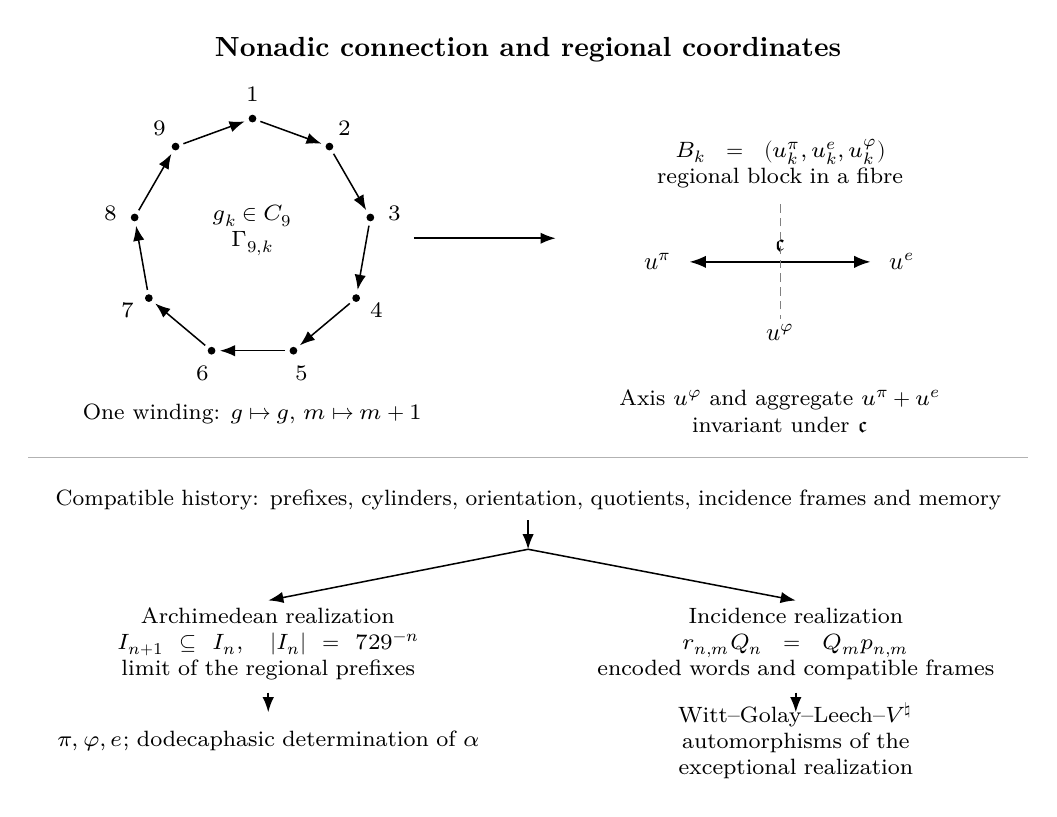
\begin{tikzpicture}[x=1cm,y=1cm,>=Latex,font=\small,
  flow/.style={->,line width=.55pt},
  ann/.style={align=center,font=\footnotesize}]
\node[font=\bfseries] at (6.9,9.2)
  {Nonadic connection and regional coordinates};
\begin{scope}[shift={(3.4,6.8)}]
 \foreach \k in {1,...,9}{
  \pgfmathsetmacro{\ang}{90-40*(\k-1)}
  \coordinate (p\k) at (\ang:1.52);
  \fill (p\k) circle (1.4pt);
  \node[fill=white,inner sep=1.1pt,font=\footnotesize]
    at (\ang:1.83) {\(\k\)};
 }
 \foreach \k in {1,...,8}{
  \pgfmathtruncatemacro{\next}{\k+1}
  \draw[flow,shorten >=3pt,shorten <=3pt] (p\k)--(p\next);
 }
 \draw[flow,shorten >=3pt,shorten <=3pt] (p9)--(p1);
 \node[ann] at (0,.1) {\(g_k\in C_9\)\\\(\Gamma_{9,k}\)};
 \node[ann] at (0,-2.23) {One winding: \(g\mapsto g\), \(m\mapsto m+1\)};
\end{scope}
\node[ann,text width=5.25cm] at (10.1,7.75)
 {\(B_k=(u_k^\pi,u_k^e,u_k^\varphi)\)\\
 regional block in a fibre};
\node at (8.55,6.5) {\(u^\pi\)};
\node at (11.65,6.5) {\(u^e\)};
\draw[<->,line width=.65pt] (8.95,6.5)--node[above]{\(\mathfrak c\)}(11.25,6.5);
\draw[densely dashed,gray] (10.1,5.72)--(10.1,7.23);
\node[fill=white,inner sep=2pt] at (10.1,5.6){\(u^\varphi\)};
\node[ann] at (10.1,4.6)
 {Axis \(u^\varphi\) and aggregate \(u^\pi+u^e\)\\
 invariant under \(\mathfrak c\)};
\draw[flow] (5.45,6.8)--(7.25,6.8);
\draw[gray!60,line width=.3pt] (.55,4.02)--(13.25,4.02);
\node[ann,text width=12cm] (hist) at (6.9,3.47)
 {Compatible history: prefixes, cylinders, orientation, quotients,
 incidence frames and memory};
\coordinate (fork) at (6.9,2.85);
\draw[flow] (hist.south)--(fork);
\draw[flow] (fork)--(3.6,2.2);
\draw[flow] (fork)--(10.3,2.2);
\node[ann,text width=5.6cm] at (3.6,1.65)
 {Archimedean realization\\
 \(I_{n+1}\subseteq I_n,\quad |I_n|=729^{-n}\)\\
 limit of the regional prefixes};
\node[ann,text width=5.6cm] at (10.3,1.65)
 {Incidence realization\\
 \(r_{n,m}Q_n=Q_mp_{n,m}\)\\
 encoded words and compatible frames};
\node[ann,text width=5.6cm] at (3.6,.42)
 {\(\pi,\varphi,e\); dodecaphasic determination of \(\alpha\)};
\node[ann,text width=5.6cm] at (10.3,.42)
 {Witt--Golay--Leech--\(V^\natural\)\\
 automorphisms of the exceptional realization};
\draw[flow] (3.6,1.03)--(3.6,.78);
\draw[flow] (10.3,1.03)--(10.3,.78);
\end{tikzpicture}
\caption{\fontsize{9}{11}\selectfont Nine phases of a connection and two realizations of the compatible
history. The cycle represents phase; each winding increments the counter.
The regional diagram represents the involution \(\mathfrak c\), which
interchanges closure and propagation and fixes the self-scale axis in a fibre.
This invariance does not require the axis to remain constant during transport.
The two lower maps use the same prefix: one determines
its numerical limit and the other preserves words and incidence frames. The
maps of this second realization are specified in Section
8.1 of Article I (provenance of the exceptional corridor, preserved in the technical register); the exceptional route is developed afterwards.}
\label{mono-ampl:fig-regional}
\end{figure}


\clearpage
% BEGIN NUCLEO_ADITIVO_20260921_SELECCION
\clearpage
% Demonstrative expansion DF003--DF007. The integral source is unchanged.
% Common owner of the Lean files cited in these comments:
% output/PAQUETE_ARTICULO_I_INTEGRACION_ESTADO_CAMPOS_20260919/.
% Causal placement of the first section: after the coinductive regional
% readers and before their registers are used as inputs to K selection.
% Causal placement of the second section: after the marked
% Paley--Witt--Golay--Leech construction and before reconstruction of the VOA.
% Both expository cuts preserve the same APP--TRIT--TPK origin.

\section[Regional generation and refinement]{Integral compatibility of regional generation, cylindrical refinement, and incidence}
\label{act21:sec:df-lectores-cilindros}

Regional prolongation produces ordered sequences of blocks together with
their reading depths. The Archimedean projection and ternary incidence
are calculated on these same sequences. The connection between the two
realizations can be formulated entirely through integer operations:
selection by rational intervals, Euclidean division, lifting of six
trits, carry reading, and the Witt transformation. This formulation makes
it possible to trace each coefficient from its generating block to its
subsequent use.

The construction uses the three regional readers already obtained from the
APP--TRIT--TPK state. We denote them by the indices
\(c\in\{\mathrm P,\mathrm E,\mathrm F\}\), corresponding, respectively,
to the closure, propagation, and autoscaling regions. Their real realization
will be written as \(v_c\). The subsequent identifications
\(v_{\mathrm P}=\pi_{\mathrm{HMT}}\),
\(v_{\mathrm E}=e_{\mathrm{HMT}}\), and
\(v_{\mathrm F}=\varphi_{\mathrm{HMT}}\) preserve this causal order.
The operation that emits a block inspects the rational intervals of the
regional reader; the real value enters the proof of correctness of that
operation.

\subsection{Positional emission through rational separation of cells}
\label{act21:subsec:df-emision-racional}

% Source: lean/biblioteca/RegionalPublicationComposition.lean,
% produced_brackets, eventual_publication, joint_eventual_publication,
% search_terminates, stopped_cell_correct, publications_compatible.

For each region, two rational sequences
\(\ell_c(j),u_c(j)\), constructed by its reader, are available and satisfy
\[
 \ell_c(j)\leq v_c\leq u_c(j).
\]
The cell-separation property proved for these readers states that, for
each integer \(s>0\), there exists \(J\) such that, for every \(j\geq J\),
\begin{equation}
 \lfloor s\ell_c(j)\rfloor
 =\lceil su_c(j)\rceil-1
 =\lfloor sv_c\rfloor.
 \label{act21:eq:df-separacion-celdas}
\end{equation}
Avoidance of rational boundaries by the regional values is the hypothesis
of the preceding theorems that guarantees this separation. Here we use
their operational conclusion together with the readers and intervals
that produce it.

\begin{definition}[Separation index and emitted prefix]
For \(s>0\), let
\[
 j_c(s)=\min\{j\in\mathbb N:
 \lfloor s\ell_c(j)\rfloor=\lceil su_c(j)\rceil-1\}.
\]
For an integer base \(b\geq2\) and a depth \(n\geq0\), define
\begin{equation}
 P_c(b,n)=\lfloor b^n\ell_c(j_c(b^n))\rfloor.
 \label{act21:eq:df-publicacion-prefijo}
\end{equation}
The prefix contains the integer part and the first \(n\) positions in base
\(b\); consequently, \(P_c(b,0)\) is the regional integer part.
\end{definition}

\begin{theorem}[Termination and correctness of emission]
\label{act21:thm:df-emision-correcta}
The index \(j_c(s)\) exists for every \(s>0\). The emitted prefixes satisfy
\begin{equation}
 P_c(b,n)=\lfloor b^n v_c\rfloor,
 \qquad
 P_c(b,n)\leq b^n v_c<P_c(b,n)+1.
 \label{act21:eq:df-prefijo-correcto}
\end{equation}
For each scale \(s\), a single sufficiency index \(J(s)\) can also be
chosen that is valid simultaneously for all three regions.
\end{theorem}

\begin{proof}
The eventual equality in \eqref{act21:eq:df-separacion-celdas} makes the set
defining \(j_c(s)\) nonempty. Its minimum exists by the well-ordering of
\(\mathbb N\). At any index where the equality holds, the rational lower
bound gives
\(\lfloor s\ell_c(j)\rfloor\leq\lfloor sv_c\rfloor\).
The upper bound, together with avoidance of a cell boundary, gives
\(\lfloor sv_c\rfloor\leq\lceil su_c(j)\rceil-1\).
When the two integer endpoints coincide, the intervening integer coincides
with them. This proves \eqref{act21:eq:df-prefijo-correcto}. For the joint
statement, it suffices to take the maximum of the three sufficiency indices
obtained at the same scale. The joint index controls all three emissions
simultaneously, while each region retains its own intervals.
\end{proof}

\begin{proposition}[Exact compatibility of prefixes]
\label{act21:prop:df-prefijos-compatibles}
For \(n,m\geq0\),
\begin{equation}
 \left\lfloor\frac{P_c(b,n+m)}{b^m}\right\rfloor=P_c(b,n).
 \label{act21:eq:df-truncamiento}
\end{equation}
In particular, the next block
\(d_c(b,n)=P_c(b,n+1)\bmod b\) satisfies
\begin{equation}
 P_c(b,n+1)=bP_c(b,n)+d_c(b,n),\qquad 0\leq d_c(b,n)<b.
 \label{act21:eq:df-paso-posicional}
\end{equation}
\end{proposition}

\begin{proof}
Write \(b^n v_c=N+\theta\), with
\(N=P_c(b,n)\) and \(0\leq\theta<1\). Then
\(P_c(b,n+m)=b^mN+\lfloor b^m\theta\rfloor\), and the second summand
belongs to \(\{0,\ldots,b^m-1\}\). Euclidean division by \(b^m\)
recovers \(N\). The specialization \(m=1\) yields
\eqref{act21:eq:df-paso-posicional} and its residual bound.
\end{proof}

\subsection{Regional blocks of six trits at arbitrary depth}
\label{act21:subsec:df-bloques-arbitrarios}

% Source: deltas/integracion/JointRegionalFrontier.lean,
% publish_base729_eq_base3, generated_block_from_longer_prefix,
% generated_block_eq_finite, generated_signature_eq_finite.

The integer equality \(729=3^6\) determines the grouping of six ternary
positions into a block. For \(t\geq0\), define
\begin{equation}
 u_c(t)=P_c(729,t+1)\bmod729,
 \qquad
 B_{c,j}(t)=
 \left\lfloor\frac{u_c(t)}{3^{5-j}}\right\rfloor\bmod3,
 \quad 0\leq j<6.
 \label{act21:eq:df-bloque-y-banda}
\end{equation}
Thus \(B_c(t)\) is an ordered word of six trits, and
\begin{equation}
 u_c(t)=\sum_{j=0}^{5}B_{c,j}(t)3^{5-j}.
 \label{act21:eq:df-elevacion-banda}
\end{equation}
The word and its integer lift are mutually recoverable representations
of the same emitted block.

\begin{theorem}[Stability of extraction at any depth]
\label{act21:thm:df-bloque-estable}
For every \(n\),
\[
 P_c(729,n)=P_c(3,6n).
\]
If \(t<n\), then
\begin{equation}
 u_c(t)=
 \left\lfloor\frac{P_c(729,n)}{729^{n-t-1}}\right\rfloor\bmod729.
 \label{act21:eq:df-bloque-prefijo-largo}
\end{equation}
Consequently, every extension of the prefix preserves all previously
emitted blocks and all signatures calculated from them.
\end{theorem}

\begin{proof}
The first equality follows because both prefixes are separated at the same
scale, \(729^n=3^{6n}\), and from
Theorem~\ref{act21:thm:df-emision-correcta}. For the second, apply
\eqref{act21:eq:df-truncamiento} at depths \(n\) and \(t+1\), and then take
the residue modulo \(729\). The ternary extraction in
\eqref{act21:eq:df-bloque-y-banda} is deterministic. Any explicit function of
those eighteen coordinates therefore retains the same result when the
prefix is extended.
\end{proof}

The construction is quantified over \(t\in\mathbb N\). A table
materializing one hundred blocks is a finite evaluation of this
construction; formula \eqref{act21:eq:df-bloque-prefijo-largo} determines its
compatibility with every subsequent extension exactly.

\begin{example}[First joint block]
Evaluation of the selected regional readers gives the words
\[
 B_{\mathrm P}(0)=010211,\qquad
 B_{\mathrm E}(0)=201101,\qquad
 B_{\mathrm F}(0)=121200.
\]
Their lifting by \eqref{act21:eq:df-elevacion-banda} produces
\[
 u_{\mathrm P}(0)=103,\qquad
 u_{\mathrm E}(0)=523,\qquad
 u_{\mathrm F}(0)=450.
\]
For example,
\(201101_3=2\cdot243+27+9+1=523\).
All six positions, including leading zeros, are retained in the band
representation. The leading zero in \(010211\) has a defined position
even though the decimal notation for \(103\) does not contain it.
\end{example}

\subsection{Transition registers and reconstruction of linear lifts}
\label{act21:subsec:df-registros-transicion}

% Sources: deltas/integracion/RegionalTransitionRecords.lean and
% GeneratedTransitionRecords.lean; lean/biblioteca/TPKLifts.lean.
% The reconstructed links are R(0)->R(1) and R(2)->R(3).

Over \(\mathbb F_3\), collect two consecutive emissions from each region
in the matrix
\begin{equation}
 R(t)=
 \begin{pmatrix}
 B_{\mathrm P}(t)\\ B_{\mathrm P}(t+1)\\
 B_{\mathrm E}(t)\\ B_{\mathrm E}(t+1)\\
 B_{\mathrm F}(t)\\ B_{\mathrm F}(t+1)
 \end{pmatrix}.
 \label{act21:eq:df-registro-matricial}
\end{equation}
This definition fixes both the regional order and the temporal order.
The first four registers are
\[
 X_0=R(0),\quad Y_0=R(1),\quad X_1=R(2),\quad Y_1=R(3).
\]
Their values, obtained by extraction from the regional prefixes, are
\begin{align*}
 X_0&=\begin{pmatrix}
0&1&0&2&1&1\\0&1&2&2&2&2\\2&0&1&1&0&1\\
1&2&1&2&2&1\\1&2&1&2&0&0\\1&1&2&2&0&2
\end{pmatrix},&
 Y_0&=\begin{pmatrix}
0&1&2&2&2&2\\0&1&0&2&1&1\\1&2&1&2&2&1\\
1&0&2&0&1&1\\1&1&2&2&0&2\\1&2&1&0&2&0
\end{pmatrix},\\[1ex]
 X_1&=\begin{pmatrix}
0&1&0&2&1&1\\0&0&2&1&1&1\\1&0&2&0&1&1\\
0&1&2&2&2&2\\1&2&1&0&2&0\\0&1&0&2&1&0
\end{pmatrix},&
 Y_1&=\begin{pmatrix}
0&0&2&1&1&1\\1&1&0&2&2&1\\0&1&2&2&2&2\\
1&0&2&0&1&1\\0&1&0&2&1&0\\0&1&0&2&0&0
\end{pmatrix}.
\end{align*}

\begin{theorem}[Unique reconstruction of the two initial links]
\label{act21:thm:df-elevaciones-reconstruidas}
The equations \(X_0L_0=Y_0\) and \(X_1L_1=Y_1\) each have a unique
solution in \(M_6(\mathbb F_3)\). These solutions are
\begin{align*}
 L_0&=\begin{pmatrix}
2&2&2&1&2&1\\2&1&2&2&1&1\\1&0&0&1&0&2\\
0&0&1&1&1&0\\2&2&2&0&2&1\\2&1&2&1&0&0
\end{pmatrix},&
 L_1&=\begin{pmatrix}
2&1&2&0&2&2\\1&2&1&1&2&0\\1&2&1&1&1&2\\
0&1&0&0&2&1\\2&0&2&1&0&1\\0&2&2&2&1&1
\end{pmatrix}.
\end{align*}
Both matrices are invertible.
\end{theorem}

\begin{proof}
The matrices
\begin{align*}
 A_0&=\begin{pmatrix}
1&1&2&0&1&2\\0&0&1&0&0&1\\2&1&2&1&0&1\\
0&2&0&1&0&2\\2&1&1&0&2&2\\2&1&1&1&1&2
\end{pmatrix},&
 A_1&=\begin{pmatrix}
1&0&1&2&0&0\\0&0&1&1&2&2\\0&1&2&0&1&1\\
1&1&0&2&0&0\\1&1&2&1&1&2\\1&0&0&0&0&2
\end{pmatrix}
\end{align*}
satisfy \(A_iX_i=X_iA_i=I\), by multiplication in \(\mathbb F_3\).
The solutions are therefore forced by \(L_i=A_iY_i\); multiplication
produces the two displayed matrices. Their inverses are
\begin{align*}
 L_0^{-1}&=\begin{pmatrix}
1&2&0&2&0&2\\2&0&2&2&0&0\\2&1&2&0&2&0\\
1&0&0&0&2&0\\0&2&1&1&2&0\\2&2&2&2&2&2
\end{pmatrix},&
 L_1^{-1}&=\begin{pmatrix}
2&0&2&1&2&1\\2&1&0&0&2&0\\2&0&2&2&0&2\\
2&0&0&1&1&0\\1&1&1&1&1&0\\2&0&1&2&2&0
\end{pmatrix}.
\end{align*}
The bilateral verification \(L_iL_i^{-1}=L_i^{-1}L_i=I\) proves exact
recovery of each transformed word. All products use residues \(0,1,2\)
with their interpretation in \(\mathbb F_3\).
\end{proof}

The causal reading of this result is precise: the regional emissions
produce \(R(t)\); the registers \(R(0),\ldots,R(3)\) determine the two
lifts above; their inverses recover the transformed words. Continuity
for every \(t\) belongs to the coinductive readers and
Theorem~\ref{act21:thm:df-bloque-estable}. The matrix reconstruction proved here
has the two links specified in its statement as its domain.

\subsection{Simultaneous refinement in ternary and decimal bases}
\label{act21:subsec:df-cilindros-mixtos}

% Source: deltas/integracion/RegionalCylinderTransition.lean.

A ternary emission of six trits and a decimal emission of three digits
are readings in different bases. To preserve their relationship, record
the state
\[
 s=(n,k,N,D),
\]
where \(N\) is a prefix at depth \(n\) in base \(729\), and \(D\) is
a prefix at depth \(k\) in base \(1000\). Their Archimedean cylinders are
\begin{equation}
 I_{729}(s)=\left[\frac{N}{729^n},\frac{N+1}{729^n}\right),\qquad
 I_{1000}(s)=\left[\frac{D}{1000^k},\frac{D+1}{1000^k}\right).
 \label{act21:eq:df-cilindros}
\end{equation}
The half-open upper endpoint assigns each value to a unique cell at a
given base and depth.

\begin{definition}[Integer compatibility defects]
Define
\begin{align}
 A(s)&=N1000^k-D729^n,\label{act21:eq:df-defecto-inferior}\\
 B(s)&=(N+1)1000^k-D729^n=A(s)+1000^k.
 \label{act21:eq:df-defecto-superior}
\end{align}
The state is compatible when
\begin{equation}
 A(s)<729^n,\qquad B(s)>0.
 \label{act21:eq:df-compatibilidad}
\end{equation}
\end{definition}

\begin{lemma}[Integer criterion for intersection]
The cylinders in \eqref{act21:eq:df-cilindros} have a nonempty intersection if
and only if \eqref{act21:eq:df-compatibilidad} holds.
\end{lemma}

\begin{proof}
Two half-open intervals \([a,b)\) and \([c,d)\), with \(a<b\) and
\(c<d\), intersect exactly when \(a<d\) and \(c<b\). Applying this
condition to \eqref{act21:eq:df-cilindros} and multiplying by the positive
denominators gives
\(N1000^k<(D+1)729^n\) and
\(D729^n<(N+1)1000^k\). These are the two inequalities in
\eqref{act21:eq:df-compatibilidad}.
\end{proof}

\begin{definition}[Update of depths and prefixes]
For \(0\leq u<729\) and \(0\leq d<1000\), define
\begin{align*}
 T_u(n,k,N,D)&=(n+1,k,729N+u,D),\\
 T_{u,d}(n,k,N,D)&=(n+1,k+1,729N+u,1000D+d).
\end{align*}
The first operation refines only the ternary cylinder. The second refines
both readings and preserves both depths in the state.
\end{definition}

\begin{proposition}[Exact boundary recurrences]
\label{act21:prop:df-rec-frontera}
The updates above satisfy
\begin{align}
 A(T_u s)&=729A(s)+u1000^k,\label{act21:eq:df-rec-ternaria}\\
 A(T_{u,d}s)&=729000A(s)+u1000^{k+1}-d729^{n+1}.
 \label{act21:eq:df-rec-conjunta}
\end{align}
\end{proposition}

\begin{proof}
For the first identity,
\[
 (729N+u)1000^k-D729^{n+1}
 =729(N1000^k-D729^n)+u1000^k.
\]
For the second,
\begin{align*}
 &(729N+u)1000^{k+1}-(1000D+d)729^{n+1}\\
 &\qquad=729000(N1000^k-D729^n)
      +u1000^{k+1}-d729^{n+1}.
\end{align*}
Both are integer identities preceding any real approximation.
\end{proof}

\begin{theorem}[Refinement of the generated regional cylinders]
\label{act21:thm:df-refinamiento-generado}
Let
\[
 s_c(n,k)=(n,k,P_c(729,n),P_c(1000,k)).
\]
Then \(s_c(n,k)\) is compatible for all \(n,k\). Moreover,
\begin{align*}
 T_{u_c(n)}s_c(n,k)&=s_c(n+1,k),\\
 T_{u_c(n),d_c(1000,k)}s_c(n,k)&=s_c(n+1,k+1).
\end{align*}
Euclidean division of the refined prefixes recovers the preceding
prefixes exactly. For every \(a,b\geq0\),
\[
 \frac{P_c(729,n+a)-P_c(729,n+a)\bmod729^a}{729^a}
 =P_c(729,n),
\]
and the analogous identity holds in base \(1000\).
\end{theorem}

\begin{proof}
Theorem~\ref{act21:thm:df-emision-correcta} places \(v_c\) simultaneously in
both intervals in \eqref{act21:eq:df-cilindros}; the intersection criterion
gives compatibility. The update identities are
\eqref{act21:eq:df-paso-posicional} in each base. Recovery follows from
\eqref{act21:eq:df-truncamiento}. Thus the defect recurrence and prefix
recovery are consequences of the same update.
\end{proof}

\begin{example}[First pair of regional cylinders]
For \(n=k=1\), evaluation of the three regions gives
\[
\begin{array}{c|rr|rr}
 c&N&D&A&B\\\hline
 \mathrm P&2290&3141&211&1211\\
 \mathrm E&1981&2718&-422&578\\
 \mathrm F&1179&1618&-522&478
\end{array}
\]
In all three rows, \(A<729\) and \(B>0\). The first prefix column
decomposes as \(2290=3\cdot729+103\),
\(1981=2\cdot729+523\), and \(1179=729+450\): exactly the previously
emitted six-trit blocks reappear. The different signs of \(A\) express
the relative positions of the two lower endpoints without altering the
regional value's membership in both intervals.
\end{example}

\subsection{Selection of the next block by the regional reader}

Compatibility of two intervals expresses a relationship between readings.
Determining the next block additionally uses the rational interval
produced by the region. This operation can be formulated without
discarding the depth history.

\begin{definition}[Admissibility of regional prolongation]
For fixed \(c,n\), let \(s=729^{n+1}\) and \(j=j_c(s)\). A residue
\(u\in\{0,\ldots,728\}\) is admissible when
\begin{equation}
 \lfloor s\ell_c(j)\rfloor
 \leq729P_c(729,n)+u
 \leq\lceil su_c(j)\rceil-1.
 \label{act21:eq:df-admisibilidad}
\end{equation}
\end{definition}

\begin{theorem}[Uniqueness of the prolongation compatible with the reader]
\label{act21:thm:df-prolongacion-unica}
Condition \eqref{act21:eq:df-admisibilidad} is equivalent to \(u=u_c(n)\).
There is therefore exactly one admissible prolongation of each region
at each depth.
\end{theorem}

\begin{proof}
At the separation index, both integer endpoints in
\eqref{act21:eq:df-admisibilidad} coincide with \(P_c(729,n+1)\).
The condition is therefore equivalent to
\(729P_c(729,n)+u=P_c(729,n+1)\).
By \eqref{act21:eq:df-paso-posicional}, the right-hand side is
\(729P_c(729,n)+u_c(n)\). Cancelling the common term gives equality
of the residues. Conversely, this equality satisfies the condition.
\end{proof}

The effective dependence of this selection is fully specified:
selected region, rational reader, depth, separation index, preceding
prefix, and next residue. The defect \(A\) summarizes a boundary
relationship; the state \((n,k,N,D)\) and the regional intervals retain
the data used by the update.

\subsection{Ternary signature, carry, Witt incidence, and reading clock}
\label{act21:subsec:df-firma-conjunta}

% Sources: lean/regional/N69RegionalSignature.lean,
% deltas/integracion/JointRegionalFrontier.lean and JointCylinderSignature.lean.

At a fixed depth \(t\), write \(B_{c,j}=B_{c,j}(t)\). For each column
\(j\), calculate the following integers and residues:
\begin{align}
 S_j&=B_{\mathrm P,j}+B_{\mathrm E,j}+B_{\mathrm F,j},
 &q_j&=S_j\bmod3,
 &c_j&=\left\lfloor S_j/3\right\rfloor,
 \label{act21:eq:df-firma-qc}\\
 a_j&=(B_{\mathrm P,j}+B_{\mathrm E,j}-B_{\mathrm F,j})\bmod3,
 &w_j&=\sum_c\mathbf1_{B_{c,j}\ne0},
 &\bar w_j&=w_j\bmod3.
 \label{act21:eq:df-firma-axial}
\end{align}
The residue of the axial expression is taken in the integers. An
implementation using natural numbers calculates it as
\((B_{\mathrm P,j}+B_{\mathrm E,j}+3-B_{\mathrm F,j})\bmod3\),
which preserves that residue exactly.

The ternary incidence matrix used by the reader is
\begin{equation}
 W=\begin{pmatrix}
0&1&1&1&1&1\\
1&0&1&1&2&2\\
1&1&0&2&1&2\\
1&1&2&0&2&1\\
1&2&1&2&0&1\\
1&2&2&1&1&0
\end{pmatrix}.
\label{act21:eq:df-matriz-witt}
\end{equation}
Two residual charges are preserved for each region:
\begin{equation}
 v_c^{\mathrm{res}}=\sum_j B_{c,j}\bmod3,
 \qquad
 v_c^{\mathrm W}=\sum_j(B_cW)_j\bmod3.
 \label{act21:eq:df-cargas-residuales}
\end{equation}
The reader's complete signature is
\(\mathcal S(B)=(q,a,c,w,\bar w,v^{\mathrm{res}},v^{\mathrm W})\).
Its structure separately preserves the column residue, carry, axial
contrast, support weight, and the two charge readings.

\begin{theorem}[Exact recovery and bounds of the signature]
\label{act21:thm:df-recuperacion-firma}
For each column and each region,
\begin{align}
 S_j&=q_j+3c_j,&0\leq q_j,a_j&<3,&0\leq c_j&\leq2,
 \label{act21:eq:df-recuperacion-total}\\
 B_{\mathrm F,j}&=2(q_j+3-a_j)\bmod3,&0\leq w_j&\leq3,
 &0\leq\bar w_j&<3.
 \label{act21:eq:df-recuperacion-eje}
\end{align}
Moreover,
\begin{equation}
 v_c^{\mathrm W}
 =\left(\sum_j\bigl((B_cW)_j\bmod3\bigr)\right)\bmod3.
 \label{act21:eq:df-witt-reduccion}
\end{equation}
The stated recoveries determine each column's total and its autoscaling
coordinate; the regional register additionally preserves the three
ordered bands.
\end{theorem}

\begin{proof}
Identity \eqref{act21:eq:df-recuperacion-total} is Euclidean division of
\(S_j\) by \(3\). Each summand of \(S_j\) lies between \(0\) and
\(2\), so \(0\leq S_j\leq6\) and \(c_j\leq2\). In \(\mathbb F_3\),
subtracting the two congruences defining \(q_j\) and \(a_j\) gives
\(q_j-a_j=2B_{\mathrm F,j}\). Since the inverse of \(2\) is \(2\),
this yields \eqref{act21:eq:df-recuperacion-eje}; the summand \(3\) permits
an expression using natural numbers. The bounds on \(w_j\) follow by
summing three indicators. Finally, reducing an integer sum modulo \(3\)
is equivalent to reducing each summand and then reducing their sum,
which proves \eqref{act21:eq:df-witt-reduccion}.
\end{proof}

\begin{example}[Signature of the first joint block]
The three initial bands produce
\begin{align*}
 q&=(0,0,2,2,1,2),&a&=(1,2,0,1,1,2),\\
 c&=(1,1,0,1,0,0),&w&=(2,2,2,3,1,2),\\
 v^{\mathrm{res}}&=(2,2,0),&v^{\mathrm W}&=(2,1,1).
\end{align*}
The fourth column has total \(2+1+2=5\); its signature records
\(q_3=2\) and \(c_3=1\), so \(q_3+3c_3=5\).
Axial recovery gives
\(2(2+3-1)\bmod3=2\), precisely the autoscaling coordinate.
The Witt images, reduced componentwise, are
\[
 (2,0,2,1,1,2),\qquad
 (0,0,0,2,0,2),\qquad
 (2,1,1,2,1,0).
\]
Their residual sums by row yield the three charges \((2,1,1)\).
\end{example}

\begin{definition}[Integer clock of decimal reading]
The transition index \(t\) and decimal representation depth are related by
\begin{equation}
 \kappa(t)=\max\{k\in\mathbb N:1000^k\leq3^{6(t+1)}\}.
 \label{act21:eq:df-reloj}
\end{equation}
\end{definition}

\begin{proposition}[Characterization and monotonicity of the clock]
\label{act21:prop:df-reloj}
The integer \(\kappa(t)\) is uniquely determined by
\begin{equation}
 1000^{\kappa(t)}\leq729^{t+1}<1000^{\kappa(t)+1}.
 \label{act21:eq:df-reloj-cotas}
\end{equation}
The function \(\kappa\) is monotone and satisfies
\(\kappa(20)=\kappa(21)=20\).
\end{proposition}

\begin{proof}
The powers of \(1000\) are strictly increasing and unbounded; there is
therefore a unique interval between consecutive powers containing
\(729^{t+1}\). Monotonicity of the latter expression proves that of
\(\kappa\). The final two evaluations are the integer comparisons
\[
 1000^{20}\leq729^{21}<1000^{21},\qquad
 1000^{20}\leq729^{22}<1000^{21}.
\]
These comparisons use exact integer powers.
\end{proof}

Equality of decimal depth at two distinct transitions explains why both
indices must be retained: the reading clock can remain constant while
the ternary band advances and its signature is updated. Chronological
information resides in the ordered register of transitions.

\subsection{Composition theorem for the block, cylinder, and signature}

\begin{theorem}[Joint compatibility of regional readings]
\label{act21:thm:df-composicion-conjunta}
For each depth \(n\), there exists a unique triple of blocks
\((u_{\mathrm P},u_{\mathrm E},u_{\mathrm F})\) satisfying regional
admissibility \eqref{act21:eq:df-admisibilidad} in all three regions.
This triple is \((u_{\mathrm P}(n),u_{\mathrm E}(n),u_{\mathrm F}(n))\).
Simultaneously:
\begin{enumerate}
\item each block updates its cylinder through recurrences
\eqref{act21:eq:df-rec-ternaria} and \eqref{act21:eq:df-rec-conjunta};
\item its six trits produce the signature
\(\mathcal S(B_{\mathrm P}(n),B_{\mathrm E}(n),B_{\mathrm F}(n))\);
\item the column totals are recovered as \(q+3c\), and the Witt charges
are obtained from the same bands through
\eqref{act21:eq:df-witt-reduccion};
\item every deeper prefix returns exactly these blocks, truncated
cylinders, and signatures.
\end{enumerate}
\end{theorem}

\begin{proof}
Apply Theorem~\ref{act21:thm:df-prolongacion-unica} to each of the three
regional indices. Coordinatewise uniqueness gives joint uniqueness.
Substitute those same residues into the operations \(T_u,T_{u,d}\),
which allows Theorem~\ref{act21:thm:df-refinamiento-generado} to be applied.
The deterministic application of \eqref{act21:eq:df-bloque-y-banda} produces
the bands used by
\eqref{act21:eq:df-firma-qc}--\eqref{act21:eq:df-cargas-residuales}. The recovery
identities are those of Theorem~\ref{act21:thm:df-recuperacion-firma}.
Finally, Theorem~\ref{act21:thm:df-bloque-estable} and truncation in each base
prove stability at greater depth. At every step the identity of the
emitted block has been preserved; neither reading requires the selection
of a different block.
\end{proof}

The conclusion is an operational compatibility between cylindrical
contraction and preservation of incidence. Both use the same generated
register, retain the depths, and admit integer recovery. This result
is the explicit form of the connection
\[
 \text{emitted regional block}
 \longrightarrow
 \begin{cases}
 \text{cylinder and integer boundary},\\
 \text{band, signature, carry, and Witt charge}.
 \end{cases}
\]
The subsequent development of incidence and fields uses the second
reading while preserving its common provenance with the first.

\subsection{Calendar census and simultaneous compatibility of the regional biographies}
The preceding rows are assembled, without yet applying any decimal reader,
into the three block biographies produced by the transitions:
\begin{align}
 B^{\rm cl}
  &=010211|012222|010211|002111|110221,\notag\\
 B^{\rm pr}
  &=201101|121221|102011|012222|102011,
 \label{act21:eq:biografias-tpk-tres-caracteres}\\
 B^{\rm au}
  &=121200|112202|121020|010210|010200.\notag
\end{align}
Indeed, the consecutive pairs of the first two segments are the rows
of \(X_0,Y_0\), and those of the last two are the rows of \(X_1,Y_1\).
Thus, the biographies are another representation of the record of twelve
transitions, not a collection of conventional prefixes.

To verify the operative word of the calendar, let
\(c=c_1c_2c_3c_4\in\{0,1\}^4\) and, for each regime
\(\chi\in\{{\rm cl},{\rm pr},{\rm au}\}\), define
\[
 u_0^\chi=b_0^\chi,\qquad
 u_j^\chi=u_{j-1}^\chi L_{c_j}\quad(1\le j\le4).
\]
To condense the census, denote by
\[
 N_{\mathrm{ar}}(c):=
 \#\{(j,\chi):u_j^\chi=b_j^\chi,\ 1\le j\le4\},\qquad
 N_{\mathrm{bio}}(c):=
 \#\{\chi:(u_0^\chi,\ldots,u_4^\chi)=B^\chi\}.
\]
Exact multiplication in \(\FF_3\) for the sixteen calendars gives:
\[
\begin{array}{c|c|c}
 c&N_{\mathrm{ar}}(c)&N_{\mathrm{bio}}(c)\\ \hline
0000,0001&6&0\\
0010&9&0\\
0011&12&3\\
0100,0101,0110,0111&3&0\\
1000,1001,1010,1011&0&0\\
1100,1101,1110,1111&0&0
\end{array}
\tag{D}
\label{act21:eq:censo-dieciseis-calendarios}
\]
The table exhausts the \(2^4=16\) possibilities, and each of its entries is
obtained by four multiplications of a row by one of the two displayed matrices.
Consequently, \(0011\) is the unique calendar that simultaneously reconstructs
the three complete biographies. In operator notation,
\begin{equation}
 (L_0,L_0,L_1,L_1)
 \label{act21:eq:calendario-0011-interno}
\end{equation}
is not an independent prescription: it is the unique binary reading compatible
with the twelve edges already produced by \(U_t\).

The calendar \eqref{act21:eq:calendario-0011-interno} produces four new
six-component blocks. Their concatenations form
\[
 w_6\longrightarrow w_{12}\longrightarrow w_{18}
 \longrightarrow w_{24}\longrightarrow w_{30}.
\]
The subscripts of \(w\) indicate cumulative length. The boundary \(R_{36}\) preserves the terminal structure and opens the prolongation relation; it is not renamed as a final periodic block that could be repeated indefinitely.

The identity \(L=X^{-1}Y\) proves uniqueness once the transitions are
fixed; it does not replace their production by \(U_t\). Conversely,
\eqref{act21:eq:censo-dieciseis-calendarios} proves within the article the uniqueness
of the ordering of the four transports. The causal chain is thereby closed:
the APP census produces the initial regions, TRIT fixes regime and
orientation, TPK produces the transition record, and that record
determines \(L_0,L_1\) and \(0011\) before any Archimedean realization.


\clearpage
% Reassembled development K31-07--K31-15. Inserted before registro_k and alpha.
% Keeps the interface of the terminal eight-block repertoire explicit.
% Owners and locators: metadata/K_ALPHA_PROPIETARIOS.md.
\section{Regional determination of the dodecaphasic descriptor and selection of the coupling register}
\label{act21:chap:despliegue-selector-k}

The determination of the coupling register combines two constructions
that should be developed in their actual order. The first produces the
inputs to the selector from the regional representations of the TPK:
six-trit bands, column signatures, a conversion calendar,
an oriented descriptor, and a functional panel. The second operates on these
inputs and on the terminal eight-block repertoire, enumerates its
admissible orderings, and selects a unique register through two
simultaneous conditions: exceptional incidence and reading heterotypy.
The value of the register appears at the end of this composition.

The present development presupposes the regional representations obtained
in the preceding chapters from APP--TRIT--TPK. Its purpose is to make
explicit every intermediate operation leading from those representations
to the finite selector. The realization of the same
register through signed incidences, Hadamard inversion, and the
representation of the fine-structure constant are then incorporated. The three constructions
retain their respective domains: selection of the register, recovery
from its channels, and arithmetic evaluation of its representations.

\subsection{Regional bands, encoding, and integer signatures}

\subsubsection{Domains and encoding of the regional bands}

The channel order is fixed as
\[
 \chi\in\{\pi,e,\varphi\},
 \qquad B_\chi(t)\in\mathbb F_3^6,
 \qquad t\in\mathbb N.
\]
The channel symbols identify the regions already generated. Each
$B_\chi(t)$ retains its place in its sequence of representations;
the index $t$ counts ternary blocks. The natural-number evaluation of a
band $b=(b_0,\ldots,b_5)$ is
\begin{equation}
 \operatorname{enc}_6(b)=
 243b_0+81b_1+27b_2+9b_3+3b_4+b_5,
 \qquad 0\leq\operatorname{enc}_6(b)<729.
 \label{act21:eq:kdes-enc6}
\end{equation}
Its fixed-width inverse is
\[
 \operatorname{dig}_j(n)=
 \left\lfloor\frac{n}{3^{5-j}}\right\rfloor\bmod3,
 \qquad 0\leq j<6.
\]
Leading zeros are thus retained: the words $002001$ and $2001$
could share an abbreviated integer notation, but the type of the
former contains six positions. All subsequent concatenations
use this width.

Within the hundred-block window, the six-hundred-trit representation of
channel $\chi$ determines an integer $P_\chi^{(600)}$. Extraction is performed
by
\begin{equation}
 b_\chi(t)=
 \left\lfloor\frac{P_\chi^{(600)}}{729^{99-t}}\right\rfloor\bmod729,
 \qquad 0\leq t<100,
 \qquad B_\chi(t)=\operatorname{enc}_6^{-1}(b_\chi(t)).
 \label{act21:eq:kdes-extraccion}
\end{equation}
The six-hundred-trit integer is a representation of the regional producer;
the hundred-row table is the evaluation of
\eqref{act21:eq:kdes-extraccion}. This separation allows a historical table
to be replaced by its producer without changing the selector that consumes it.

\subsubsection{Residues, quotients, occupancy, and orientation}

For each column $j$ and time $t$, introduce
\begin{align}
 T_j(t)&=B_\pi(t)_j+B_e(t)_j+B_\varphi(t)_j,\\
 q_j(t)&=T_j(t)\bmod3,
 &c_j(t)&=\left\lfloor T_j(t)/3\right\rfloor,\\
 a_j(t)&=\bigl(B_\pi(t)_j+B_e(t)_j-B_\varphi(t)_j\bigr)\bmod3,\\
 w_j(t)&=\mathbf1_{B_\pi(t)_j\ne0}
       +\mathbf1_{B_e(t)_j\ne0}
       +\mathbf1_{B_\varphi(t)_j\ne0},
 &\bar w_j(t)&=w_j(t)\bmod3.
 \label{act21:eq:kdes-firmas}
\end{align}
The subtraction in the third expression is performed in the integers and
then reduced. In an implementation over natural numbers, the equivalent expression
is $(B_\pi+B_e+3-B_\varphi)\bmod3$; truncated subtraction would change the reader.

\begin{proposition}[Reconstruction of the column sum]
For all admissible bands,
\[
 T_j(t)=q_j(t)+3c_j(t),\qquad
 0\leq q_j(t)<3,\quad 0\leq c_j(t)\leq2,
 \quad0\leq w_j(t)\leq3.
\]
\end{proposition}
\begin{proof}
Each column sums three representatives from $\{0,1,2\}$, so that
$0\leq T_j(t)\leq6$. Euclidean division by three yields the stated residue
and quotient. Occupancy counts three binary conditions;
its bound follows directly from that definition.
\end{proof}

This identity preserves the quotient of the local sum. Reconstructing
the three individual bands requires the bands themselves or an additional reader
that distinguishes them: a column sum has fewer coordinates
than the triple that produces it. Accordingly, the temporal row used below
jointly retains the three bands and the four fields
$q,a,c,\bar w$.

\subsection{Conversion clock and first zero advance}

\subsubsection{Ternary capacity and decimal depth}

A representation of $t+1$ bands contains $6(t+1)$ trits. The associated
conversion calendar is defined by the integer
\begin{equation}
 d_t=\max\{k\in\mathbb N:1000^k\leq3^{6(t+1)}\}
     =\max\{k\in\mathbb N:1000^k\leq729^{t+1}\}.
 \label{act21:eq:kdes-reloj}
\end{equation}
The definition compares integer capacities. The counter $t$ and the
depth $d_t$ record different quantities: a transition adds
one six-trit band; the clock counts complete powers of the
decimal base one thousand contained in the accumulated ternary capacity.

\begin{lemma}[Integer characterization of the clock]
For $t,k\in\mathbb N$,
\[
 d_t=k\quad\Longleftrightarrow\quad
 1000^k\leq729^{t+1}<1000^{k+1}.
\]
Moreover, $d_t\leq d_{t+1}$.
\end{lemma}
\begin{proof}
The powers of one thousand form a strictly increasing, unbounded
sequence. The power $729^{t+1}$ lies between two consecutive terms;
the lower exponent is precisely the maximum in
\eqref{act21:eq:kdes-reloj}. The inequality
$729^{t+1}<729^{t+2}$ implies monotonicity of the maximum.
\end{proof}

\begin{proposition}[First zero advance]
The least time satisfying $d_{t+1}=d_t$ is
\[
 t_*=20.
\]
In particular,
\[
 d_0=0,\quad d_{19}=19,\quad d_{20}=20,
 \quad d_{21}=20,\quad d_{22}=21.
\]
\end{proposition}
\begin{proof}
The exact integer comparisons
\[
 1000^{20}\leq729^{21},\qquad
 729^{22}<1000^{21},\qquad
 1000^{21}\leq729^{23}<1000^{22}
\]
give the values at times twenty, twenty-one, and twenty-two. For
$0\leq t\leq20$, the expression
$729^{t+1}/1000^t=729(729/1000)^t$ is decreasing and its value at twenty
is greater than or equal to one. Hence,
$1000^t\leq729^{t+1}<1000^{t+1}$ and $d_t=t$. No time less than
twenty can satisfy $d_{t+1}=d_t$; at twenty it does hold.
All comparisons used involve integer powers.
\end{proof}

The number twenty is therefore an output of the minimality criterion. The rule
selecting the instant is ``the first zero advance of the clock''; the
algorithm and its proof can use this rule without receiving twenty as
an external parameter.

\subsubsection{Nonadic return and temporal antecedent}

The length of the phase return determines
\begin{equation}
 r=t_*-9=11.
 \label{act21:eq:kdes-retorno}
\end{equation}
The descriptor queries are made at $t_*+1$, $r+1$, and $r$.
This distribution preserves the relation between the pause instant, the
nonadic translation, and the immediately associated phase reading. Times
eleven, twelve, and twenty-one designate positions in the regional
calendar; their temporal difference remains recorded even when two
times produce the same decimal depth.

\subsection{Oriented construction of the twenty-four-trit descriptor}

\subsubsection{Opposite half-band defects}

Take the oriented defects of the regional chart
\[
 \delta_+=(0,0,0,1,1,1),\qquad
 \delta_-=(0,0,0,2,2,2)\in\mathbb F_3^6.
\]
Their opposition is verified componentwise:
\[
 \delta_++\delta_-=0\quad\text{in }\mathbb F_3^6.
\]
The representative $2$ realizes $-1$ in the ternary chart. Concatenating
the three-position tails in negative--positive order produces
the word $222111$. Adding the defects and concatenating their
tails are different operations: the former has codomain
$\mathbb F_3^6$, whereas the latter preserves the order of two
segments of length three.

\subsubsection{Dual charge and phase selection}

In the regional chart, the six-coordinate transformation uses
\[
 A_{\rm reg}=
 \begin{pmatrix}
 0&1&1&1&1&1\\
 1&0&1&1&2&2\\
 1&1&0&2&1&2\\
 1&1&2&0&2&1\\
 1&2&1&2&0&1\\
 1&2&2&1&1&0
 \end{pmatrix}.
\]
With row vectors, the dual charge of $b\in\mathbb F_3^6$ is the sum
of the coordinates of $bA_{\rm reg}$. The integer row sums of
$A_{\rm reg}$ are $(5,7,7,7,7,7)$; this gives the local expression
\begin{equation}
 \eta^\vee(b)=2b_0+b_1+b_2+b_3+b_4+b_5\pmod3.
 \label{act21:eq:kdes-cargadual}
\end{equation}
The reading phase at instant $r$ is
$\theta_r=(r-1)\bmod3$. For each channel, define
\[
 \varepsilon_\chi(r)=
 \begin{cases}
 1,&\eta^\vee(B_\chi(r))=\theta_r,\\
 2,&\eta^\vee(B_\chi(r))\ne\theta_r.
 \end{cases}
\]
The phase--charge representation is
\begin{equation}
 D(r)=\varepsilon_\pi(r)B_\pi(r)
      +\varepsilon_e(r)B_e(r)
      +\varepsilon_\varphi(r)B_\varphi(r)
      \quad\text{in }\mathbb F_3^6.
 \label{act21:eq:kdes-fasecarga}
\end{equation}
The coefficient is determined by an equality of charges before evaluating
the word that will result from the combination.

\subsubsection{Composition of the descriptor}

Let $\Vert$ denote the concatenation of fixed-width words.
The complete construction is
\begin{equation}
 \begin{split}
 \Omega_{24}={}&
 (B_e(t_*+1)+\delta_-)
 \Vert (\delta_-|_{3,4,5}\Vert\delta_+|_{3,4,5})\\
 &\Vert(B_\pi(r+1)+B_e(r+1))\Vert D(r).
 \end{split}
 \label{act21:eq:kdes-omega}
\end{equation}
Each length-six summand is evaluated in $\mathbb F_3^6$; the
final concatenation has length $6+6+6+6=24$. This construction
distinguishes the descriptor $\Omega_{24}$ from the regional stages
$w_{24}^{\chi}$: the two objects share a length, but their producers
and their places in the composition differ.

\begin{proposition}[Regional evaluation of the descriptor]
The regional representations and the first-zero-advance criterion
determine
\[
 \Omega_{24}=020022\,222111\,211201\,021101,
 \qquad [\Omega_{24}]_3=66241910521.
\]
\end{proposition}
\begin{proof}
The required bands, preserving the order $(\pi,e,\varphi)$, are
\[
 \begin{array}{c|ccc}
 t&B_\pi(t)&B_e(t)&B_\varphi(t)\\\hline
 11&022212&110001&100021\\
 12&012012&202222&000120\\
 21&221022&020100&211021
 \end{array}
\]
and come from extraction \eqref{act21:eq:kdes-extraccion}. At time
twenty-one,
$020100+000222=020022$ in $\mathbb F_3^6$. The defect tails
provide $222111$. At time twelve,
$012012+202222=211201$.

At time eleven, the dual charges are $0,1,2$, respectively;
the phase is $(11-1)\bmod3=1$. The resulting coefficients are $(2,1,2)$ and
\[
 2(022212)+(110001)+2(100021)=021101
 \quad\text{in }\mathbb F_3^6.
\]
Concatenating these four results gives the stated word.
Its integer evaluation is obtained by Horner's method in base three, or by three
successive concatenations in base $729$.
\end{proof}

The preceding table serves a verification purpose: each of its
entries is obtained from the regional producer. Construction rule
\eqref{act21:eq:kdes-omega} makes it possible to reproduce the descriptor without
introducing the final twenty-four-trit string as an input.

\subsection{Functional panel and terminal repertoire}

\subsubsection{Nine regional positions}

The functional panel retains the first three bands of each of the
three channels, in the declared regional order:
\begin{equation}
 \mathcal P_9=
 \bigl(b_\pi(0),b_\pi(1),b_\pi(2),
       b_e(0),b_e(1),b_e(2),
       b_\varphi(0),b_\varphi(1),b_\varphi(2)\bigr).
 \label{act21:eq:kdes-panel}
\end{equation}
Its evaluation is
\[
 \mathcal P_9=(103,161,103,523,457,301,450,398,438).
\]
The nine positions retain their regional provenance, although the value
103 occurs twice. The panel has nine ordered incidences and
eight distinct values. The subsequent enumeration uses the incidences;
candidate deduplication takes place at a later stage.

\subsubsection{Unordered eight-block repertoire}

The terminal repertoire involved in this construction is
\begin{equation}
 \mathcal S_{\rm term}=
 \{002001,020111,200110,121012,
   010122,001001,221110,222110\}\subset\mathbb F_3^6.
 \label{act21:eq:kdes-sterm}
\end{equation}
Its eight elements are distinct. The integer encoding, sorted by
value solely to fix a computational representation, is
\[
 \{28,55,98,175,437,498,687,714\}.
\]
The documentary provenance of this repertoire is the terminal segmentation
of the seventy-two-trit word and its position-wise recovery
through incidences of the phase--charge and affine readers. The selector
developed below receives the repertoire without its historical
ordering and tests its $8!$ orderings.

The exact formulation of the reassembled implementation maintains an
explicit interface here: the regional producers materially replace
the descriptor, the panel, and the temporal rows; repertoire
\eqref{act21:eq:kdes-sterm} retains its earlier documentary producer. This
distinction identifies where each input enters. Membership of
eight words in a temporal reader repertoire, selection of those
eight words, and determination of their terminal order are three
different statements. The terminal-selection proof establishes the
third for the declared repertoire.

Documentary recovery by position can be expressed
exactly. Let $\mathcal I$ be the phase--charge incidence register and let
$\mathcal J$ be the register of the affine extension. Each incidence retains
the position $\ell$ in the seventy-two-trit word and the
emitted word $u$. For $5\leq\ell\leq12$, form
\[
 \mathcal S_\ell=
 \{u:(\ell,u)\in\mathcal I\cup\mathcal J\}.
\]
The recovery procedure checks that all eight positions occur and that each
$\mathcal S_\ell$ is a singleton. If $s_\ell$ is its unique element,
the output delivered to the selector is
\[
 \mathcal S_{\rm term}=\{s_5,s_6,\ldots,s_{12}\}.
\]
The singleton proof for each position preserves the coherence of the
historical witnesses; the subsequent export retains the eight
words and removes only the historical ordering. The selector
reconstructs the order through complete enumeration and the terminal
conditions, instead of receiving it from the provenance register.

% RESULTADO_RECUPERADO: K31-10/P10 of the REV05 inventory.
% Incidence source:
% 16_CIERRE_GLOBAL_HMT_MD_2026-07-22/02_LECTURA_DODECAFASICA/continuacion_fases/
% verificar_obstruccion_y_dato_minimo_w72.py, lines 45--60 and 141--233.
% RESULTADO_OBSTRUCCION_Y_DATO_MINIMO_W72.json, phase_charge_reader.
% Band source: N69_signatures_t0_t99.csv, times printed below.
% Consumer: PAQUETE_CONTINUIDAD_K_UNIDAD_20260918_BASE_COMPARTIDA/python/
% selector_orbital_original.py, verify_historical_inputs, lines 159--193.
% The comparative-reader restriction is not transferred to the complete generator.
\subsubsection{Temporal incidences of the terminal repertoire and recovery by position}
\label{act21:sec:repertorio-incidencias-completas}

The representation of the terminal repertoire uses the same regional blocks,
the same carries, and the same calendar that produce the initial
twenty-four-trit descriptor. Two operations in this
composition should be made explicit separately. The first recovers eight words from
recorded temporal incidences. The second presents those eight words to the dodecaphasic
selector as an unordered set. The selector re-establishes
the order through its incidence, cylinder, and closure conditions.
The distinction preserves the provenance witnesses without turning
the order of a historical segmentation into an input to the selector.

Let $B_t=(b_{t,0},b_{t,1},b_{t,2})\in(\mathbb F_3^6)^3$ be the regional boundary
already generated at time $t$, with $0\leq t<100$. In the chart
used by the historical register, the incidence matrix is
\[
 A_{\mathrm{hist}}=
 \begin{pmatrix}
 0&1&1&1&1&1\\
 1&0&1&1&2&2\\
 1&1&0&2&1&2\\
 1&1&2&0&2&1\\
 1&2&1&2&0&1\\
 1&2&2&1&1&0
 \end{pmatrix}.
\]
The words are regarded as row vectors. Their two charges and the
chronological phase are
\[
 r_{t,i}=\sum_{j=1}^{6}b_{t,i,j},\qquad
 d_{t,i}=\sum_{j=1}^{6}(b_{t,i}A_{\mathrm{hist}})_j,
 \qquad \vartheta_t=t-1\pmod 3.
\]
All operations in these three expressions take place in
$\mathbb F_3$. The historical subscript identifies a specific chart of
the Witt incidence; it keeps the coordinate transformation explicit
when another presentation of that same incidence is used.

For $c\in\{r_t,d_t\}$, $\delta\in\mathbb F_3$ and
$\epsilon\in\{1,-1\}$, define
\[
 \eta_i(c,\delta,\epsilon)=
 \begin{cases}
  \epsilon,&c_i=\vartheta_t+\delta,\\
  -\epsilon,&c_i\ne\vartheta_t+\delta,
 \end{cases}
 \qquad
 L_{t,c,\delta,\epsilon}
   =\sum_{i=0}^{2}\eta_i(c,\delta,\epsilon)b_{t,i}.
\]
The orientation $-1$ is written as $2$ when printing the ternary
coefficients. Alongside these twelve comparative readers per boundary, the
register has the affine reader
\[
 L^{\mathrm{af}}_t
    =\sum_{i=0}^{2}(d_{t,i}+\vartheta_t)b_{t,i}.
\]
Adding the phase in the affine reader and comparing charges in
the preceding reader are different operations, both acting on data already
produced by the TPK boundary.

\begin{table}[htbp]
\centering\small
\begin{tabular}{rccc cc}
\toprule
$t$&$b_{t,0}$&$b_{t,1}$&$b_{t,2}$&$r_t$&$d_t$\\
\midrule
8 &200121&212212&110110&011&202\\
11&022212&110001&100021&001&012\\
30&210112&110202&211110&100&012\\
34&121022&000011&112110&220&021\\
37&120121&011202&112221&100&201\\
49&110212&200212&100122&110&201\\
58&111121&022121&122201&122&220\\
67&010012&001220&011120&122&122\\
75&220000&020111&100002&120&021\\
81&122201&020202&201122&202&001\\
90&022112&022110&121010&202&200\\
\bottomrule
\end{tabular}
\caption{Temporal boundaries realizing the printed incidences of the
terminal repertoire. Each six-digit entry preserves the order of
the six coordinates of the regional boundary.}
\label{act21:tab:terminal-bandas-testigo}
\end{table}

The following table displays all comparative incidences of the
register on the twelve blocks of the segmentation under consideration. The
letters $r$ and $d$ denote the visible charge and the dual charge,
respectively. Column $j$ retains the position index of the historical witness;
the operation delivering the data to the selector forgets this index after forming
the set of words.

\begin{table}[htbp]
\centering\small
\begin{tabular}{rrcrrc c}
\toprule
$j$&$t$&charge&$\delta$&$\epsilon$&$(\eta_0\eta_1\eta_2)$&$L_{t,c,\delta,\epsilon}$\\
\midrule
4&11&$d$&0& 1&212&021101\\
5&67&$d$&1&$-1$&211&002001\\
5&67&$d$&2& 1&211&002001\\
5&67&$r$&1&$-1$&211&002001\\
5&67&$r$&2& 1&211&002001\\
6&81&$d$&0& 1&222&020111\\
6&81&$r$&2& 1&222&020111\\
7&34&$r$&1&$-1$&111&200110\\
7&75&$d$&1&$-1$&211&200110\\
7&75&$r$&2&$-1$&211&200110\\
8&90&$r$&0& 1&121&121012\\
8&90&$r$&1&$-1$&121&121012\\
9&49&$d$&0&$-1$&121&010122\\
11&11&$d$&2&$-1$&211&221110\\
11&37&$d$&0&$-1$&121&221110\\
12&8&$d$&0&$-1$&111&222110\\
12&8&$r$&1&$-1$&111&222110\\
12&58&$d$&1&$-1$&111&222110\\
12&58&$r$&0&$-1$&111&222110\\
\bottomrule
\end{tabular}
\caption{Complete phase--charge incidences on the terminal segmentation
within the hundred boundaries of the register. Word matches between
rows retain their times, orientations, and charge types.}
\label{act21:tab:terminal-incidencias-completas}
\end{table}

The tenth block has an affine witness. At $t=30$,
$d_{30}=(0,1,2)$ and $\vartheta_{30}=2$, whence
\[
 (d_{30,0}+\vartheta_{30},d_{30,1}+\vartheta_{30},
 d_{30,2}+\vartheta_{30})=(2,0,1)
\]
and, using the bands in Table~\ref{act21:tab:terminal-bandas-testigo},
\[
 L^{\mathrm{af}}_{30}
 =2(210112)+0(110202)+(211110)
 =(001001)\quad\text{in }\mathbb F_3^6.
\]
The equality holds coordinatewise: before reduction modulo three,
the sum vector is $(6,3,1,3,3,4)$.

\begin{proposition}[Complete recovery of the repertoire through incidences]
\label{act21:prop:repertorio-terminal-ocho-incidencias}
Consider the comparative-incidence register in
Table~\ref{act21:tab:terminal-incidencias-completas}, augmented by the affine
witness $(j,t,L)=(10,30,001001)$. For each position $5\leq j\leq12$, the
set of output words of its incidences is a singleton.
Extracting these eight words and subsequently forgetting their order
produces exactly
\[
 \mathcal S_{\mathrm{term}}=
 \{002001,020111,200110,121012,010122,001001,221110,222110\}.
\]
Their encoding as base-three integers is
\[
 \{28,55,98,175,437,498,687,714\}.
\]
\end{proposition}
\begin{proof}
The incidence multiplicities at positions $j=5,6,7,8,9,10,11,12$
are, respectively,
\[
 (4,2,3,2,1,1,2,4).
\]
At each position, all rows print the same word. Each row
is verified by substituting its three bands and three coefficients into the
formula for $L$; the tenth case has been calculated explicitly through
$L^{\mathrm{af}}_{30}$. For example, at $t=67$ and with coefficients
$(2,1,1)$, one obtains
\[
 2(010012)+(001220)+(011120)=(002001)\pmod3.
\]
The eight results are distinct as words of length six. Their
encoding $\sum_{k=1}^{6}w_k3^{6-k}$ gives, in position
order, $(55,175,498,437,98,28,714,687)$. Forgetting the order
yields the stated set of integers. Thus, extraction preserves
each complete word, including its zero positions, and delivers eight
distinct elements to the selector.
\end{proof}

The preceding proof is an exact recovery from identified
incidences. Its input comprises the incidence register
with its positions and witnesses. The subsequent orbital selection receives
only $\mathcal S_{\mathrm{term}}$ and the initial regional descriptor;
it traverses the $8!$ orderings and determines their compatibility with the
functional boundaries and the oriented incidences of the dodecaphasic
wheel. Both operations are thus presented contiguously, with explicit
domains: temporal provenance of the eight words and constructive
determination of their order.

The comparative table contains the nineteen incidences that its formula
produces on the twelve-block segmentation over the hundred declared
times. This finite exhaustiveness is checked by traversing
$100\cdot2\cdot3\cdot2=1200$ evaluations. The affine reader extends
coverage of the terminal positions from seven to eight. This count
characterizes the local reader repertoire just defined;
the other TPK operations retain the domains and constructive functions
established in their respective derivations.

\subsection{Comparative readers, affine reader, and temporal incidence}

\subsubsection{Witt transformation of the selector}

The selector uses the six-coordinate chart
\[
 A_{\rm ter}=
 \begin{pmatrix}
 0&1&1&1&1&1\\
 1&0&1&2&2&1\\
 1&1&0&1&2&2\\
 1&2&1&0&1&2\\
 1&2&2&1&0&1\\
 1&1&2&2&1&0
 \end{pmatrix}.
\]
Define $W(b)=bA_{\rm ter}$ in $\mathbb F_3^6$, together with the charges
\[
 \eta(b)=\sum_{j=0}^5 b_j\pmod3,
 \qquad\eta_{\rm ter}^\vee(b)=\eta(W(b)).
\]
The descriptor chart and the selector chart are related by the
permutation $\sigma=(0,1,2,4,5,3)$, written as a list of images:
\begin{equation}
 (A_{\rm ter})_{ij}=(A_{\rm reg})_{\sigma(i),\sigma(j)}.
 \label{act21:eq:kdes-cambio-carta}
\end{equation}

\begin{lemma}[Compatibility of the charge functional]
For every band $b$,
\[
 \eta_{\rm ter}^\vee(b)=\eta^\vee(b).
\]
\end{lemma}
\begin{proof}
The integer sum of each corresponding row of the two matrices agrees:
it is five in the first row and seven in the other five. By
distributivity,
\[
 \sum_j\sum_i b_i(A_{\rm ter})_{ij}
 =\sum_i b_i\sum_j(A_{\rm ter})_{ij}
 =\sum_i b_i\sum_j(A_{\rm reg})_{ij}.
\]
Reduction modulo three gives the equality of charges. Matrix identity
\eqref{act21:eq:kdes-cambio-carta} is verified by substituting its
thirty-six entries and also preserves the coordinate change.
\end{proof}

Equality of the total charge functional allows its representations
to be compared. The vector transformations remain identified
by their matrices and the explicit permutation; the preceding proof
preserves that coordinate information.

\subsubsection{Twelve comparative readers per instant}

Define the temporal phase
\[
 \theta(t)=(t+2)\bmod3.
\]
This expression realizes $(t-1)\bmod3$ also at $t=0$, where the phase
equals two. For each charge type
$\nu\in\{\eta,\eta_{\rm ter}^\vee\}$, offset
$o\in\{0,1,2\}$ and orientation $s\in\{1,2\}$, take
\[
 \epsilon_\chi^{\nu,o,s}(t)=s
 \begin{cases}
 1,&\nu(B_\chi(t))=\theta(t)+o\pmod3,\\
 2,&\nu(B_\chi(t))\ne\theta(t)+o\pmod3.
 \end{cases}
\]
The corresponding comparative word is
\begin{equation}
 C_{\nu,o,s}(t)=
 \sum_{\chi\in\{\pi,e,\varphi\}}
 \epsilon_\chi^{\nu,o,s}(t)B_\chi(t)
 \quad\text{in }\mathbb F_3^6.
 \label{act21:eq:kdes-comparativo}
\end{equation}
The parameters generate twelve labelled representations per row. Two
labels may produce the same word; the temporal witnesses and
labels remain available in the complete calendar.

\subsubsection{Affine phase--charge reader}

The affine reader uses coefficients
\[
 a_\chi^{\rm af}(t)=\eta_{\rm ter}^\vee(B_\chi(t))+\theta(t)
 \pmod3,
\]
and produces
\begin{equation}
 F(t)=\sum_{\chi\in\{\pi,e,\varphi\}}
 a_\chi^{\rm af}(t)B_\chi(t)
 \quad\text{in }\mathbb F_3^6.
 \label{act21:eq:kdes-afin}
\end{equation}
The comparative rule distinguishes agreement and difference of charges;
the affine rule adds charge and phase before combining the bands. This operational
difference is what heterotypic selection uses.

\subsubsection{Word--residue incidence}

Let $R$ be the cyclic rotation of the six positions of a band. In the
row at time $t$, form the residual repertoire
\[
 \mathcal R(t)=\{R^jv:
      v\in\{q(t),a(t),c(t),\bar w(t)\},\ 0\leq j<6\}.
\]
The temporal incidence relations are
\begin{align}
 \mathcal A_{\rm cmp}
 &=\{(C_{\nu,o,s}(t),u):
      0\leq t<100,\ u\in\mathcal R(t),\ \nu,o,s\text{ admissible}\},\\
 \mathcal A_{\rm af}
 &=\{(F(t),u):0\leq t<100,\ u\in\mathcal R(t)\}.
 \label{act21:eq:kdes-atlas}
\end{align}
Each pair relates a read word to a residue of the same row.
Time is quantified jointly across both coordinates of the pair.
In the calendar used, times $0,\ldots,99$ are distinct;
identifying the same row and identifying the same time are therefore
equivalent operations.

\begin{proposition}[Existential compression of the temporal repertoire]
The function
\[
 M(v,u)=\mathbf1_{(v,u)\in\mathcal A_{\rm cmp}}
        +2\mathbf1_{(v,u)\in\mathcal A_{\rm af}}
        \in\{0,1,2,3\}
\]
preserves exactly the existence of each reading type for the pair
$(v,u)$.
\end{proposition}
\begin{proof}
The first bit equals one exactly when there exist a time, a residual
field, a rotation, and a comparative label that produce the pair.
The second bit expresses the corresponding condition for the affine reader.
Union by bitwise disjunction preserves each existence condition
as all rows are traversed. A pair may admit both types, in which
case the mask equals three.
\end{proof}

The function $M$ is an existence reader. The witness times, their
multiplicities, and the individual labels remain in
\eqref{act21:eq:kdes-atlas} and in the calendar that produces them. The
finite implementation uses $M$ to decide heterotypy, whereas
the genealogical archive retains the richer provenance data.

\subsection{Enumeration of cylinders and decimal candidates}

\subsubsection{Concatenation of seventy-two and seventy-eight trits}

For an ordering $\tau=(s_1,\ldots,s_8)$ of
$\mathcal S_{\rm term}$, define
\[
 P_{72}(\tau)=[\Omega_{24}\Vert s_1\Vert\cdots\Vert s_8]_3.
\]
Recursively, start from $p_0=[\Omega_{24}]_3$ and compute
$p_i=729p_{i-1}+[s_i]_3$ for $1\leq i\leq8$. This recurrence
preserves the leading zeros of each block through explicit
multiplication by $729$. For each position $b$ of the functional panel,
\[
 P_{78}(\tau,b)=729P_{72}(\tau)+b.
\]
The lengths are $24+8\cdot6=72$ and $72+6=78$, respectively.
The corresponding ternary cylinder is
\begin{equation}
 I_{\tau,b}=
 \left[\frac{P_{78}(\tau,b)}{3^{78}},
       \frac{P_{78}(\tau,b)+1}{3^{78}}\right).
 \label{act21:eq:kdes-cilindro}
\end{equation}

\subsubsection{Exact intersection with the twelve-triad grid}

The decimal reading uses twelve triads, that is, the grid
$N/10^{36}$. Write $D=10^{36}$ and $Q=3^{78}$ for brevity.

\begin{lemma}[Integer endpoints of the cylinder]
For an integer prefix $p$ of length seventy-eight, the numerators
of the grid points belonging to its cylinder are
\begin{equation}
 \left\{N\in\mathbb Z:
 \left\lceil\frac{pD}{Q}\right\rceil
 \leq N<
 \left\lceil\frac{(p+1)D}{Q}\right\rceil\right\}.
 \label{act21:eq:kdes-rejilla}
\end{equation}
Each cylinder contains at most one point of this grid.
\end{lemma}
\begin{proof}
The condition $N/D\in[p/Q,(p+1)/Q)$ is equivalent to
$pD/Q\leq N<(p+1)D/Q$. For integer $N$, the first inequality
is equivalent to $\lceil pD/Q\rceil\leq N$; the second is equivalent to
$N<\lceil(p+1)D/Q\rceil$. The interval length in coordinate
$N$ is $D/Q<1$, since $10^{36}<3^{78}$. It can therefore contain
at most one integer.
\end{proof}

Ceilings are evaluated by integer division:
$\lceil a/Q\rceil=\lfloor(a+Q-1)/Q\rfloor$ for $a\geq0$.
The entire enumeration uses exact integers; the choice of boundary
points is fixed by the half-open right endpoint.

First retain the indexed list of incidences
\[
 \mathcal C_{\rm ind}=
 \{(\tau,j,N):N/D\in I_{\tau,\mathcal P_9(j)}\},
 \qquad1\leq j\leq9,
\]
and then obtain the set of numerators
\[
 \mathcal C=\{N:\exists\tau,j\ (\tau,j,N)\in\mathcal C_{\rm ind}\}.
\]
Passing to $\mathcal C$ removes repetitions of a numerator, retained
in $\mathcal C_{\rm ind}$ together with their provenance.

\begin{lemma}[Recovery of the ordering from the cylinder point]
If $(\tau,j,N)\in\mathcal C_{\rm ind}$, block number $i$ of the
seventy-eight-trit word is recovered by
\[
 \left\lfloor\frac{N\,729^i}{D}\right\rfloor\bmod729,
 \qquad1\leq i\leq13.
\]
In particular, blocks five through twelve recover $\tau$.
\end{lemma}
\begin{proof}
Membership in the cylinder means
$p\leq QN/D<p+1$, where $p=P_{78}(\tau,\mathcal P_9(j))$.
Hence, $\lfloor QN/D\rfloor=p$. Extraction of the
earlier blocks agrees with successive division of the prefix $p$ by
powers of $729$: truncating a positional expansion before extracting
a block preserves that block. The displayed formula performs
exactly this extraction. The first four blocks form
$\Omega_{24}$ and the next eight are the ordering $\tau$.
\end{proof}

\begin{proposition}[Exact candidate count]
For $\Omega_{24}$, $\mathcal S_{\rm term}$ and $\mathcal P_9$
defined above,
\[
 \#\operatorname{Ord}(\mathcal S_{\rm term})=40320,
 \qquad\#\mathcal C_{\rm ind}=21902,
 \qquad\#\mathcal C=19446.
\]
\end{proposition}
\begin{proof}
The eight blocks are distinct, so their orderings are the
$8!=40320$ permutations. For each permutation and each of the
nine panel positions, compute $p=P_{78}(\tau,b)$, apply
endpoints \eqref{act21:eq:kdes-rejilla}, and add the unique integer when
the integer interval is nonempty. The sum of the cardinalities of these
intervals is $21902$. The union of their integers contains $19446$
distinct elements. The exhaustive evaluation of these operations
is certified by the theorems
\texttt{indexed\_cylinder\_count} and \texttt{candidate\_count} of the
finite selector. The algorithm performs exactly the enumeration
described: permutations, nine panel incidences, bounds by
integer division, and duplicate removal.
\end{proof}

The numbers $21902$ and $19446$ count different objects. The former
counts indexed incidences containing a decimal point; the latter
counts distinct numerators. The total number of cylinder queries
is $40320\cdot9=362880$, including cylinders whose intersection with
the grid is empty.

\subsection{Exceptional incidence and heterotypy condition}

\subsubsection{Exceptional face produced by the panel}

A band is lifted to twelve coordinates by
\[
 \Gamma(b)=(b,W(b))\in\mathbb F_3^{12}.
\]
The support of a word is the set of positions of its
nonzero coordinates, with human-readable indices $1,\ldots,12$. The first
regional bands of the panel produce
\begin{equation}
 \mathcal B=\operatorname{supp}\Gamma(B_\pi(0))
          \cap\operatorname{supp}\Gamma(B_e(0))
          =\{4,6,9,10\}.
 \label{act21:eq:kdes-cara}
\end{equation}
The operation uses the regional words $103$ and $523$ and the
selector's Witt matrix. The face is computed before querying the
candidate coordinates.

For $N\in\mathcal C$, its twelve triads are
\begin{equation}
 K_i(N)=\left\lfloor\frac{N}{1000^{12-i}}\right\rfloor\bmod1000,
 \qquad1\leq i\leq12.
 \label{act21:eq:kdes-triadas}
\end{equation}
The crown support is
\[
 \mathcal H(N)=\{i:K_i(N)\geq729\},
 \qquad
 \mathcal C_{\mathcal B}=\{N\in\mathcal C:\mathcal H(N)=\mathcal B\}.
\]
The boundary $729=3^6$ relates the six-trit band to the decimal
triad. Exhaustive evaluation of the equality of supports gives
\begin{equation}
 \#\mathcal C_{\mathcal B}=79.
 \label{act21:eq:kdes-79}
\end{equation}
The support preserves positions, while the complete register
also preserves the twelve magnitudes. The next stage uses this
positional information together with relations between magnitudes.

\subsubsection{Ternary words and oriented differences of the candidate}

The $i$th ternary band of the point $N/D$ is obtained by
\begin{equation}
 T_i(N)=\left\lfloor\frac{N\,729^i}{D}\right\rfloor\bmod729,
 \qquad1\leq i\leq13.
 \label{act21:eq:kdes-tercandidato}
\end{equation}
The oriented edge $a\to b$ has residue
\begin{equation}
 R_{a,b}(N)=(K_a(N)-K_b(N))\bmod729.
 \label{act21:eq:kdes-resarista}
\end{equation}
Subtraction is performed in $\mathbb Z$ before reduction. For this
edge, the pair
\[
 \bigl(\operatorname{enc}_6^{-1}(T_b(N)),
  \operatorname{enc}_6^{-1}(R_{a,b}(N))\bigr).
\]
is queried in relations \eqref{act21:eq:kdes-atlas}. It is therefore a
joint query of the destination word and the oriented difference of the
triads.

Write $\mathrm{Cmp}(a,b;N)$ when the pair belongs to
$\mathcal A_{\rm cmp}$ and $\mathrm{Af}(a,b;N)$ when it belongs to
$\mathcal A_{\rm af}$.

\subsubsection{Determination of the transverse orbit}

The twenty-four-trit descriptor determines the first three
decimal triads before the terminal filtrations. Indeed, its
cylinder satisfies the exact inclusion
\[
 \left[\frac{66241910521}{3^{24}},
       \frac{66241910522}{3^{24}}\right)
 \subseteq
 \left[\frac{234543140}{10^9},
       \frac{234543141}{10^9}\right).
\]
The two endpoint inequalities are verified by integer
cross-products. Thus, every candidate shares the three reference
positions $1,2,3$ and their representations $(234,543,140)$.

The step-four translation on $\mathbb Z/12\mathbb Z$ has the
four orbits
\[
 (1,5,9),\qquad(2,6,10),\qquad(3,7,11),\qquad(4,8,12).
\]
The first three each contain one of the reference
positions; the fourth is the only one disjoint from $\{1,2,3\}$. The oriented
forest of steps three and four is fixed by the edges
\[
 \begin{array}{lll}
 1\to4,&1\to5,&2\to6,\\
 3\to7,&4\to8,&5\to9,\\
 6\to10,&7\to11,&8\to12.
 \end{array}
\]
Its first edge has step three and the remaining edges have step four. The two
internal edges of the distinguished orbit are precisely
$4\to8$ and $8\to12$. The location of the reading condition is thus
fixed by the geometry of the positions and by the initial prefix,
before examining the candidates of the exceptional face.

\subsubsection{Terminal heterotypy condition}

The terminal condition is
\begin{equation}
 \begin{split}
 \mathcal T(N)={}&
 [\mathrm{Cmp}(4,8;N)\wedge\mathrm{Af}(8,12;N)]\\
 &\vee[\mathrm{Af}(4,8;N)\wedge\mathrm{Cmp}(8,12;N)].
 \end{split}
 \label{act21:eq:kdes-heterotipia}
\end{equation}
Both assignments of types to the two edges are admitted. The
selection requires the existence of a realization with distinct types; the
individual labels and their times remain available in the
incidence witnesses.

\begin{theorem}[Terminal selection of the coupling register]
On the candidate domain produced by
$\Omega_{24}$, $\mathcal S_{\rm term}$, $\mathcal P_9$ and the hundred-row
regional calendar, there exists a unique numerator simultaneously satisfying
exceptional incidence and heterotypy:
\[
 \{N\in\mathcal C_{\mathcal B}:\mathcal T(N)\}
 =\{234543140729659824621058914794146601\}.
\]
Its twelve-triad register is
\begin{equation}
 K=(234,543,140,729,659,824,621,058,914,794,146,601).
 \label{act21:eq:kdes-kfinal}
\end{equation}
\end{theorem}
\begin{proof}
The preceding count produces the $79$ elements of
$\mathcal C_{\mathcal B}$. For each one, its twelve
coordinates are extracted by \eqref{act21:eq:kdes-triadas}; the destination bands
$T_8,T_{12}$ and residues $R_{4,8},R_{8,12}$ are computed; the
two masks of the temporal repertoire are queried; and disjunction
\eqref{act21:eq:kdes-heterotipia} is applied. The resulting list contains exactly
the stated integer, according to the exhaustive evaluation certified by
\texttt{terminal\_selection}. Equality of the list with a singleton
implies existence and uniqueness in the declared domain. Base-one-thousand
extraction from that integer gives \eqref{act21:eq:kdes-kfinal}.

The selection procedure receives the enumerated producers and rules.
The final integer appears in the statement of the verified
equality after selection has been executed. This logical position
allows the result to be checked without using it as a selection criterion.
\end{proof}

\subsubsection{Arithmetic witness of membership in a cylinder}

One of the incidences of the selected numerator uses the ordering
\[
 (002001,020111,200110,121012,010122,001001,221110,222110)
\]
and the boundary $438=121020_3$. For this incidence,
\[
 P_{72}=5283881584882673136514102926090957,
\]
\[
 P_{78}=3851949675379468716518781033120308091.
\]
The integer-endpoint formula yields
\begin{align*}
 \left\lceil\frac{P_{78}10^{36}}{3^{78}}\right\rceil
 &=234543140729659824621058914794146601,\\
 \left\lceil\frac{(P_{78}+1)10^{36}}{3^{78}}\right\rceil
 &=234543140729659824621058914794146602.
\end{align*}
The unique integer in the interval is therefore $N_K$. The thirteen ternary
bands of its decimal point are
\[
 \begin{array}{rrrr}
 020022&222111&211201&021101\\
 002001&020111&200110&121012\\
 010122&001001&221110&222110\\
 121020&&&
 \end{array}
\]
This calculation exhibits a concrete witness of membership in the enumerated
domain. Uniqueness of the register follows from the exhaustive examination of
all candidates, in addition to this particular witness.

\subsection{Regional composition and continuity of the realizations}

\subsubsection{Composition of the regional generators}

Let $\operatorname{Sel}(\Omega,\mathcal S,\mathcal P,\mathcal N)$ be the
selector defined by the enumeration and the two preceding filters.
The regional producers satisfy the equalities
\[
 \Omega_{\rm reg}=\Omega_{24},\qquad
 \mathcal P_{\rm reg}=\mathcal P_9,\qquad
 \mathcal N_{\rm reg}=\mathcal N_{100},
\]
where $\mathcal N_{\rm reg}$ is computed by band extraction and
signature reading. By congruence of functions,
\begin{equation}
 \begin{split}
 &\operatorname{Sel}(\Omega_{\rm reg},\mathcal S_{\rm term},
                    \mathcal P_{\rm reg},\mathcal N_{\rm reg})\\
 &\hspace{10mm}=
 \operatorname{Sel}(\Omega_{24},\mathcal S_{\rm term},
                    \mathcal P_9,\mathcal N_{100})=\{N_K\}.
 \end{split}
 \label{act21:eq:kdes-composicion}
\end{equation}
The equality replaces three documentary interfaces with their actual
regional construction. The terminal repertoire retains the provenance
specified in \eqref{act21:eq:kdes-sterm}.

The register is then formed by the twelve Euclidean divisions in
\eqref{act21:eq:kdes-triadas}. Each coordinate belongs to
$\{0,\ldots,999\}$ and the length is twelve by construction. The
implementation that takes the first element of the selected list
is justified by equality with the singleton: the default value
of a computational operation on empty lists never enters
this result.

\subsubsection{Relation to signed incidences and inversion}

The present construction provides a prospective selection in an
explicit finite domain. The subsequent development of the dodecaphasic
register produces its oriented channels from the enriched terminal
state and proves an integral inversion through
Hadamard. That inversion recovers a register from compatible
channels; here a register is selected from its
regional and incidence-based inputs. Equality of their results
allows the two realizations to be composed while preserving the origin of each
operation.

Uniqueness of selection and uniqueness of inversion are distinct
properties. The former quantifies over the candidates constructed in this
chapter. The latter quantifies over the registers sharing a compatible
signature. Their conjunction justifies transporting the selected register
to the signed realization and recovering it from that realization, without
turning a retrospective recovery into the producer of the register.

\subsubsection{Relation between the terminal counts}

The sequence
\[
 40320\ \longrightarrow\ 21902\ \longrightarrow\ 19446
 \ \longrightarrow\ 79\ \longrightarrow\ 1
\]
records, successively, orderings, indexed incidences with the
grid, distinct numerators, candidates of the exceptional face, and
heterotypic survivors. The arrow notation indicates the order of
the operations; the second number counts a different class of objects
from the first.

The regional-catalogue count
$196\cdot197\cdot196\longrightarrow331\longrightarrow2
\longrightarrow1$, developed in its corresponding place, starts from
another population: regional blocks from three catalogues and terminal
conditions of Gram, occupancy, distance, and orientation. Both counts
retain their domains. Their convergence to the same representation is
expressed through the identification of their readers and outputs;
the intermediate numbers describe different operations and remain
documented separately.

\subsubsection{Regional composition of the fine-structure constant}

The output $K$ subsequently enters the ordered regional
composition and the base-one-thousand carry. Its later use preserves the
twelve positions and the reading boundary. Coupling to the analytic
root and representations at arbitrary depth uses that
same output, together with the regional coordinates already generated and the
rules of the analytic chart. This dependency prepares the chapter
devoted to the two correlated realizations of the fine-structure
constant.

The scope of this chapter is precise: production of the descriptor and
its regional inputs, determination of the finite domain,
unique selection on that domain, and material composition with the
producers. The analytic recurrence at all orders and the
compatibility of infinite carries are developed subsequently with their
own proofs.

\subsection{Executable certification and traceability of the operations}

The formal development preserves the correspondence between the
mathematical definitions and their executable realizations. The signature
and clock proofs are found in
\texttt{N69RegionalSignature.lean}; band extraction and
reproduction of the hundred rows, in
\texttt{GeneratedN69Rows.lean}; the minimality criterion and construction
of $\Omega_{24}$, in \texttt{RegionalW24.lean}. Compatibility of
the two Witt matrices is assembled in
\texttt{WittReaderCompatibility.lean}.

The temporal readers, rotations, oriented residues, and
heterotypic condition are formalized in
\texttt{TerminalReaders.lean}. Enumeration and counts are
formalized in \texttt{Terminal}\allowbreak\texttt{Orbital}\allowbreak\texttt{Selection.lean}. The regional
panel is linked through \texttt{Regional}\allowbreak\texttt{Panel}\allowbreak\texttt{Bridge.lean}, and
composition \eqref{act21:eq:kdes-composicion} is expressed in
\texttt{Selected}\allowbreak\texttt{From}\allowbreak%
\texttt{Regional}\allowbreak\texttt{Inputs.lean}.

The finite enumeration checks use Lean's native
evaluation; their reports record \texttt{Lean.}\allowbreak\texttt{ofReduceBool}, in addition
to the library's customary logical axioms. The regional reconstruction
of the descriptor uses kernel proofs and ordinary
reduction. This distinction describes the verification mechanisms
actually employed. The compilation receipts attest to their declared modules
and dependencies; the mathematical proofs retain the
domains, producers, and hypotheses made explicit in the body
of the chapter.

\subsection{Complete census of cylinders and selection of the terminal boundary}
\label{act21:censo:terminal-completo}

The terminal readout jointly uses two kinds of information: compatibility
of the regional cylinders and an incidence profile with labelled channels and
positions. This section constructs the complete catalogues,
enumerates their triples, and proves the effect of each reader condition.
The starting point consists of the regional outputs already produced in
Section~\ref{sec:generacion}, not values introduced to define
the APP--TRIT--TPK transport. Reduction to a matrix belongs to a subsequent
readout of these outputs and preserves the order of the three channels.

The result is a census theorem with an explicit starting structure.
The profile of Gram products, weights, distances, and marginals is declared as a datum of the
terminal reader. The exhaustiveness of the enumeration proves what
this profile selects on the specified catalogues; it does not, by itself, prove that the
profile is a universal law or that it can be reconstructed from the unique triple
that ultimately satisfies it. This distinction allows the complete finite
proof to be incorporated without reversing its genealogy.

\subsubsection{From regional outputs to ternary catalogues}

Let \(x_\pi,x_e,x_\varphi\in[0,1)\) be the fractional parts of the
three regional coordinates already constructed. We use their expressed
cylinders of one thousand decimal places,
\[
 J_\chi^{(1000)}=
 \left[\frac{d_\chi}{10^{1000}},
       \frac{d_\chi+1}{10^{1000}}\right),
 \qquad \chi\in\{\pi,e,\varphi\}.
\]
The integers \(d_\chi\) are finite output readouts. A length of one thousand
is sufficient for the integers that follow, as verified from the
two bounds of each interval; no infinite depth is assumed.
We define
\begin{equation}
 p=30,\quad r=1050,\quad L=p+r=1080,\quad k=171,
 \qquad D=3^L,\quad Q=1000^k,
 \label{act21:censo:parametros}
\end{equation}
and
\[
 P_\chi=\lfloor3^{30}x_\chi\rfloor,\qquad
 T_\chi=\lfloor Qx_\chi\rfloor.
\]
Here \(k\) counts decimal triads and does not denote the dodecaphasic register
\(K\). We have \(1000^{171}\leq3^{1080}<1000^{172}\).

\begin{lemma}[Stable extraction of an integer]
\label{act21:censo:estabilidad}
For \(d,m,h\in\mathbb Z\), with \(m,h>0\), the value of
\(\lfloor mx\rfloor\) is constant on \([d/h,(d+1)/h)\) if and only if
\begin{equation}
 \left\lfloor\frac{md}{h}\right\rfloor
 =\left\lfloor\frac{m(d+1)-1}{h}\right\rfloor.
 \label{act21:censo:prueba-estabilidad}
\end{equation}
When this holds, either side gives that value.
\end{lemma}
\begin{proof}
The minimum of \(mx\) is attained at the left endpoint. Its supremum
is \(m(d+1)/h\) and is not attained. The largest integer value that
\(\lfloor mx\rfloor\) can take is
\(\lceil m(d+1)/h\rceil-1\), which equals the second side because
the numerator and denominator are integers. Equality of the endpoints
of the range of values proves the assertion.
\end{proof}

The stability test holds in all three channels for
\(m=3^{30},Q,3^{1080}\). The last choice will be used solely
for a subsequent comparison, not to select the profile. The
first thirty recovered positions are precisely the five
six-trit stages of the regional transport:
\begin{center}\small
\begin{tabular}{@{}c l r@{}}\toprule
Channel&Thirty-trit prefix&\(P_\chi\)\\\midrule
\(\pi\)&\texttt{010211012222010211002111110221}&29152671743887\\
\(e\)&\texttt{201101121221102011012222102011}&147887858824447\\
\(\varphi\)&\texttt{121200112202121020010210010200}&127247717616687\\\bottomrule
\end{tabular}
\end{center}
The agreement preserves the prolongation already constructed; the decimal readout
is not used to replace its transport matrices retrospectively.

For a fixed channel, a tail of \(r\) trits is represented by
\(0\leq R<3^r\). Its cylinder and the cylinder of the first \(k\)
triads are
\begin{equation}
 I_{\chi,R}=\left[\frac{P_\chi3^r+R}{D},
                       \frac{P_\chi3^r+R+1}{D}\right),\qquad
 J_{\chi,T}=\left[\frac{T_\chi}{Q},\frac{T_\chi+1}{Q}\right).
 \label{act21:censo:dos-cilindros}
\end{equation}
The catalogue includes all tails for which these two cylinders
have a nonempty intersection.

\begin{proposition}[Catalogue by exact intersection]
\label{act21:censo:catalogos}
The compatible tails are the integers in the interval \([a_\chi,b_\chi]\),
where
\begin{align}
 a_\chi&=\max\left(0,
       \left\lfloor\frac{T_\chi D}{Q}\right\rfloor-P_\chi3^r\right),
       \label{act21:censo:extremo-a}\\
 b_\chi&=\min\left(3^r-1,
       \left\lfloor\frac{(T_\chi+1)D-1}{Q}\right\rfloor-P_\chi3^r\right).
       \label{act21:censo:extremo-b}
\end{align}
For the specified regional cylinders, no clipping applies and we obtain
\begin{equation}
\begin{array}{c|r|r|r}
 \chi&a_\chi\bmod729&b_\chi\bmod729&b_\chi-a_\chi+1\\\hline
 \pi&67&262&196\\
 e&584&51&197\\
 \varphi&117&312&196
\end{array}
\label{act21:censo:tabla-catalogos}
\end{equation}
\end{proposition}
\begin{proof}
Write \(N=P_\chi3^r+R\). The two half-open intervals in
\eqref{act21:censo:dos-cilindros} intersect exactly when
\[
 NQ<(T_\chi+1)D,\qquad (N+1)Q>T_\chi D.
\]
The second inequality is equivalent to
\(N\geq\lfloor T_\chi D/Q\rfloor\); the first, to
\(N\leq\lfloor((T_\chi+1)D-1)/Q\rfloor\). Subtracting
\(P_\chi3^r\) and retaining \(0\leq R<3^r\) proves the formulae.
Evaluation by integer division of the \(T_\chi\) extracted using
\eqref{act21:censo:prueba-estabilidad} gives the table. Since \(r\geq6\),
\(P_\chi3^r\equiv0\pmod{729}\), so the residue of the first
endpoint can also be obtained directly from
\(\lfloor T_\chi D/Q\rfloor\bmod729\).
\end{proof}

The last six trits of a tail form the word
\(\nu_6(R\bmod729)\), where \(\nu_6\) denotes the ternary representation
of length six, including its leading zeros. By the table, each
catalogue contains fewer than \(729\) consecutive elements, so
this reduction is injective on it. Thus, the three boundary catalogues
are completely described, without choosing the final triples:
\begin{equation}
 \begin{split}
 \mathcal B_\pi&=\{\nu_6(67+i):0\leq i<196\},\\
 \mathcal B_e&=\{\nu_6((584+j)\bmod729):0\leq j<197\},\\
 \mathcal B_\varphi&=\{\nu_6(117+\ell):0\leq\ell<196\}.
 \end{split}
 \label{act21:censo:fronteras-explicitas}
\end{equation}
Requiring the left endpoint of \(I_{\chi,R}\) to belong to
\(J_{\chi,T}\) would impose a different condition: it would lose the first cylinder
that intersects the boundary and would give \(195,196,195\). The census uses the
intersection of the complete cylinders, in accordance with its definition.

\subsubsection{Declared profile and compatibility indicators}

For \(u,v\in\mathbb F_3^6\), let
\(g(u,v)=\sum u_iv_i\in\mathbb F_3\),
\(n(u)=g(u,u)\), \(w(u)=\#\{i:u_i\ne0\}\), and
\(h(u,v)=\#\{i:u_i\ne v_i\}\). The last two functions take
integer values; the first two take values in \(\mathbb F_3\).
The reader's local profile, in the order \((\pi,e,\varphi)\), is
\begin{equation}
 \begin{split}
 (g_{\pi e},g_{\pi\varphi},g_{e\varphi})&=(2,2,0),\qquad
 (n_\pi,n_e,n_\varphi)=(0,0,0),\\
 (w_\pi,w_e,w_\varphi)&=(3,3,3),\qquad
 (h_{\pi e},h_{\pi\varphi},h_{e\varphi})=(2,5,3).
 \end{split}
 \label{act21:censo:perfil-local}
\end{equation}
The words are ordered as in \eqref{act21:censo:fronteras-explicitas}.
We use \([E]\in\{0,1\}\) for the indicator of a condition \(E\).
For each pair of channels \(\chi,\psi\), the rectangular matrix
\(A_{\chi\psi}\) has entry \([g(u,v)=g_{\chi\psi}]\).
The matrix \(A^{h}_{\chi\psi}\) multiplies that entry by
\([h(u,v)=h_{\chi\psi}]\). Let \(D_\chi^n\) be the diagonal matrix
of \([n(u)=0]\), and \(D_\chi^{nw}\) that of
\([n(u)=0][w(u)=3]\).

\begin{theorem}[Exhaustive enumeration by finite sums]
\label{act21:censo:teorema-conteo}
The product of the three catalogues contains \(7\,567\,952\) triples.
The successive conditions in \eqref{act21:censo:perfil-local} leave
\begin{equation}
 7\,567\,952\longrightarrow275\,794\longrightarrow6235
 \longrightarrow3127\longrightarrow331.
 \label{act21:censo:cadena-local}
\end{equation}
These four counts are, respectively,
\begin{align}
 N_g&=\operatorname{tr}(A_{\pi e}A_{e\varphi}A_{\varphi\pi}),
 \nonumber\\
 N_{gn}&=\operatorname{tr}(D_\pi^n A_{\pi e}
             D_e^n A_{e\varphi}D_\varphi^n A_{\varphi\pi}),
 \nonumber\\
 N_{gnw}&=\operatorname{tr}(D_\pi^{nw} A_{\pi e}
             D_e^{nw} A_{e\varphi}D_\varphi^{nw} A_{\varphi\pi}),
 \nonumber\\
 N_{gnwh}&=\operatorname{tr}(D_\pi^{nw} A^h_{\pi e}
             D_e^{nw} A^h_{e\varphi}D_\varphi^{nw} A^h_{\varphi\pi}).
 \label{act21:censo:trazas}
\end{align}
All products and traces in this formula are calculated over the integers,
not over the field with three elements.
\end{theorem}
\begin{proof}
The size of the product is \(196\cdot197\cdot196\). When a trace in
\eqref{act21:censo:trazas} is expanded, its indices run through exactly one
triple of words. The summand equals one if it satisfies all the represented
conditions and zero otherwise. Each triple is counted once.
The diagonal matrices add the individual conditions; the rectangular
factors add the pairwise conditions. This proves that the
traces are precisely the stated cardinalities.

To make their evaluation explicit, fix the indices \(i,j\) of the first
two channels and form the sets of indices \(\ell\) of the third
that satisfy each pairwise condition. Their indicators are intersected,
the relevant individual indicators are added, and the cardinality is summed.
The final sum runs over \(0\leq i<196\), \(0\leq j<197\).
Substitution of the words in \eqref{act21:censo:fronteras-explicitas} and
the profile \eqref{act21:censo:perfil-local} gives, in that order,
\(275794,6235,3127,331\). The supplement records the four contributions
of each of the \(196\) indices \(i\) and the complete list of \(331\) triples;
its program evaluates these sums with exact binary indicators and checks
each survivor by scalar evaluation. No sample or tolerance is involved.
\end{proof}

\subsubsection{Labelled incidence and orientation charge}

For a surviving triple, let \(B\in\mathbb F_3^{3\times6}\) be its
matrix of ordered rows. The second profile requires
\begin{equation}
 \operatorname{rank}_{\mathbb F_3}B=3,\qquad
 w_{\mathrm{col}}(B)=(1,1,2,2,3,0),\qquad
 q_{\partial}(B)=(1,2,2,1,2,0),
 \label{act21:censo:perfil-columnas}
\end{equation}
where \(w_{\mathrm{col}}\) counts the nonzero elements in each
column and \(q_{\partial}\) sums its entries modulo three. This is a profile
of labelled columns; permuting them without transporting the profile defines a different
reader. Denote by \(\mathcal F\) the set of \(331\) triples
from the preceding theorem.

\begin{proposition}[Reduction of the census to the terminal pair]
\label{act21:censo:dos-matrices}
The sums of indicators over \(\mathcal F\), successively imposing
rank, column weights, and column sums, are
\begin{equation}
 \sum_{B\in\mathcal F}[\operatorname{rank}B=3]=331,
 \qquad N_{\mathrm{rango,pesos}}=18,
 \qquad N_{\mathrm{rango,pesos,sumas}}=2.
 \label{act21:censo:conteo-columnas}
\end{equation}
With catalogue indices starting at one, the two final triples are
\((120,197,157)\) and \((129,197,148)\), and their matrices are
\[
 B_0=\begin{pmatrix}0&2&0&2&2&0\\0&0&1&2&2&0\\1&0&1&0&1&0\end{pmatrix},
 \qquad
 B_1=\begin{pmatrix}0&2&1&0&2&0\\0&0&1&2&2&0\\1&0&0&2&1&0\end{pmatrix}.
\]
\end{proposition}
\begin{proof}
For each triple in the already enumerated set, the rank is computed by elimination
over \(\mathbb F_3\), the nonzero elements of the six
columns are counted, and their entries are summed modulo three. The products of the indicators
in \eqref{act21:censo:perfil-columnas} give \eqref{act21:censo:conteo-columnas}.
Substituting the two final indices into
\eqref{act21:censo:fronteras-explicitas} gives the displayed matrices. The complete
list of survivors and the exact filters in the supplement allow
the elimination to be reproduced without presupposing these two matrices as the domain.
\end{proof}

The orientation \(\sigma=(1,1,-1)=(1,1,2)\in\mathbb F_3^3\)
selects the line
\(\langle\sigma\rangle=\{(0,0,0),(1,1,2),(2,2,1)\}\).
The row charges of \(B_0,B_1\) are \((0,2,0)\) and \((2,2,1)\);
only the latter belongs to this line. This recovers the last step
of the selector in Section~\ref{act21:censo:dos-matrices}, now preceded by
the construction and enumeration of its complete domain. The stable readout
of \(\lfloor3^{1080}x_\chi\rfloor\), performed after the filters,
gives the boundaries \texttt{021020}, \texttt{001220}, \texttt{100210},
with the same ranks \((129,197,148)\). This subsequent comparison does not define
the profile or enter the sums of indicators.

\subsubsection{Preserved information and scope of the result}

The procedure preserves the thirty-trit prefix, the compatible tail,
the regional order, the position of each trit, and the orientation. Reduction
modulo \(729\) preserves the identity of each candidate here because the
interval of tails has length less than \(729\); this injectivity
is not asserted for an arbitrary history. The census of \(331\) also proves
that the local profile alone does not select a single matrix: the
labelled marginals and the charge supply additional effective conditions.

Thus, a complete finite enumeration and its selector have been recovered
on output cylinders, with an explicit readout profile. Construction
of the signed register additionally uses its memory reader and its channels,
as specified below; the visible matrix is not identified with
that register by equality of the number of components. Nor does this count
prove the universality of the profile, generate the regional coordinates
anew, or decide a claim about alpha or about the complete continuum.

\clearpage
% END NUCLEO_ADITIVO_20260921_SELECCION
% Fragmento conservado; véase MANIFIESTO_ANTECEDENTES_LECTURA.json.
\section{Dodecaphase record and the rational phase constant}
\label{sec:k-registro}

Generation of the regional coordinates does not exhaust the information in the
APP--TRIT--TPK state. One Archimedean readout determines a value through
compatible cylinders; another readout preserves the opposition of the sheets,
the orientation of the route, and the record of the incidences traversed. The
dodecaphase record belongs to this second readout before entering
the closure of alpha. It is therefore not defined by subtracting a physical constant from
a combination of previously known values. It is reconstructed from a
signed coordinate of the same arithmetic state with trajectory memory that produces the regional
coordinates.

The distinction is necessary even when two objects have twelve
coordinates. A twelve-block catalogue word, a list of twelve
oriented events, a signed integer vector, and a base-thousand dodecaphase record are
different objects. Comparing them requires the maps that
relate them. Equality of length does not provide these maps, and
loss of signs is not merely a simplification of notation.

This chapter preserves the causal cutoff established in the preceding chapters:
the nine APP positions on the horizontal and vertical axes produce the
arithmetic sheets; TRIT types regime and orientation; TPK selects,
transports, updates, and prolongs, preserving residue, quotient, carry,
sheet, route, boundary, and memory. The coordinates used here are obtained
from the joint discrete structure of the continuum. The chain
\(w_6\to w_{12}\to w_{18}\to w_{24}\to w_{30}\to R_{36}\to G_9\)
is not replaced by a finite schedule. Nor is the order
\(U_t\to\Gamma_9\to K_{\mathrm{ph}}\) reversed: the last map is a
reduced-memory readout, not the generator of the signed record.

% Preserved fragment; see MANIFIESTO_ANTECEDENTES_LECTURA.json.
% Adición propuesta al inicio de registro_k.tex, después de su introducción.
% Conserva todas las definiciones, fórmulas y demostraciones actuales.
% Procedencia: registro_k.tex, §§k-hadamard/k-transversal/k-kappas;
% k_reversibilidad.tex; incidencia_articulacion.tex, inc-ampl-cuaterna.
\paragraph{Reversible coordinatization and incidence determination.}
\label{ampl-alfa-k-intro-reversible}
The result organizing this chapter is the equivalence of three
coordinatizations of a register previously produced by
APP--TRIT--TPK. The Hadamard transformation relates the signed register
to the integer register; the difference extractor relates
the latter to its transverse variations and its uniform component:
\[
 U\underset{\mathcal H_{12}}{\overset{\mathcal H_{12}/4}{\longleftrightarrow}}K
 \overset{(D_3,D_4,Q)}{\longleftrightarrow}
 (D_3K,D_4K,Q(K)).
\]
The first equivalence is established on the integral sublattice
$\mathcal L_H$; the second, on the image of the extractor. With
base $1000$, the $12$ positions and the phase origin fixed, the evaluation
$K\mapsto\kappa_{\mathrm{per}}$ adds a fourth reversible
coordinatization: multiplying by $1000^{12}-1$ and performing the
Euclidean divisions recovers the full register. The proofs in
\S\ref{subsec:k-hadamard}, \S\ref{subsec:k-transversal} and
\S\ref{subsec:k-kappas} establish these equivalences in their respective
domains.

Two compositions subsequently act on this register. The positional
composition combines its components with the closure,
propagation and self-scaling coordinates, and its normalization determines $\alpha_A$. The
incidence composition applies the cubic threshold and yields
\[
 K\longmapsto B_K=\{j:K_j\geq729\}=\{4,6,9,10\}.
\]
The full register allows both compositions to be reconstructed. The support
$B_K$ specifically retains membership in the class selected
by the threshold. The identity $B_K=H_e\cap P_\pi$ in
(8.12) of Article I (provenance of the exceptional prolongation, preserved in the technical record) connects this integer extraction to the incidence
of the regional codes. The negative support of the balance with $K$
completes the flag $B_K\subset H^-_\alpha$ developed in the
exceptional prolongation. Thus the role of $K$ is defined by
an invertible transformation and by precise subsequent
maps; the additional information on depth and transport remains
in the state from which the register originates.


\subsection{Cyclic extension and memory grading}
\label{subsec:k-calendario}

The observable schedule contains one hundred and eight positions, organized into
twelve nonadic windows. With positive indices, let
\[
 E_m=\{9(m-1)+1,\ldots,9m\},\qquad 1\leq m\leq12.
\]
The ordered support \(E_1\sqcup\cdots\sqcup E_{12}\) preserves position and
window membership. The group \(C_{108}=\mathbb Z/108\mathbb Z\),
by contrast, preserves the law of cyclic translation. For the representative
\(0\leq\widetilde\theta<108\), the coordinates
\[
 \beta(\theta)=\left[\left\lfloor\frac{\widetilde\theta}{9}\right\rfloor\right]_{12},
 \qquad r(\theta)=1+(\widetilde\theta\bmod9)
\]
separate the dodecaphase sector from the interior nonadic position. Neither
by itself preserves the total number of turns.

\begin{proposition}[The carry of the schedule]
\label{prop:k-extension}
The maps
\[
 \iota:C_{12}\longrightarrow C_{108},\quad[b]\longmapsto[9b],
 \qquad p:C_{108}\longrightarrow C_9,\quad[\theta]\longmapsto[\theta]_9
\]
form a nonsplit exact sequence
\[
 0\longrightarrow C_{12}\xrightarrow{\iota}C_{108}
 \xrightarrow{p}C_9\longrightarrow0.
\]
For the set-theoretic section choosing the representatives
\(0,\ldots,8\), the failure of additivity is the carry
\[
 c(r,r')=\left[\left\lfloor\frac{\widetilde r+\widetilde r'}9\right\rfloor\right]_{12}.
\]
\end{proposition}

\begin{proof}
The kernel of \(p\) consists of the multiples of nine and coincides with
the image of \(\iota\). Reduction is surjective, and multiplication
by nine is injective on the stated domain. If the sequence
split, the middle group would be isomorphic to \(C_{12}\times C_9\), whose
exponent is \(\operatorname{mcm}(12,9)=36\); the exponent of
\(C_{108}\) is 108. This contradiction proves nonsplitting. Finally,
Euclidean division of \(\widetilde r+\widetilde r'\) by nine gives the
stated carry and verifies the identity for the section.
\end{proof}

The result explains a distinction that will reappear in alpha: returning to the
phase is not equivalent to returning to the state. If \(q_{\mathrm{mem}}\) counts
nonadic turns, the schedule preserves only
\(\beta=[q_{\mathrm{mem}}]_{12}\). After one hundred and eight steps,
\(\beta\) returns, but \(q_{\mathrm{mem}}\) increases by twelve. The
record also preserves the cylinder, the incidence ledger, and the vertical
memory. Closure of a finite chart does not turn this history into a
memoryless cycle.

\subsection{The oriented record and the integral \texorpdfstring{\(1+5+6\)}{1+5+6} chart}
\label{subsec:k-registro-integral}

For a history produced by TPK, let \(\tau_m\) be the subroute over
\(E_m\), \(\sigma_m\) its orientation, \(\kappa_m\) the boundary
carry, and \(\Lambda_m\) the local incidence ledger. The record is
\[
 \mathcal R_{12}(x)=
 \bigl((E_m,\tau_m,\sigma_m,\kappa_m,\Lambda_m)\bigr)_{m=1}^{12}.
\]
Its domain is the space of arithmetic histories with trajectory memory, not the set of
phase labels. Projection onto the schedule forgets precisely some
of the data required by the signed readout.

An initial chart of the record can be written in terms of oriented
events. The reference construction~\textup{(provenance preserved in the technical register)} fixes the event code set
\(\{2,4,6,8\}\) and the sector orientation
\[
 \Sigma_{12}=(+,+,+,-,-,-,+,+,+,-,-,-).
\]
If \(d_t\) is the direction code at step \(t\), this gives
\[
 e_i=\Sigma_{12}(i+1)
 \#\{t\in E_{i+1}:d_t\in\{2,4,6,8\}\},
 \qquad0\leq i<12.
\]
The formula keeps the nonnegative event count separate from
orientation. It does not identify a cardinal direction with a TRIT sign. The
vector \(e\), whose components are signed local counts, is also not
yet the vector \(U\) that will appear below.

Opposite positions determine, for \(0\leq i<6\),
\[
 p_i=e_i+e_{i+6},\qquad a_i=e_i-e_{i+6}.
\]
With
\[
 s_C=\sum_{i=0}^{5}p_i,\qquad M_i=p_i-p_5\quad(0\leq i<5),
\]
the integral chart is defined by
\[
 \mathcal L_{12}(e)
 =(s_C,M_0,\ldots,M_4,a_0,\ldots,a_5).
\]
The decomposition \(1+5+6\) is not an arbitrary allocation of coordinates:
one coordinate preserves the charge, five compare the pairs with a
reference pair, and six preserve the opposition of the half-crowns.

\begin{lemma}[Inversion of the integral chart]
\label{lem:k-carta-integral}
An integer tuple \((s_C,M_0,\ldots,M_4,a_0,\ldots,a_5)\) belongs to the
image of \(\mathcal L_{12}\) if and only if
\[
 s_C-\sum_{i=0}^{4}M_i\equiv0\pmod6,
 \qquad p_i\equiv a_i\pmod2\quad(0\leq i<6),
\]
where
\[
 p_5=\frac{s_C-\sum_{i=0}^{4}M_i}{6},\qquad p_i=p_5+M_i\quad(i<5).
\]
In that case its preimage is unique and is given by
\[
 e_i=\frac{p_i+a_i}{2},\qquad e_{i+6}=\frac{p_i-a_i}{2}.
\]
\end{lemma}

\begin{proof}
The sum of the five margins is \(s_C-6p_5\), which gives the
division by six. Once the \(p_i\) are reconstructed, each pair of equations
\(p_i=e_i+e_{i+6}\), \(a_i=e_i-e_{i+6}\) has the indicated solution.
This solution is integral exactly when the parity congruence holds. All
operations are inverted, so no residual freedom remains.
\end{proof}

This reversibility shows what information is preserved; it does not authorize
discarding the rest of the ledger. The complete record has a larger domain
than this count chart. Extraction of the channels feeding
\(U\) uses that complete record and cannot be deduced from the list
\((e_i)\) by identifying names.

\subsection{Two readouts of the terminal state}
\label{subsec:k-terminal}

Let \(x_{\mathrm{term}}\) denote the state produced by the composition
of selection, transport, and update up to the terminal cutoff. The
operator expression is
\[
 x_{\mathrm{term}}=
 (\mathcal U_{108}\circ\cdots\circ\mathcal U_1)(x_{\mathrm{seed}}),
 \qquad \mathcal U_t=\mathsf{Upd}_t\circ\mathsf{Tra}_t\circ\mathsf{Sel}_t.
\]
Its two relevant readouts are
\[
 x_{\mathrm{term}}
 \xrightarrow{(\pi_{\mathrm{term}},R_{\mathrm{sgn}})}
 (B_{\mathrm{term}},U).
\]
The matrix \(B_{\mathrm{term}}\) retains the visible ternary readout; the
vector \(U\) preserves another coordinate of the same history. No arrow
\(B_{\mathrm{term}}\to U\) is inserted between them.

The terminal selector of the reference construction~\textup{(provenance preserved in the technical register)} acts on catalogues
of sizes 196, 197, and 196. The local signatures reduce their
\(196\cdot197\cdot196=7\,567\,952\) triples to 331, and the column
margin \(q_{\partial}=(1,2,2,1,2,0)\) leaves two matrices:
\[
 B_0=\begin{pmatrix}0&2&0&2&2&0\\0&0&1&2&2&0\\1&0&1&0&1&0\end{pmatrix},
 \qquad
 B_1=\begin{pmatrix}0&2&1&0&2&0\\0&0&1&2&2&0\\1&0&0&2&1&0\end{pmatrix}.
\]
The row orientation is \(\sigma=(1,1,-1)=(1,1,2)\) in
\(\mathbb F_3^3\). The row charges of the candidates are
\((0,2,0)\) and \((2,2,1)\). Only the second belongs to
\(\langle\sigma\rangle=\{(0,0,0),(1,1,2),(2,2,1)\}\); hence
\(B_{\mathrm{term}}=B_1\). This check proves the final step of the
selector from the stated census. It does not turn the column margin
into a consequence of the row charge, nor replace the preceding enumeration
with inspection of these two matrices.

The signed readout has the typed composition
\begin{equation}
 R_{\mathrm{sgn}}
 =\Pi_H\circ\mathcal E_{108}^{90,120}\circ\mathcal R_{12}:
 \mathcal X_{\mathrm{TPK}}^{\mathrm{term,mem}}
 \longrightarrow\mathbb Z^{12}.
 \label{eq:k-lector-firmado}
\end{equation}
The channel record determines
\[
 \mathcal E_{108}^{90,120}(\mathcal R_{12}(x_{\mathrm{term}}))
 =(b^{90},b^{120},Q_{\mathrm{TPK}}),
\]
with coordinates
\begin{align*}
 b^{90}={}&(-495,-116,-684,108,601,-90,\\
            &\hspace{19mm}-173,-88,313,560,-397,461),\\
 b^{120}={}&(-425,-281,-481,671,-255,30,\\
             &\hspace{19mm}475,-543,680,251,6,-128),\\
 Q_{\mathrm{TPK}}={}&6263.
\end{align*}
These quantities are used as coordinates of the preceding record, not
as parameters fitted through alpha. The reconstruction proved
in the following subsections begins exactly at this typed output.
The material trace of the preceding extractor and the scope of its
self-contained transcription are preserved in the technical provenance note; the subsequent
arithmetic is not presented as a substitute for that trace.

\subsection{From the channel record to the signed vector}
\label{subsec:k-pi-h}

The harmonic readout \(\Pi_H\) can be written without using either \(K\) or
alpha. To avoid confusing its orbit sums with the alpha blocks,
we denote them by \(s_1,s_2,s_3\). Let
\[
 B_r=\sum_{j=0}^{3}b^{120}_{r+3j},\qquad
 d_{r,j}=b^{90}_{r+3j},\qquad1\leq r\leq3,
\]
and
\begin{equation}
 s_1=\frac{Q_{\mathrm{TPK}}+2B_1+B_2}{3},\qquad
 s_2=s_1-B_1,\qquad s_3=s_2-B_2.
 \label{eq:k-sumas-armonicas}
\end{equation}
Division by three belongs to the readout of the three orbits. Its
integrality is checked on compatible outputs of the record; it is not
assumed for an arbitrary element of \(\mathbb Z^{25}\).

The three signed blocks are
\begin{equation}
 U^{(r)}=(s_r,d_{r,1}-d_{r,3},d_{r,0}+d_{r,2},d_{r,0}-d_{r,2}).
 \label{eq:k-bloques-firmados}
\end{equation}
Integer substitution gives
\[
 (B_1,B_2,B_3)=(972,-1073,101),\qquad
 (s_1,s_2,s_3)=(2378,1406,2479),
\]
and therefore
\begin{align*}
 U^{(1)}&=(2378,-452,-668,-322),\\
 U^{(2)}&=(1406,998,-204,-28),\\
 U^{(3)}&=(2479,-551,-371,-997).
\end{align*}
Interleaving by columns yields
\begin{equation}
 U=(2378,1406,2479,-452,998,-551,
       -668,-204,-371,-322,-28,-997).
 \label{eq:k-u-firmado}
\end{equation}
The presence of negative values and components greater than 999
shows that \(U\) is not a base-thousand digit word. Nor is it
\(U_6\Vert U_6\), a catalogue concatenation of period six. The distinction
concerns domain and preserved information, not merely values.

The constructive order thus far is
\[
 x_{\mathrm{term}}\longrightarrow\mathcal R_{12}
 \longrightarrow(b^{90},b^{120},Q_{\mathrm{TPK}})
 \longrightarrow U.
\]
The inversion that follows produces the dodecaphase record. The fact that the
channels can subsequently be recovered from the dodecaphase record is a reversibility check; it does not
reverse this causal order.

\subsection{Orbitwise Hadamard transformation and integer reconstruction}
\label{subsec:k-hadamard}

In the twelve-position cycle, step three determines three orbits:
\[
 (1,4,7,10),\qquad(2,5,8,11),\qquad(3,6,9,12).
\]
The separation of four sectors in each orbit is what, once
origin and orientation have been fixed, admits the ninety-degree angular readout. The
transformation does not act on three consecutive tetrads in the natural ordering.

Let
\[
 H_4=\begin{pmatrix}
 1&1&1&1\\1&1&-1&-1\\1&-1&1&-1\\1&-1&-1&1
 \end{pmatrix}.
\]
If \(P_{\mathrm{orb}}\) reorders by the three indicated orbits,
define
\[
 \mathcal H_{12}=P_{\mathrm{orb}}^{-1}
 (H_4\oplus H_4\oplus H_4)P_{\mathrm{orb}}.
\]

\begin{lemma}[Hadamard inversion and integrality]
\label{lem:k-hadamard}
We have
\[
 H_4^2=4I_4,\qquad H_4^{-1}=\frac14H_4,\qquad\det H_4=-16.
\]
For \(u\in\mathbb Z^4\), the preimage \(H_4^{-1}u\) is integral if and
only if \(H_4u\equiv0\pmod4\).
\end{lemma}

\begin{proof}
The rows are orthogonal and have squared norm four; the matrix is
symmetric. This gives \(H_4^2=4I_4\) and the inverse. Integer elimination,
or expansion of the determinant, gives the negative sign and the value \(-16\).
The integrality condition is exactly divisibility by four
of all four coordinates of \(H_4u\).
\end{proof}

\begin{definition}[Integral dodecaphase transformation]
The sublattice of signed records and its integral coordinatization are
\[
 \mathcal L_H=\{u\in\ZZ^{12}:\mathcal H_{12}u\equiv0\pmod4\},
 \qquad \mathscr K(u)=\tfrac14\mathcal H_{12}u.
\]
The map \(\mathscr K:\mathcal L_H\to\ZZ^{12}\) is an isomorphism
of abelian groups, with inverse \(k\mapsto\mathcal H_{12}k\).
The canonical record \(K\) is the image of the signed record generated
by the preceding operations, with phase origin and orientation fixed.
\end{definition}

\begin{proof}
The congruence defines precisely the integrality of \(\mathscr K(u)\).
The identity \(\mathcal H_{12}^2=4I\) proves that both compositions
are inverse. In particular, every \(k\in\ZZ^{12}\) has preimage
\(\mathcal H_{12}k\in\mathcal L_H\).
\end{proof}

\begin{proposition}[Canonical integral record]
\label{prop:k-sello}
The inversion \(K^{(r)}=H_4U^{(r)}/4\) of the blocks in
\eqref{eq:k-bloques-firmados} produces
\begin{align*}
 K^{(1)}&=(234,729,621,794),\\
 K^{(2)}&=(543,659,58,146),\\
 K^{(3)}&=(140,824,914,601).
\end{align*}
In the natural ordering, the dodecaphase record is
\begin{equation}
 K=(234,543,140,729,659,824,621,058,914,794,146,601).
 \label{eq:k-vector}
\end{equation}
It is the unique rational preimage of \(U\) and belongs to
\(\{0,\ldots,999\}^{12}\).
\end{proposition}

\begin{proof}
The three products before division are
\begin{align*}
 H_4U^{(1)}&=(936,2916,2484,3176),\\
 H_4U^{(2)}&=(2172,2636,232,584),\\
 H_4U^{(3)}&=(560,3296,3656,2404).
\end{align*}
All coordinates are divisible by four. Dividing and undoing the
orbit permutation gives \eqref{eq:k-vector}. Uniqueness follows from
rational invertibility, not from a search among candidates close to
a physical value.
\end{proof}

Integrality can also be formulated in lattice terms. The
determinantal divisors of \(H_4\) are \(1,2,4,16\): the entries
have greatest common divisor one; the minors of order two are even and
one has absolute value two; those of order three are multiples of four and
one has absolute value four. Hence
\[
 \operatorname{SNF}(H_4)=\operatorname{diag}(1,2,2,4),
\]
and for the global transformation,
\[
 \operatorname{coker}\mathcal H_{12}
 \cong(\mathbb Z/2\mathbb Z)^6\oplus(\mathbb Z/4\mathbb Z)^3.
\]
The index of the image is \(16^3=4096\). Thus, not every signed
integer vector admits an integer preimage; the vector obtained satisfies the
precise congruences required by inversion. The factor \(1/4\) is
forced by the matrix and does not have the status of a free coefficient.

\subsection{Cyclic differences and the uniform component}
\label{subsec:k-transversal}

With cyclic indices modulo twelve, let
\[
 (D_3z)_m=z_m-z_{m+3},\qquad(D_4z)_m=z_m-z_{m+4},
 \qquad Q(z)=\sum_{m=1}^{12}z_m.
\]
The first operator compares sectors separated by three positions; the
second, by four. The channel names 90 and 120 refer here to
these separations in the oriented cycle, not to identification with a
physical operator from another domain.

\begin{proposition}[Completeness of the transverse system]
\label{prop:k-transversal}
The operator
\[
 \mathcal D=(D_3,D_4,Q):\mathbb Z^{12}\longrightarrow\mathbb Z^{25}
\]
has rank twelve and nonzero invariant factors
\[
 \operatorname{diag}(1,\ldots,1,12),
\]
with eleven units. In particular, its outputs determine a unique dodecaphase record.
\end{proposition}

\begin{proof}
If \(D_3z=D_4z=0\), the vector is constant along both steps.
Since \(3\) and \(4\) generate the cycle modulo twelve,
\(\ker D_3\cap\ker D_4=\langle\mathbf1\rangle\). The total charge
eliminates this last freedom because \(Q(\mathbf1)=12\).

For the integral statement, the rows of \((D_3,D_4)\) are oriented incidences
of a connected graph. A spanning tree provides eleven
unit invariant factors. Every minor of order twelve must contain the
row \(Q\). Adding the first eleven columns to the last makes the latter
zero in the incidence rows and twelve in row \(Q\). All
maximal minors are divisible by twelve, and the tree produces one
of absolute value exactly twelve. The final factor is therefore twelve.
\end{proof}

Checking \eqref{eq:k-vector} gives
\[
 D_3K=b^{90},\qquad D_4K=b^{120},\qquad Q(K)=6263.
\]
Formulas \eqref{eq:k-sumas-armonicas} and
\eqref{eq:k-bloques-firmados}, in turn, reconstruct \(U\) from those
differences. This closes a triangle of exact representations of the
same object: transverse record, signed vector, and dodecaphase record. Equality
of results does not turn their codomains into a single one; it proves that
the specified maps recover the relevant information.

\subsection{Two rational readouts: \texorpdfstring{\(\kappa_{36}\)}{kappa36} and \texorpdfstring{\(\kappa_{\mathrm{per}}\)}{periodic kappa}}
\label{subsec:k-kappas}

Once \(K\) has been constructed, the base-thousand chart allows two different
operations. The first reads a single turn; the second prolongs the dodecaphase record
periodically. Let \(B=1000\) and define its concatenation integer
\begin{equation}
 N_K=\sum_{m=1}^{12}K_mB^{12-m}
 =234543140729659824621058914794146601.
 \label{eq:k-numerador}
\end{equation}
The leading zeros of a block, as in 058, are part of its three-digit
representation. They do not change its integer value, but they make it possible to concatenate
the twelve blocks unambiguously.

\begin{definition}[Finite and periodic readouts of the dodecaphase record]
\label{def:k-kappas}
The one-turn readout is
\[
 \kappa_{36}=\sum_{m=1}^{12}K_mB^{-m}=\frac{N_K}{B^{12}}.
\]
The periodic prolongation is
\[
 K_j^{\mathrm{per}}=K_{1+((j-1)\bmod12)},\qquad
 \kappa_{\mathrm{per}}=\sum_{j\geq1}K_j^{\mathrm{per}}B^{-j}.
\]
\end{definition}

\begin{proposition}[Exact value and period of the prolonged dodecaphase record]
\label{prop:k-periodo}
We have
\begin{equation}
 \kappa_{\mathrm{per}}=\frac{N_K}{B^{12}-1},\qquad
 \kappa_{\mathrm{per}}-\kappa_{36}
 =\frac{N_K}{B^{12}(B^{12}-1)}
 =B^{-12}\kappa_{\mathrm{per}}.
 \label{eq:k-diferencia-kappas}
\end{equation}
The infinite word of the dodecaphase record has minimum period twelve in base thousand and
minimum period thirty-six in base ten.
\end{proposition}

\begin{proof}
The sum of the first turn is \(N_KB^{-12}\); each new turn
multiplies its contribution by \(B^{-12}\). The geometric series gives
\(N_K/(B^{12}-1)\), and subtraction gives the second identity.

The twelve components of \(K\) are distinct. A proper period of the cycle
would identify two of them; the minimum block period is therefore
twelve. The decimal expansion is canonical, since the dodecaphase record has no tail
of blocks equal to 999. If its minimum decimal period were \(d\), it would divide
36. Grouping digits in threes would produce a block period of
\(d/\gcd(d,3)\). No proper divisor of 36 gives twelve under this
operation. Hence the minimum decimal period is 36.
\end{proof}

Both readouts are rational, but they are not the same rational number. The first
terminates after twelve blocks; the second repeats the turn. Moreover,
\(0<\kappa_{\mathrm{per}}-\kappa_{36}<B^{-12}\). Their proximity does not
allow one to be substituted for the other in an exact identity. In particular,
the finite closure of alpha uses \(\kappa_{36}\), whereas the
sum of the prolonged section uses \(\kappa_{\mathrm{per}}\).

% Fragmento conservado; véase MANIFIESTO_ANTECEDENTES_LECTURA.json.
\subsection{Reversibility of the rational constant and phase change}

The rational constant \(\kappa_{\mathrm{per}}\) completely determines
the register \(K\) when the base, length and readout origin
are preserved. Its numerical and structural functions are related
through an exact inversion.

\begin{proposition}[Integral recovery and cyclic transformation]
Let \(I(K)=\sum_{j=1}^{12}K_j1000^{12-j}\). Then
\[
 I(K)=(1000^{12}-1)\kappa_{\mathrm{per}}.
\]
The integer expansion of \(I(K)\) in twelve base-\(1000\) blocks
recovers all \(K_j\), including the leading zeros of each block.
If \(\rho(K)=(K_2,\ldots,K_{12},K_1)\), one has
\begin{equation}
 \kappa(\rho K)=1000\kappa(K)-K_1.
 \label{eq:k-rotacion-racional}
\end{equation}
\end{proposition}
\begin{proof}
The first identity inverts the definition of periodic evaluation.
Iterated Euclidean division by \(1000\), with twelve fixed positions,
recovers the vector. Moreover,
\[
 I(\rho K)=1000I(K)-K_1(1000^{12}-1).
\]
Dividing by \(1000^{12}-1\) gives \eqref{eq:k-rotacion-racional}.
\end{proof}

Recovery therefore composes \(\kappa\mapsto K\mapsto U\)
and the transformations \(D_3K,D_4K,Q\) already constructed. Rational
evaluation preserves the signed register and the cyclic differences
depending on it. A history's total depth and transport operators
remain in their own coordinates: the preceding inversion
has the integral dodecaphasic register as its domain.

Write \(\kappa_j=\kappa(\rho^jK)\), with indices modulo \(12\).
The same identity gives
\[
 K_{j+1}=1000\kappa_j-\kappa_{j+1},\qquad
 \sum_{j=0}^{11}\kappa_j=\frac{\sum_{j=1}^{12}K_j}{999}
 =\frac{6263}{999}.
\]
Phase acts exactly on the constant: its value is fixed
in the canonical readout, while its rotations follow an affine law.
The orbit sum is invariant under choice of origin.

Subsequent incidence also has an expression in these
coordinates. The cubic threshold determines
\[
 B_K=\{j+1:1000\kappa_j-\kappa_{j+1}\ge729\}
 =\{4,6,9,10\}.
\]
The tetrad is recovered from the rational orbit because that orbit
first recovers the integer components. The signed support associated
with \(\alpha\) additionally uses its regional registers and boundary
normalization. The relation between coordinate and incidence is thus
expressed through identifiable operations.

This is an operational definition of the function of \(K\): it provides
a reversible integral coordinatization of the oriented register, whose
periodic evaluation and incidence functions participate in
subsequent constructions. Value, transformation and domain
are preserved jointly.


\subsection{Periodicity and the cokernel of the transport operator}
\label{subsec:k-clase-acarreo}

The periodicity just proved belongs to the dodecaphase record. It does not imply
periodicity of the regional coordinates, of the closure carries,
or of alpha. It is useful to make this separation precise through a second,
purely integral quotient.

Let \(S\) be the cyclic shift of twelve coordinates, with fixed
orientation, and let \(b\geq2\) be an integer base. The periodic carry
operator is \(\partial_b=S-bI\). If a periodic identity is written
\[
 A=P+E-\Phi-K+\partial_bC,
\]
then the transformations
\[
 K\longmapsto K+\partial_bh,\qquad C\longmapsto C+h
\]
preserve its right-hand side. This invariance compares representatives of a
carry class; it is not authorization to modify the dodecaphase record already
selected by the record.

\begin{proposition}[Periodic carry quotient]
\label{prop:k-cociente-acarreo}
With the preceding orientation,
\[
 \operatorname{coker}(S-bI)\cong\mathbb Z/(b^{12}-1)\mathbb Z.
\]
\end{proposition}

\begin{proof}
The cyclic module is presented as
\(\mathbb Z[t]/(t^{12}-1)\). Imposing \(S=bI\) amounts to imposing
\(t=b\), leaving the relation \(b^{12}-1=0\). Evaluating the
coefficients at \(b\), with the chosen concatenation order, represents
the resulting class.
\end{proof}

The denominator \(B^{12}-1\) of \(\kappa_{\mathrm{per}}\) and this
quotient come from the same cyclic length, but their objects remain
different: one is a rational evaluation and the other a quotient
of a carry module. The finite closure of alpha will be an oriented
chain with a right boundary. Its prolongation will transport a
compatible remote boundary, not a carry identified by decree
between the first and thirteenth positions.


\clearpage
\section{Correlative construction of the continuum: histories, transport, incidence, and terminal}
\label{lectura:manuscrito-05}
The arithmetic expressed by a normal form preserves a precise readout of the state producing it. Situating that readout within HMT also requires retaining the histories, sheets, and operations acting on them. This chapter assembles that common substrate. Its different constructions arise from the same tree of APP–TRIT–TPK executions; the expository divisions allow their properties to be studied without turning them into independent domains selected by a subsequent application.

The starting point is the formal kernel presented earlier. An admissible emission contains the APP operation, TRIT orientation, sheet change, residue, and quotient, together with the effective TPK memory update. When only a residue is expressed, the execution history still belongs to the starting object. Two executions with identical final readouts are not identified for that reason alone.

\subsection{Admissible histories and memory through composition}
Let \(X_k\) be the set of admissible histories of length \(k\). Its elements are constructed by successive emissions from the kernel's initial domain. Write \(h\varepsilon\) for the prolongation of \(h\) by an admissible emission \(\varepsilon\), and \(\rho_k(h\varepsilon)=h\) for deletion of the last emission. The emission label is preserved even when different labels produce the same expressed state.

On the two arithmetic sheets, the local data satisfy the exact divisions

\[
\delta_\diamond=r_\diamond+9q_\diamond,
\qquad 0\leq r_\diamond<9,
\qquad \diamond\in\{\Sigma,\Pi\}.
\]
The oriented TRIT coordinate similarly admits an expression \(\Delta=o_r+3\kappa\), with the oriented representative declared by the kernel. Preserving the quotient allows these representations to be composed without replacing an emission by its isolated residue.

In a memory chart, the update of an emission is written

\[
U_\varepsilon(m)=C_\varepsilon m+\kappa_\varepsilon.
\]
For a trajectory \(\alpha=(\varepsilon_1,\ldots,\varepsilon_k)\), the effective operation is the ordered composition of these updates. Its linear part and translation are

\[
C_\alpha=C_{\varepsilon_k}\cdots C_{\varepsilon_1},
\qquad
\kappa_\alpha=
\sum_{j=1}^{k}C_{\varepsilon_k}\cdots
C_{\varepsilon_{j+1}}\kappa_{\varepsilon_j}.
\]
The empty product in the last sum is the identity.

\HMTresultado{Proposition}{Affine compatibility of concatenation}{rz-num-05-1}
If \(\alpha\) precedes \(\beta\), then

\[
C_{\beta\alpha}=C_\beta C_\alpha,
\qquad
\kappa_{\beta\alpha}=C_\beta\kappa_\alpha+\kappa_\beta,
\qquad
U_{\beta\alpha}=U_\beta U_\alpha.
\]
\textbf{Proof.} Substituting \(U_\alpha(m)\) into \(U_\beta\) produces \(C_\beta C_\alpha m+C_\beta\kappa_\alpha+\kappa_\beta\). Decomposition into linear part and translation gives the three identities. Associativity of composition proves that the result does not depend on an auxiliary subdivision of the trajectory. \hfill\(\square\)

This cocycle identity is the precise content of accumulated memory. The quantity transported by a second trajectory depends on the chart update it performs; in general, it is not the untransported sum of two registers.

Nonadic return preserves a second distinction. In phase and winding coordinates, with \(\bar r\in\{0,\ldots,8\}\), its representation is

\[
\sigma_9(w,r)=
\left(w+\left\lfloor\frac{\bar r+1}{9}\right\rfloor,
r+1\pmod9\right),
\qquad
\sigma_9^9(w,r)=(w+1,r).
\]
Exactly one crossing from \(8\) to \(0\) occurs during nine steps. Phase returns and the winding coordinate increases. Enriched holonomy additionally retains the memory updates accompanying that traversal.

\subsection{Tree refinement and measure on histories}
Fix the finite nonempty initial set of admissible seeds, with strictly positive initial masses summing to \(1\). In this subsection every history has a finite positive number of prolongations. Deleting emissions defines the refinement maps. Kernel admissibility supplies the prolongations; when a residence uses a neutral emission, that emission explicitly gives a section of \(\rho_k\). Existence of that section refers to the tree containing that emission, not to any arbitrary restriction of routes.

Let \(d(h)\geq1\) be the number of admissible emissions at \(h\). Equiprobable choice among its successors defines

\[
\mu(h\varepsilon)=\frac{\mu(h)}{d(h)}.
\]
More generally, a positive local distribution \(p(\varepsilon\mid h)\), summing to \(1\), defines \(\mu(h\varepsilon)=\mu(h)p(\varepsilon\mid h)\). This second formulation allows the readout weights to be preserved when the numbers of prolongations are not uniform.

\HMTresultado{Proposition}{Cylindrical compatibility and conditional expectation}{rz-num-05-2}
At each level,

\[
\sum_{\rho_k(y)=x}\mu(y)=\mu(x).
\]
On the spaces \(L^2(X_k,\mu_k)\), the maps

\[
(J_kf)(y)=f(\rho_k(y)),
\qquad
(E_kg)(x)=\sum_{\rho_k(y)=x}\frac{\mu(y)}{\mu(x)}g(y)
\]
satisfy \(E_k=J_k^*\), \(E_kJ_k=I\), and \(\|J_kf\|=\|f\|\).

\textbf{Proof.} The first identity is normalization of the local probabilities. Applying it to \(|f(x)|^2\) yields the isometry. Grouping the sum defining \(\langle J_kf,g\rangle\) by predecessors gives the formula for \(E_k\); on a function constant in each fiber, that formula returns its value. \hfill\(\square\)

Compatible masses define a probability measure on the space of infinite histories: the cylinder of a finite history receives its mass \(\mu(h)\). The measure extends from the cylinder algebra, and uniqueness follows because the cylinders generate the sigma-algebra. If the tree is finitely branching and every history has a prolongation, the inverse limit of its levels under deletion of emissions is nonempty. In the cylinder topology, every nonempty cylinder has positive measure.

This measure distinguishes histories converging to the same representation. The uniform measure on terminal values would be a different readout, since it would remove the multiplicities just preserved by the construction.

\subsection{Sheetwise transport and exact accounting of outputs}
First consider the space with orthonormal basis consisting of the histories at level \(k\). The transport preserving each prolongation label is

\[
\mathcal U_ke_h=
\sum_{\varepsilon\ \mathrm{admissible\ at}\ h}
\sqrt{p(\varepsilon\mid h)}\,e_{h\varepsilon}.
\]
The successor sets of distinct predecessors are disjoint. Normalization of \(p\) therefore proves \(\mathcal U_k^*\mathcal U_k=I\). The representation through history masses is related to this one by the diagonal basis change incorporating \(\sqrt{\mu(h)}\).

Let \(P_k,Q_k\) be the complementary projectors onto the two sheets. Separate sheet preservation and sheet interchange:

\[
A_k=P_{k+1}\mathcal U_kP_k+Q_{k+1}\mathcal U_kQ_k,
\qquad
\eta_k=Q_{k+1}\mathcal U_kP_k+P_{k+1}\mathcal U_kQ_k.
\]
\HMTresultado{Proposition}{Sheetwise Gram identity}{rz-num-05-3}
For a linear transport \(U\), whether isometric or not, the preceding decomposition satisfies

\[
A^*A+\eta^*\eta=PU^*UP+QU^*UQ.
\]
In particular, for \(U=\mathcal U_k\),

\[
A_k^*A_k+\eta_k^*\eta_k=I.
\]
\textbf{Proof.} In \(A^*A\) and \(\eta^*\eta\), mixed terms containing \(P_{k+1}Q_{k+1}\) vanish. Summing the remaining terms gives \(P_kU^*(P_{k+1}+Q_{k+1})UP_k\) and its analogue with \(Q_k\). The first identity follows from complementarity of the projectors; the second additionally uses \(U^*U=I\). \hfill\(\square\)

The first identity is the general formula. Replacing its right-hand side by \(U^*U\) requires the cross blocks of that Gram to vanish. Isometric preservation of history transport supplies that condition here; it must not automatically be attributed to a subsequent compression.

Write \(F_{0,0}=I\), \(F_{0,n}=A_{n-1}\cdots A_0\), and \(T_N=F_{0,N}^*F_{0,N}\).

\HMTresultado{Theorem}{Finite decomposition with terminal residue}{rz-num-05-4}
For each horizon \(N\),

\[
I=\sum_{n=0}^{N-1}
F_{0,n}^*\eta_n^*\eta_nF_{0,n}+T_N.
\]
The sequence \(T_N\) is positive and decreasing, and has a positive strong limit \(T_\infty\). The output sum converges strongly to \(I-T_\infty\).

\textbf{Proof.} Proposition~\ref{rz-num-05-3} gives \(T_n-T_{n+1}=F_{0,n}^*\eta_n^*\eta_nF_{0,n}\). The telescoping sum proves the finite equality and monotonicity. For each vector, the quadratic forms decrease to a limit; polarization defines a bounded positive form and, by the representation theorem for bounded forms, an operator \(T_\infty\). Convergence is strong because, for a positive operator \(S\leq I\), \(\|Sv\|^2\leq\langle v,Sv\rangle\); apply this to \(S=T_N-T_\infty\). \hfill\(\square\)

The terminal residue is preserved until its extinction on the domain in question is proved. This distinction prevents phase return alone from becoming a hypothesis that all histories are exhausted.

\subsection{Oriented balance and cancellation under refinement}
A history carries its accumulated orientation \(o(h)\) and counts of its visits to the two sheets. The corresponding local balance is

\[
b(h)=o(h)\bigl(N_\Sigma(h)-N_\Pi(h)\bigr),
\qquad
b^+=\frac{|b|+b}{2},\quad b^-=\frac{|b|-b}{2}.
\]
When a readout expresses the average over prolongations, define \(b_c=Eb_f\). Orientation remains in the argument of \(b_f\); it is not removed before averaging.

\HMTresultado{Proposition}{Exact cancellation defect}{rz-num-05-5}
The quantity

\[
\kappa_{\mathrm{can}}=
\frac{E|b_f|-|Eb_f|}{2}
\]
is nonnegative and satisfies

\[
E(b_f^+)=(b_c)^++\kappa_{\mathrm{can}},
\qquad
E(b_f^-)=(b_c)^-+\kappa_{\mathrm{can}}.
\]
\textbf{Proof.} The weighted triangle inequality gives \(|Eb_f|\leq E|b_f|\). Writing the positive and negative parts as \((|b|\pm b)/2\) yields both equalities. \hfill\(\square\)

The information omitted when only the balance is expressed is the common cancellation of opposing contributions. This quantity is determined from the same prolongations used by the preceding transport. The factor \(1/9\) appears only when the fiber contains nine equally weighted successors; conditional expectation is the rule that remains valid for general branching and weights.

\subsection{Ternary sheet incidence and the rectangular complex}
The two sheets determine the module \(V=\mathbb F_3e_\Sigma\oplus\mathbb F_3e_\Pi\). Its four projective directions are the lines generated by \(e_\Sigma,e_\Pi,e_\Sigma+e_\Pi,e_\Sigma-e_\Pi\). They yield six unordered pairs. The eight nonzero vectors are their oriented representatives. Thus the counts \(4,6,8\) belong to different operations on the same sheet module.

On the six pair positions, define

\[
(Ba)_{\{L,L'\}}=a_L+a_{L'},
\qquad
s(q)=\sum_{\{L,L'\}}q_{\{L,L'\}}.
\]
Each direction occurs in three pairs; hence \(sB=0\) in \(\mathbb F_3\). The readout \(W(q)=\mathbf1_{s(q)=0}-1/3\) is invariant under \(q\mapsto q+Ba\). On the uniform ambient space \(\mathbb F_3^6\), its moments are

\[
\mathbb EW=0,\qquad
\mathbb EW^2=\frac29,\qquad
\mathbb EW^3=\frac2{27}.
\]
Indeed, \(s\) is surjective and each fiber contains \(3^5\) elements. The readout equals \(2/3\) with probability \(1/3\) and \(-1/3\) with probability \(2/3\). These averages describe the uniform ambient space; the distribution induced by a subset of histories must be calculated with its own multiplicities, already preserved in \(X_k\).

For the effective ports at a level, let \(I\) and \(J\) be the nonempty port sets of its two sheets, and \(A_N=\mathbb Z/3^N\mathbb Z\). Fix reference ports \(i_0,j_0\). The maps

\[
\kappa(u,v)_{ij}=u_i-v_j,
\qquad
(\delta w)_{ij}=w_{ij}-w_{ij_0}-w_{i_0j}+w_{i_0j_0}
\]
define the following sequence, valid over the finite ring \(A_N\):

\[
0\longrightarrow A_N\longrightarrow
A_N^I\oplus A_N^J\mathrel{\mathop{\longrightarrow}^{\kappa}}
A_N^{I\times J}\mathrel{\mathop{\longrightarrow}^{\delta}}
A_N^{(I\setminus\{i_0\})\times(J\setminus\{j_0\})}
\longrightarrow0.
\]
\HMTresultado{Proposition}{Exactness of rectangular incidence}{rz-num-05-6}
The preceding sequence is exact, with first arrow given by the constant diagonal.

\textbf{Proof.} The equality \(u_i-v_j=0\) for every pair forces all coordinates of \(u\) and \(v\) to be the same constant. Direct substitution gives \(\delta\kappa=0\). If \(\delta w=0\), take \(u_i=w_{ij_0}\) and \(v_j=w_{i_0j_0}-w_{i_0j}\). Then \(u_i-v_j=w_{ij}\). Finally, any matrix in the last term extends with zero reference row and column; its image under \(\delta\) is the original matrix. The proof uses only addition and subtraction, so it requires no division by a ring unit. \hfill\(\square\)

Reduction from \(A_{N+1}\) to \(A_N\) commutes with both maps. Reconstruction formulas are the same at every depth. Incidence and its exactness are therefore compatible with arithmetic refinement of the starting state.

\subsection{Memory complex and compatibility of incidences}
The same accumulated memory coordinate \(c_y\in\mathbb Z\), at a residence \(y\), defines a free integral complex. Its reduction to \(A_N\) uses the same integer register before reducing it; successive depths are therefore compatible. Its generators are \(f_y\) in degree \(2\), \(e_y,b_y,r_y\) in degree \(1\), and \(g_y\) in degree \(0\):

\[
\partial f_y=3c_y e_y+b_y,\qquad
\partial e_y=g_y,\qquad
\partial b_y=-3c_y g_y,\qquad
\partial r_y=0.
\]
The identity \(\partial^2=0\) is verified on \(f_y\) through \(3c_yg_y-3c_yg_y=0\), and is immediate on the other generators.

If a trajectory \(\alpha:y\to y'\) updates memory, its transport in the complex sends generators to their new counterparts, except for

\[
\Psi_\alpha(b_y)=b_{y'}+3(c_{y'}-c_y)e_{y'}.
\]
\HMTresultado{Proposition}{Naturality of the memory complex}{rz-num-05-7}
One has \(\partial\Psi_\alpha=\Psi_\alpha\partial\) and \(\Psi_{\beta\alpha}=\Psi_\beta\Psi_\alpha\). The maps extend linearly over the chosen coefficient ring.

\textbf{Proof.} On \(f_y\), the image of its boundary is \(3c_ye_{y'}+b_{y'}+3(c_{y'}-c_y)e_{y'} =3c_{y'}e_{y'}+b_{y'}\). On \(b_y\), the boundary of its image is \(-3c_{y'}g_{y'}+3(c_{y'}-c_y)g_{y'}=-3c_yg_{y'}\). The other two cases are immediate. In a concatenation, memory differences sum telescopically, proving the second identity. \hfill\(\square\)

The relation between two representatives of the same residence can also be written as an explicit boundary. For an integer coordinate \(v\), reduced in the same ring where appropriate, let

\[
z^-=r_y,\qquad z^+=r_y+3c_yv e_y+v b_y,
\qquad h_*=-vf_y.
\]
Then \(\partial h_*=z^--z^+\). Under a transport that also updates \(v\), the correction \(K_\alpha=(v_{y'}-v_y)f_{y'}\) satisfies \(K_{\beta\alpha}=K_\beta+\Psi_\beta K_\alpha\). The symbols \(K_\alpha\) of this local homotopy do not denote the dodecaphasic seal \(K\): they belong to a different domain, and their function is specified by the preceding identity. Their role can also be checked in the equality

\[
z^+_{y'}-\Psi_\alpha z^+_y=\partial K_\alpha.
\]
Both sides equal \((v_{y'}-v_y)(3c_{y'}e_{y'}+b_{y'})\).

\HMTresultado{Proposition}{Homology and memory of the local complex}{rz-num-05-8}
Over \(\mathbb Z\), or after reduction to \(A_N\), one has

\[
H_0(\Gamma)=H_2(\Gamma)=0,
\qquad H_1(\Gamma)\cong A_N[r_y]
\]
in the modular realization, and \(H_1(\Gamma)\cong\mathbb Z[r_y]\) in the integral realization.

\textbf{Proof.} Define the degree-\(1\) homotopy by \(h(g_y)=e_y\), \(h(b_y)=f_y\), and zero on the other generators. Let \(p\) be projection onto the summand generated by \(r_y\), and \(\iota\) its inclusion. Checking each generator gives

\[
\partial h+h\partial=I-\iota p.
\]
In particular, on \(b_y\) the terms \(3c_ye_y\) and \(-3c_ye_y\) cancel. The complex deformation retracts onto the module generated by \(r_y\), concentrated in degree \(1\), proving the assertion. \hfill\(\square\)

The transport \(\Psi_\alpha\) is a shear of determinant \(1\). Thus this complex explicitly preserves how \(c_y\) changes at chain level, but its local homology does not distinguish values of that coordinate. Complete memory remains in the labels and transports of the source state; it is not recovered from \(H_1\) alone. A memory-dependent numerical torsion requires the specified assembly and determinantal readout in addition to this local complex.

\subsection{Assembly with terminal paths}
For a finite horizon, residences and their prolongations form a path category. Each residence \(\nu\) is assigned the free module \(W(\nu)=A_N[\operatorname{Path}(\nu,\mathrm{Term})]\), preserving every terminal continuation as a generator. An initial trajectory acts on \(W\) by precomposition. The complex \(\Gamma(\nu)\) of the preceding subsection acts covariantly through \(\Psi\).

The assembly uses both transports in the same bigraded module:

\[
\mathcal B_{q,r}=
\bigoplus_{\nu_0\to\cdots\to\nu_q}
W(\nu_q)\otimes_{A_N}\Gamma_r(\nu_0).
\]
The normalized path complex is used: degenerate chains containing identities are omitted. The finite horizon then bounds the number of strict prolongations and the horizontal degree. The horizontal boundary deletes an intermediate residence by composing adjacent arrows. At the first endpoint it transports \(\Gamma\); at the last it precomposes \(W\). Alternating signs yield the path boundary \(d_{\mathrm{bar}}\). The total differential is

\[
D=d_{\mathrm{bar}}+(-1)^q\partial_\Gamma.
\]
The face identities cancel the terms of \(d_{\mathrm{bar}}^2\) in pairs. Naturality in Proposition~\ref{rz-num-05-7} implies that \(d_{\mathrm{bar}}\) commutes with \(\partial_\Gamma\); the factor \((-1)^q\) cancels the cross terms in the square. Thus \(D^2=0\). Compatibility is proved on path generators and is not introduced through a label declaring membership in a complex.

Terminal evaluation likewise requires no selection of a particular history. For each continuation \(h\), the effective composition of its updates is applied. The result preserves the pair consisting of \(h\) and its readout, with its multiplicity. If \(k<\ell<N\), continuations decompose as a disjoint union of prefixes through \(\ell\) and their continuations through \(N\). Proposition~\ref{rz-num-05-1} proves that direct evaluation and evaluation in those two parts produce the same readout. This yields the terminal naturality square.

Path modules, incidences, memory transport, and their differentials arise from the same prolongations. Their assembly does not consist in adding five coordinates to a state that would be preserved by definition: their relations are constructed through sums, boundaries, and effective compositions, and verified on their generators.

\subsection{Determinants, limit, and arithmetic readout}
At each finite truncation, the free complex admits its graded determinant line

\[
\operatorname{Det}\Gamma=
\bigotimes_r\left(\bigwedge^{\mathrm{rk}\Gamma_r}\Gamma_r\right)^{(-1)^r}.
\]
The line is defined by the modules and their degrees, both over \(\mathbb Z\) and after reduction to \(A_N\); a negative exponent denotes the dual module. A nonzero numerical torsion additionally requires specifying the complex over a field, the bases, and the relevant homology identifications. Smith factors are calculated from the integer matrix produced before reduction, not from an arbitrary lift of a modular matrix. A square integer block with nonzero determinant is invertible over \(\mathbb Q\); its reduction is invertible over \(A_N\) only when that determinant is a unit, that is, when it is not divisible by \(3\). Refinement of memories and incidences allows stability of the relevant invariant factors to be formulated and checked; these conditions do not follow from existence of the determinant line.

Passage to the limit preserves compatible projective systems of residues, histories, and their multiplicities. The squares proved in the preceding subsections remain commutative because their maps are given by the same formulas at each level. For an Archimedean coordinate, the additional step consists in publishing nonempty cylinder intervals, compatible by inclusion and with diameters tending to zero. Their nested compact closures intersect in a single point: existence follows from compactness and uniqueness from the diameter bound. This is the value of the limit readout. If the intervals are half-open, the point may belong only to their closures; the boundary-representation rule then determines its positional expression. The value does not replace the history producing it. The other representation preserves incidences of the same state. Both destinations share their origin without thereby receiving the same information.

The normal-form sector studied in the arithmetic chapter is obtained by normalized representation of TPK prefixes. Its integer evaluation and operations are subsequent readouts on the substrate constructed here. Spectral functionals, finite parts, and irreducible clocks are applied to these expressed modes. Identifying a concrete functional with an external analytic form in turn requires writing its action on generators and verifying its inner products: the conservation identities of the present chapter do not replace that composition.

\clearpage
\subsection{Provenance, verification, and scope}
This development assembles the authorial architecture of source owners 04b1, 04b2, and 04b3 of the discrete structure and the balance, incidence, and memory identities of developments 05. It jointly preserves the five constructions of the continuum as operations on the same tree. The exposition expands their local proofs and makes explicit the conditions of each specialization: isometric transport, uniform weights, terminal extinction, and nonsingularity of a determinantal block.

The accompanying checker tests exact instances of the cocycles, weighted cancellation, rectangular sequence, and memory complex. These checks accompany the general proofs in the text. Their scope is local: neither finite enumeration nor preservation of provenance files is presented as a proof of Weil positivity or as an identification of a spectral operator whose composition has not yet been carried out.

\clearpage
\section{Center, boundary, and vacancies in the nonadic connection}
\label{sec:centro-frontera}
\subsection{The thesis and the order of construction}
The relation between center and boundary acquires mathematical content when the data expressed, the transformations transporting them, and the information used to reconstruct them are specified. In APP, a residue is accompanied by its quotient; in TRIT, orientation distinguishes operations that an aggregate may bring together; in TPK, a winding returns the phase and prolongs memory. The enriched state brings these coordinates together. Its residence in the joint discrete structure of the continuum preserves the dependencies among the different subsequent readouts.

The progression is APP → TRIT → TPK → enriched state → joint discrete structure of the continuum. This development makes local cuts in that progression: it neither reconstructs the five consubstantial aspects of the continuum from a spectral form nor turns them into five independent modules. The internal constants are received at their representation stage, without using their conventional values to select seeds, routes, or coefficients.

The author's intuition can be expressed as follows: \textbf{the representation of a value is a projection of a construction; transporting that construction requires preserving the information that distinguishes its realizations}. The following operations make this assertion concrete. The subsequent language of interpolation and orthogonal decomposition proves properties of objects already specified; it does not retrospectively select the APP state.

\subsection{The local crown and reconstruction of the center}
The positive chart uses

\[
\rho_9(n)=1+[(n-1)]_9,\qquad
q_9(n)=\frac{n-\rho_9(n)}9,
\qquad n=\rho_9(n)+9q_9(n).
\]
The product table is \(P(i,j)=ij\), with \(1\leq i,j\leq9\). Restriction to \(Q=\{3,4,5,6\}^2\) expresses

\[
\left(\rho_9(ij)\right)_{i,j=3}^{6}=
\begin{pmatrix}
9&3&6&9\\
3&7&2&6\\
6&2&7&3\\
9&6&3&9
\end{pmatrix}.
\]
\begin{figure}[htbp]
\centering
\begin{minipage}[c]{.46\textwidth}
\centering
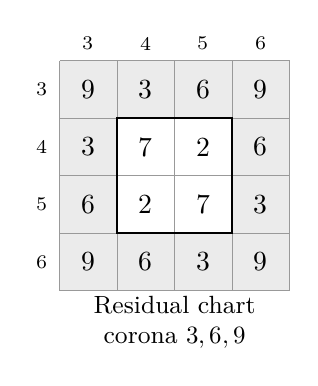
\begin{tikzpicture}[x=.73cm,y=.73cm]
\fill[black!8] (0,0) rectangle (4,4);
\fill[white] (1,1) rectangle (3,3);
\draw[step=1,black!40] (0,0) grid (4,4);
\draw[thick] (1,1) rectangle (3,3);
\foreach \row/\vals in {0/{9,3,6,9},1/{3,7,2,6},2/{6,2,7,3},3/{9,6,3,9}}{
  \foreach \val [count=\col from 0] in \vals{
    \node at (\col+.5,3.5-\row) {\(\val\)};
  }
}
\foreach \v [count=\n from 0] in {3,4,5,6}{
  \node[font=\scriptsize] at (\n+.5,4.3) {\(\v\)};
  \node[font=\scriptsize] at (-.3,3.5-\n) {\(\v\)};
}
\node[font=\small,align=center] at (2,-.55) {Residual chart\\corona \(3,6,9\)};
\end{tikzpicture}
\end{minipage}\hfill
\begin{minipage}[c]{.50\textwidth}
\centering
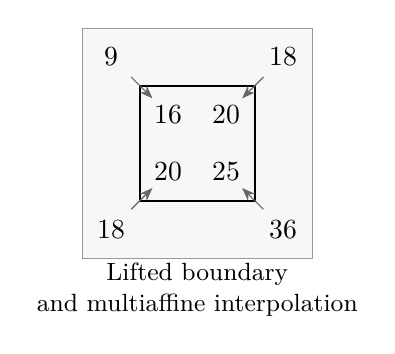
\begin{tikzpicture}[x=.73cm,y=.73cm]
\fill[black!3] (0,0) rectangle (4,4);
\draw[black!40] (0,0) rectangle (4,4);
\draw[thick] (1,1) rectangle (3,3);
\foreach \x/\y/\v in {.5/3.5/9,3.5/3.5/18,.5/.5/18,3.5/.5/36,
  1.5/2.5/16,2.5/2.5/20,1.5/1.5/20,2.5/1.5/25}{
  \node at (\x,\y) {\(\v\)};
}
\draw[-{Stealth},black!60] (.85,3.15) -- (1.22,2.78);
\draw[-{Stealth},black!60] (3.15,3.15) -- (2.78,2.78);
\draw[-{Stealth},black!60] (.85,.85) -- (1.22,1.22);
\draw[-{Stealth},black!60] (3.15,.85) -- (2.78,1.22);
\node[font=\small,align=center] at (2,-.55) {Lifted boundary\\and multiaffine interpolation};
\end{tikzpicture}
\end{minipage}
\caption{The same chart in two readouts. Left: the radical corona surrounds block \(B_c\). Right: the four integer corners determine the interior values under the multiaffine law. Their corner residues coincide, but the quotients \((0,1,1,3)\) distinguish the lift.}
\label{fig:centro-frontera}
\end{figure}


\Needspace{6\baselineskip}
Its inner block is

\[
B_c=\begin{pmatrix}7&2\\2&7\end{pmatrix}.
\]
The perimeter of this chart contains twelve positions: four with value \(3\), four with \(6\), and four with \(9\); their sum is \(72\). A radical crown becomes visible around the central block. The global electronic center is \((5,5)\), the unique fixed point of the inversion of the complete APP; its position does not change upon choosing this local chart, whose geometric center is at \((4.5,4.5)\).

\begin{proposition}[Recovery from the lifted boundary]
\label{prop:centro-frontera-recuperacion}
Let \(F(x,y)=a+bx+cy+dxy\) be a multiaffine law on the chart \([3,6]^2\). For \(t=(x-3)/3\) and \(u=(y-3)/3\),

\[
\begin{aligned}
F(x,y)={}&(1-t)(1-u)F(3,3)+(1-t)uF(3,6)\\
&+t(1-u)F(6,3)+tuF(6,6).
\end{aligned}
\]
\end{proposition}
\begin{proof}
For fixed \(y\), affinity in \(x\) recovers \(F(x,y)\) from \(F(3,y)\) and \(F(6,y)\). Affinity in \(y\) recovers each of these two values from its endpoints. Composition gives the formula. In particular, the four corners determine the entire chart within the declared space of laws.
\end{proof}

For the product, the four lifted values are \(9,18,18,36\). Their positive residues are all \(9\), but their quotients are \(0,1,1,3\). The formula recovers \(16,20,20,25\) at the interior positions; their residual representation gives \(7,2,2,7\). Thus, the boundary determines the interior \textbf{while preserving the law and the lift}. Interpolation is performed before modular reduction: no division by \(3\) is performed in \(\mathbb Z/9\mathbb Z\), where \(3\) is not invertible.

This specifies the meaning of “preserving the information of the center.” The residual crown alone does not individualize all lifts: \(F\) and \(F+9\) have the same residues along the entire boundary and different lifted values. The residue–quotient pair removes that ambiguity within the indicated reconstruction. The assertion is proved for multiaffine laws; extending it to complete states also requires preserving the operators, routes, and memory acting on them.

Multiaffine recovery is a \textbf{new formalization of the preexisting authorial architecture}. The charts and their readouts are results recovered from the corpus; this explicit presentation of their inverse is not credited as an independent historical discovery.

\subsection{Sum, product, and the three values of discrete curvature}
The multiplicative rows are constructed by additive accumulation. The difference between the two sheets appears when both coordinates are varied simultaneously. With unit differences,

\[
\Delta_x\Delta_y(x+y)=0,
\qquad
\Delta_x\Delta_y(xy)=1.
\]
The same property is recovered on the lifted boundary:

\[
\frac{P(6,6)-P(6,3)-P(3,6)+P(3,3)}{3\cdot3}=1;
\]
for \(S(x,y)=x+y\), this quotient equals \(0\). The product records the cross variation that the sum does not introduce. The corpus expresses the oriented version through

\[
\mathcal F(T_x,T_y)=\Delta_x\Delta_yT_y-\Delta_y\Delta_xT_x,
\]
\[
\mathcal F(S,S)=\mathcal F(P,P)=0,
\qquad \mathcal F(S,P)=+1,
\qquad \mathcal F(P,S)=-1.
\]
The order of the sheets distinguishes the sign. The formulation “the sum accumulates and the product folds or unfolds” rests here on a verifiable operation: modular projection preserves a residue; lifting recovers the quotient recording what was exceeded. Discrete curvature additionally records the order of the variations. This finite difference is not identified with a differential curvature of a physical space without its corresponding realization map.

\subsubsection*{The global radical cross}
In \(R=\mathbb Z/9\mathbb Z\), the ideal \(\mathfrak m=\{0,3,6\}\) satisfies \(\mathfrak m^2=0\). Its positive representation is \(\{9,3,6\}\). The cross

\[
(\mathfrak m\times R)\cup(R\times\mathfrak m)
\]
has \(27+27-9=45\) positions. The intersection contains nine values \(9\), summing to \(81\); the remaining arms have twelve values of each class \(3,6,9\), summing to \(216\). The total is

\[
297=216+81=3(72+27)=3\cdot99.
\]
Four boundaries are distinguished: the local perimeter of twelve positions, the radical cross of forty-five, the gnomon of seventeen completing \(8^2\) to \(9^2\), and the cubic crown of \(271\). Each has its own domain and operation. The tritic quotient \(R/\mathfrak m\) preserves a class; transporting the state requires accompanying it with the lifted data and their history.

\subsection{The 72–27 and 77–22 readouts and the 729–271 completion}
The ordered rows of \(B_c\) are expressed decimally as \(72\) and \(27\); its diagonals as \(77\) and \(22\). This gives

\[
72+27=77+22=99.
\]
In the cubic completion, counting the interior, faces, edges, and vertex gives

\[
1000=729+243+27+1=729+271,
\]
\[
999=729+243+27=729+270.
\]
The coincidence of readouts is expressed while preserving the decimal remainder:

\[
729=10\cdot72+9,\qquad271=10\cdot27+1.
\]
Thus, the two-dimensional readout expresses \((72,27)\); the cubic readout expresses \(((72,9),(27,1))\). The pair of remainders \((9,1)\) distinguishes prolongations that would share the same quotient. The chart constructions are performed first; these representations are then compared. Identity of the integers does not reverse that causal order.

The chapter on integer channels provides another specific composition. With the internal counts \(\Delta=54\), \(\nu=\Delta/2=27\), and \(\Theta=5\nu=135\), it obtains

\[
\mathcal C_\alpha=\nu^2=729,
\qquad \mathcal C_e=2\Theta+1=271.
\]
Here \(\nu\) is the new name for the local integer denoted by \(\kappa\) in that source, to distinguish it from the rational readout of the dodecaphase record. The channels are integer objects; their identification with the constants passes through the regional readouts and the corresponding closure, not through the first digits of an expansion. This comparison uses the integer channels and does not require the subsequent angular realization.

For the oral reference to a fraction of \(\pi\), the located source contains

\[
\frac{396}{126}=\frac{22}{7},\qquad
396=18+72+108+198,\quad126=18+108.
\]
This is a rational ratio of alternating rings. This ring ratio is an exact rational readout; its function is distinguished from the regional representation of \(\pi\).

\subsection{The electronic center and its conjugate vacancies}
The inversion of the positive APP is \(\rho(r,c)=(10-r,10-c)\). Its unique fixed point is \((5,5)\). In the central additive fiber,

\[
\mathcal F_{10}=\{(5+t,5-t):t\in\mathbb Z,\ |t|\leq4\},
\]
the product equals \(25-t^2\). Preserving its central residue requires \(t^2\equiv0\pmod9\), equivalent to \(3\mid t\). The only positions are therefore

\[
(5,5),\qquad(8,2),\qquad(2,8).
\]
If \(\mathcal A\) preserves the residue–quotient pair on each sheet,

\[
\begin{aligned}
\mathcal A(5,5)&=((1,1),(7,2)),\\
\mathcal A(8,2)=\mathcal A(2,8)&=((1,1),(7,1)).
\end{aligned}
\]
The two vacancies preserve the additive readout and the multiplicative residue; the product quotient decreases by exactly one unit. The mirror \(t\mapsto-t\) exchanges their positions. The residual value does not distinguish their routes, whereas orientation does preserve them. This is a precise realization of the connection indicated in the note: \textbf{a vacancy is individualized by a relation to the center and by a recorded defect, not by being a cell without information}.

The initial electronic orientation \((h_0,v_0)=(1,1)\), reversed every \(27\) steps, subsequently expresses the dodecaphase signature \((+++\,---\,+++\,---)\). This is an orientation record, distinct both from the position \((5,5)\) and from the product signature below.

\subsubsection*{The signature 555555 and the memory enabling its prolongation}
For \(U_j=100d_{1j}+10d_{2j}+d_{3j}\), the readout

\[
\mathcal E_\times(U)=([d_{2j}-d_{1j}]_{10})_{j=1}^{6}
\]
applied to the transverse region

\[
U_\pi^\perp=(501,614,498,169,272,272)
\]
produces \(555555\); its reduction \(\Psi(U)=(-U_j\bmod3)_j\) produces \(010211\). The signature has twenty-four product representatives. Transport separates them into three sheets of eight: after advancement, \(555177\), \(555717\), and \(555771\) appear. The congruence stable under advancement and half-turn refines the twenty-six signatures into twenty-eight classes, with histogram \(27\cdot8+108=324\). This expresses why sheet memory must be retained to continue a signature that initially coincides.

\begin{definition}[Signature readout and transport of representatives]
\label{def:firma555}
Let \(\mathcal X_\times=D_9^2\times\{N,E,S,O\}\), of cardinality \(324\).
Advancement \(P\) moves one cell in the stored direction, and the half-turn
\(H\) reverses that direction. The readout uses
\[
\ell_9(1,2,4,8,7,5)=(0,1,2,3,4,5),\qquad
\ell_9(3)=\ell_9(6)=\ell_9(9)=0.
\]
In each of six windows of nine steps,
\(\ell_9(\rho_9(ij))\) is evaluated before the product advancement selected by TRIT at
times \(2,5,8\pmod9\). The sum in each window is reduced modulo
\(10\). After steps \(27\) and \(54\), the direction is reversed.
The rule determines \(E_{\rm sig}(x)\) from the position and direction
of \(x\), with the kernel's time conventions.
\end{definition}

\begin{proposition}[Minimal stable refinement of the signature]
\label{prop:firma555}
Starting from equivalence by signature \(\sim_0\), the iteration
\[
x\sim_{n+1}y\ \Longleftrightarrow\
x\sim_n y,\quad Px\sim_n Py,\quad Hx\sim_n Hy
\]
terminates and produces the coarsest stable congruence refining the signature.
On the preceding domain the census is \(26\to28\to28\); the fiber of
\(555555\) separates into three classes of eight representatives.
\end{proposition}
\begin{proof}
At each step, a partition of a finite set is refined. The process
stabilizes after finitely many splittings. At the fixed point,
equivalence is preserved under \(P\) and \(H\). If a stable congruence
refines \(\sim_0\), it refines each \(\sim_n\) by induction: its images
under both operators remain equivalent. It therefore refines the fixed
point obtained, proving its minimality in added information.

The finite enumeration applies the definition to the \(81\) positions and the
four orientations. Their six sums modulo \(10\) are grouped first, and
then the triple consisting of the class of \(x\), that of \(Px\), and that of
\(Hx\), until stabilization. The resulting histogram is
\(27\cdot8+108=324\), and the only signature splitting is the one indicated.
The following representatives make the three images explicit:
\[
\begin{array}{c|c|c}
x&E_{\rm sig}(x)&E_{\rm sig}(Px)\\\hline
(3,5,N)&555555&555177\\
(3,4,N)&555555&555717\\
(3,4,S)&555555&555771
\end{array}
\]
The complete rule and its executable enumeration are preserved in the
reproduction package; the witnesses in the table also show that preserving
only the signature does not make its continuation unique.
\end{proof}

The conclusion describes the minimal information of transport, not a
new mass. The additive factor preserves eighteen representatives per signature
(nine compatible positions and two orientations). Combining it with the
product fibers of sizes \(24\) and \(8\) gives, respectively,
\(432\) and \(144\). Regional incidence and sheet memory thus preserve
distinct functions within the same catalog.


The link to the electronic equation passes through the regions. The transverse region has multiplicity \(432=18\cdot24\); each of the other four has \(144=18\cdot8\). Their five identities are inserted, in the declared gauge of Article I, into

\[
\mathcal K_e=\mathbb Z/9\mathbb Z\times\mathbb F_3
\]
through \((4,0),(5,0),(6,0),(6,1),(6,2)\). Once this insertion has been fixed, its complement has \(27-5=22\) positions and its three sheets per region have \(5\cdot3=15\) positions. The oriented deficit and torsional memory are \(-22\) and \(15\). The proof of these counts follows from the preceding explicit injection: its five images are distinct; this development brings it together, rather than selecting its positions from a target mass.

There are therefore two linked progressions in the composition: \textbf{center → conjugate vacancies → orientation}, and \textbf{regional signature → transport sheets → incidence of the five regions → electronic coefficients}. Simply identifying \((5,5)\) with \(555555\) would erase precisely the operations explaining their relation.

\subsection{Nonadic mirror, capacity, and return with memory}
On the regional fiber, the mirror acts by

\[
\mathfrak c(u^\pi,u^e,u^\varphi)=(u^e,u^\pi,u^\varphi).
\]
It preserves \(s=u^\pi+u^e\) and reverses \(d=u^\pi-u^e\). In \(\mathbb F_3\),

\[
u^\pi=2(s+d),\qquad u^e=2(s-d).
\]
The sum preserves the aggregate; the oriented difference preserves its distribution. The axis \(u^\varphi\) remains fixed under this involution, although it may evolve under transport. The regional mirror and the cellular mirror of the vacancies have different domains: their respective formulas make it possible to track what each preserves.

The capacity vacancy adds an explicit temporal link. In the normalization of refinement \(729\) versus \(1000\), let \(\rho_c=\log_{10}9\), \(\delta=1-\rho_c\), and \(\mathcal C_t=\lfloor(t+1)\rho_c\rfloor\). If

\[
z_t=\lfloor(t+1)\delta\rfloor-\lfloor t\delta\rfloor,
\]
then, for \(t\geq1\),

\[
\mathcal C_t-\mathcal C_{t-1}=1-z_t,
\qquad
\mathcal C_b-\mathcal C_a+\sum_{t=a+1}^b z_t=b-a.
\]
\begin{proof}
The irrationality of \(\log_{10}9\) follows from the impossibility of \(9^n=10^m\) for positive integers. Hence, \(\mathcal C_t=t-\lfloor(t+1)\delta\rfloor\). Subtraction and telescoping summation give both identities. \end{proof}
A vacancy retains capacity while the history advances.

If \(p_j=\lfloor j/\delta\rfloor\), \(v_j=p_j-j\), and \(h_j=p_{j+1}-p_j\), the inherited development establishes \(h_j\in\{21,22\}\). For \(s_j=22-h_j\),

\[
[v_{j+1}]_3=[v_j-s_j]_3,\qquad
\tau_j=M_{\rm ph}(1+[v_j]_9).
\]
Vacancies thus act on the retained phase read by the tritic selector. This capacity sequence does not automatically become the electron's cellular trajectory: the manuscript preserves their respective mechanisms and their composition within the same kernel.

% RESULTADO_RECUPERADO and expanded self-contained exposition; the common kernel is unchanged.
% Compared source owners:
% Article I REV02/sections/vacancias_capacidad.tex, complete.
% Monografia775/manuscrito/generated/cristal_relojes_sincronizacion.tex,
% lines1--223 and931--1032: capacity, returns, and TRIT induction.
% The universal proofs of both scales are assembled here; the checker
% ampliacion/verificar_vacancias.py adds a finite rational certificate.
\subsection{Vacancies of nonadic refinement and hierarchy of returns}
\label{vac-add-seccion}

APP--TRIT--TPK prolongation preserves, together with the expressed block, the cylinder, orientation, and history that allow it to be continued. Its capacity readout compares two cardinalities already determined by that construction: the \(3^6=729\) possibilities of a six-position ternary block and the \(10^3=1000\) positions of its three-digit decimal chart. This comparison produces its own schedule. Some transitions increase the capacity index; others incorporate a block into the history while retaining that index. The latter are the \emph{capacity vacancies} studied below.

The object under consideration is therefore a representation of joint refinement. Its definition preserves its origin in the two finite supports; the logarithmic expression permits the properties of its schedule to be proved. Block time, vacancy index, and capacity index will be written separately. This separation makes clear why the returns \(21/22\) and \(6/7\) belong to successive scales of a single construction.

\subsubsection{Decimal capacity and preservation of the increment}
\label{vac-add-capacidad}

\begin{definition}[Capacity index and vacancy]
\label{vac-add-definicion}
At phase origin \(0\), define
\begin{equation}
 \rho=\log_{1000}729=\log_{10}9,
 \qquad \delta=1-\rho=\log_{10}(10/9),
 \label{vac-add-densidad}
\end{equation}
and, for \(t\in\mathbb Z_{\geq0}\),
\begin{equation}
 \mathcal C_t=\lfloor(t+1)\rho\rfloor,
 \qquad
 z_t=\lfloor(t+1)\delta\rfloor-\lfloor t\delta\rfloor.
 \label{vac-add-indices}
\end{equation}
The integer \(\mathcal C_t\) is the decimal capacity index of the readout; \(z_t=1\) marks a vacancy. The letter \(K\) remains reserved for the dodecaphasic register and does not denote a capacity counter here.
\end{definition}

We have \(0<\delta<1\). Moreover, \(\delta\) is irrational: if \(\rho=a/b\) were rational, with \(a,b\) positive integers, the equality \(9^b=10^a\) would have zero valuation at the prime \(5\) on the left and positive valuation on the right. This contradiction proves the irrationality of \(\rho\) and of \(1-\rho\). In particular, no positive integer multiple of \(\delta\) belongs to \(\mathbb Z\), which fixes the endpoints of the intervals in this development unambiguously.

\begin{proposition}[Exact capacity--vacancy balance]
\label{vac-add-balance}
For \(t\geq1\), \(z_t\in\{0,1\}\) and
\begin{equation}
 \mathcal C_t-\mathcal C_{t-1}=1-z_t.
 \label{vac-add-incremento}
\end{equation}
Consequently, for \(0\leq a<b\),
\begin{equation}
 \mathcal C_b-\mathcal C_a+
 \sum_{t=a+1}^{b}z_t=b-a.
 \label{vac-add-conservacion}
\end{equation}
\end{proposition}
\begin{proof}
Since \(0<\delta<1\), the difference between the floors of two numbers separated by \(\delta\) is \(0\) or \(1\). Furthermore, the established irrationality gives
\[
 \mathcal C_t=t+1-\lceil(t+1)\delta\rceil
             =t-\lfloor(t+1)\delta\rfloor.
\]
Subtracting this equality at \(t\) and \(t-1\) proves \eqref{vac-add-incremento}; telescopic summation proves \eqref{vac-add-conservacion}.
\end{proof}

Each transition contributes exactly one unit to the right-hand side of the balance. That unit is recorded as acquired capacity when \(z_t=0\), or as a vacancy when \(z_t=1\). Retention of the index \(\mathcal C_t\) therefore leaves a recoverable position in the history. The equation expresses preservation of the increment through two readouts, rather than an indeterminate loss of information.

The density also follows from the same balance:
\[
 \frac1N\sum_{t=1}^{N}z_t
 =\frac{\lfloor(N+1)\delta\rfloor}{N}\longrightarrow\delta.
\]
Thus \((z_t)\) is not eventually periodic: an eventually periodic binary sequence has rational density. Here aperiodicity follows from the capacity rule already fixed by \(729/1000\).

\subsubsection{Exact determination of the intervals \(21/22\)}
\label{vac-add-primarios}

\begin{lemma}[Rational bounds for the slope]
\label{vac-add-cotas}
The vacancy density satisfies
\begin{equation}
 \frac7{153}<\delta<\frac6{131}.
 \label{vac-add-cota-delta}
\end{equation}
If \(\lambda=\delta^{-1}\), \(\beta=22-\lambda\), and \(\mu=\beta^{-1}\), then
\begin{equation}
 21<\lambda<22,
 \qquad \frac17<\beta<\frac16,
 \qquad 6<\mu<7.
 \label{vac-add-cotas-inducidas}
\end{equation}
\end{lemma}
\begin{proof}
We provide a finite verification by rational arithmetic. For \(0<u<1\), let
\[
 S_N(u)=2\sum_{k=0}^{N}\frac{u^{2k+1}}{2k+1},
 \qquad
 R_N(u)=\frac{2u^{2N+3}}{(2N+3)(1-u^2)}.
\]
Integrating the geometric series for \(2/(1-u^2)\) gives
\[
 S_N(u)<\log\frac{1+u}{1-u}<S_N(u)+R_N(u).
\]
Indeed, the tail is positive and, on replacing each denominator \(2k+1\) by \(2N+3\), is bounded by the geometric series defining \(R_N\). These inequalities are applied to \(u=1/19,1/3,1/9\), corresponding respectively to \(\log(10/9),\log2,\log(5/4)\), and we use \(\log10=3\log2+\log(5/4)\).

With \(N=4\), writing \(A=S_4(1/19)\), \(B=3S_4(1/3)+S_4(1/9)\), and \(E=3R_4(1/3)+R_4(1/9)\), we obtain
\[
 \frac7{153}
 <\frac{A}{B+E}
 <\delta
 <\frac{A+R_4(1/19)}{B}
 <\frac6{131}.
\]
The two outer inequalities are checked by multiplying through by the positive denominators of these sums of five rational terms. This proves \eqref{vac-add-cota-delta} using a remainder bound, without taking a decimal expansion as a premise. Inverting the bound gives \(131/6<\lambda<153/7\). Subtracting from \(22\) and then inverting yields all the inequalities in \eqref{vac-add-cotas-inducidas}.
\end{proof}

\begin{theorem}[Positions and gaps of the vacancies]
\label{vac-add-teorema-primario}
The positions of the events \(z_t=1\), ordered from the first event, are exactly
\begin{equation}
 p_j=\lfloor j\lambda\rfloor
     =\left\lfloor\frac j\delta\right\rfloor,
 \qquad j\geq1.
 \label{vac-add-posiciones}
\end{equation}
Their gaps satisfy
\begin{equation}
 h_j=p_{j+1}-p_j\in\{21,22\}.
 \label{vac-add-huecos}
\end{equation}
Both values occur infinitely often.
\end{theorem}
\begin{proof}
The event crossing the integer \(j\) occurs precisely when \(t\delta<j<(t+1)\delta\). Irrationality excludes equality at the endpoints. Dividing by \(\delta\) gives \(t=\lfloor j/\delta\rfloor=p_j\). Since \(\delta<1\), a step crosses at most one integer, so the enumeration is exact. Writing \(\lambda=21+\eta\), with \(0<\eta<1\), gives
\[
 h_j=21+\lfloor(j+1)\eta\rfloor-\lfloor j\eta\rfloor,
\]
which proves \eqref{vac-add-huecos}. Finally, \((p_{J+1}-p_1)/J\to\lambda\in(21,22)\). If either value occurred only finitely often, this mean would converge to the other integer value, a contradiction.
\end{proof}

\subsubsection{Induction on the short intervals: the returns \(6/7\)}
\label{vac-add-secundarios}

\begin{theorem}[Induced schedule of short intervals]
\label{vac-add-teorema-secundario}
Let \(s_j=22-h_j\), for \(j\geq1\). This indicator equals \(1\) exactly when the interval between vacancies is short, of length \(21\). With \(\beta\) and \(\mu\) as defined in Lemma~\ref{vac-add-cotas},
\begin{equation}
 s_j=\lfloor(j+1)\beta\rfloor-\lfloor j\beta\rfloor.
 \label{vac-add-indicador-corto}
\end{equation}
The indices of the short intervals are
\begin{equation}
 q_m=\lfloor m\mu\rfloor=\lfloor m/\beta\rfloor,
 \qquad q_{m+1}-q_m\in\{6,7\},\quad m\geq1.
 \label{vac-add-posiciones-cortos}
\end{equation}
Both gaps occur infinitely often, and their order is not eventually periodic.
\end{theorem}
\begin{proof}
The irrationality of \(\delta\) implies that of \(\lambda\), \(\beta\), and \(\mu\). Since \(\lambda=22-\beta\), for \(j\geq1\) we have
\[
 p_j=22j-\lceil j\beta\rceil
     =22j-\lfloor j\beta\rfloor-1.
\]
Subtracting consecutive terms gives \eqref{vac-add-indicador-corto}. Applying the integer-crossing argument of the preceding theorem to the indicator of slope \(\beta\) shows that its event \(m\) occurs at \(q_m=\lfloor m/\beta\rfloor\). The inequality \(6<\mu<7\) proves the two possible gaps. Their mean converges to \(\mu\); hence both occur infinitely often. Moreover, an eventually periodic sequence of gaps would have rational mean, whereas \(\mu\) is irrational. This also rules out strict alternation, whose mean would be \(13/2\).
\end{proof}

Here the numbers \(6\) and \(7\) count \emph{intervals between vacancy events}, not refinement blocks. The return to the primary scale is equally explicit. Between \(q_m\) and \(q_{m+1}\) there is a single short interval, located at the beginning, and all the others are long. Consequently, if \(d_m=q_{m+1}-q_m\),
\begin{equation}
 p_{q_{m+1}}-p_{q_m}=21+22(d_m-1)=22d_m-1
 \in\{131,153\}.
 \label{vac-add-retorno-bloques}
\end{equation}
Thus \(131=14\cdot9+5\) and \(153=17\cdot9\) describe two return readouts \emph{in the block clock}. The equation preserves the operation connecting the scales, rather than identifying their cardinalities merely because they occur.

\subsubsection{Retained capacity and selection of the TRIT regime}
\label{vac-add-regimen}

Let \(v_j=\mathcal C_{p_j}\) be the capacity recorded at vacancy \(j\). From \(p_j\delta<j<(p_j+1)\delta\) and \(\delta<1\), it follows that \(\lfloor(p_j+1)\delta\rfloor=j\). By \eqref{vac-add-indices},
\begin{equation}
 v_j=p_j-j,
 \qquad v_{j+1}-v_j=h_j-1=21-s_j,
 \qquad [v_{j+1}]_3=[v_j-s_j]_3.
 \label{vac-add-transporte-mod3}
\end{equation}
A long interval preserves the class modulo \(3\); a short interval shifts it by one unit in the negative direction. Applying the selector of the formal kernel to the positive phase \(r_j=1+[v_j]_9\) gives
\begin{equation}
 \tau_j=M_{\rm ph}(r_j),\qquad
 M_{\rm ph}(r)=
 \begin{cases}
 +1,&r\in\{1,4,7\},\\
 -1,&r\in\{2,5,8\},\\
 0,&r\in\{3,6,9\}.
 \end{cases}
 \label{vac-add-selector}
\end{equation}
This composition fixes the regime induced by capacity at each event. It preserves both the order of the changes and the number of events for which each regime persists.

\begin{corollary}[Plateaus of the induced regime]
\label{vac-add-mesetas}
For every \(m\geq1\), the class \([v_j]_3\), and hence \(\tau_j\), is constant on \(q_m+1\leq j\leq q_{m+1}\). The length of each complete plateau is \(q_{m+1}-q_m\in\{6,7\}\).
\end{corollary}
\begin{proof}
On the indicated integer interval, the next change occurs exactly when passing from \(j=q_{m+1}\) to \(j=q_{m+1}+1\): this is the next position at which \(s_j=1\). At all preceding steps \(s_j=0\), so \eqref{vac-add-transporte-mod3} preserves the class. At the endpoint it decreases the class by one unit. The selector \eqref{vac-add-selector} assigns distinct values to the three classes; it therefore preserves the same plateaus and their endpoints.
\end{proof}

The initial segment \(1\leq j\leq q_1\) depends on the chosen origin and is an initial restriction of a plateau. At the present origin it has length \(q_1=6\). The first twenty classes are
\[
 \underbrace{2,\ldots,2}_{6},\qquad
 \underbrace{1,\ldots,1}_{7},\qquad
 \underbrace{0,\ldots,0}_{7},
\]
with signatures \(0,-1,+1\), respectively. Each short interval triggers the next step of the cycle of regimes.

The two phases of interest are defined as
\[
 g_t^{\rm cron}=[t]_9,
 \qquad g_t^{\rm cap}=[\mathcal C_t]_9,
 \qquad
 g_t^{\rm cap}-g_{t-1}^{\rm cap}\equiv1-z_t\pmod9.
\]
A vacancy retains the capacity phase while block time advances. The transition of the enriched state remains the TPK composition of selection, transport, and memory update. Thus \(\mathcal C_t=\mathcal C_{t-1}\) neither resets the state nor replaces the holonomic winding \(\Gamma_9\) by a pause. The two induced scales likewise retain this distinction: between consecutive short events in \eqref{vac-add-retorno-bloques}, the capacity increment is \(21d_m-1\), that is, \(125\) or \(146\), whereas the block increment is \(131\) or \(153\).

\subsubsection{Rationally certified sample and provenance}
\label{vac-add-muestra}

The table presents a sample at the canonical origin. \(h_j\) is the gap \emph{following} \(p_j\); thus vacancy \(j=6\), at block \(131\), begins the first short interval.
\begin{center}
\small
\begin{tabular}{r|rrrrrrrrrr}
\toprule
\(j\)&1&2&3&4&5&6&7&8&9&10\\
\midrule
\(p_j\)&21&43&65&87&109&131&152&174&196&218\\
\(h_j\)&22&22&22&22&22&21&22&22&22&22\\
\(v_j\)&20&41&62&83&104&125&145&166&187&208\\
\([v_j]_3\)&2&2&2&2&2&2&1&1&1&1\\
\bottomrule
\end{tabular}
\end{center}
The first short-interval indices and their gaps are
\[
 (q_m)_{m=1}^{10}=(6,13,20,27,34,41,48,54,61,68),
\]
\[
 (q_{m+1}-q_m)_{m=1}^{9}=(7,7,7,7,7,7,6,7,7).
\]
The sample exhibits the actual order, while the preceding proofs establish its law at arbitrary depth.

The attached file \texttt{ampliacion/verificar\_vacancias.py} computes rational brackets using the series and remainders of Lemma~\ref{vac-add-cotas}. Each floor is accepted only when both endpoints of the bracket yield the same integer. At order \(16\), it reproduces \(512\) events up to block \(11189\), and \(64\) secondary gaps, together with the balance identities, residues, and plateaus. This finite check retains a scope distinct from that of the universal theorems.

The capacity index, its complementarity with vacancies, and induction of the TRIT selector are recovered from Article I and from the chapters on the schedule and induced clock in the monograph on aperiodic topological--temporal order. Their definitions and the proofs of both scales are assembled here with a single indexing convention. The rational certificate provides an additional check of those results and preserves their provenance.


\subsection{The factor 8/81 as a balance between representation and complement}
In the double-circle development, the uniform inclusion of nine phases is \(Jv=(v,\ldots,v)/3\). With the seam

\[
S_C(v_0,\ldots,v_8)=(Cv_8,v_0,\ldots,v_7),
\]
one obtains \(T=J^*S_CJ=(8I+C)/9\). If \(z=(C-I)v\), the complement of the representation is exactly

\[
\eta v=(I-JJ^*)S_CJv=\frac1{27}(8z,-z,\ldots,-z).
\]
Hence,

\[
\|\eta v\|^2=\frac{64+8}{729}\|z\|^2
=\frac8{81}\|(C-I)v\|^2.
\]
Here appears the \(8/81\) mentioned by the author: one transported phase against eight others, with the uniform normalization of nine phases. The result does not depend on which of the nine positions is marked. The complete operator balance is

\[
I-T^*T=\frac8{81}(I-C)^*(I-C)+\frac19(I-C^*C).
\]
If \(C\) is isometric, the energy omitted by representation lies exactly in its complement. For an arbitrary seam, its explicit defect is also preserved. The integer \(72=64+8\) counts quadratic weights here; in the local crown it counts a sum of values; in \(72/27\) it belongs to an ordered decimal readout. Specifying these types makes it possible to relate the constructions without assuming that a numerical coincidence already provides all maps between them.

This balance remains that of the double-circle transport development. When applied to the arithmetic form \(\mathscr W\), it produces a signed identity; proving global positivity requires global control of its terms, not merely recovery of the center or positivity of an auxiliary norm. The results already proved concerning memory, transport, and the coercive window are preserved in full.

\clearpage
\section{Native product, factorization, and irreducibility}
\label{lectura:manuscrito-01}
This chapter develops the arithmetic sector of normal forms over the common kernel and the correlative construction of the continuum in Section~\ref{lectura:manuscrito-05}. The local operation extends to words, its fibers distinguish the irreducibles, and evaluation makes it possible to recognize the primes. The development recovers the native product of the corpus; its documentary provenance is collected in Appendix~\ref{ap:procedencia-reproduccion}.

\subsection{The information required for multiplication}
Selecting prime numbers requires a multiplication to have been constructed. In Triadic Modular Holography, this operation must be presented from the two APP sheets, preserving both the residual coordinate and its quotient. The residue alone makes it possible to recognize a congruence class. The residue–quotient pair makes it possible to reconstruct the integer result of the local operation. This distinction determines which information must be transported when composing the cells.

Let $D_9=\{1,\ldots,9\}$. For each pair $(a,b)\in D_9^2$, the additive and multiplicative sheets are written as

\[
a+b=R_+(a,b)+9Q_+(a,b),\qquad
ab=R_\times(a,b)+9Q_\times(a,b),
\]
with $R_+,R_\times\in D_9$. The choice of the positive representative uniquely fixes the four data. In particular, a result divisible by nine has its residue represented by $9$, and its quotient is one less than that of Euclidean division with zero remainder. This is an exact representation convention, which must be maintained throughout the construction.

For example,

\[
2\cdot5=1+9\cdot1,\qquad 9\cdot9=9+9\cdot8.
\]
The first result preserves the information that distinguishes $10$ from $1$; the second preserves that which distinguishes $81$ from $9$. If the quotient is omitted at one of these steps, a subsequent multiplication acts on a different object. Arithmetic memory here is not an interpretation added to the algorithm: it participates in reconstructing its result.

The two sheets are coupled even during multiplication. The product of two digits generates a pair $(R_\times,Q_\times)$; when the quotient from a preceding position is incorporated into the current position, the additive sheet is needed again. The global operation composes both sheets.

\HMTresultado{Proposition}{Local compatibility of the quotients}{rz-num-01-1}
The quotients satisfy the identities required to associate and distribute the operations without changing the reconstructed integer. For example, for addition,

\[
Q_+(a,b)+Q_+\bigl(R_+(a,b),c\bigr)
=Q_+(b,c)+Q_+\bigl(a,R_+(b,c)\bigr).
\]
For multiplication,

\[
Q_\times\bigl(R_\times(a,b),c\bigr)+cQ_\times(a,b)
=Q_\times\bigl(a,R_\times(b,c)\bigr)+aQ_\times(b,c).
\]
\textbf{Proof.} Substituting the two decompositions of $a+b+c$, the final residues are the same positive representative of its class modulo nine. Subtracting them and dividing by nine gives the first equality. For $abc$, the same argument is applied to

\[
\bigl(R_\times(a,b)+9Q_\times(a,b)\bigr)c
=a\bigl(R_\times(b,c)+9Q_\times(b,c)\bigr).
\]
The distributive identity is obtained by reconstructing $a(b+c)=ab+ac$ with the two sheets. In all three cases, uniqueness of the residual representation determines exactly the quotient that must accompany it. \hfill\(\square\)

These identities make it possible to organize the operation record: two parenthesizations produce the same integer without requiring their execution histories to be identified. Equality of the result and identity of the history are different assertions.

\subsection{Nonadic words and normal form}
The extension to arbitrarily large integers uses finite sequences of digits from $D_9$. The orientation adopted runs from the least significant to the most significant position. For $u=(u_0,\ldots,u_{r-1})$, let

\[
\operatorname{ev}_9(u)=\sum_{j=0}^{r-1}u_j9^j.
\]
The empty sequence represents zero. In this bijective numeration, the symbol $9$ remains a digit; it does not become a zero without a quotient.

\HMTresultado{Proposition}{Existence and uniqueness of the normal form}{rz-num-01-2}
The preceding evaluation is a bijection between finite words over $D_9$, including the empty word, and nonnegative integers.

\textbf{Proof.} If $n>0$, define

\[
d(n)=1+((n-1)\bmod9),\qquad q(n)=\frac{n-d(n)}9.
\]
Then $d(n)\in D_9$, $q(n)\ge0$, and $q(n)<n$. Iteration terminates at zero and produces a word whose evaluation is $n$. For uniqueness, the first digit of any word evaluating to $n$ must represent the class of $n$ modulo nine within $D_9$; it must therefore be $d(n)$. Removing it and dividing by nine reduces the question to $q(n)$. Induction proves uniqueness. \hfill\(\square\)

Some normal forms are

\[
9\leftrightarrow(9),\quad
10\leftrightarrow(1,1),\quad
81\leftrightarrow(9,8),\quad
1000\leftrightarrow(1,3,3,1).
\]
The representation is checked directly: $1000=1+3\cdot9+3\cdot9^2+9^3$. This last equality does not by itself identify the word of an integer with the cubic completion of a geometric domain. The two occurrences of $1000$ have different objects and operations; an identification would require its map.

The normal form is an arithmetic coordinate. The TPK state additionally preserves orientation, sheet, route, boundary, and transport memory. When different histories produce the same normal form, the evaluation map brings their values together, but does not establish a bijection between those histories. The development of the article must preserve both levels and the map relating them.

\subsection{Construction of the product without prior evaluation of the operands}
Word addition is performed position by position. If a position contains two digits, the additive sheet is consulted. If it contains only one, that digit is retained. The quotient arriving from the preceding position is incorporated through another additive lookup, and the quotients of both lookups are added. If \(a+b=r+9q\) and \(r+c=r'+9q'\), then \(q+q'\) is transported. For example, \(9+9+1=1+9\cdot2\). The incoming quotient lies between zero and two; when it is zero, no additional cell is consulted. An absent position is not an APP cell containing the digit zero.

Multiplication by a digit $d\in D_9$ acts analogously: at each position, the multiplicative sheet is first applied to the digit of the word and to $d$; the pending quotient is then incorporated through the additive sheet. The new quotient is the sum of the quotient of the local product and that of this additive lookup, and lies between zero and nine. The procedure terminates by appending the final quotient when it is nonzero.

Denote these operations by $u\boxplus v$ and $d\odot u$. If $v=(v_0,\ldots,v_{m-1})$, the native product is constructed through the recurrence

\[
a_m=\varnothing,\qquad
a_j=(9\odot a_{j+1})\boxplus(v_j\odot u),
\quad j=m-1,\ldots,0,
\]
and $u\boxtimes v=a_0$ is defined. Every operation on the right-hand side uses the two local sheets already defined. Word evaluation does not intervene as an instruction for computing the product.

\HMTresultado{Theorem}{Exactness of the native product}{rz-num-01-3}
For all finite words $u,v$,

\[
\operatorname{ev}_9(u\boxtimes v)
=\operatorname{ev}_9(u)\operatorname{ev}_9(v).
\]
\textbf{Proof.} The cell reconstruction identities prove, by induction over positions, that

\[
\operatorname{ev}_9(u\boxplus v)
=\operatorname{ev}_9(u)+\operatorname{ev}_9(v),\qquad
\operatorname{ev}_9(d\odot u)=d\operatorname{ev}_9(u).
\]
The product recurrence preserves the invariant

\[
\operatorname{ev}_9(a_j)
=\operatorname{ev}_9(u)\sum_{k=j}^{m-1}v_k9^{k-j}.
\]
The case $j=m$ is immediate. If it holds for $j+1$, multiplying by nine and adding $v_j\operatorname{ev}_9(u)$ yields the case $j$. For $j=0$, the asserted equality follows. \hfill\(\square\)

\HMTresultado{Corollary}{Multiplicative structure of the normal forms}{rz-num-01-4}
The nonempty words, with the product $\boxtimes$, form a commutative monoid whose unit is $(1)$. Upon adjoining the empty word, it is absorbing.

\textbf{Proof.} Evaluation is multiplicative by the theorem and injective by Proposition~\ref{rz-num-01-2}. Associativity, commutativity, and the identity are verified after evaluation and recovered by injectivity. \hfill\(\square\)

The proof makes it possible to recognize ordinary multiplication in the constructed operation. The logical order matters: the cell transducer is first defined and its invariant is proved; its integer realization is then identified.

\subsection{Multiplicative openings and selection of irreducibles}
Once the product has been constructed, factorization can be defined as its fiber. For each nonempty word $w$, let

\[
\operatorname{Fac}(w)=\{(u,v):u\boxtimes v=w\}.
\]
This fiber is finite. Indeed, if $n=\operatorname{ev}_9(w)$, exactness implies $\operatorname{ev}_9(u)\operatorname{ev}_9(v)=n$, with both factors positive and no greater than $n$. Finiteness justifies the algebraic sum

\[
\Delta e_w=\sum_{(u,v)\in\operatorname{Fac}(w)}e_u\otimes e_v.
\]
The order in the factor pair is preserved. For $n=12$, for example, the evaluations of the fiber are

\[
(1,12),(2,6),(3,4),(4,3),(6,2),(12,1).
\]
The reduced coproduct removes the two decompositions containing the unit, for $w\ne(1)$:

\[
\widetilde\Delta e_w
=\sum_{\substack{u\boxtimes v=w\\u\ne(1),\ v\ne(1)}}e_u\otimes e_v.
\]
Set $\widetilde\Delta e_{(1)}=0$. This convention allows the unit to be treated separately, without confusing it with an irreducible.

\HMTresultado{Definition}{Native irreducible}{rz-num-01-5}
A word $w\ne(1)$ is multiplicatively irreducible if $\widetilde\Delta e_w=0$.

The definition receives no table of primes and uses no decimal period. It asks whether the operation already constructed admits a nontrivial opening.

\HMTresultado{Theorem}{Recognition of the primes}{rz-num-01-6}
Evaluation establishes a bijection between native irreducibles and positive prime numbers.

\textbf{Proof.} If $w=u\boxtimes v$ with factors different from the unit, its evaluation is the product of two integers greater than one; it is therefore not prime. Conversely, if $\operatorname{ev}_9(w)=ab$, with $a,b>1$, their normal forms $u,v$ satisfy

\[
\operatorname{ev}_9(u\boxtimes v)=ab=\operatorname{ev}_9(w).
\]
Injectivity gives $u\boxtimes v=w$, so that $w$ is not irreducible. The bijection of normal forms completes the proof. \hfill\(\square\)

This result identifies a property of the operation with the property of its integer realization. Prime values appear upon evaluating the selected objects, after the product and its fibers have been defined.

\HMTresultado{Proposition}{Coassociativity}{rz-num-01-7}
On the algebraic space generated by positive words,

\[
(\Delta\otimes I)\Delta=(I\otimes\Delta)\Delta.
\]
\textbf{Proof.} Both sides enumerate, with coefficient one, the ordered triples $(u,v,z)$ whose product is $w$. Associativity of the product identifies the two parenthesizations, and all sums are finite. \hfill\(\square\)

\subsection{Operator realization of the selector}
In \(\mathcal H=\ell^2(\mathcal W_9^+)\), with orthonormal basis \(\{e_w\}\), the coproduct is first defined on finite linear combinations. The supports of $\Delta e_w$ and $\Delta e_{w'}$ are disjoint if $w\ne w'$: an ordered pair has a unique product. Hence,

\[
\|\Delta e_w\|^2=|\operatorname{Fac}(w)|,
\qquad
\|\widetilde\Delta e_w\|^2=r(w),
\]
where $r(w)$ counts the ordered nontrivial openings.

The closure of $\widetilde\Delta$ has domain

\[
\left\{x=\sum_wx_we_w\in\mathcal H:\sum_wr(w)|x_w|^2<\infty\right\}.
\]
Its associated positive operator is diagonal:

\[
A_{\mathrm{irr}}=\overline{\widetilde\Delta}^{\,*}\overline{\widetilde\Delta},
\qquad A_{\mathrm{irr}}e_w=r(w)e_w.
\]
Its maximal domain is

\[
\operatorname{Dom}(A_{\mathrm{irr}})
=\left\{x\in\mathcal H:\sum_wr(w)^2|x_w|^2<\infty\right\}.
\]
The projector onto the irreducibles is then

\[
P_{\mathrm{irr}}=(I-P_{(1)})\mathbf1_{\{0\}}(A_{\mathrm{irr}}).
\]
The formula incorporates two distinct exclusions: the kernel removes all words possessing a nontrivial opening, and $I-P_{(1)}$ removes the unit. Positivity comes from a squared norm and has a specific meaning here: it counts decompositions. It is not yet an assertion about the positivity of another form, such as the completed Weil form.

\subsection{Normalized readout of the TPK prefix and preservation of genealogy}
The normal form admits an explicit composition with the integer prefix produced by the TPK. Denote by \(\beta_9=\operatorname{ev}_9^{-1}\) the normalizer of Proposition~\ref{rz-num-01-2}. Here \(K\) is the block depth of the TPK state, distinct from the length \(k\) of an elementary history in the emission tree. The construction applies to a regional coordinate of the block state; the same calculation applies to each of the three coordinates with its own record.

For the deep row vector \(x_K\in\mathbb Z^6\), the integer TPK step uses the matrix

\[
A_H=
\begin{pmatrix}
2&2&2&1&2&1\\
2&1&2&2&1&1\\
1&0&0&1&0&2\\
0&0&1&1&1&0\\
2&2&2&0&2&1\\
2&1&2&1&0&0
\end{pmatrix}
\]
and produces

\[
y_K=x_KA_H,\qquad
u_{K+1}=y_K\bmod3,\qquad
x_{K+1}=\frac{y_K-u_{K+1}}3.
\]
The block \(u_{K+1}\in\mathbb F_3^6\), with representatives \(\overline u_j\in\{0,1,2\}\), has index

\[
I(u_{K+1})=\sum_{j=1}^{6}\overline u_j3^{6-j},
\qquad 0\leq I(u_{K+1})<729.
\]
The cylindrical readout updates the prefix through

\[
N_{K+1}=729N_K+I(u_{K+1}).
\]
The matrix \(A_H\) belongs to the TPK kernel update. In the following composition it is not replaced by an external arithmetic rule: the block and its index come from the step just executed.

\HMTresultado{Proposition}{Compatibility of the native prefix and its normal form}{rz-num-01-8}
If \(w_K=\beta_9(N_K)\), then

\[
w_{K+1}
=\bigl(\beta_9(729)\boxtimes w_K\bigr)
\boxplus\beta_9(I(u_{K+1})).
\]
The typed truncation of this readout is

\[
\varrho(w)=
\beta_9\!\left(
\left\lfloor\frac{\operatorname{ev}_9(w)}{729}\right\rfloor
\right);
\qquad \varrho(w_{K+1})=w_K.
\]
\textbf{Proof.} Compatibility of word addition and multiplication proves that the evaluation of the right-hand side is

\[
729\operatorname{ev}_9(w_K)+I(u_{K+1})
=729N_K+I(u_{K+1})=N_{K+1}.
\]
Uniqueness of the normal form gives the first equality. Since the block index lies between zero and \(728\), the integer quotient of \(N_{K+1}\) by \(729\) is \(N_K\). Applying \(\beta_9\) proves the truncation identity. \hfill\(\square\)

Truncation does not consist of deleting three digits from a bijective word. For example, \(\beta_9(729)=(9,8,8)\), whereas the integer quotient of \(729\) by \(729\) is one; deleting its three digits would produce the empty word. The rule \(\varrho\) preserves the residue and quotient convention defining the numeration.

The proposition normalizes an already generated prefix and preserves its compatibility under refinement. Its application to the state retains, in the original record, the block \(u_{K+1}\), the deep quotient \(x_{K+1}\), the carries of the decimal chart, the phase, and the route. It does not assert that \(w_K\) alone reconstructs those coordinates or that any word is expressed by a fixed regional section. Equality of normal forms concerns the numerical prefix; identity of histories is decided in the complete state.

The record accompanying the product contains the lookups of both sheets and their residues and quotients. It makes it possible to explain why an output was obtained and to reproduce the operation. The transducer result does not, however, exhaust the state of a TPK prolongation: a normal form may be reached by different histories.

Integration with the dynamics therefore preserves the direction of each map: the TPK state expresses its prefix, which admits the normalized readout just constructed. Compatibility of a product on histories additionally requires specifying its domain, its transport, and its survival. It does not require inverting a numerical readout that does not individualize the history. Identity of values does not replace this compatibility square; each application must be accompanied by the concrete operation and the information it preserves.

The starting point of the arithmetic is already specified: two local operations, a normal form, a global transducer, its fibers, and a selector. The spectral extension must use these results without retrospectively changing their origin.

\subsection{Correspondence with the preserved implementation}
The code \texttt{a9\_\allowbreak{}native.\allowbreak{}py} implements the operations in this order:

\begin{enumerate}
\item Local addition and multiplication cells.
\item Bijective nonadic encoding and separate evaluation.
\item Word addition and multiplication by a digit.
\item Word product recurrence.
\item Enumeration of product fibers.
\item Selection of irreducibles by absence of a nontrivial opening.
\end{enumerate}
The checker uses integer multiplication and a conventional primality test after generating the outputs. These operations check the implementation; they are not incorporated into the body of the word producer. Checks that suppress a quotient or alter a cell document which dependency is broken. The reproduction receipts state the size of the checked window; that computational scope is kept separate from the preceding general proofs.

\clearpage
\section{Factorization, arithmetic clocks and hierarchy of traces}
\label{lectura:manuscrito-02}
The native product distinguishes two properties: irreducibility of a normal form and the period of a multiplicative action on it. This chapter constructs their spectral readouts, preserves the normalizations of each functional and prepares the completed form developed in Section~\ref{lectura:manuscrito-03}.

\subsection{From the irreducible to its clock}
Product and coproduct determine which objects are irreducible. The arithmetic clock describes another property of those objects: return of a finite multiplicative orbit. For an integer $n\ge2$ coprime to ten, define

\[
\tau_n=\min\{k\ge1:10^k\equiv1\pmod n\}.
\]
The length $\tau_n$ corresponds to the orbit of the unit under multiplication by ten in the group of units modulo $n$. The decimal base fixes this readout; another coprime base determines another clock. Irreducibility, by contrast, belongs to the product constructed before this periodic representation is chosen.

\HMTresultado{Proposition}{Synchronization of clocks}{rz-num-02-1}
If $n=\prod_p p^{a_p}$ and $\gcd(n,10)=1$, then

\[
\tau_n=\operatorname{mcm}_{p^{a_p}\parallel n}\tau_{p^{a_p}}.
\]
\textbf{Proof.} An exponent $k$ satisfies $10^k\equiv1\pmod n$ if and only if it does so modulo each prime power in the factorization. This is equivalent to $k$ being a multiple of every order $\tau_{p^{a_p}}$. The smallest common positive exponent is the least common multiple. \hfill\(\square\)

Factorization therefore organizes synchronization. Powers of the same prime must be retained as such: their period is not obtained by replacing them, without proof, with the base prime's period.

\HMTresultado{Proposition}{Nonadic residual closure}{rz-num-02-2}
If $\gcd(n,90)=1$, the integer block

\[
M_n=\frac{10^{\tau_n}-1}{n}
\]
is divisible by nine.

\textbf{Proof.} The period definition makes $M_n$ integral. Since $10\equiv1\pmod9$, the numerator is divisible by nine. The integer $n$ is invertible modulo nine, so $nM_n\equiv0\pmod9$ implies $M_n\equiv0\pmod9$. \hfill\(\square\)

For a prime $p\notin\{2,3,5\}$, one also has $\tau_p\mid p-1$, since its orbit belongs to the multiplicative group of order $p-1$. The congruence of Proposition~\ref{rz-num-02-2} also holds for composites coprime to ninety. Its meaning is residual closure; irreducibility remains determined by product openings.

The numbers $7,13,77,91,143$ have decimal period six, but only the first two are irreducible. The structural relation is not that a period by itself identifies a prime, but that the product constructs components whose composition organizes returns.

\subsection{Factorization as mode occupation}
Let $\mathcal P$ be the set obtained by evaluating native irreducibles. Each mode occupation is a collection $\mathbf k=(k_p)_{p\in\mathcal P}$ of nonnegative integers with finite support. Its multiplicative evaluation is

\[
N(\mathbf k)=\prod_{p\in\mathcal P}p^{k_p}.
\]
Unique factorization identifies these occupations with the positive integers. The Hilbert spaces of occupations and of positive normal forms then have a unitary correspondence of bases. An occupation register preserves how often each irreducible occurs.

In the total-occupation-one sector, \(\sum_p k_p=1\), with basis \(\{e_p:p\in\mathcal P\}\), define

\[
H_{\mathcal P}e_p=(\log p)e_p,
\]
and, on occupations,

\[
H_{\mathrm{occ}}e_{\mathbf k}
=\left(\sum_pk_p\log p\right)e_{\mathbf k}.
\]
With maximal diagonal domains, both are self-adjoint. If $Qe_n=ne_n$, the basis identification satisfies

\[
U H_{\mathrm{occ}}U^*=\log Q.
\]
The equality follows from multiplicative composition:

\[
\sum_pk_p\log p=\log N(\mathbf k).
\]
The operator is not used to select primes retrospectively. It receives the irreducibles already constructed and converts their composition into an additive quantity. This is the precise place of the occupation representation in the article's genealogy.

\subsection{One occupation structure and two trace levels}
For $\Re s>1$, the trace on the total-occupation-one sector is

\[
P(s)=\operatorname{Tr}(e^{-sH_{\mathcal P}})=\sum_{p\in\mathcal P}p^{-s}.
\]
The trace on all occupations, by contrast, is

\[
Z(s)=\operatorname{Tr}(e^{-sH_{\mathrm{occ}}})
=\prod_{p\in\mathcal P}(1-p^{-s})^{-1}
=\sum_{n\ge1}n^{-s}.
\]
The last equality follows from unique factorization. The stated half-plane guarantees absolute convergence and permits grouping of terms. After identification of the integer realization, $Z$ agrees there with the zeta function. No table of zeta values has been used to define the modes.

\HMTresultado{Proposition}{Hierarchy of moments}{rz-num-02-3}
On $\Re s>1$, taking the logarithm branch determined by expansion of the convergent product,

\[
\log Z(s)=\sum_{k\ge1}\frac{P(ks)}{k}.
\]
\textbf{Proof.} The absolutely convergent expansion $-\log(1-z)=\sum_{k\ge1}z^k/k$, applied to each $z=p^{-s}$, gives

\[
\log Z(s)=\sum_p\sum_{k\ge1}\frac{p^{-ks}}k.
\]
Absolute convergence permits interchange of the sums. \hfill\(\square\)

The two indices preserve different functions: $p$ identifies the irreducible mode and $k$ its occupation multiplicity. Their relationship does not reduce to a list of constants: it produces a collection of moments on the same irreducible set.

\subsection{Meissel–Mertens and removal of the linear contribution}
The coordinated extension brings together the finite part

\[
B_1=\gamma+\sum_p\left(\log(1-p^{-1})+p^{-1}\right).
\]
The added term $p^{-1}$ cancels exactly the logarithm's first order. Thus,

\[
B_1=\gamma-\sum_{k\ge2}\frac{P(k)}k.
\]
Here $\gamma$ denotes the finite part $\gamma_0$ of the same functional, whose construction and bound are developed in Section~\ref{lectura:manuscrito-04}; it is not a metrological input or a decimal chosen for evaluation. The formula relates two operations on the constructed functional: extraction of the finite part and cancellation of each mode's first moment.

\HMTresultado{Proposition}{Bound on the moment tail}{rz-num-02-4}
For an integer $K\ge1$,

\[
0<\sum_{k>K}\frac{P(k)}k
\le\frac{2P(K+1)}{K+1}
\le\frac{2^{-K}}{K+1}\left(1+\frac2K\right).
\]
\textbf{Proof.} Since $k\ge K+1$,

\[
\sum_{k>K}\frac{P(k)}k
\le\frac1{K+1}\sum_p\frac{p^{-(K+1)}}{1-p^{-1}}
\le\frac{2P(K+1)}{K+1}.
\]
By comparison with all integers at least two,

\[
P(K+1)\le\sum_{n\ge2}n^{-(K+1)}
\le2^{-(K+1)}+\int_2^\infty x^{-(K+1)}\,dx.
\]
Evaluating the integral gives the second bound. \hfill\(\square\)

The inequality converts the finite sum into an interval, provided the finite evaluations and $\gamma$ themselves have controlled bounds. The length of a decimal expansion does not replace this estimate.

\subsection{Residual exclusion and the separation-two pattern product}
For the two-position pattern \(\{0,2\}\), let $\nu_p$ be the number of forbidden classes modulo $p$. At $p=2$ the two positions coincide; for $p>2$, they are two distinct classes. Local normalization relative to two independent choices produces

\[
\sigma_p=\frac{1-\nu_p/p}{(1-1/p)^2}.
\]
The factor at $p=2$ equals two, while the others form

\[
C_2=\prod_{p>2}\frac{1-2/p}{(1-1/p)^2}
=\prod_{p>2}\left(1-\frac1{(p-1)^2}\right).
\]
The pattern's complete singular series is $2C_2$. It is useful to reserve different symbols for the product over $p>2$ and for the full factor: normalization distinguishes a specific residual contribution, not a dispensable convention.

\HMTresultado{Proposition}{The same moment system with a different weight}{rz-num-02-5}
The product expansion satisfies

\[
\log C_2=-\sum_{k\ge2}\frac{2^k-2}{k}\bigl(P(k)-2^{-k}\bigr).
\]
\textbf{Proof.} For each $p>2$,

\[
\log(1-2/p)-2\log(1-1/p)
=-\sum_{k\ge2}\frac{2^k-2}{kp^k}.
\]
The sum begins at $k=2$, because the linear term cancels. For \(p\ge3\),

\[
-\log\left(1-\frac1{(p-1)^2}\right)\le\frac4{3(p-1)^2}.
\]
Comparison with the inverse-square series proves finiteness of the absolute-value sum and permits interchange of order. Removing mode $2$ produces $P(k)-2^{-k}$. \hfill\(\square\)

The same hierarchy $P(k)$ thus describes two different operations: Meissel–Mertens linear cancellation and residual exclusion of the two-position pattern. The difference lies in the weight of each moment and removal of mode $2$, not in introducing two independent prime catalogues.

For an integer \(K\ge1\), let

\[
S_K=\sum_{k=2}^K\frac{2^k-2}{k}\bigl(P(k)-2^{-k}\bigr),
\]
and the coordinated extension gives the bound

\[
0<-\log C_2-S_K
\le\frac3{K+1}\left(\frac23\right)^{K+1}\left(1+\frac3K\right).
\]
It is obtained by substituting $2^k-2\le2^k$, summing the geometric series for each $p\ge3$, bounding $(1-2/p)^{-1}\le3$ and comparing the sum over primes with the sum over integers $n\ge3$. Exponentiation gives an interval for $C_2$. Convergence of this product is a result distinct from existence of infinitely many prime pairs separated by two.

\subsection{Irreducible-mode truncation and remainder control}
\label{ix-add:corte-primos}

Occupation depth $K$ and the irreducible-mode cutoff $Y$ define distinct
approximations of the same arithmetic representation. The preceding bounds
retain every irreducible mode and truncate depth. Here the local contributions
remain complete and the modes produced by the selector are restricted to
$p\leq Y$, where $Y\geq2$ is an integer. Define
\[
 B_1(Y)=\gamma_0+\sum_{p\leq Y}
       \left(\log(1-p^{-1})+p^{-1}\right),\qquad
 C_2(Y)=\prod_{2<p\leq Y}\left(1-\frac1{(p-1)^2}\right).
\]
The empty product equals one. The finite part $\gamma_0$ is the object
denoted by $\gamma$ in the Meissel--Mertens formula; its evaluation with a
remainder is developed in Section~\ref{lectura:manuscrito-04}.

\HMTresultado{Proposition}{Enclosures from an irreducible-mode cutoff}{ix-add:prime-cut-bound}
For every integer $Y\geq2$,
\[
 B_1(Y)-\frac1{2Y}\leq B_1\leq B_1(Y),\qquad
 \frac{Y-1}{Y}C_2(Y)\leq C_2\leq C_2(Y).
\]
\textbf{Proof.}
For each $p\geq2$, the contribution subtracted from $B_1(Y)$ is
\[
 d_p=-\log(1-p^{-1})-p^{-1}
     =\sum_{k\geq2}\frac1{kp^k},\qquad
 0<d_p\leq\frac1{2p(p-1)}.
\]
The last inequality uses $1/k\leq1/2$ and the geometric sum.
Positive comparison and telescoping yield
\[
 0\leq B_1(Y)-B_1=\sum_{p>Y}d_p
 \leq\frac12\sum_{n>Y}\frac1{n(n-1)}=\frac1{2Y}.
\]
Every factor in the tail of $C_2$ lies in $(0,1)$. Including every
integer $n>Y$ decreases the product. For $M>Y$,
\[
 \prod_{n=Y+1}^{M}\left(1-\frac1{(n-1)^2}\right)
 =\prod_{n=Y+1}^{M}\frac{n(n-2)}{(n-1)^2}
 =\frac{M(Y-1)}{Y(M-1)}.
\]
Its limit is $(Y-1)/Y$. Convergence of the prime product and the
preceding comparison give the second enclosure. \hfill$\square$

As $Y$ increases, $B_1(Y)$ and $C_2(Y)$ decrease towards their respective
values. The guaranteed widths are $1/(2Y)$ and $C_2(Y)/Y$. The depth and
irreducible-mode enclosures may be intersected to refine the evaluation;
each retains its parameter and proof. The product $C_2$ corresponds to
the sector $p>2$; the local factor at mode two preserves the normalization
$2C_2$ of the complete singular series.


\subsection{Triadic realization of the functional}
The source for spectral functionals uses cycles $C_m=\mathbb Z/3^m\mathbb Z$ and their Laplacian

\[
(\Delta_mf)(j)=2f(j)-f(j+1)-f(j-1).
\]
Writing \(N_m=3^m\), let \(e_{m,n}\) be the normalized characters of the cycle and \(\widetilde n\) the representative of \(n\) between \(-(N_m-1)/2\) and \((N_m-1)/2\). The signed-orientation operator is defined by

\[
D_m e_{m,n}=\frac{N_m}{\sqrt{\pi}}
\sin\left(\frac{\pi\widetilde n}{N_m}\right)e_{m,n}.
\]
This fixes the sign, not merely the square. The realization satisfies

\[
D_m^2=\frac{3^{2m}}{4\pi}\Delta_m.
\]
Let \(P_0\) be the orthogonal projector onto constant functions on the cycle. The coordinate $\pi$ belongs to the prior generation of the HMT kernel. This normalization is part of the analytic realization and must preserve its provenance. The positive trace removes the constant mode and counts one contribution per pair of opposite orientations:

\[
\operatorname{Tr}_m^+(F(D_m))
=\frac12\operatorname{Tr}\bigl(F(D_m)P_0^\perp\bigr).
\]
With the cycle's Fourier modes, the heat trace converges to

\[
\Theta_+(x)=\sum_{n\ge1}e^{-\pi n^2x},\qquad x>0.
\]
The proof, developed in the first section of the following chapter, preserves a Gaussian majorant independent of refinement level. The Mellin transform of this limit satisfies exactly

\[
\int_0^\infty\Theta_+(x)x^{s/2-1}\,dx
=\pi^{-s/2}\Gamma(s/2)Z(s),\qquad \Re s>1.
\]
This brings together additive construction of the integer spectrum and multiplicative decomposition into irreducibles. The identity between functionals is proved; it is not inferred from proximity of two numerical evaluations.

Theta inversion and continuation of the completed function are proved in the next chapter. Finite parts, Laurent coefficients and residual classes modulo three require their specific evaluations; they do not follow merely from heat-trace convergence.

\subsubsection*{Transport defect and uniform component}
The extension on sheet folding provides an explicit representation of a one-winding defect. Let \(N=9^m\), with \(m\ge1\), and let \(T\) be a unitary operator on a Hilbert fibre \(\mathcal H\). On \(\mathbb C^N\), use the usual Euclidean inner product and the unit vector

\[
u_N=N^{-1/2}(1,\ldots,1).
\]
Define \(\iota_Nf=u_N\otimes f\), \(P_N=\iota_N\iota_N^*\) and \(Q_N=I-P_N\). Transport applies \(T\) once upon completion of the cycle:

\[
U_N(T)=\sum_{r=1}^{N-1}|r+1\rangle\langle r|\otimes I
+|1\rangle\langle N|\otimes T.
\]
It acts on the uniform state by

\[
U_N(T)\iota_N f
=\iota_N f+\frac{e_1}{\sqrt N}\otimes(T-I)f.
\]
The added term has a uniform component and an orthogonal component. The latter, with the source's normalization, is

\[
\delta_N(T)=\frac{N}{\sqrt{N-1}}Q_NU_N(T)\iota_N
=\eta_N\otimes(T-I),
\]
where

\[
\eta_N=\sqrt{\frac N{N-1}}\left(e_1-\frac{u_N}{\sqrt N}\right),
\qquad \|\eta_N\|=1,\qquad \eta_N\perp u_N.
\]
The equality is checked by substituting the preceding action and applying \(Q_N\). For two unitary transports \(T,S\) on the same fibre, one obtains

\[
\delta_N(T)^*\delta_N(S)=(I-T)^*(I-S).
\]
Commutativity is not required: the products occur in the indicated order. The same decomposition gives

\[
\delta_N(T)^*P_N\delta_N(S)=0,
\]
since \(P_N\) annihilates the factor \(\eta_N\).

These identities specify the information preserved by defect normalization and its position relative to the uniform component. They also allow the closures of the images to be transported isometrically between two cycle lengths: the Gram operator is independent of \(N\). Its domain is the constructed defect sector; it is not by itself an identification of all TPK histories or of any subsequent spectral projection.

\subsection{The completed form and its boundary identity}
Passage to the double circle uses a form on a test-function domain. Its arithmetic side brings together the prime-power, gamma and polar contributions. Writing it with two columns,

\[
\mathscr I_{\mathrm{GW}}=J_+^*J_+-J_-^*J_-,
\]
exhibits a difference of forms. The prime-index producer, orbital weights, Fourier normalization and completion must appear before it is identified with another form.

The source in Chapter 96 places the central step in an encoder $\Xi$ and an orthogonal projection $P$, through

\[
\langle\Xi f,\Xi g\rangle=\langle J_+f,J_+g\rangle,
\qquad
\langle P\Xi f,P\Xi g\rangle=\langle J_-f,J_-g\rangle.
\]
If these two identities are obtained from the declared native actions, their difference gives exactly

\[
\mathscr I_{\mathrm{GW}}(f,g)
=\langle(I-P)\Xi f,(I-P)\Xi g\rangle.
\]
The next chapter proves the explicit column decomposition and the consequence of the two moments. Application to the native encoder retains as antecedents its action on test functions, the position of its charts relative to $P$ and the proof of both moments. Orthogonality of $P$ explains the last equality but does not by itself determine the preceding two identities.

Transport telescoping, in turn, preserves the form

\[
\|x\|^2=\sum_{r=0}^{N-1}\|DA^rx\|^2+\|A^Nx\|^2,
\]
when $D^*D=I-A^*A$. If on the sheet considered $A=qV$, with $q=5/9$ and $V$ isometric, the final term equals $q^{2N}\|x\|^2$ and tends to zero. The proof of this extinction is preserved together with the identity placing state $x$ on that sheet.

\subsection{Spectral circle and memory circle}
The first circle is a coordinate of the spectral line. For $s=1/2+i\gamma$, with \(\gamma\in\mathbb R\), the transformation

\[
\tau(s)=\frac{s-1}{s}
=\frac{\gamma+i/2}{\gamma-i/2}
\]
belongs to the unit circle without the point \(1\) and is invertible through

\[
s=\frac1{1-\tau},\qquad
\gamma=\frac12\cot\frac{\theta}{2},\quad\tau=e^{i\theta}.
\]
The second circle is the character collection of integer memory:

\[
\chi_\tau(n)=\tau^n,\qquad n\in\mathbb Z.
\]
The nonadic connection increments memory by one upon completion of a winding. Intertwining relates a spectral phase to its action on that memory; it does not identify zero number $j$ with winding number $j$.

If \(C\in\mathcal B(\mathcal H)\) is the phase operator obtained in the spectral realization, the nine-position calendar acts on \(\mathbb C^9\otimes\mathcal H\) by

\[
S_{C,9}=\sum_{r=1}^8|r+1\rangle\langle r|\otimes I
+|1\rangle\langle9|\otimes C.
\]
Each vector traverses the link containing $C$ exactly once in a complete winding. Thus,

\[
S_{C,9}^9=I_9\otimes C.
\]
The identity is exact for any $C$; when $C$ is unitary, $S_{C,9}$ is also unitary. The contractive factor $5/9$ belongs to another transport readout and is distinguished from this unitary phase.

The chapter's interest does not lie in representing an arbitrary matrix on nine positions. It lies in bringing together the origin of operator $C$, its domain, the preceding encoder and compatibility with TPK cylinders. Those data fix what is transported and why this realization is relevant.

\subsection{Compatibility with the joint structure of the continuum}
The history space, two sheets, memory, incidence and complex are not reconstructed as independent objects for each section. The prior correlative assembly is developed in Section~\ref{lectura:manuscrito-05}, with its operations, realization conditions and naturality squares. The integer, depth, irreducible and spectral-height operators remain typed; coincident notation does not identify them.

Section~\ref{lectura:manuscrito-03} brings together the boundary identity with its terminal construction, test functions, terms of the completed form and convergence. Matrix approximations preserve their three matrices of form, moment and residual. Digits are compared only after outputs have been produced and frozen.

This organization preserves the requested argument: construction, operation, resulting structure and recognition. The manuscript does not change the causal kernel to facilitate a subsequent calculation, nor use a list of zeros as input to the arithmetic producer.

\clearpage
\section{Finite parts, regularization and residual readouts}
\label{lectura:manuscrito-04}
The functional constructed from integer modes admits operations preserving different aspects of its structure. Evaluating it at a point of convergence, extracting the regular term accompanying a pole and differentiating its meromorphic continuation are three precise operations. This distinction organizes the constants of this chapter and their relationship with those in the moments chapter.

The arithmetic antecedent is representation of the normal forms obtained with the two APP sheets. Their evaluation identifies each positive integer once; the enumeration operator acts on the corresponding basis by

\[
Qe_n=ne_n,\qquad
\operatorname{Dom}Q=\left\{u:\sum_{n\geq1}n^2|u_n|^2<\infty\right\}.
\]
The subsequent spectral readout is

\[
Z(s)=\operatorname{Tr}(Q^{-s})=\sum_{n\geq1}n^{-s},\qquad \Re s>1.
\]
The chapter on the completed form proves its agreement with the theta–Mellin functional and its continuation. Here we bring together an evaluation procedure with controlled remainders. History memory remains in the source state; the trace is a readout of expressed modes, not a reconstruction of that entire history from a scalar constant.

\subsection{A continuation formula with explicit remainder}
Define the Bernoulli numbers through the formal identity

\[
\frac{t}{e^t-1}=\sum_{j\geq0}B_j\frac{t^j}{j!}.
\]
Their coefficients are computed without a numerical table:

\[
B_0=1,\qquad
B_m=-\frac1{m+1}\sum_{j=0}^{m-1}\binom{m+1}{j}B_j.
\]
In particular, \(B_1=-1/2\). Write \((s)_r=s(s+1)\cdots(s+r-1)\), with \((s)_0=1\), and denote the corresponding polynomial by \(B_m(x)=\sum_{j=0}^m\binom mjB_jx^{m-j}\). Its periodization is \(\widetilde B_{2p}(x)=B_{2p}(\{x\})\). For \(N,p\geq1\), Euler–Maclaurin summation gives

\[
\begin{aligned}
Z(s)={}&\sum_{n=1}^N n^{-s}+\frac{N^{1-s}}{s-1}-\frac1{2N^s}\\
&+\sum_{k=1}^p\frac{B_{2k}}{(2k)!}(s)_{2k-1}N^{1-s-2k}
+R_{N,p}(s),
\end{aligned}
\]
with

\[
R_{N,p}(s)=-\frac{(s)_{2p}}{(2p)!}
\int_N^\infty\widetilde B_{2p}(x)x^{-s-2p}\,dx.
\]
\HMTresultado{Proposition}{Domain and bound of the remainder}{rz-num-04-1}
The remainder integral is holomorphic on \(\Re s>1-2p\). If \(\sigma=\Re s>1-2p\), then

\[
|R_{N,p}(s)|\leq
\frac{|B_{2p}|\,|(s)_{2p}|}{(2p)!}
\frac{N^{1-\sigma-2p}}{\sigma+2p-1}.
\]
The preceding formula continues \(Z\) to that half-plane, with its simple pole at \(s=1\), and is compatible with the theta–Mellin continuation.

\textbf{Proof.} The summation formula is obtained by successive integration by parts on each unit interval, using \(B_j'(x)=jB_{j-1}(x)\) and the endpoint equalities for polynomials of degree other than one. Applying it to \(x^{-s}\) on \([N,M]\), the derivatives supply the factors \((s)_r\). On \(\Re s>1\), passage to \(M\to\infty\) removes the upper endpoint terms and produces exactly the identity and remainder sign written above.

To control the remainder, use

\[
|B_{2p}(t)|\leq |B_{2p}|,\qquad 0\leq t\leq1.
\]
One proof of this inequality is the absolutely convergent Fourier series

\[
B_{2p}(t)=(-1)^{p+1}\frac{2(2p)!}{(2\pi)^{2p}}
\sum_{m\geq1}\frac{\cos(2\pi mt)}{m^{2p}}.
\]
The maximum of the absolute-value bound is attained at \(t=0\). This identity follows from the Fourier coefficients by integration by parts of the polynomials themselves; the factor \(\pi\) merely expresses the Fourier convention of this proof and does not enter numerically into the rational evaluator used later. Comparison with \(x^{-\sigma-2p}\) proves the remainder bound. On compact subsets of the half-plane, it also dominates derivatives in \(s\), which add powers of \(\log x\); the integral is therefore holomorphic there. The identity on the convergence half-plane and uniqueness of continuation prove the stated compatibility. \hfill\(\square\)

Order \(p\) and horizon \(N\) are computation and error-control parameters. They do not select a different constant: expressions with different \(N,p\) represent the same functional on their common domains. Nor must an asymptotic series converge as \(p\) increases indefinitely with \(N\) fixed. Each finite pair comes with its own proved bound.

\subsection{Euler–Mascheroni as the finite part of the same functional}
The finite part at the pole is defined by

\[
\gamma_0=\lim_{s\to1}\left(Z(s)-\frac1{s-1}\right).
\]
Setting \(s=1+z\), the singular term satisfies

\[
\frac{N^{-z}}z=\frac1z-\log N+O(z).
\]
The preceding proposition allows the finite part to be taken term by term.

\HMTresultado{Theorem}{Explicit interval for the finite part}{rz-num-04-2}
Let

\[
G_{N,p}=H_N-\log N-\frac1{2N}
+\sum_{k=1}^p\frac{B_{2k}}{2kN^{2k}},
\qquad H_N=\sum_{n=1}^N\frac1n.
\]
Then

\[
|\gamma_0-G_{N,p}|\leq\frac{|B_{2p}|}{2pN^{2p}}.
\]
Moreover,

\[
\gamma_0=\lim_{N\to\infty}(H_N-\log N).
\]
\textbf{Proof.} At \(s=1\), one has \((1)_{2k-1}=(2k-1)!\); hence each Bernoulli term becomes \(B_{2k}/(2kN^{2k})\). The bound in Proposition~\ref{rz-num-04-1}, evaluated at that point, is \(|B_{2p}|/(2pN^{2p})\). With \(p=1\), all terms separating \(G_{N,1}\) from \(H_N-\log N\), and the remainder as well, tend to zero. This proves the limit. This is the subsequent identification with the Euler–Mascheroni constant. \hfill\(\square\)

The antecedent of \(\gamma_0\) used in the Meissel–Mertens formula is thus incorporated. The number is not received as an independent numerical value to correct the sum over irreducibles: it is a specified operation on the same integer partition function.

The logarithm used in the calculation also admits a rational interval. For \(x\geq1\), let \(z=(x-1)/(x+1)\). The integrated series of a geometric progression gives

\[
\log x=2\sum_{j=0}^{M-1}\frac{z^{2j+1}}{2j+1}+r_M(x),
\quad
0\leq r_M(x)\leq
\frac{2z^{2M+1}}{(2M+1)(1-z^2)}.
\]
The inequality follows by replacing the tail denominators with \(2M+1\) and summing the geometric progression. First reduce \(x=2^a y\), with \(1\leq y<2\), and evaluate \(a\log2+\log y\). The series argument is then at most \(1/3\). For \(0<x<1\), use \(\log x=-\log(1/x)\), reversing the interval endpoints.

\subsection{Apéry and the regularized negative evaluation}
For an integer \(r\geq2\), specialization of Proposition~\ref{rz-num-04-1} produces a rational centre

\[
Z_{N,p}^{[r]}=
\sum_{n=1}^N\frac1{n^r}+\frac1{(r-1)N^{r-1}}-\frac1{2N^r}
+\sum_{k=1}^p\frac{B_{2k}(r)_{2k-1}}{(2k)!N^{r+2k-1}}
\]
and the entirely rational bound

\[
\left|Z(r)-Z_{N,p}^{[r]}\right|
\leq\frac{|B_{2p}|(r)_{2p-1}}{(2p)!N^{r+2p-1}}.
\]
The simplification uses \((r)_{2p}/(r+2p-1)=(r)_{2p-1}\). At \(r=3\), one obtains Apéry's constant. The procedure determines its value with bounds; irrationality of that constant is a mathematical statement distinct from this evaluation.

On the negative side, the same continuation admits an exact evaluation, without a decimal approximation or fitting parameter.

\HMTresultado{Theorem}{Regularized evaluation at minus one}{rz-num-04-3}
The continuation of the integer-mode functional satisfies

\[
Z(-1)=-\frac1{12}.
\]
\textbf{Proof.} In the formula of Proposition~\ref{rz-num-04-1}, take \(p=2\), so that \(s=-1\) lies in the interior of the validity half-plane. The factor \((s)_4\) vanishes there; its accompanying integral is holomorphic there, so the remainder is zero. The factor \((s)_3\), multiplying the term with \(B_4\), also vanishes. Only the following remains:

\[
Z(-1)=\sum_{n=1}^N n-\frac{N^2}{2}-\frac N2-\frac{B_2}{2}.
\]
Since additive accumulation gives \(\sum_{n=1}^N n=N(N+1)/2\), and the Bernoulli recurrence gives \(B_2=1/6\), the result is \(-1/12\), independently of \(N\). \hfill\(\square\)

The evaluated object is the continuation of the functional, not the ordinary limit of the positive partial sums, which grow without bound. This distinction preserves the operation giving rise to the value: the Bernoulli term remains after cancellation of the polynomial boundary terms. Regularization therefore has a structure and genealogy here, in addition to a value.

\subsection{Laurent coefficients and preservation of the three classes}
Write

\[
Z(1+z)-\frac1z=\sum_{n\geq0}a_nz^n,
\qquad \gamma_n=(-1)^nn!a_n.
\]
The regular function on the left is holomorphic around zero. For a circle contained in its domain of holomorphy, Cauchy's formula determines

\[
a_n=\frac1{2\pi i}\int_{|z|=\rho}
\frac{Z(1+z)-1/z}{z^{n+1}}\,dz.
\]
The continuation formula with remainder controls this extraction: a uniform error bound \(\varepsilon\) on the circle produces a bound \(\varepsilon\rho^{-n}\) for the coefficient. This justifies a procedure at arbitrary order; it does not turn agreement of two finite quadratures into an error bound.

The residual readout maintains the three classes of the integer operator:

\[
Q_re_n=\mathbf1_{n\equiv r\ (3)}e_n,\qquad
Z_r(s)=\operatorname{Tr}(Q^{-s}Q_r),\quad r=0,1,2.
\]
These projections have a common domain in the convergence half-plane. Their sum is the identity; the difference of classes 1 and 2 preserves the orientation of the character modulo three. One has

\[
Z=Z_0+Z_1+Z_2,\qquad Z_0(s)=3^{-s}Z(s),\qquad
L_{-3}(s)=Z_1(s)-Z_2(s).
\]
The last series has periodic coefficients \((1,-1,0)\) and zero mean. Grouping by periods allows continuation near \(s=1\). Each \(Z_r\) has residue \(1/3\) there.

Let

\[
Z_r(1+z)-\frac1{3z}=\sum_{n\geq0}c_{r,n}z^n,
\qquad \lambda=\log3.
\]
Coefficient comparison gives

\[
a_n=c_{0,n}+c_{1,n}+c_{2,n},\qquad
\frac{L_{-3}^{(n)}(1)}{n!}=c_{1,n}-c_{2,n},
\]
\[
c_{0,n}=\frac13\left[
\frac{(-\lambda)^{n+1}}{(n+1)!}
+\sum_{k=0}^na_k\frac{(-\lambda)^{n-k}}{(n-k)!}\right].
\]
The third identity comes from multiplying the complete series, including its pole, by \(3^{-1}e^{-\lambda z}\). Sum and difference uniquely recover the other two coefficients. The three readouts preserve aggregation, orientation and change of scale, respectively.

At order zero, evaluation can be completed without receiving a decimal value of \(L_{-3}(1)\). Indeed,

\[
L_{-3}(1)=\sum_{m\geq0}\left(\frac1{3m+1}-\frac1{3m+2}\right)
=\int_0^1\frac{1-x}{1-x^3}\,dx
=\int_0^1\frac{dx}{1+x+x^2}.
\]
Complete the square in the denominator and evaluate the antiderivative:

\[
L_{-3}(1)=\frac2{\sqrt3}
\left[\arctan\frac{2x+1}{\sqrt3}\right]_0^1
=\frac{\pi}{3\sqrt3}.
\]
The coordinate \(\pi\) is HMT's prior regional representation; this identity is a subsequent analytic evaluation of a class readout, not a procedure for retrospectively selecting that coordinate. Thus, with \(C_r=c_{r,0}\),

\[
C_0=\frac{\gamma_0-\log3}{3},\qquad
C_{1,2}=\frac{\gamma_0}{3}+\frac{\log3}{6}
\mathbin{\pm}\frac{\pi}{6\sqrt3}.
\]
The following identities are recovered:

\[
C_0+C_1+C_2=\gamma_0,\qquad
C_1-C_2=L_{-3}(1),\qquad C_1+C_2-2C_0=\log3.
\]
\clearpage
\subsection{Exact representation and scope of the certificate}
The program \texttt{partes\_\allowbreak{}finitas\_\allowbreak{}exactas.\allowbreak{}py} preserves the following order: word sequence through the additive sheet; evaluation of integer modes; rational construction of Bernoulli numbers; application of the functional's formula; incorporation of the remainder; directed decimal representation. Native multiplication remains available in the same package and its compatibility is proved in the product chapter. Analytic computation on the expressed modes does not modify their rules.

With \(N=81\), \(p=8\) and 120 terms for each logarithm series, the resulting intervals are

\[
\begin{gathered}
0.577215664901532860606512090082273204041535\\
<\gamma_0<\\
0.577215664901532860606512090082531387279784,
\end{gathered}
\]
\[
\begin{gathered}
1.202056903159594285399738161511447311355829\\
<Z(3)<\\
1.202056903159594285399738161511452663119342.
\end{gathered}
\]
The decimal endpoints are outward roundings of exact fractions. The program also preserves each interval's rational width and recovers \(-1/12\) exactly. No comparison digit appears in the producer. The separate checker opens reference values after obtaining the outputs; this comparison checks execution and does not replace the proved bounds.

Within its domain, this chapter completes the finite parts and evaluations it has just defined. It uses no assumption about the location of zeros or positivity of the Weil form. Prolongation towards the spectral problem preserves the obligations of its own operators: a regularized evaluation does not by itself provide the boundary identity of another functional.

Provenance: development recovered from the triadic functionals and coordinated readout network. Bringing together the Euler–Maclaurin proof, its rational bounds and its program constitutes a formalization and additional certificate of this edition; no new historical priority is claimed for those analytic identities.

\clearpage
\section{Composition of readouts and transport of normalization}
\label{ix-add:composicion-lectores}

Normal forms, residue classes and the enumeration operator arise from the
APP--TRIT--TPK constructions developed above. The enriched state retains its
route, orientation, carry and memory within the joint discrete structure of
the continuum. The following operations act on its subsequent spectral
realization: they specify the information preserved when readouts are
composed, moments are formed or normalization is changed.

Retain $Qe_n=ne_n$ on $\mathcal H=\ell^2(\mathbb N_{>0})$.
Let $a:\mathbb Z/q\mathbb Z\to\mathbb C$ be a fixed residual table,
where $q\geq1$, and let $D_ae_n=a(n)e_n$. The coefficient with index
$q$ represents residue class zero. For $t>0$,
\[
 K_a(t)=\operatorname{Tr}(e^{-tQ}D_a)
 =\frac{P_a(e^{-t})}{1-e^{-qt}},\qquad
 P_a(r)=\sum_{j=1}^{q}a(j)r^j.
\]
Indeed, writing $n=qk+j$ groups an absolutely convergent series and
allows the geometric progression of each class to be summed.

\subsection{Moments, derivatives and recovery of the readout}
\HMTresultado{Proposition}{Mellin realization and recovery of the table}{ix-add:heat-mellin}
For $\Re s>1$, the operator $Q^{-s}D_a$ is trace class and
\[
 M_a(s):=\operatorname{Tr}(Q^{-s}D_a)
 =\frac1{\Gamma(s)}\int_0^\infty t^{s-1}K_a(t)\,dt.
\]
For every integer $k\geq0$,
\[
 M_a^{(k)}(s)=\operatorname{Tr}\bigl((-\log Q)^kQ^{-s}D_a\bigr).
\]
The complete kernel $K_a$, together with the declared period, uniquely
determines the table $a$.

\textbf{Proof.} For $\sigma=\Re s>1$,
\[
 \sum_{n\geq1}|a(n)|\int_0^\infty
 t^{\sigma-1}e^{-nt}\,dt
 \leq\|a\|_\infty\Gamma(\sigma)\sum_{n\geq1}n^{-\sigma}<\infty.
\]
Termwise integration is therefore valid. The integral of each mode is
$\Gamma(s)n^{-s}$. On any compact subset of that half-plane, the
series with factors $(\log n)^k$ converge uniformly, justifying the
derivatives and their traces. Finally,
\[
 P_a(r)=(1-r^q)K_a(-\log r),\qquad 0<r<1.
\]
Two polynomials agreeing on this interval have the same coefficients;
these recover the table. \hfill$\square$

Recovery uses the complete kernel. A single moment is a functional of
the coefficients and may annihilate information. For example, the
auxiliary table $a(n)=1$ on odd integers and $a(n)=-3$ on even integers
has $D_a\ne0$, whereas
\[
 M_a(2)=\left(\frac34-3\frac14\right)Z(2)=0.
\]
This check distinguishes the readout from its moment; it does not alter
the readouts selected by the HMT construction. Nor does the recovered
table identify the entire enriched history that produced it.

\subsection{Diagonal product and tensor product}
\HMTresultado{Proposition}{Two spectral composition laws}{ix-add:diagonal-tensor}
Let $a,b$ be two periodic tables, extended to a common period. On
$\Re s>1$, composition on a single index satisfies
\[
 D_aD_b=D_{ab},\qquad
 \operatorname{Tr}(Q^{-s}D_aD_b)=\sum_{n\geq1}\frac{a(n)b(n)}{n^s}.
\]
The product of their moments has the different realization
\[
 M_a(s)M_b(s)=
 \operatorname{Tr}_{\mathcal H\otimes\mathcal H}
 \bigl((Q\otimes Q)^{-s}(D_a\otimes D_b)\bigr)
 =\sum_{k\geq1}\frac{(a*b)(k)}{k^s},
\]
\[
 (a*b)(k)=\sum_{d\mid k}a(d)b(k/d).
\]
\textbf{Proof.} The first identity is verified on $e_n$. On
$e_m\otimes e_n$, the tensor enumeration operator has eigenvalue $mn$
and the readout has coefficient $a(m)b(n)$. The absolute sum is bounded
by $\|a\|_\infty\|b\|_\infty Z(\sigma)^2$, where $\sigma>1$.
It may be factored and regrouped by $k=mn$; the pairs corresponding to
the divisors of $k$ give the stated convolution. \hfill$\square$

The diagonal product preserves a single mode and combines its residual
data; in particular, the composite dodecaphase readout retains the classes
modulo three and four on the same index. The tensor product retains two
indices before grouping them. The former preserves periodicity; the
convolution need not: for $a=b=1$, its coefficients count divisors and are
unbounded, since the value at $2^j$ is $j+1$. The diagonal table in this
example remains constant. This distinction prevents substitution of one
operation for the other.

The sum--product distinction also persists in the heat kernel:
\[
 \operatorname{Tr}\bigl(e^{-t(Q\otimes Q)}(D_a\otimes D_b)\bigr)
 =\sum_{m,n\geq1}a(m)b(n)e^{-tmn},
\]
\[
 K_a(t)K_b(t)=\operatorname{Tr}
 \bigl(e^{-t(Q\otimes I+I\otimes Q)}(D_a\otimes D_b)\bigr).
\]
For $t>0$, the first absolute sum is bounded by
$\|a\|_\infty\|b\|_\infty\sum_{m\geq1}e^{-tm}/(1-e^{-tm})$,
which converges; the second factors into two convergent series. Their
eigenvalues are respectively $mn$ and $m+n$. The tensor realization
expresses these subsequent operations and does not assume statistical
independence between the originating histories.

\subsection{Affine transport of Laurent coefficients}
\label{ix-add:stieltjes}

A positive dimensionless change $Q\mapsto\lambda Q$, with
$\lambda>0$, acts on the subsequent readout through
\[
 Z_\lambda(s)=\lambda^{-s}Z(s).
\]
The identity is first verified on $\Re s>1$ and continues
meromorphically. The residue of $Z_\lambda$ at one is $\lambda^{-1}$.
To compare coefficients with unit residue, define
\[
 \widehat Z_\lambda(s)=\lambda Z_\lambda(s)
 =e^{-\ell(s-1)}Z(s),\qquad \ell=\log\lambda,
\]
\[
 \widehat Z_\lambda(s)=\frac1{s-1}
 +\sum_{n\geq0}\frac{(-1)^n\gamma_n(\lambda)}{n!}(s-1)^n.
\]

\HMTresultado{Theorem}{Stieltjes transport law}{ix-add:stieltjes-law}
For every $n\geq0$,
\[
 \gamma_n(\lambda)=
 \sum_{j=0}^{n}\binom nj\gamma_j\ell^{n-j}
 -\frac{\ell^{n+1}}{n+1}.
\]
This transformation is triangular and affine. Two changes of scale
compose by multiplying their parameters; the reciprocal scale gives
the inverse transformation.

\textbf{Proof.} Put $z=s-1$ and multiply the complete Laurent series
by $e^{-\ell z}$. The polar term contributes
$(-\ell)^{n+1}/(n+1)!$ to the coefficient of $z^n$; the regular terms
contribute
\[
 \sum_{j=0}^n\frac{(-1)^j\gamma_j}{j!}
                    \frac{(-\ell)^{n-j}}{(n-j)!}.
\]
Multiplication of their sum by $(-1)^nn!$ yields the formula. The
product $e^{-\ell z}e^{-mz}=e^{-(\ell+m)z}$ proves composition.
Setting $m=-\ell$ gives the inverse. \hfill$\square$

In particular,
\[
 \gamma_0(\lambda)=\gamma_0-\ell,\qquad
 \gamma_1(\lambda)=\gamma_1+\gamma_0\ell-\frac{\ell^2}{2}.
\]
The affine term records the contribution of the pole and already
affects the first coefficient. For $\lambda=3$, the transformation of
residue class zero is recovered: its coefficients are those of
$Z_0(s)=3^{-s}Z(s)=\widehat Z_3(s)/3$ in
Section~\ref{lectura:manuscrito-04}. This specialization preserves
the residue factor $1/3$. The general law transports normalization
without recalculating or selecting another primary TPK readout.

\clearpage
\section{Weil form, double circle, and spectral representation}
\label{lectura:manuscrito-03}
The factorization and clocks of Section~\ref{lectura:manuscrito-02} produce two readouts of the same arithmetic. The first decomposes a normal form into irreducibles; the second records the returns of their multiplicative actions. The spectral development must preserve both lines of provenance. Its object is not obtained by assigning a known zero of a function to a return: the functionals are constructed, their compatibility is established, and their analytic realization is identified afterwards.

This chapter brings together the preserved developments of the completed form and the double circle. It presents separately the unconditional normalization results, the exact consequences of a positive boundary identity, and the realizations of that identity. This separation fixes the logical order of the proofs. In particular, computing a representation that uses positivity cannot replace the construction that must establish it.

\subsection{From cyclic refinement to the completed form}
Let \(N=3^m\), with \(m\geq1\). The quadratic operator of the preceding chapter is retained on the cycle of \(N\) positions. If the Fourier indices are chosen in the symmetric interval

\[
-\frac{N-1}{2}\leq n\leq\frac{N-1}{2},
\]
its quadratic eigenvalues are

\[
\lambda_{m,n}=\frac{N^2}{\pi}\sin^2\!\left(\frac{\pi n}{N}\right).
\]
The coordinate \(\pi\) is the prior regional output of the HMT kernel. At this stage it enters the normalization of the analytic realization, not the selection of irreducibles. The constant mode is removed, and the two orientations of a nonzero mode are counted only once:

\[
\Theta_m(x)=\frac12\sum_{n\neq0}e^{-x\lambda_{m,n}}
=\sum_{n=1}^{(N-1)/2}e^{-x\lambda_{m,n}},\qquad x>0.
\]
\HMTresultado{Proposition}{Limit of the heat trace}{rz-num-03-1}
For every \(x>0\),

\[
\lim_{m\to\infty}\Theta_m(x)
=\Theta_+(x):=\sum_{n=1}^{\infty}e^{-\pi n^2x}.
\]
Convergence is uniform as \(x\) ranges over a compact subset of \((0,\infty)\).

\textbf{Proof.} For a fixed index \(n\), the relation \(\sin y/y\to1\) gives \(\lambda_{m,n}\to\pi n^2\). Moreover, \(\sin y\geq2y/\pi\) for \(0\leq y\leq\pi/2\), whence

\[
\lambda_{m,n}\geq\frac{4n^2}{\pi}.
\]
If \(x\geq a>0\), each term is dominated by \(e^{-4an^2/\pi}\), whose sum converges. Extending the terms by zero outside the cycle's index interval and applying dominated convergence yields the limit and its uniformity on compact sets. \hfill\(\square\)

Inversion of this trace explains why the completion contains a polar contribution in addition to the positive modes. Define

\[
\vartheta(x)=1+2\Theta_+(x).
\]
The periodization of the Gaussian

\[
F_x(t)=\sum_{n\in\mathbb Z}e^{-\pi x(t+n)^2}
\]
converges together with all its derivatives. Its Fourier coefficient of index \(k\) is \(x^{-1/2}e^{-\pi k^2/x}\), obtained by integrating the Gaussian over the line. The Fourier series converges absolutely; evaluating it at \(t=0\) gives

\[
\vartheta(x)=x^{-1/2}\vartheta(1/x).
\]
In terms of the positive trace,

\[
\Theta_+(x)=x^{-1/2}\Theta_+(1/x)+\frac{x^{-1/2}-1}{2}.
\]
The last summand preserves the difference between removing the constant mode before or after inverting the scale.

\HMTresultado{Proposition}{Mellin transform and continuation}{rz-num-03-2}
For \(\Re s>1\), the arithmetic partition function \(Z(s)=\sum_{n\geq1}n^{-s}\) satisfies

\[
\Lambda(s):=\int_0^\infty\Theta_+(x)x^{s/2-1}\,dx
=\pi^{-s/2}\Gamma(s/2)Z(s).
\]
The function

\[
\xi(s)=\frac12s(s-1)\Lambda(s)
\]
admits an entire continuation and satisfies \(\xi(s)=\xi(1-s)\).

\textbf{Proof.} Absolute convergence for \(\Re s>1\) permits termwise integration. The substitution \(u=\pi n^2x\) gives the factor \(\pi^{-s/2}\Gamma(s/2)n^{-s}\). To continue the integral, separate the intervals \((0,1)\) and \((1,\infty)\) and apply the preceding inversion to the former. This yields

\[
\Lambda(s)=\frac1{s(s-1)}
+\int_1^\infty\Theta_+(x)
\left(x^{s/2-1}+x^{(1-s)/2-1}\right)\,dx.
\]
The integral is entire in \(s\): the exponential decay of \(\Theta_+(x)\) uniformly dominates every power and every power of \(\log x\) on compact subsets of the plane. The factor \(s(s-1)\) removes the two poles displayed explicitly. The expression is invariant under \(s\mapsto1-s\), proving the functional equation. \hfill\(\square\)

The Mellin transform of the trace is not simply \(Z(s)\): it contains the factors \(\pi^{-s/2}\Gamma(s/2)\). Keeping them explicit is indispensable, since their contributions reappear in the completed quadratic form. The product over irreducibles of the preceding chapter and this additive construction agree in the half-plane of convergence by a proved identity of functionals.

\subsection{The arithmetic, gamma, and polar contributions}
\label{rz:forma}
Fix \(R>0\) and consider

\[
\mathcal D_R=C_c^\infty((-R/2,R/2)).
\]
The inner product will be linear in the first variable. We use

\[
\widehat f(z)=\int_{\mathbb R}f(x)e^{-izx}\,dx,\qquad
(T_af)(x)=f(x-a),
\]
\[
C_{f,g}(a)=\langle f,T_ag\rangle_{L^2(\mathbb R)},\qquad
h_{f,g}(z)=\widehat f(z)\overline{\widehat g(\overline z)}.
\]
These definitions fix both the orientation of translations and the Fourier normalization. For \(f,g\in\mathcal D_R\), \(C_{f,g}(a)=0\) if \(|a|\geq R\).

The previously constructed irreducibles supply the prime-power indices and their weights:

\[
\ell_{p,k}=k\log p,\qquad
w_{p,k}=(\log p)p^{-k/2},\qquad k\geq1.
\]
The contribution from the gamma completion uses

\[
\mu(a)=\frac{e^{-a/2}}{1-e^{-2a}},\qquad
c_\Gamma=\psi(1/4)-\log\pi,
\]
where \(\psi=\Gamma'/\Gamma\). In particular, \(c_\Gamma<0\). For example, the monotonicity of \(\psi\) on the positive axis, obtained from \(\psi'(x)=\sum_{n\geq0}(n+x)^{-2}>0\), together with \(\psi(1)=-\gamma_{\mathrm E}<0\), gives this inequality.

The completed form is

\[
\begin{aligned}
\mathscr W_R(f,g)={}&h_{f,g}(i/2)+h_{f,g}(-i/2)
+c_\Gamma C_{f,g}(0)\\
&+\int_0^\infty\mu(a)
\bigl(2C_{f,g}(0)-C_{f,g}(a)-C_{f,g}(-a)\bigr)\,da\\
&-\sum_{\ell_{p,k}\leq R}w_{p,k}
\bigl(C_{f,g}(\ell_{p,k})+C_{f,g}(-\ell_{p,k})\bigr).
\end{aligned}
\]
The prime-power sum is finite: only \(p^k\leq e^R\) occur. The form has not been replaced by a finite sampling of zeros.

\HMTresultado{Proposition}{Existence and compatibility of the form}{rz-num-03-3}
The preceding expression defines a continuous Hermitian sesquilinear form on \(\mathcal D_R\). If \(R<R'\), their restrictions agree:

\[
\mathscr W_{R'}|_{\mathcal D_R\times\mathcal D_R}=\mathscr W_R.
\]
\textbf{Proof.} Since translations are unitary,

\[
2C_{f,g}(0)-C_{f,g}(a)-C_{f,g}(-a)
=\langle(I-T_a)f,(I-T_a)g\rangle.
\]
As \(a\to0\), each difference has norm \(O(a)\), whereas \(\mu(a)=O(a^{-1})\). The integrand is therefore \(O(a)\). As \(a\to\infty\), the differences have bounded norms and \(\mu(a)=O(e^{-a/2})\). The integral converges absolutely. These same estimates, expressed in terms of the norms of \(f,g\) and their first derivatives on a fixed compact set, prove continuity. Hermitian symmetry follows by interchanging \(f,g\) and conjugating. If \(R\) is enlarged, the added prime-power terms have zero correlations on \(\mathcal D_R\), proving compatibility. \hfill\(\square\)

One can thus write a single form \(\mathscr W\) on \(\mathcal D=C_c^\infty(\mathbb R)=\bigcup_R\mathcal D_R\). Compatibility concerns the complete difference of contributions; it does not require each auxiliary column separately to preserve its norm when the support is enlarged.

\subsection{Transport columns and the positive boundary identity}
\label{rz:columnas}
For a cycle of length \(N\), the uniform-defect representation of the preceding chapter gives

\[
\delta_N(T_a)^*\delta_N(T_b)=(I-T_a)^*(I-T_b).
\]
This equality allows translation differences to be realized on a normalized transport sheet. To present the argument without repeating that realization, we simply write \(\delta_af=(I-T_a)f\). The polar evaluations decompose as

\[
b_\pm(f)=\frac{\widehat f(i/2)\pm\widehat f(-i/2)}{\sqrt2}.
\]
Define two maps on \(\mathcal D_R\):

\[
J_{+,R}f=
\left(
(\sqrt{w_{p,k}}\,\delta_{\ell_{p,k}}f)_{\ell_{p,k}\leq R},
(\sqrt{\mu(a)}\,\delta_af)_{a>0},
b_+(f)
\right),
\]
\[
J_{-,R}f=
\left(
(\sqrt{2w_{p,k}}\,f)_{\ell_{p,k}\leq R},
\sqrt{-c_\Gamma}\,f,
b_-(f)
\right).
\]
The target spaces consist of orthogonal sums of copies of \(L^2(\mathbb R)\), a direct integral in the gamma component, and a scalar component. When their ranges are used as effective spaces, the closures of \(\operatorname{ran}J_{+,R}\) and \(\operatorname{ran}J_{-,R}\) will be taken. The closure of a diagonal range must not be confused with the sum of all coordinates of the ambient space.

\HMTresultado{Proposition}{Exact decomposition of the form}{rz-num-03-4}
The following identity holds:

\[
\mathscr W_R(f,g)
=\langle J_{+,R}f,J_{+,R}g\rangle
-\langle J_{-,R}f,J_{-,R}g\rangle.
\]
\textbf{Proof.} For each prime power, the first column contributes

\[
w_{p,k}\bigl(2C_{f,g}(0)
-C_{f,g}(\ell_{p,k})-C_{f,g}(-\ell_{p,k})\bigr);
\]
the second removes \(2w_{p,k}C_{f,g}(0)\). The gamma component is precisely the integral in Proposition~\ref{rz-num-03-3}. The negative constant component produces \(c_\Gamma C_{f,g}(0)\). Finally,

\[
b_+(f)\overline{b_+(g)}-b_-(f)\overline{b_-(g)}
=h_{f,g}(i/2)+h_{f,g}(-i/2).
\]
Adding these identities gives the stated expression. \hfill\(\square\)

This decomposition does not by itself establish positivity: it is a difference of two positive forms. The boundary identity in the source containing the proof uses a space \(\mathcal K_R\), an orthogonal projection \(P_R\), and an encoder \(\Xi_R:\mathcal D_R\to\mathcal K_R\) whose moments must satisfy

\[
\langle\Xi_Rf,\Xi_Rg\rangle
=\langle J_{+,R}f,J_{+,R}g\rangle,
\]
\[
\langle P_R\Xi_Rf,P_R\Xi_Rg\rangle
=\langle J_{-,R}f,J_{-,R}g\rangle.
\]
\HMTresultado{Theorem}{Consequence of the two boundary moments}{rz-num-03-5}
If the two preceding identities hold on \(\mathcal D_R\), the map \(E_R=(I-P_R)\Xi_R\) satisfies

\[
\mathscr W_R(f,g)=\langle E_Rf,E_Rg\rangle.
\]
In particular, \(\mathscr W_R(f,f)\geq0\).

\textbf{Proof.} The orthogonal decomposition of \(\Xi_Rf\) by \(P_R\) and \(I-P_R\) gives

\[
\langle\Xi_Rf,\Xi_Rg\rangle
=\langle P_R\Xi_Rf,P_R\Xi_Rg\rangle
+\langle E_Rf,E_Rg\rangle.
\]
Substitute the two moments and apply Proposition~\ref{rz-num-03-4}. \hfill\(\square\)

The significance of the theorem lies in identifying the arithmetic form with a boundary norm. The decisive step in its application is the encoder's action and the proof of both moments; the orthogonality of a projection does not impose them on an arbitrary form. This edition's provenance appendix records the preserved source and the point at which it is materially incorporated. That action is not replaced by an operator defined retrospectively from the positivity to be established.

There is a second conservation law, useful once \(E_R\) has been constructed. The incidence matrix

\[
B=\begin{pmatrix}7&2\\2&7\end{pmatrix}=9P_++5P_-
\]
has orthogonal projections

\[
P_\pm=\frac12
\begin{pmatrix}1&\pm1\\\pm1&1\end{pmatrix}.
\]
Its normalization gives \(A=P_++qP_-\), with \(q=5/9\). If \(D=\sqrt{1-q^2}\,P_-\), then \(A^*A+D^*D=I\). Iteration gives

\[
\|x\|^2=\sum_{n=0}^{M-1}\|DA^nx\|^2+\|A^Mx\|^2.
\]
On the sheet \(P_-x=x\), the terminal term is \(q^{2M}\|x\|^2\); consequently, the map

\[
Lx=(DA^nx)_{n\geq0}
\]
is isometric on that sheet. Telescoping explains conservation through the distribution of losses; membership of \(E_Rf\) in the sheet must come from the preceding construction. Eliminating a terminal term does not retrospectively select the form from which it started.

\subsubsection*{Internal history encoder and its two finite moments}
The correlative transport of the TPK already allows an encoder to be constructed before its residual is defined. Fix a horizon \(N\geq1\). At each level, let \(\mathscr H_k\) be the orthogonal sum of the two sheet fibres over the complete histories at that level. If \(d(x)\) counts the outgoing emissions from a history \(x\), transport acts by

\[
U_k\iota_xv=
\sum_{\alpha:x\to y}\frac1{\sqrt{d(x)}}\,\iota_yU_\alpha v.
\]
Here we consider the isometric realization of sheet transport: \(U_\alpha^*U_\alpha=I\). Distinct histories have distinct descendants because the complete route is preserved. Therefore,

\[
\left.U_k^*U_k\right|_{\mathscr H_x}
=\frac1{d(x)}\sum_{\alpha:x\to y}U_\alpha^*U_\alpha=I.
\]
Consistency of the weights and preservation of memory are developed in Section~\ref{lectura:manuscrito-05} and applied to spectral transport in Subsection~\ref{rz:refinamiento}. The isometry of each sheet transport is an explicit sufficient condition for this equality; normalization of the weights alone does not prove it.

Let \(P_k,Q_k\) be the orthogonal sheet projections, with \(P_k+Q_k=I\). The sheet-preserving and sheet-changing parts of transport are

\[
A_k=P_{k+1}U_kP_k+Q_{k+1}U_kQ_k,
\qquad
\eta_k=Q_{k+1}U_kP_k+P_{k+1}U_kQ_k.
\]
Block calculation gives exactly

\[
A_k^*A_k+\eta_k^*\eta_k
=P_kU_k^*U_kP_k+Q_kU_k^*U_kQ_k=I.
\]
The first equality holds for any bounded transport. The second uses the indicated isometric realization. In general, the left-hand side is the sheet-diagonal part of the Gram operator of \(U_k\), not necessarily its full Gram operator.

Define \(F_{0,0}=I\), \(F_{0,k}=A_{k-1}\cdots A_0\) for \(k\geq1\), and \(T_N=F_{0,N}^*F_{0,N}\). The internal encoder has domain and action

\[
\Xi_N^{\mathrm{int}}:\mathscr H_0\longrightarrow
\mathscr K_N^{\mathrm{int}}
:=\left(\bigoplus_{k=0}^{N-1}\mathscr H_{k+1}\right)\oplus\mathscr H_N,
\]
\[
\Xi_N^{\mathrm{int}}v
=\bigl(\eta_kF_{0,k}v\bigr)_{0\leq k<N}\oplus F_{0,N}v.
\]
The last summand is kept separate even when its underlying space coincides with that of an earlier output. Let \(\Pi_N^{\mathrm{term}}\) be the orthogonal projection onto that terminal summand. We obtain the two internal moments

\[
(\Xi_N^{\mathrm{int}})^*\Xi_N^{\mathrm{int}}=I,
\qquad
(\Xi_N^{\mathrm{int}})^*\Pi_N^{\mathrm{term}}\Xi_N^{\mathrm{int}}=T_N.
\]
\textbf{Proof.} The block identity implies

\[
F_{0,k}^*F_{0,k}-F_{0,k+1}^*F_{0,k+1}
=F_{0,k}^*\eta_k^*\eta_kF_{0,k}.
\]
Summing from \(k=0\) to \(N-1\) yields \(I=\sum_{k<N}F_{0,k}^*\eta_k^*\eta_kF_{0,k}+T_N\), the first stated Gram operator. The terminal projection retains only \(F_{0,N}v\), so its Gram operator is \(T_N\). Thus the complement \((I-\Pi_N^{\mathrm{term}})\Xi_N^{\mathrm{int}}\) records sheet outputs and has Gram operator \(I-T_N\). All these operators come from the same transport collection; the encoder is not defined from a residual whose positivity is assumed in advance. \hfill\(\square\)

This result recovers an effective encoder with its two moments, within the joint constructor that preserves the other four readouts of the continuum. Applying it to the completed columns of this section entails a precise additional requirement: one would have to identify a prior action \(R_R:\mathcal D_R\to\mathscr H_0\), with the horizon compatibility required by the test domain, for which

\[
\langle R_Rf,R_Rg\rangle
=\langle J_{+,R}f,J_{+,R}g\rangle,
\]
\[
\langle F_{0,N}R_Rf,F_{0,N}R_Rg\rangle
=\langle J_{-,R}f,J_{-,R}g\rangle.
\]
The composition \(\Xi_N^{\mathrm{int}}R_R\) would then have the moments of Theorem~\ref{rz-num-03-5}. This identification of \(R_R\) with the prime-power, gamma, and polar columns is not assembled here. The preceding internal construction is assembled here, with its action and proof; it is not presented as a proof of global positivity of \(\mathscr W\). Nor is \(T_N\) suppressed, or its limit asserted to be zero.

\subsubsection*{Horizon compatibility and the type of the projection}
The terminal projection \(\Pi_N^{\mathrm{term}}\) selects the last summand of the history encoder. By contrast, the uniform expectation \(P_R\) of Theorem~\ref{rz-num-03-5} selects the uniform component of a nine-position calendar. Equality of their roles in a composition must be proved through the concrete map between those spaces; both are orthogonal projections, but that common property does not identify their ranges.

Dependence on the horizon likewise imposes a verifiable identity. Let \(R\) be one and the same map and \(J_-\) a fixed column. If, for two consecutive horizons, one requires

\[
R^*T_NR=J_-^*J_-=R^*T_{N+1}R,
\]
then

\[
\eta_NF_{0,N}R=0.
\]
\textbf{Proof.} Subtracting the equalities and using the telescoping identity gives

\[
0=R^*(T_N-T_{N+1})R
=(\eta_NF_{0,N}R)^*(\eta_NF_{0,N}R).
\]
Evaluation on each vector implies the stated vanishing. If equality of the moments holds with the same \(R\) along an unbounded sequence of horizons and \(T_N\) tends strongly to zero, one also obtains \(J_-=0\). \hfill\(\square\)

Therefore, an identification with a nonzero negative column must specify its horizon or its compatible collection of maps \(R_{R,N}\), or retain the limiting terminal term that actually applies. Without that distinction, contraction of an output residual cannot be transferred to the complete column representing the second moment. This clarification preserves the recovered encoder in full and determines the additional compatibility its analytic realization must satisfy.

\subsection{Representation of translations}
\label{rz:traslaciones}
Suppose that a positive identity has been established on all of \(\mathcal D\),

\[
\mathscr W(f,g)=\langle Ef,Eg\rangle
\]
compatible with the support domains. The spectral space is constructed from the form itself:

\[
\mathcal N=\{f\in\mathcal D:\mathscr W(f,f)=0\},\qquad
\mathcal H_{\mathscr W}
=\overline{\mathcal D/\mathcal N}.
\]
The Cauchy–Schwarz inequality for a positive form proves that the quotient inner product is well defined. The map \([f]\mapsto Ef\) extends to a unitary isomorphism from \(\mathcal H_{\mathscr W}\) onto \(\overline{\operatorname{ran}E}\).

\HMTresultado{Proposition}{Unitary evolution and generator}{rz-num-03-6}
Translations induce a strongly continuous unitary group

\[
U_t[f]=[T_tf].
\]
Its self-adjoint generator \(H\), with the convention \(U_t=e^{itH}\), acts on classes of test functions by

\[
H[f]=[i f'].
\]
\textbf{Proof.} Correlations are invariant under a common translation of both arguments. Moreover, \(\widehat{T_tf}(z)=e^{-izt}\widehat f(z)\); in \(h_{T_tf,T_tg}(z)\) the factors also cancel for complex \(z\). Hence \(\mathscr W(T_tf,T_tg)=\mathscr W(f,g)\), and translation preserves \(\mathcal N\). It defines an isometry on the quotient, inverted by \(U_{-t}\), which extends to the complete space.

As \(t\to0\), \(T_tf-f\) tends to zero in every test-function seminorm on a common compact set. The continuity proved for \(\mathscr W\) implies strong continuity on the dense quotient; unitarity extends it to the whole space. Stone's theorem supplies a self-adjoint generator. The derivative at \(t=0\) is \([-f']\), which agrees with \(iH[f]\). \hfill\(\square\)

The test functions also form a core for the generator. This can be seen by regularizing a vector with \(\int\chi(t)U_t\,dt\), where \(\chi\in C_c^\infty(\mathbb R)\). This regularization and its derivative are bounded operators, controlled by \(\|\chi\|_1\) and \(\|\chi'\|_1\). First approximate the regularized vectors by classes of test functions, and then approximate the identity with a collection of regularizers. The resulting approximation is in the graph norm \(\|x\|+\|Hx\|\), proving the assertion.

The representation has been constructed from a positive form and its translations. This argument uses neither a list of zero ordinates nor an assignment of zeros to calendar turns as inputs.

\subsection{Analytic identification and multiplicities}
\label{rz:identificacion}
The preceding explicit form is recognized as the completed Weil form. With

\[
\Phi_f(s)=\widehat f\bigl(i(s-1/2)\bigr),
\qquad \rho^\sharp=1-\overline\rho,
\]
the explicit formula supplies its spectral expression

\[
\mathscr W(f,g)=\sum_\rho
\Phi_f(\rho)\overline{\Phi_g(\rho^\sharp)},
\]
in terms of the nontrivial zeros of the completed function and their multiplicities.
The global formulation of Weil's criterion states that positivity for
all test functions is equivalent to \(\Re\rho=1/2\) for all
those zeros. We use the criterion in the formulation of
Bombieri~\cite{bombieri2000}. The global condition cannot be replaced
by positivity of finitely many matrices.

\subsubsection*{Mellin--Fourier test-function dictionary}
\label{rz:mellin-fourier}
To make the normalization of that recognition explicit, let
\(\mathcal D=C_c^\infty(\mathbb R;\mathbb C)\). The map
\[
 (\mathcal T_{\log}f)(x)=x^{-1/2}f(\log x),\qquad x>0,
\]
is a bijection onto \(C_c^\infty((0,\infty);\mathbb C)\), with inverse
\[
 (\mathcal T_{\log}^{-1}u)(t)=e^{t/2}u(e^t).
\]
Indeed, the exponential change of variables takes compact supports to compact sets
bounded away from zero and infinity. The formulas are inverses and their factors
are smooth. Defining
\(\widehat u_{\rm Mel}(s)=\int_0^\infty u(x)x^{s-1}\,dx\),
the substitution \(x=e^t\) gives, for every \(s\in\mathbb C\),
\[
 \widehat{\mathcal T_{\log}f}_{\rm Mel}(s)
 =\int_{\mathbb R}f(t)e^{(s-1/2)t}\,dt
 =\widehat f\bigl(i(s-1/2)\bigr)=\Phi_f(s).
\]
Conjugation is preserved exactly:
\[
 \widehat{\overline{\mathcal T_{\log}g}}_{\rm Mel}(1-s)
 =\overline{\Phi_g(1-\overline s)}.
\]
Thus the two factors in the spectral summand agree with those in the
explicit formula in multiplicative coordinates, with no residual factor
and with the same multiplicities counted. The sum converges absolutely:
integration by parts gives rapid decay of the transforms
in vertical strips, and the zero count is \(O(T\log T)\).
The bijection transfers the quantifier over all test functions, not a
selection of them. The explicit formula and the difficult implication of the
criterion are the cited antecedents; the preceding change of variables
proves the correspondence of their domains and normalizations, not a new
positivity theorem. This compact-support domain is not asserted to be invariant under
the integral Cayley operator: its subsequent realization uses the exponential space
of Subsection~\ref{tm-add-m4}.

Once those antecedents are satisfied, writing \(\rho=1/2+i\gamma\) gives

\[
\mathscr W(f,g)
=\sum_{\gamma\in\Gamma_\xi}
m_\gamma\widehat f(-\gamma)\overline{\widehat g(-\gamma)}.
\]
Here \(\Gamma_\xi\) contains the distinct ordinates and \(m_\gamma\) is the multiplicity of the corresponding zero. Let

\[
\mu_\xi=\sum_{\gamma\in\Gamma_\xi}m_\gamma\delta_\gamma.
\]
The map

\[
\mathcal F_\xi[f](\gamma)=\widehat f(-\gamma)
\]
is an isometry from \(\mathcal H_{\mathscr W}\) into \(L^2(\Gamma_\xi,\mu_\xi)\). In this representation, \(U_t\) acts as multiplication by \(e^{it\gamma}\) and \(H\) as multiplication by \(\gamma\).

\HMTresultado{Proposition}{Exhaustiveness of the atomic representation}{rz-num-03-7}
The map \(\mathcal F_\xi\) is surjective.

\textbf{Proof.} Its closed range is invariant under multiplication by \(e^{it\gamma}\) for positive and negative \(t\); it is therefore reducing. For a fixed ordinate \(\gamma_0\), the averages

\[
\frac1{2T}\int_{-T}^T e^{-it\gamma_0}U_t\,dt
\]
converge strongly to the projection onto the atom \(\gamma_0\). This is checked first coordinatewise and then by dominated convergence in the sequence space. There exists \(f\in C_c^\infty\) with \(\widehat f(-\gamma_0)\neq0\); for example, it suffices to modulate a function with nonzero integral. The range thus contains the vector of that atom. Since it contains every finitely supported vector and is closed, it equals the whole space. \hfill\(\square\)

The measure preserves arithmetic multiplicity as a weight. Its relation to operator multiplicity should be specified: the scalar space \(L^2(\Gamma_\xi,\mu_\xi)\) has a one-dimensional eigenspace for each atom, even if \(m_\gamma>1\). Therefore, if a function \(F\) produces a trace-class operator,

\[
\operatorname{Tr}(F(H))=\sum_{\gamma\in\Gamma_\xi}F(\gamma),
\]
whereas the sum preserving the weights of the zeros is

\[
\int F(\gamma)\,d\mu_\xi(\gamma)
=\sum_{\gamma\in\Gamma_\xi}m_\gamma F(\gamma).
\]
This second sum can be represented as a weighted trace \(\operatorname{Tr}(M_mF(H))\), when the product is trace class, where \(M_m\) is multiplication by \(m_\gamma\). A different construction would place a fibre of dimension \(m_\gamma\) at each atom. These two representations are not interchanged without an explicit declaration.

\subsection{The two circles and spectral orientation}
\label{rz:circulos}
The first circle is a compact coordinate for the spectral line. For a real number \(\gamma\), define

\[
\tau_\gamma=\frac{\gamma+i/2}{\gamma-i/2}.
\]
Its modulus is one and \(\tau_\gamma\neq1\). The inverse formulas are

\[
\gamma=\frac{i}{2}\frac{\tau_\gamma+1}{\tau_\gamma-1},
\qquad
\gamma=\frac12\cot\frac{\theta}{2}
\quad\text{if}\quad\tau_\gamma=e^{i\theta}.
\]
If \(s=1/2+i\gamma\), also

\[
\tau_\gamma=\frac{s-1}{s},\qquad s=\frac1{1-\tau_\gamma}.
\]
Passing to the phase does not lose the ordinate, provided the point on the circle and the orientation convention are retained.

For the preceding self-adjoint generator, functional calculus defines the unitary operator

\[
C=(H+iI/2)(H-iI/2)^{-1}.
\]
The equality \(C^*C=I\) follows because both factors are functions of the same self-adjoint operator and \(|(\gamma+i/2)/(\gamma-i/2)|=1\). The point \(1\) does not correspond to a finite ordinate, but it may belong to the spectrum of \(C\) as an accumulation point when \(H\) is unbounded.

The second circle is the dual of integer memory: a phase \(\tau\) is associated with the character

\[
\chi_\tau(n)=\tau^n,\qquad n\in\mathbb Z.
\]
The nonadic connection returns the visible phase to its initial position and increases the memory of a turn by one unit. The spectral realization assigns the action of \(C\) to that unit; on an eigenvector with ordinate \(\gamma\), the memory of \(n\) turns acts by \(\tau_\gamma^n\). The first circle encodes the ordinate; the second expresses how its phase acts on additive memory. These are two related mathematical roles, not two lists to be identified by their ordinal positions.

\subsection{Cylindrical refinement with memory}
\label{rz:refinamiento}
The connection must act on the structure being refined. In the common TPK tree, a vertex is a finite history of admissible emissions; two histories reaching the same terminal state remain distinct when their transport records differ. If \(\operatorname{Out}(x)\) is the finite set of outgoing emissions, counted with multiplicity, write

\[
d(x)=|\operatorname{Out}(x)|\geq1.
\]
Neutral prolongation preserves nonemptiness of the levels. The local weight specified by the tree is \(1/d(x)\). For a history \(h=(\epsilon_1,\ldots,\epsilon_k)\), with successive states \(x_0,\ldots,x_k\), its weight is

\[
\mu_k(h)=\prod_{j=0}^{k-1}\frac1{d(x_j)}.
\]
The sum of the weights of all its successors is

\[
\sum_{\epsilon\in\operatorname{Out}(x_k)}
\mu_{k+1}(h\epsilon)
=\mu_k(h)\sum_{\epsilon\in\operatorname{Out}(x_k)}\frac1{d(x_k)}
=\mu_k(h).
\]
Starting from the root of weight one, this identity proves normalization and projective consistency by induction. If a reversible symmetry transports the outgoing emissions bijectively with their multiplicities, it preserves \(d(x)\), all these weights, and their cylinder measures. Thus the measure used below comes from the declared branching rule, before an operator is assigned to its fibres. It is not confused with a uniform distribution on terminal states that would identify different histories.

In general, let \(\mathcal Z_k\) be a finite level of cylindrical states and let \(\pi_k:\mathcal Z_{k+1}\to\mathcal Z_k\) be its truncation map. Suppose a collection of compatible positive weights is given,

\[
\mu_k(z)=\sum_{\pi_k(z')=z}\mu_{k+1}(z'),
\qquad \sum_{z\in\mathcal Z_k}\mu_k(z)=1.
\]
The weights belong to the state measure being transported. The shape of a visible numerical cylinder does not by itself suffice to reconstruct them.

Let \(q_k:\mathcal Z_k\to\mathbb Z\) be the memory coordinates. The increment of a prolongation is

\[
m(z',z)=q_{k+1}(z')-q_k(z).
\]
Concatenating prolongations satisfies the cocycle law exactly:

\[
m(z'',z)=m(z'',z')+m(z',z).
\]
Define

\[
w(z',z)=
\sqrt{\frac{\mu_{k+1}(z')}{\mu_k(z)}},
\qquad
\mathcal K_k=\ell^2(\mathcal Z_k)\otimes\mathcal H_{\mathscr W}.
\]
Transport with memory is

\[
\widetilde U_k(e_z\otimes v)
=\sum_{\pi_k(z')=z}w(z',z)e_{z'}\otimes C^{m(z',z)}v.
\]
\HMTresultado{Proposition}{Isometry and composition of transport}{rz-num-03-8}
Each \(\widetilde U_k\) is isometric. Composition across several levels has the same form, with the weight ratio between the endpoint levels and the total memory increment.

\textbf{Proof.} Two distinct predecessors have disjoint sets of descendants. For a fixed predecessor, powers of \(C\) are unitary and \(\sum_{z'\mapsto z}w(z',z)^2=1\). These are exactly the identities preserving inner products of basis vectors. In a composition, the product of weights telescopes:

\[
\sqrt{\frac{\mu_{k+2}(z'')}{\mu_{k+1}(z')}}
\sqrt{\frac{\mu_{k+1}(z')}{\mu_k(z)}}
=\sqrt{\frac{\mu_{k+2}(z'')}{\mu_k(z)}}.
\]
The powers of \(C\) add their exponents by the cocycle law. Repetition proves the assertion for any finite number of levels. \hfill\(\square\)

The same identity admits an interpretation through a change of representation. If \(U_k\) denotes transport without memory and

\[
G_k(e_z\otimes v)=e_z\otimes C^{q_k(z)}v,
\]
then

\[
\widetilde U_k=G_{k+1}(U_k\otimes I)G_k^*.
\]
The memory coordinate is not lost in formulating the isometry: it appears at both ends of the transport. This equality also shows that the twisted representation uses an already specified operator \(C\). By itself, it does not identify an arbitrary prior native transport with that operator; identification requires composing their maps and checking their actions on the same domain.

\HMTresultado{Proposition}{Nonadic return on the compatible section}{rz-num-03-9}
Define

\[
\Omega_k=\sum_z\sqrt{\mu_k(z)}e_z,\qquad
J_kv=\Omega_k\otimes v.
\]
If every return trajectory from \(k\) to \(k+9\) has memory increment one, then

\[
\widetilde U_{\Gamma,k}J_k=J_{k+9}C.
\]
For \(r\) consecutive turns,

\[
\widetilde U_{\Gamma,k+9(r-1)}\cdots
\widetilde U_{\Gamma,k}J_k=J_{k+9r}C^r.
\]
\textbf{Proof.} Multiplying each descendant's weight by its predecessor's coefficient \(\sqrt{\mu_k(z)}\) leaves \(\sqrt{\mu_{k+9}(z')}\). The condition on the increment allows the same operator \(C\) to be factored out of every summand. This gives the first equality. The second follows by induction. \hfill\(\square\)

The level indices are essential. It is the phase that returns, while the section extends to another level; the formula does not reset the state in the previous space.

The memory condition in this proposition has a concrete action in TPK chronology. For a phase \(r\in\mathbb Z/9\mathbb Z\), with representative \(\bar r\in\{0,\ldots,8\}\), and a memory depth \(w\in\mathbb Z_{\geq0}\), each emission updates

\[
\sigma_9(w,r)=
\left(w+\left\lfloor\frac{\bar r+1}{9}\right\rfloor,r+[1]_9\right).
\]
After \(n\) emissions, the number of crossings from representative \(8\) to representative \(0\) is \(\lfloor(\bar r+n)/9\rfloor\). Therefore,

\[
\sigma_9^n(w,r)=
\left(w+\left\lfloor\frac{\bar r+n}{9}\right\rfloor,r+[n]_9\right),
\qquad
\sigma_9^9(w,r)=(w+1,r).
\]
Taking \(q_k=w_k\) recovers the preceding cocycle and the unit increment of each turn. Even a neutral emission on the APP sheets records an extension in this chronology. The calculation does not by itself impose the spectral operator \(C\): it determines the memory on which the realization acts, once its intertwining has been established.

\subsection{Nonadic calendar and contraction over one turn}
\label{rz:calendario}
The finite calendar is a representation of this transport. On \(\mathbb C^9\otimes\mathcal H_{\mathscr W}\), let

\[
S_C=\sum_{r=1}^{8}|r+1\rangle\langle r|\otimes I
+|1\rangle\langle9|\otimes C.
\]
The unitarity of \(C\) makes \(S_C\) unitary, and the complete turn satisfies

\[
S_C^9=I_{\mathbb C^9}\otimes C.
\]
Each vector crosses the oriented seam containing \(C\) exactly once; this is why \(C^9\) does not appear.

Let \(u=9^{-1/2}(1,\ldots,1)\) and \(\iota v=u\otimes v\). The uniform compression of one step is

\[
A_C=\iota^*S_C\iota=\frac{8I+C}{9}.
\]
A direct calculation gives

\[
I-A_C^*A_C
=\frac8{81}(I-C)^*(I-C).
\]
The defect of a compressed unitary transport measures the component leaving the uniform state. It is not a loss of unitarity of the complete calendar.

The contraction \(q=5/9\) of the complementary sheet and the calendar are distinct operations. If \(q\) corresponds to one nonadic turn, the operator per turn is

\[
M_{\mathrm{vuelta}}=qS_C^9
=q(I\otimes C).
\]
It can be distributed uniformly over the nine steps by

\[
M_{\mathrm{paso}}=q^{1/9}S_C,\qquad
M_{\mathrm{paso}}^9=M_{\mathrm{vuelta}}.
\]
By contrast, taking \(qS_C\) as the operator at each step produces \(q^9(I\otimes C)\) upon completing the turn. The two normalizations describe different contractions and must not be identified. At an ordinate \(\gamma\), \(r\) turns in the first regime produce

\[
q^r\tau_\gamma^r.
\]
The modulus records extinction of the terminal term; the phase records the action on memory. Knowing only the modulus does not determine the spectral ordinates.

\subsection{Moment matrices and spectral approximation}
\label{rz:galerkin}
The preceding realization allows approximations to be constructed from test functions, not from assigned spectral values. Choose \(f_1,\ldots,f_d\in\mathcal D\) whose classes are linearly independent in \(\mathcal H_{\mathscr W}\). With \(e_j=[f_j]\), define

\[
G_{ij}=\langle e_j,e_i\rangle,\qquad
K_{ij}=\langle He_j,e_i\rangle,\qquad
Q_{ij}=\langle He_j,He_i\rangle.
\]
The index convention ensures that, for \(x=\sum_jv_je_j\), one has \(\|x\|^2=v^*Gv\). \(G\) is positive-definite Hermitian, and \(K,Q\) are Hermitian. If the initial classes were dependent, the kernel of \(G\) would have to be removed before inverting it.

\HMTresultado{Proposition}{Galerkin approximation and residual}{rz-num-03-10}
The generalized problem

\[
Kv=\gamma Gv
\]
is equivalent to the ordinary Hermitian problem for \(\widehat H=G^{-1/2}KG^{-1/2}\). For any \(\gamma\in\mathbb R\) and \(v\neq0\), the spectral residual of the corresponding vector satisfies

\[
\frac{\|(H-\gamma)x\|^2}{\|x\|^2}
=\frac{v^*(Q-2\gamma K+\gamma^2G)v}{v^*Gv}.
\]
In particular,

\[
\operatorname{dist}(\gamma,\sigma(H))
\leq\frac{\|(H-\gamma)x\|}{\|x\|}.
\]
\textbf{Proof.} The change \(w=G^{1/2}v\) transforms the generalized equation into \(\widehat Hw=\gamma w\). Expanding the residual norm gives the quadratic identity because \(H\) is symmetric on the vectors used. The final inequality follows from the spectral measure of \(H\):

\[
\|(H-\gamma)x\|^2
=\int |\lambda-\gamma|^2\,d\langle E_H(\lambda)x,x\rangle.
\]
The integrand is bounded below by the squared distance to the spectrum. \hfill\(\square\)

The phase matrix

\[
\widehat C=(\widehat H+iI/2)(\widehat H-iI/2)^{-1}
\]
is unitary for the Euclidean inner product. If \(G^{-1}K\) is used instead in the original basis, the corresponding unitarity is expressed relative to \(G\). These are two bases for the same problem, not two norms interchangeable without transformation.

A small residual approximates the spectrum of the operator already constructed. By itself, it does not count all its eigenvalues, prove global positivity of \(\mathscr W\), or certify decimal digits affected by quadrature errors. For a validated bound, the entries of \(G,K,Q\) must be accompanied by error bounds and a positive lower bound for the form \(v^*Gv\).

\subsection{Compact resolvent and exhaustiveness checks}
\label{rz:resolvente}
In the atomic realization, the ordinates form a discrete set and escape to infinity. Therefore,

\[
R=(H-iI)^{-1}
\]
is compact: in the atomic basis it acts by \((\gamma-i)^{-1}\), which tends to zero. It is also recovered directly from the translation group through

\[
R=i\int_0^\infty e^{-t}U_{-t}\,dt.
\]
The integral over a finite interval is defined in the strong sense. Its tail from \(T\) has operator norm at most \(e^{-T}\), so the truncated integrals converge in norm. Functional calculus reduces the identity to \(i/(1+i\gamma)=(\gamma-i)^{-1}\).

\HMTresultado{Proposition}{Norm convergence of compressions}{rz-num-03-11}
If \(P_d\) are finite-rank orthogonal projections with \(P_d\to I\) strongly, then

\[
\|R-P_dRP_d\|\longrightarrow0.
\]
\textbf{Proof.} The strong convergence of \(P_d\), together with the bound \(\|P_d\|\leq1\), is uniform on every compact set. Apply it to the compact closure of the image of the unit ball under \(R\), obtaining \(\|(I-P_d)R\|\to0\). Applying the same argument to \(R^*\) yields \(\|R(I-P_d)\|\to0\). The decomposition

\[
R-P_dRP_d=(I-P_d)R+P_dR(I-P_d)
\]
completes the proof. \hfill\(\square\)

This convergence permits checks along resolvent contours. If a closed curve \(\mathcal C\) separates a group of nonzero eigenvalues and the norm of the compression error is less than the reciprocal of a bound for the approximate resolvent on \(\mathcal C\), the Neumann series preserves invertibility along the curve. The Riesz projections of the two operators then have the same rank. This is an exhaustiveness check in a delimited spectral region, additional to a vector residual.

The multiplicity counted by that rank is the multiplicity of the represented operator. In the scalar space of Subsection~\ref{rz:identificacion}, it must not be replaced by the weight \(m_\gamma\) without explicitly introducing the weighted observable.

\subsection{From internal identities to the analytic assembly}
\label{rz:alcance}
The proofs of the heat and Mellin normalization, the explicit construction of the completed form, its column decomposition, cylindrical transport with memory, the two circles, the calendar, and the spectral checks have been assembled here. The arithmetic construction of irreducibles precedes their appearance in the prime-power weights. Memory comes from compatible prolongations; it is not replaced by a phase digit.

Subsection~\ref{rz:columnas} also assembles a finite internal encoder constructed from history transports, together with the proof of its moments \(I\) and \(T_N\) in the isometric realization. Applying Theorem~\ref{rz-num-03-5} to the native encoder of the completed form retains a more specific identification: the prior action \(R_R\) on test functions and equality of those moments with the moments of \(J_{+,R}\) and \(J_{-,R}\). The source of the completed form states those identities and develops their consequences. This exposition preserves those consequences with their explicit antecedents and the internal composition actually recovered; it does not replace the remaining link with a merely nominal formulation. The distinction concerns the proof assembled in this article, not an assertion that the result is absent from the corpus as a whole.

The complete link between all APP–TRIT–TPK histories and the word normalization of the first chapter also retains its integration requirement. The five consubstantial constructions of the continuum remain part of the common kernel; this chapter presents their spectral readout and does not redefine them as independent structures selected by conventional problems.

Identifying the global form with the explicit formula and Weil's criterion fixes the exact scope of any eventual terminal conclusion. Finite checks of the native producer and spectral approximations are distinct verifiable results. Accordingly, this working edition does not present the chapter as an already completed, self-contained proof of the Riemann hypothesis.

\subsection{Bidirectional recovery and assembly of the readouts}
\label{rz:gamma}
The gamma information recovers the test function that produced it. This property provides an explicit action between the complete columns before the sign of their difference is known. The following development extends the integration status described in Subsections~\ref{rz:columnas} and~\ref{rz:alcance}: the global bounded connector is recovered; its contractivity is studied on the same action and the same range, not on another operator.

The construction follows the prime-power weights, the completed trace, and the transports already defined. It does not change the selection of irreducibles or receive zeros as inputs. The sources of the gamma tail, the basal domain, and the prior folding are preserved in full in the provenance package for this integration.

\HMTresultado{Proposition}{Left inverse of the tail and global connector}{rz-num-03-12}
Let \(H_R=L^2(I_R)\), identified with its zero extension to the line, and let \(M_R\) be orthogonal restriction to \(I_R\). Define

\[
a_R=2\int_R^\infty\mu(a)\,da,\qquad
(B_Rf)(a)=\sqrt{\mu(a)}(I-T_a)f\quad(a\geq R).
\]
Then \(B_R\) is bounded and \(B_R^*B_R=a_RI\). If \(\pi_{\Gamma,\geq R}\) extracts the gamma tail from the positive column, the map

\[
L_R=a_R^{-1}B_R^*\pi_{\Gamma,\geq R}
\]
satisfies \(L_RJ_{+,R}f=f\) for \(f\in\mathcal D_R\), and \(L_RL_R^*=a_R^{-1}I\) on \(H_R\). The first identity extends to the joint closed domain of the readouts; it does not assert that the complete gamma column is defined on all of \(L^2(I_R)\). In particular,

\[
\mathcal C_R=J_{-,R}L_R,\qquad
\mathcal C_RJ_{+,R}=J_{-,R}
\]
is a bounded connector for every \(R>0\).

\textbf{Proof.} For \(a\geq R\), the supports of \(f,g\in H_R\) and of their translates are disjoint, apart from endpoints of measure zero. Therefore

\[
\langle(I-T_a)f,(I-T_a)g\rangle=2\langle f,g\rangle.
\]
Integration gives the first Gram operator. The adjoint has the explicit action

\[
B_R^*F=M_R\int_R^\infty\sqrt{\mu(a)}(I-T_{-a})F(a)\,da.
\]
The integral converges in norm by Cauchy–Schwarz; the tail of \(\mu\) is integrable and \(T_a^*=T_{-a}\). Applying the adjoint to the tail of \(J_{+,R}f\) returns \(a_Rf\). Extraction is a coisometry onto its summand, whence \(L_RL_R^*=a_R^{-2}B_R^*B_R=a_R^{-1}I\). The negative column is bounded on \(H_R\): it has finitely many vector-valued rows and a continuous polar functional on that interval. Composition completes the argument. \hfill\(\square\)

Inversion uses the conjugate translations before publishing the recovered function. The source also provides a finite-band version: with \(A_R=[R+1,R+2]\) and \(\nu_R=\int_{A_R}\mu(a)\,da\),

\[
\mathfrak R_RF=\nu_R^{-1}\int_{A_R}
\sqrt{\mu(a)}M_RF(a)\,da,\qquad
\mathfrak R_RD_\Gamma f=f.
\]
The identity follows from \(M_RT_af=0\) on that band. Both inverses precede a Weil inequality. The first allows the ambient norm of its connector to be computed exactly.

\HMTresultado{Proposition}{Connector norm and basal factorization}{rz-num-03-13}
Write

\[
s_R^2=2\sum_{\ell_{p,k}\leq R}w_{p,k}-c_\Gamma,\qquad
\beta_R=2\sinh(R/2)-R.
\]
Then

\[
\|\mathcal C_R\|^2=\frac{s_R^2+\beta_R}{a_R}.
\]
Consequently, if \(0<h<\log2\) and

\[
2M_\Gamma(h)\geq-c_\Gamma+2\sinh(h/2)-h,\qquad
M_\Gamma(h)=\int_h^\infty\mu(a)\,da,
\]
there exists a dilation realizing the two moments of Theorem~\ref{rz-num-03-5} on all functions in \(\mathcal D_h\).

\textbf{Proof.} The negative column has Gram operator \(J_-^*J_-=s_R^2I+b_-^*b_-\). The functional

\[
b_-(f)=\sqrt2\int_{-R/2}^{R/2}f(x)\sinh(x/2)\,dx
\]
has squared norm \(2\int_{-R/2}^{R/2}\sinh^2(x/2)\,dx=\beta_R\). The Gram operator has norm \(s_R^2+\beta_R\). The preceding identity \(L_RL_R^*=a_R^{-1}I\) gives \(\mathcal C_R\mathcal C_R^*=a_R^{-1}J_-J_-^*\), proving the formula.

For \(R=h<\log2\), no prime-power lengths occur in the sum. The stated inequality proves \(\|\mathcal C_h\|\leq1\). One can construct, in this order,

\[
D_h^{\mathrm{def}}=(I-\mathcal C_h^*\mathcal C_h)^{1/2},
\qquad
\Xi_hf=J_{-,h}f\oplus D_h^{\mathrm{def}}J_{+,h}f.
\]
The sum of the Gram operators of \(\mathcal C_h\) and its defect is the identity. Since \(\mathcal C_hJ_{+,h}=J_{-,h}\), the first moment of \(\Xi_h\) is \(J_{+,h}^*J_{+,h}\); projection onto the first summand has moment \(J_{-,h}^*J_{-,h}\). Theorem~\ref{rz-num-03-5} gives positivity. The square root of the defect is taken after contractivity has been proved, not as a substitute for that proof.

If the window is enlarged to \(R\geq h\), each added prime channel satisfies \(\|(I-T_\ell)f\|^2=2\|f\|^2\) on \(H_h\). The map from that image to \(\sqrt2f\) is an isometry, extended by zero on the complement of its closed range. The direct sum of those rows with the gamma–polar connector retains contractivity on the same basal domain. \hfill\(\square\)

The basal endpoint is determined by

\[
2M_\Gamma(h_*)=-c_\Gamma+2\sinh(h_*/2)-h_*.
\]
The substitution \(t=e^{-a/2}\) gives

\[
M_\Gamma(h)=\operatorname{arctanh}(e^{-h/2})
+\arctan(e^{-h/2}).
\]
The left-hand side of the equation decreases strictly from infinity to zero; the right-hand side is positive and increases strictly for \(h>0\). There is a unique positive root. The source evaluates it as \(h_*=0.08562601762973687068\ldots<\log2\). One may work with any \(h<h_*\) certified by inequalities, without needing the decimal expansion of that endpoint.

The complete form also preserves translation of test functions. On the polar ports, translation acts by

\[
\binom{b_+(T_tf)}{b_-(T_tf)}=
\begin{pmatrix}\cosh(t/2)&\sinh(t/2)\\
\sinh(t/2)&\cosh(t/2)\end{pmatrix}
\binom{b_+(f)}{b_-(f)}.
\]
The matrix preserves the difference of squares, and the other rows are translated unitarily. The basal domain may therefore be placed in any translated interval of length \(h\).

\HMTresultado{Proposition}{Uniqueness on the effective range}{rz-num-03-14}
Let \(\mathcal M_{+,R}=\overline{J_{+,R}\mathcal D_R}\). The restriction of the constructed connector to this subspace is unique among bounded maps with that output identity. Moreover,

\[
\|\mathcal C_R|_{\mathcal M_{+,R}}\|\leq1
\quad\Longleftrightarrow\quad
\mathscr W_R(f,f)\geq0\quad(f\in\mathcal D_R).
\]
\textbf{Proof.} Two bounded operators agreeing on the dense range agree on its closure. The equivalence follows from \(\mathcal C_RJ_{+,R}f=J_{-,R}f\) and the norm identity; the inequality extends to the closure by continuity. \hfill\(\square\)

The global formula is therefore constructed:

\[
\mathscr W_R(f,g)=
\langle J_{+,R}f,(I-\mathcal C_R^*\mathcal C_R)J_{+,R}g\rangle.
\]
Changing the ambient representation may facilitate computation of the norm, but it does not permit changing its action on test functions. Failure of contractivity on the entire ambient space does not refute positivity on the complete range, where the row correlations remain. Projection onto that range does not automatically prove the bound either.

\HMTresultado{Proposition}{Prior folding and all cross terms}{rz-num-03-15}
With a basal fibre fixed, let \(m=9^q\) and let \(\ell_j\) be the displacements expressed by its routes. On \(m\) copies of \(L^2(\mathbb R)\), the folding and its uniform representation are

\[
\mathcal F_qx=\sum_{j=1}^mT_{\ell_j}x_j,\qquad
\mathsf S_qx=u_q\otimes\mathcal F_qx=3^qP_q\mathsf T_qx,
\qquad u_q=m^{-1/2}(1,\ldots,1).
\]
For every linear readout \(J\) defined on those test functions,

\[
\|J\mathcal F_qx\|^2
=\sum_{i,j}\langle JT_{\ell_i}x_i,JT_{\ell_j}x_j\rangle.
\]
Moreover, \(\mathcal F_q\) is surjective, with right inverse

\[
(\mathcal E_qf)_j=m^{-1}T_{-\ell_j}f,\qquad
\mathcal F_q\mathcal E_q=I,\qquad
\|\mathcal E_qf\|^2=m^{-1}\|f\|^2.
\]
\textbf{Proof.} Averaging the \(m\) routes and multiplying by \(\sqrt m=3^q\) gives the expression for \(\mathsf S_q\). Expanding the inner product retains every cross term. Substituting \(\mathcal E_qf\) produces \(m\) copies of \(f/m\); unitarity of the translations gives the norm. \hfill\(\square\)

If the successors satisfy \(\ell_{jr}=\ell_j+\delta_{jr}\), the operation \((\mathcal A_qx)_j=\sum_{r=0}^8T_{\delta_{jr}}x_{jr}\) satisfies exactly

\[
\mathcal F_{q+1}=\mathcal F_q\mathcal A_q,\qquad
\mathsf S_{q+1}=\mathcal I_q\mathsf S_q\mathcal A_q,\qquad
\mathcal I_qy=y\otimes u_9.
\]
The gamma, prime, and polar columns are thus applied to the same sum before their norms are taken. Unitary mixing after an orthogonal sum preserves diagonal energy; it does not manufacture omitted cross terms.

Surjectivity determines the scope of refinement. On the complete fibre, positivity of \(\mathscr W(\mathcal F_qx,\mathcal F_qx)\) for all states is equivalent to positivity of \(\mathscr W(f,f)\) for all test functions. The reverse implication uses \(x=\mathcal E_qf\), whose components remain smooth and compactly supported. Folding preserves the problem and its cross terms: merely increasing the routes does not restrict the test functions. Restriction to more specific reachable states requires their construction and its proof.

\subsubsection*{Assembled result and global extension}
The gamma inverse, the complete output link, the basal domain, its translation, and folding prior to the readouts have action, domain, and proof here. They are results recovered from the corpus and assembled formalizations, not discoveries attributed retrospectively.

For the requested global scope, it remains to prove the bound for that same output on the entire effective range, including the cross terms in sums of local test functions, compatibly as the windows are enlarged. The output identity of one connector and the contractivity of another cannot be combined without proving that they represent the same action. Comparison with the internal history encoder retains the two moments specified in Subsection~\ref{rz:columnas}.

\subsection{Irreducible-clock windows and refinement with cross terms}
\label{rz:ventanas}
The native product determines irreducibles and their powers before the logarithmic readout. The lengths \(\ell_{p,k}=k\log p\) and weights \(w_{p,k}=(\log p)p^{-k/2}\) appearing below are those already expressed in Sections~\ref{lectura:manuscrito-01} and~\ref{lectura:manuscrito-02}. They are not selected from the sign to be checked. On this arithmetic output, a collection of test functions can be evaluated jointly, retaining the channels of the completed form and all their cross terms.

This section assembles the density result and Schur criterion from the source “Surviving readout of two APP routes”, and extends the calculation to translated intervals of equal width. The choice of nine windows certified below is an explicit analytic collection; its cardinality does not by itself identify those windows with the nine canonical successors of a TPK state.

\HMTresultado{Proposition}{Complete kernel of translated intervals}{rz-num-03-16}
For \(\varepsilon>0\), let

\[
b_{\varepsilon,t}(x)=\varepsilon^{-1/2}
\mathbf1_{[t-\varepsilon/2,t+\varepsilon/2]}(x),\qquad
\tau_\varepsilon(x)=\left(1-\frac{|x|}{\varepsilon}\right)_+,
\]
\[
a_\varepsilon=\frac{4\sinh(\varepsilon/4)}{\sqrt\varepsilon},
\qquad \lambda_n=2n+\frac12,\qquad
F(x)=\sum_{n\geq0}\frac{e^{-\lambda_nx}}{\lambda_n^2}
\quad(x\geq0).
\]
The complete form on these intervals depends on the difference between their centres:

\[
\mathscr W(b_{\varepsilon,s},b_{\varepsilon,t})
=K_\varepsilon(s-t),
\]
where

\[
\begin{aligned}
K_\varepsilon(d)={}&2a_\varepsilon^2\cosh(d/2)
+c_\Gamma\tau_\varepsilon(d)\\
&+\frac{2F(|d|)-F(|d-\varepsilon|)-F(|d+\varepsilon|)}{\varepsilon}\\
&-\sum_{p,k}w_{p,k}\bigl[
\tau_\varepsilon(d-\ell_{p,k})+
\tau_\varepsilon(d+\ell_{p,k})\bigr].
\end{aligned}
\]
The prime-power sum is finite; only lengths \(\ell_{p,k}<|d|+\varepsilon\) contribute.

\textbf{Proof.} The overlap of two normalized intervals is the triangular correlation \(\tau_\varepsilon\). Inserting the translations of each clock gives the two prime terms. The polar integrals of \(b_{\varepsilon,t}\) are \(a_\varepsilon e^{t/2}\) and \(a_\varepsilon e^{-t/2}\). Their cross product gives \(a_\varepsilon^2(e^{(s-t)/2}+e^{(t-s)/2})\), the polar term in the formula. In particular, dependence on the difference between centres belongs to the complete form, although each polar port separately changes under translation.

The expansion \(\mu(a)=\sum_{n\geq0}e^{-\lambda_na}\) and integration over the linear pieces of \(\tau_\varepsilon\) give

\[
\int_0^\infty e^{-\lambda a}
\bigl[2\tau_\varepsilon(d)-\tau_\varepsilon(d-a)
-\tau_\varepsilon(d+a)\bigr]\,da
=\frac{2e^{-\lambda|d|}-e^{-\lambda|d-\varepsilon|}
-e^{-\lambda|d+\varepsilon|}}{\varepsilon\lambda^2}.
\]
To justify interchanging the series and integral, the triangular function also satisfies

\[
|2\tau_\varepsilon(d)-\tau_\varepsilon(d-a)-\tau_\varepsilon(d+a)|
\leq\min(4,2a/\varepsilon).
\]
Its product with \(\mu(a)\) is integrable both at the origin and at infinity. The sum of the absolute integrals is thus bounded, justifying the interchange. The integrated summand is also bounded in absolute value by \(4/(\varepsilon\lambda_n^2)\), whose series converges. The joint contribution of both sides cancels the singularity of \(\mu\) at the origin. One can therefore sum the integrated identity and obtain the stated gamma term. \hfill\(\square\)

These indicator functions are elements of the closed domain of the readouts, not smooth functions. Extension from \(\mathcal D_R\) is justified without modifying the form. For a normalized interval,

\[
\|b_{\varepsilon,t}-T_ab_{\varepsilon,t}\|_2^2
=2\min(|a|/\varepsilon,1).
\]
The integral against \(\mu(a)\) is finite. Let \(b_{\varepsilon,t}^{(\delta)}=\rho_\delta*b_{\varepsilon,t}\) be a smooth regularization supported in a fixed window. Take \(\rho\geq0\), smooth and compactly supported, with \(\int\rho=1\), and \(\rho_\delta(x)=\delta^{-1}\rho(x/\delta)\). The gamma symbol is

\[
\sigma_\Gamma(\xi)=\int_0^\infty
\mu(a)|1-e^{-ia\xi}|^2\,da.
\]
In Fourier coordinates, the integrand expressing the gamma norm of the difference contains \(\sigma_\Gamma|\widehat b|^2 |\widehat\rho(\delta\xi)-1|^2\). The first product is integrable, and the last factor is bounded by \(4\) and tends to zero. Dominated convergence proves gamma convergence. The prime channels are finite and bounded in that window; the polar channels are continuous functionals on its support. This gives convergence in the joint readout norm and, consequently, convergence of every finite Gram matrix.

\HMTresultado{Corollary}{Two orientations of the same prime window}{rz-num-03-17}
Set \(D_\varepsilon=K_\varepsilon(0)\). For two centres separated by \(L\), the complete Gram matrix is

\[
G_2=\begin{pmatrix}D_\varepsilon&K_\varepsilon(L)\\
K_\varepsilon(L)&D_\varepsilon\end{pmatrix}.
\]
Therefore

\[
\mathscr W(af+bg,af+bg)=
\frac{D_\varepsilon+K_\varepsilon(L)}2|a+b|^2
+\frac{D_\varepsilon-K_\varepsilon(L)}2|a-b|^2.
\]
Positivity on their span requires both \(D_\varepsilon+K_\varepsilon(L)\geq0\) and \(D_\varepsilon-K_\varepsilon(L)\geq0\).

If \(L\geq\varepsilon\), define

\[
I_\varepsilon(L)=
\frac{F(L-\varepsilon)-2F(L)+F(L+\varepsilon)}{\varepsilon}>0,
\]
\[
P_\varepsilon(L)=
\sum_{|\ell_{p,k}-L|<\varepsilon}w_{p,k}
\left(1-\frac{|\ell_{p,k}-L|}{\varepsilon}\right).
\]
Strict convexity of each exponential proves positivity of \(I_\varepsilon\). The condition on both signs is written exactly as

\[
2a_\varepsilon^2\cosh(L/2)-I_\varepsilon(L)-D_\varepsilon
\leq P_\varepsilon(L)
\leq
2a_\varepsilon^2\cosh(L/2)-I_\varepsilon(L)+D_\varepsilon.
\]
Thus the complete cross term controls a window of irreducible-clock lengths with their weights, not merely a diagonal value. The identity follows from Proposition~\ref{rz-num-03-16} and diagonalization of the two-entry matrix; it does not presuppose its sign. \hfill\(\square\)

\HMTresultado{Proposition}{Joint control of nine test functions}{rz-num-03-18}
Let \(\varepsilon=1/100\), \(t_j=j\log2\), \(0\leq j\leq8\), and \(G_{ij}=K_\varepsilon(t_i-t_j)\). The interval calculation preserved with this chapter certifies

\[
\lambda_{\min}(G)>0.8479.
\]
Consequently,

\[
\mathscr W\left(\sum_{j=0}^8z_jb_{\varepsilon,t_j},
\sum_{j=0}^8z_jb_{\varepsilon,t_j}\right)
>0.8479\sum_{j=0}^8|z_j|^2
\quad(z\neq0).
\]
\textbf{Proof and reproduction.} For \(F_N(x)=\sum_{n=0}^{N-1}e^{-\lambda_nx}/\lambda_n^2\), the summand is decreasing and

\[
0\leq F(x)-F_N(x)
\leq e^{-\lambda_Nx}
\left(\lambda_N^{-2}+\frac1{2\lambda_N}\right).
\]
Indeed, separate the first term of the tail and bound the remainder by the integral of \((2u+1/2)^{-2}\), factoring out the largest exponential. We use \(N=1024\) and interval operations with outward rounding. The condition \(8\log2+\varepsilon<\log259\) allows all prime-power pairs up to \(259\) to be enumerated: this gives \(71\) rows. The irreducibles and products come from the preserved native producer; recognition by ordinary integers is subsequent. The constant \(c_\Gamma\) is evaluated from the certified intervals of the preceding coordinates, not from a target value of this form.

The formula in Proposition~\ref{rz-num-03-16} gives intervals for the nine entries of the first row. For each row \(i\), these intervals verify

\[
G_{ii}-\sum_{j\neq i}|G_{ij}|>0.8479.
\]
The matrix is Hermitian. The inequality \(2|z_i||z_j|\leq|z_i|^2+|z_j|^2\), applied to each cross term, directly gives the stated quadratic bound. The verification preserves the intervals for all nine rows and the complete census. The strict margins and the convergence of Gram matrices proved above also allow simultaneous regularization of the nine test functions, yielding positivity on their smooth span for a sufficiently fine regularization. \hfill\(\square\)

This control covers all complex combinations of nine test functions, not merely their sum. Its dimension remains finite. The computational record states that scope and does not use its result as a certificate of a universal inequality.

\HMTresultado{Proposition}{Refinement and eight detail components}{rz-num-03-19}
The geometric subdivision of an interval into nine parts satisfies

\[
b_{\varepsilon,t}=\frac13\sum_{r=0}^8
b_{\varepsilon/9,t+(r-4)\varepsilon/9}.
\]
If \(V=(1,\ldots,1)^{\mathsf T}/3\), then

\[
G_{\mathrm{padre}}=V^*G_{\mathrm{hijos}}V.
\]
For several predecessors, take the blockwise isometric inclusion with that same column. In a basis formed by the uniform component and the eight detail components for each predecessor, write

\[
G_{\mathrm{hijos}}=
\begin{pmatrix}A&B^*\\B&D\end{pmatrix},\qquad
A=G_{\mathrm{padres}}.
\]
If \(A>0\), the exact condition is

\[
G_{\mathrm{hijos}}\succeq0
\quad\Longleftrightarrow\quad D-BA^{-1}B^*\succeq0.
\]
\textbf{Proof.} The nine successor intervals partition the predecessor apart from endpoints of measure zero. Normalization of their indicator functions proves the linear identity, and sesquilinearity gives the Gram identity with every cross term. Finally,

\[
\begin{aligned}
\begin{pmatrix}x\\y\end{pmatrix}^*
\begin{pmatrix}A&B^*\\B&D\end{pmatrix}
\begin{pmatrix}x\\y\end{pmatrix}
={}&(x+A^{-1}B^*y)^*A(x+A^{-1}B^*y)\\
&+y^*(D-BA^{-1}B^*)y.
\end{aligned}
\]
Taking \(x=-A^{-1}B^*y\) proves necessity, and the same identity proves sufficiency. \hfill\(\square\)

The uniform component reproduces the previous Gram matrix; the details contain the new interference terms. Preserving both parts is the exact requirement for extending a positivity proof under this refinement. The return of nine phases does not by itself make the Gram matrix circulant: in the preceding collection, \(K_\varepsilon(\log2)\neq K_\varepsilon(8\log2)\). Phase and distance memory remain distinct data.

The detail matrix and its Schur complement provide a verifiable condition for each enlargement. The prospective readout is not defined through a retrospective factorization of the form; it is the form expressed by the previously constructed readouts that is checked. Completing the global argument requires an estimate for all those details, uniform over cofinal enlargements and over the complete test-function domain.

\subsection{Coercive assembly and stability of nonadic details}
\label{rz:ensamblaje}
The basal property allows entire function spaces to be controlled. Assembling several intervals requires comparing that local margin with every interaction between routes. The complete kernel of the preceding section provides an estimate for those interactions before a function is chosen. This yields an infinite-dimensional result on a disconnected domain, not merely a Gram matrix of indicator functions.

The positions are taken after representation of the irreducible clocks. The explicit case uses successive translations of the native clock 2 and a declared positional width. The difference operators preserve both orientations. Subsequent refinement subdivides each interval into nine parts and retains the same function before its two energy readouts. This analytic collection is specified as such: its cardinality does not by itself identify it with a canonical selection of TPK states.

\HMTresultado{Proposition}{Diagonal margin and bound for cross terms}{rz-num-03-20}
Let \(t_1<\cdots<t_m\) be distinct centres and \(I_j=(t_j-\varepsilon/2,t_j+\varepsilon/2)\) disjoint intervals, with \(0<\varepsilon<\log2\). Define

\[
\delta_\varepsilon=2M_\Gamma(\varepsilon)+c_\Gamma
-2\sinh(\varepsilon/2)+\varepsilon.
\]
For \(f_j\in C_c^\infty(I_j)\),

\[
\mathscr W(f_j,f_j)\geq\delta_\varepsilon\|f_j\|_2^2.
\]
If \(d_{ij}=|t_i-t_j|>\varepsilon\), set

\[
\rho_{ij}(\varepsilon)=
\sum_{|\ell_{p,k}-d_{ij}|<\varepsilon}w_{p,k}
+\varepsilon\mu(d_{ij}-\varepsilon)
+2\varepsilon\cosh((d_{ij}+\varepsilon)/2).
\]
Then

\[
|\mathscr W(f_i,f_j)|
\leq\rho_{ij}(\varepsilon)\|f_i\|_2\|f_j\|_2
\qquad(i\neq j).
\]
\textbf{Proof.} On an interval of width \(\varepsilon\), the gamma tail contributes at least \(2M_\Gamma(\varepsilon)\|f_j\|_2^2\). There is no diagonal prime-power correlation, because its minimum length is \(\log2>\varepsilon\). In a larger ambient window, each prime difference and its counterterm cancel on that support. After centring the interval, the negative polar port has squared norm \(2\sinh(\varepsilon/2)-\varepsilon\). Discarding the positive polar port and the gamma part preceding the tail gives the bound. Translation invariance of the complete form carries the same bound to any centre.

In the cross term, the scalar contribution vanishes because the supports are disjoint. For each positive length, only one of the two orientations can connect the intervals. Unitarity of translation bounds the prime contribution by the stated sum of weights. The gamma cross term has kernel \(-\mu(|x-y|)\) on \(I_i\times I_j\). Since \(\mu\) is decreasing,

\[
|\mathscr W_\Gamma(f_i,f_j)|
\leq\mu(d_{ij}-\varepsilon)\|f_i\|_1\|f_j\|_1
\leq\varepsilon\mu(d_{ij}-\varepsilon)\|f_i\|_2\|f_j\|_2.
\]
The complete polar kernel is \(2\cosh((x-y)/2)\). The bound \(|x-y|\leq d_{ij}+\varepsilon\) and the same inequality between the \(L^1\) and \(L^2\) norms give the polar term. Adding the three estimates proves the result. \hfill\(\square\)

\HMTresultado{Theorem}{Coercivity of the assembly}{rz-num-03-21}
If

\[
\eta=\delta_\varepsilon-
\max_i\sum_{j\neq i}\rho_{ij}(\varepsilon)>0,
\]
then, for \(\Omega=\bigcup_j I_j\),

\[
\boxed{\mathscr W(f,f)\geq\eta\|f\|_2^2
\quad\text{for every }f\in C_c^\infty(\Omega).}
\]
The assertion holds in the closure of that domain in the joint readout norm. In particular, for

\[
m=9,\qquad t_j=j\log2\ (0\leq j\leq8),\qquad
\varepsilon=1/1000,
\]
the certified evaluation gives \(\eta>1\).

\textbf{Proof.} Writing \(f=\sum_jf_j\) on the disjoint supports and \(x_j=\|f_j\|_2\) gives

\[
\begin{aligned}
\mathscr W(f,f)&\geq
\delta_\varepsilon\sum_jx_j^2
-2\sum_{i<j}\rho_{ij}(\varepsilon)x_ix_j\\
&\geq\sum_i\left(\delta_\varepsilon-
\sum_{j\neq i}\rho_{ij}(\varepsilon)\right)x_i^2.
\end{aligned}
\]
We used \(2x_ix_j\leq x_i^2+x_j^2\) for each cross term. The sum of the squared norms is \(\|f\|_2^2\). Continuity of the readouts extends the inequality to the closed domain.

In the explicit case, the distances are \(d\log2\), \(1\leq d\leq8\). For \(\varepsilon=1/1000\),

\[
2^d(e^\varepsilon-1)<\frac{256}{999}<1,
\qquad 2^d(1-e^{-\varepsilon})<\frac{256}{1000}<1.
\]
The first inequality uses the exponential series and \(e^\varepsilon<1/(1-\varepsilon)\); the second uses \(1-e^{-\varepsilon}<\varepsilon\). Since the expressed powers are integers, the only prime-power clock in the window at that distance is \((p,k)=(2,d)\). Thus

\[
\rho_d=(\log2)2^{-d/2}
+\frac1{1000}\mu(d\log2-1/1000)
+\frac2{1000}\cosh((d\log2+1/1000)/2).
\]
The native producer also verifies the complete census up to \(259\). The calculation of \(\delta_\varepsilon\) uses the previously proved formula for \(M_\Gamma\) and the identity

\[
\arctan t=\frac\pi4-
\arctan\frac{1-t}{1+t}\qquad(0<t<1).
\]
The second argument is small, and its alternating series has an error bound given by the first omitted term. The internal representation of \(\pi\), the rational interval for gamma, and the subsequent interval operations yield the bounds

\[
\delta_\varepsilon>4.4921,\qquad
\max_i\sum_{j\neq i}\rho_{ij}<2.5385,\qquad
\eta>1.9536>1.
\]
The receipt retains the margin for each row. No particular functions are evaluated to infer the universal inequality on \(C_c^\infty(\Omega)\): it follows from the operator estimate above. \hfill\(\square\)

\HMTresultado{Corollary}{All refinements of the assembled domain}{rz-num-03-22}
Successively subdivide each \(I_j\) into nine parts. The normalized indicators of the \(9^{n+1}\) intervals at depth \(n\) form an orthonormal collection in \(L^2\). Their full Gram matrix satisfies

\[
G_n\succeq\eta I\qquad(n\geq0).
\]
The uniform inclusion \(V_n\), with nine components \(1/3\) per predecessor, satisfies

\[
V_n^*G_{n+1}V_n=G_n.
\]
In the uniform–detail decomposition,

\[
G_{n+1}=\begin{pmatrix}A_n&B_n^*\\B_n&D_n\end{pmatrix},
\qquad A_n=G_n,
\]
one obtains, at any depth,

\[
\boxed{D_n-B_nA_n^{-1}B_n^*\succeq\eta I.}
\]
\textbf{Proof.} The theorem applies to the regularizations of each combination of indicators. The norm convergence of the readouts in subsection~\ref{rz:ventanas} allows passage to the limit. An indicator reaching an endpoint of \(I_j\) is approximated first by slightly contracting its support towards the centre, and then by regularizing within \(I_j\). The triangular correlation and its integrable translation bound prove the same convergence; no extension of the coercivity domain is used. Orthonormality in \(L^2\) turns the functional bound into \(G_n\succeq\eta I\), and exact subdivision gives the compression identity.

For a detail vector \(y\), take \(x=-A_n^{-1}B_n^*y\). The Schur identity gives

\[
\begin{aligned}
y^*(D_n-B_nA_n^{-1}B_n^*)y
&=\begin{pmatrix}x\\y\end{pmatrix}^*G_{n+1}
\begin{pmatrix}x\\y\end{pmatrix}\\
&\geq\eta(\|x\|^2+\|y\|^2)\geq\eta\|y\|^2.
\end{aligned}
\]
The same \(\eta\) works at every depth. \hfill\(\square\)

The corollary controls the eight new details per predecessor at arbitrary depth within the assembly. The function is neither replaced by its mean nor stripped of its zero-sum components. This strengthens the Gram matrix of nine indicators: it covers infinite-dimensional function spaces and gives a depth-independent bound.

\subsubsection*{Finite collections and extension of the domain}
For any finite set of distinct centres, there is a sufficiently small positive width for which theorem~\ref{rz-num-03-21} applies. Indeed, \(2M_\Gamma(\varepsilon)\to+\infty\) as \(\varepsilon\downarrow0\), whereas the local negative polar term tends to zero. The distances between centres are bounded away from zero. The sums of prime weights remain bounded as each window shrinks, because there are finitely many lengths below any fixed bound. The gamma and polar cross terms tend to zero. Thus, \(\delta_\varepsilon\) eventually exceeds the sum of interactions in each row.

The admissible width depends on the centres. The unions of narrow intervals obtained in this way do not, by the construction above alone, form a cofinal covering of all compactly supported functions. Global positivity also requires control of the growth of the domain and its new interactions. The proved uniformity in depth remains distinct from extension to an arbitrary test-function domain, which is not proved here.

\subsection{Coercivity of details in an arbitrary fixed window}
\label{rz:detalles}
The preceding estimate retains a uniform margin when the interiors of nine separated intervals are refined. A second construction controls the fine details of any fixed window, including its contiguous cells. The two statements have different and complementary domains: the first estimates the full function on a disconnected support; the second estimates the cellwise zero-mean components in an entire window.

The previously constructed clocks, weights, and readouts are retained. In particular, the lengths \(\ell_{p,k}\), the weights \(w_{p,k}\), the scalar \(c_\Gamma\), and the internal representation \(\pi\) retain their provenance. The following argument acts on the functional realization of these objects; it does not modify their generator. Write

\[
\beta_R=2\sinh(R/2)-R,\qquad
\mathfrak c_R=\frac23-c_\Gamma+
2\sum_{\ell_{p,k}\leq R}w_{p,k}+\beta_R.
\]
The sum is finite and comes from the native product below the bound \(e^R\). Divide \(I_R=(-R/2,R/2)\) into \(M\) cells of length at most \(h\), with \(0<h\leq1\).

\HMTresultado{Theorem}{Explicit threshold for zero-mean details}{rz-num-03-23}
Let \(d\) be a function in the joint domain of the readouts, supported in \(I_R\), whose integral over each cell is zero. Then

\[
\boxed{\mathscr W_R(d,d)\geq
\bigl[\log(1+4/h)-\mathfrak c_R\bigr]\|d\|_2^2.}
\]
Consequently, the form is strictly coercive on this detail space if

\[
0<h<\min\left(1,\frac4{\exp(\mathfrak c_R)-1}\right).
\]
The threshold depends on the window \(R\), but not on the function or on a finite enumeration of examples.

\textbf{Proof.} On each cell \([a,b]\), define \(F(x)=\int_a^x d(t)\,dt\). The zero-mean condition implies \(F(a)=F(b)=0\). Assembling the primitives yields \(F\in H_0^1(I_R)\), extended by zero outside the window, with \(F'=d\). The Dirichlet inequality on each cell gives

\[
\|F\|_2^2\leq\frac{h^2}{\pi^2}\|d\|_2^2.
\]
Here \(\pi\) is the same internal coordinate recognized in the functional realization. No new constant is selected.

The gamma tail admits the positive expansion already used,

\[
\mu(a)=\sum_{n=0}^{\infty}e^{-\lambda_n a},
\qquad \lambda_n=2n+\frac12.
\]
For \(\lambda>0\), let \(C_\lambda\) denote convolution with \(e^{-\lambda|x|}\). The contribution of one summand is

\[
E_\lambda(d)=\int_0^\infty e^{-\lambda a}
\|(I-T_a)d\|_2^2\,da
=\frac2\lambda\|d\|_2^2-
\langle d,C_\lambda d\rangle\geq0.
\]
Its positivity is that of an integral of squared norms. Denote the unitary Fourier transform by \(\mathcal F_u F=(2\pi)^{-1/2}\widehat F\), distinguishing it from the unnormalized transform used earlier. The multiplier of \(C_\lambda\) is \(2\lambda/(\lambda^2+\xi^2)\). Since \(d=F'\), Plancherel implies

\[
\begin{aligned}
\langle d,C_\lambda d\rangle
&=\int_{\mathbb R}
\frac{2\lambda\xi^2}{\lambda^2+\xi^2}
|(\mathcal F_u F)(\xi)|^2\,d\xi\\
&\leq2\lambda\|F\|_2^2
\leq\frac{2\lambda h^2}{\pi^2}\|d\|_2^2.
\end{aligned}
\]
By Tonelli, the gamma form is the sum of the \(E_{\lambda_n}\). The first \(N+1\) terms are retained, and only a nonnegative tail is discarded. This yields

\[
\begin{aligned}
Q_\Gamma(d)&\geq S_N(h)\|d\|_2^2,\\
S_N(h)&=4\sum_{n=0}^N\frac1{4n+1}
-\frac{h^2(N+1)(2N+1)}{\pi^2}.
\end{aligned}
\]
Choose \(N=\lfloor1/h\rfloor\). Then \(\lambda_N h\leq2+h/2<\pi\); the retained bounds are nonnegative. Comparison with the integral of a decreasing function gives

\[
4\sum_{n=0}^N\frac1{4n+1}
\geq\int_0^{N+1}\frac4{4x+1}\,dx
=\log(4N+5)\geq\log(1+4/h).
\]
Moreover, \(\pi^2>9\) and \(h\leq1\) imply

\[
\frac{h^2(N+1)(2N+1)}{\pi^2}
\leq\frac{(1+h)(2+h)}{\pi^2}<\frac23.
\]
Therefore, \(Q_\Gamma(d)\geq[\log(1+4/h)-2/3]\|d\|_2^2\). In the full form, the scalar term contributes \(c_\Gamma\|d\|_2^2\); the prime part is bounded below by \(-2\sum_{\ell_{p,k}\leq R}w_{p,k}\|d\|_2^2\) by unitarity of each translation; and the polar part is bounded by \(-\beta_R\|d\|_2^2\), as proved in subsection~\ref{rz:gamma}. Their sum proves the stated inequality. The threshold displayed is equivalent to \(\log(1+4/h)>\mathfrak c_R\). Passage to the closed domain preserves the estimate by continuity of the readouts and of the cell integrals. \hfill\(\square\)

\HMTresultado{Corollary}{Finite dimensionality of the possible negative directions}{rz-num-03-24}
For fixed \(R\) and a partition satisfying the threshold above, any subspace of the domain on which \(\mathscr W_R\) is strictly negative definite has dimension at most \(M\), the number of cells.

\textbf{Proof.} Consider the linear map

\[
\mathcal P(d)=\left(\int_{I_1}d,\ldots,
\int_{I_M}d\right)\in\mathbb C^M.
\]
Its kernel is the detail space of theorem~\ref{rz-num-03-23}, on which the form is positive definite. The restriction of \(\mathcal P\) to a strictly negative subspace is injective: a nonzero vector in its kernel would have both a positive and a negative value. The dimension of that subspace cannot exceed \(M\). \hfill\(\square\)

This reduction retains a finite coupling problem in each window. It is not equivalent to proving that the negative index is zero. In a mean–detail decomposition, the detail block is coercive at sufficient depth, but the mean block and the cross terms must be retained. If the Schur complement is used, its sign requires that full composition. In particular, an exact prime resonance between two cells does not disappear when zero mean is imposed: it may act as a negative multiple of the identity on their corresponding details. The theorem retains such terms through its translation bound.

The result provides a second effective uniformity: in any fixed window, sufficiently fine details have an explicit common bound. Subsection~\ref{rz:ensamblaje} also proves the sign of the full assembly, including its cross terms, for the specified union of nine intervals. Extending that sign to every window remains the global step that this edition does not regard as proved.

\clearpage
\section{Regularized derivatives and odd spectral values}
\label{ix-add:bendersky}

The continuation and functional equation proved in
Proposition~\ref{rz-num-03-2} relate two operations on the same
functional $Z$: differentiation at negative integers and convergent
evaluation at positive odd integers. The regional coordinates and
enumeration operator retain their preceding genealogy. The symbol
$\pi$ denotes the HMT coordinate already used in the theta--Mellin
construction.

Let $H_k=\sum_{j=1}^k1/j$, with $H_0=0$, and let $\mathsf B_j$
be the Bernoulli numbers constructed by the recurrence in
Section~\ref{lectura:manuscrito-04}, with $\mathsf B_1=-1/2$.
The notation $\mathsf B_j$ distinguishes these coefficients from the
Meissel--Mertens constant. Define the Bendersky--Glaisher--Kinkelin
hierarchy by
\[
 A_k=\exp\!\left(\frac{H_k\mathsf B_{k+1}}{k+1}-Z'(-k)\right),
 \qquad k\in\mathbb N_0.
\]
The points $-k$ are regular. The Bernoulli term fixes the normalization
of each level before evaluation.

\subsection{Covariance of regularized derivatives}
Here the functional is $Z_\lambda=\lambda^{-s}Z$, with residue
$\lambda^{-1}$, and we define
\[
 D_k(\lambda)=\exp[-Z_\lambda'(-k)].
\]
This object retains the normalization of the scaled operator, distinct
from the unit-residue normalization used for $\widehat Z_\lambda$
in Section~\ref{ix-add:stieltjes}.

\HMTresultado{Proposition}{Transport of regularized derivatives}{ix-add:regularized-scaling}
For $\lambda>0$ and $k\in\mathbb N_0$,
\[
 Z_\lambda'(-k)=\lambda^k
       \bigl(Z'(-k)-(\log\lambda)Z(-k)\bigr),
\]
\[
 D_k(\lambda)=D_k(1)^{\lambda^k}
               \lambda^{\lambda^k Z(-k)},\qquad
 D_k(1)=A_k\exp\!\left(-\frac{H_k\mathsf B_{k+1}}{k+1}\right).
\]
\textbf{Proof.} The product rule applied to $\lambda^{-s}Z(s)$ gives
the first identity. Its negative exponential gives the second, and
the definition of $A_k$ gives the third. \hfill$\square$

At the initial levels,
\[
\begin{aligned}
 A_0&=e^{-Z'(0)},\\
 \log A_1&=\frac1{12}-Z'(-1),\qquad \log A_2=-Z'(-2),\\
 \log A_3&=-\frac{11}{720}-Z'(-3),\qquad \log A_4=-Z'(-4).
\end{aligned}
\]
For example, $D_1(1)=A_1e^{-1/12}$. Retaining the normalization
prevents two different readouts from being identified merely because
they involve the same derivative.

\Needspace{12\baselineskip}
\subsection{Recovery of odd values}
\HMTresultado{Theorem}{Correspondence between negative even and positive odd levels}{ix-add:odd-values}
For every integer $n\geq1$,
\[
 Z'(-2n)=(-1)^n\frac{(2n)!}{2(2\pi)^{2n}}Z(2n+1),
\]
\[
 \frac{\log D_{2n}(\lambda)}{\lambda^{2n}}
 =\log A_{2n}
 =(-1)^{n+1}\frac{(2n)!}{2(2\pi)^{2n}}Z(2n+1).
\]
\textbf{Proof.} The functional equation of the completed form implies
the meromorphic identity
\[
 \pi^{-s/2}\Gamma(s/2)Z(s)
 =\pi^{-(1-s)/2}\Gamma((1-s)/2)Z(1-s).
\]
At $s=-2n$, the right-hand side is regular and the gamma factor on
the left has a simple pole. Hence $Z(-2n)=0$. The gamma recurrence
and its residue at zero give
\[
 \Gamma(s/2)=\frac{2(-1)^n}{n!(s+2n)}+O(1).
\]
Moreover,
\[
 \Gamma\!\left(n+\frac12\right)
 =\frac{(2n)!\sqrt\pi}{4^nn!}.
\]
Comparing constant terms in the meromorphic identity yields
\[
 \pi^n\frac{2(-1)^n}{n!}Z'(-2n)
 =\pi^{-n}\frac{(2n)!}{4^nn!}Z(2n+1),
\]
which gives the first formula. The series $t/(e^t-1)+t/2$ is even;
therefore $\mathsf B_{2n+1}=0$ for $n\geq1$. The definition of
$A_{2n}$ and the preceding proposition complete the proof.
\hfill$\square$

In particular, the first positive even level satisfies
\[
 Z(3)=4\pi^2\log A_2.
\]
The Ap\'ery constant evaluated with a remainder in
Section~\ref{lectura:manuscrito-04} is thus related to a regularized
derivative of the same functional. The intervals proved there are
transported by the monotone exponential once the bounds for the
regional coordinate $\pi$ are retained.

Level zero has a different evaluation. The functional equation,
together with gamma reflection and duplication, is equivalent to
\[
 Z(s)=2^s\pi^{s-1}\sin(\pi s/2)\Gamma(1-s)Z(1-s).
\]
Euler's formula
\[
 \Gamma(1+z)=\lim_{m\to\infty}
 m^z\prod_{j=1}^{m}(1+z/j)^{-1}
\]
gives $\log\Gamma(1+z)=-\gamma_0z+O(z^2)$: the linear coefficient
is the limit of $\log m-H_m$, and the quadratic remainder is controlled
by the convergent series of $j^{-2}$. Using
$Z(1-s)=-1/s+\gamma_0+O(s)$ and
$\Gamma(1-s)=1+\gamma_0s+O(s^2)$, the degree-one terms involving
$\gamma_0$ cancel, giving
\[
 Z(s)=-\frac12-\frac12\log(2\pi)s+O(s^2).
\]
Consequently,
\[
 A_0=\sqrt{2\pi},\qquad D_0(\lambda)=\sqrt{\frac{2\pi}{\lambda}}.
\]
The condition $n\geq1$ in the theorem preserves this distinction:
level zero is not obtained by substituting $Z(1)$, which has a pole,
into the odd-value formula. The gamma identities express subsequent
analytic normalization without participating in seed selection.

\clearpage
\clearpage
\section[Nonadic compression and circular moments of the Weil form]{Nonadic compression and\\circular moments of the Weil form}
\label{sec:transporte-momentos}
\label{tm-add-seccion}

The relation between memory and positivity requires preserving two levels of readout.
A nonadic winding records a history and admits a positive Hilbert-space
realization; the arithmetic readouts of that same genealogy express a Hermitian
form involving the gamma, prime, and polar channels jointly.
The transport problem consists in identifying their energies and correlations,
with the same domains and without replacing one of these realizations by the other.
The following identities make this comparison explicit before applying
the Gelfand--Naimark--Segal (GNS) construction to the arithmetic form.

The complete balance of a nine-phase chart is preserved first, including
any norm variation at the seam. Next, the loss register,
its moment matrices, and a Cayley operator acting on exponentially
decaying test functions are constructed. Local coercivity can be transported
to entire collections of test functions with tails; passage to their algebraic sum and the global
domain additionally requires the mixed correlations specified below.
This development does not assert that global Weil positivity has been established.

% Procedencia y alcance editorial íntegros de las cabeceras originales:
% # Costura nonádica, balance de memoria y transporte de la positividad
% 
% Desarrollo focal del 11 de septiembre de 2026. No modifica las ediciones PDF entregadas. Procedencia: arquitectura autoral preexistente; formalización reunida de las identidades de compresión, con una extensión explícita al caso en que aún se comprueba la isometría de la costura. No se atribuye prioridad histórica a estas identidades operatorias.
% 
% # Momentos circulares antes de GNS: memoria nonádica y forma aritmética completa
% 
% Nota independiente de investigación matemática, 11 de septiembre de 2026.
% No modifica un PDF, un índice ni un certificado de publicación. El resultado
% propio es la composición explícita de dos construcciones anteriores a GNS:
% un núcleo positivo de memoria y unos momentos circulares de la forma completa.
% Su identificación no se presupone.
%

% SOURCE c L5-20
\subsection{Enriched state and modes of the central chart}
\label{tm-add-c1}
The construction used is APP → TRIT → TPK → enriched state → joint discrete structure of the continuum. APP preserves sum and product evaluations, their quotients and residues, on the same support. The TRIT preserves orientation and regime; the TPK composes selection, transport, and memory update. Nonadic holonomy returns the phase and increases the depth of the history. The five correlative aspects of the continuum are neither separated nor redefined through the spectral question studied subsequently.

This development begins with the realization of the winding register of that structure. It does not seek to replace the complete construction of the continuum with a sequence space. Integer memory is one coordinate of the state, not its entirety. Nor does it identify the reduced phase register with the TPK generator.

The author's note on sum and product indicates the provenance of the central matrix. In the preserved positive chart, one obtains

\[
B_c=\begin{pmatrix}7&2\\2&7\end{pmatrix}
=9P_++5P_-,\qquad
P_\pm=\frac12\begin{pmatrix}1&\pm1\\\pm1&1\end{pmatrix}.
\]
Thus, after normalization of the uniform mode, the differential mode has ratio \(q=5/9\). The names “sum” and “product” describe the APP operations generating the chart; the projectors \(P_+\) and \(P_-\) are its symmetric and antisymmetric modes. Equality between a mode and a particular sheet requires preserving the map relating them.


% SOURCE c L21-70
\subsection{Uniform compression of the nonadic chart and exact balance}
\label{tm-add-c2}
Let \(\mathcal K\) be a Hilbert space and \(C\) a bounded operator on it. On \(\mathcal K^9\), the nine-phase chart with seam \(C\) acts by

\[
S_C(v_0,\ldots,v_8)=(Cv_8,v_0,\ldots,v_7),
\qquad S_C^9=I_9\otimes C.
\]
The uniform inclusion is

\[
Jv=\frac13(v,\ldots,v),\qquad J^*J=I.
\]
Write the visible compression and its complementary component as

\[
T=J^*S_CJ=\frac{8I+C}{9},\qquad
\eta=(I-JJ^*)S_CJ.
\]
\begin{proposition}[Exact balance of compression and seam]
\label{tm-add-proposicion-costura-1}
Without assuming that \(C\) is isometric, one has

\[
\eta^*\eta=\frac8{81}(I-C)^*(I-C),
\]
\begin{equation}
\boxed{I-T^*T=\eta^*\eta+\frac19(I-C^*C).}
\label{tm-add-balance-costura}
\end{equation}
\end{proposition}

\begin{proof}
Orthogonality of \(JJ^*\) gives

\[
\eta^*\eta=J^*S_C^*S_CJ-T^*T.
\]
The first term is \((8I+C^*C)/9\). The second is \((64I+8C+8C^*+C^*C)/81\). Subtraction proves the first identity. Now subtracting \(T^*T\) from \(I\) and separating \(I-(8I+C^*C)/9\) proves \eqref{tm-add-balance-costura}.
\end{proof}

The formula does not eliminate memory: it displays exactly two contributions. One measures dispersion among the nine phases; the other measures the norm defect of the seam. If the preceding construction has given \(C^*C=I\), the positive compression–expression identity of the corpus remains:

\[
I-T^*T=\eta^*\eta\succeq0.
\]
This result explains what memory positivity contains and where identification of the readout must enter. It does not permit replacing that identification with a drawing of a circle.


% SOURCE c L71-103
\subsection{Visible contraction and preservation of the winding register}
\label{tm-add-c3}
Now suppose that \(C\) is unitary, as for the bilateral shift of integer memory. The complete winding of the differential mode is represented by \(M=qC\), not by nine successive applications of the same factor \(q\).

For each integer \(N\geq1\), define the loss-and-terminal register

\[
L_Nv=\bigl(\sqrt{1-q^2}v,
\sqrt{1-q^2}qCv,\ldots,
\sqrt{1-q^2}q^{N-1}C^{N-1}v, q^NC^Nv\bigr).
\]
\begin{proposition}[Isometric preservation of the winding register]
\label{tm-add-proposicion-costura-2}
\(L_N\) is isometric. As \(N\) increases, the last component splits into a newly expressed memory and a new terminal, without erasing the preceding register. The infinite register

\[
Lv=\left(\sqrt{1-q^2}q^jC^jv\right)_{j\geq0}
\]
is also isometric.
\end{proposition}

\begin{proof}
For \(v,w\in\mathcal K\),

\[
\langle L_Nv,L_Nw\rangle
=\left[(1-q^2)\sum_{j=0}^{N-1}q^{2j}+q^{2N}\right]
\langle v,w\rangle=\langle v,w\rangle.
\]
In the last component, \(q^NC^Nv\) is transformed into \((\sqrt{1-q^2}q^NC^Nv,q^{N+1}C^{N+1}v)\); that transformation preserves the inner product. The terminal has norm \(q^N\|v\|\), which tends to zero; the infinite sum converges and preserves the norm.
\end{proof}

For two initial states, this proof preserves their cross products; it does not merely sum energies of isolated trajectories. The positive sign of memory follows from orthogonality of its component spaces and from the isometry of the transport already constructed.


% SOURCE c L104-111
\subsection{Dual memory circle and arithmetic Cayley chart}
\label{tm-add-c4}
The integer winding register admits the bilateral shift \(Se_n=e_{n+1}\) on \(\ell^2(\mathbb Z)\). Its characters \(n\mapsto z^n\), \(|z|=1\), give the dual circle of memory. The visible phase \(r\in\{0,\ldots,8\}\) returns; the integer \(n\) is not reduced modulo \(12\) in the complete state.

If that reduction is imposed, a character descends only when \(z^{12}=1\). Thus memory without reset has a precise consequence: it permits the full circle of characters, whereas the finite calendar retains only a finite selection. This does not determine which arithmetic measure is realized on that circle.

The second circle appearing in the spectral chapter of the integral treatise is a chart of the Cayley realization. Subsection~\ref{tm-add-m4} constructs a Cayley operator directly on test functions before constructing a Hilbert space through the Weil form. Arithmetic transport can thus be compared with memory transport without introducing zero heights as inputs.


% SOURCE c L112-163
\subsubsection{Preservation of the arithmetic form under nonadic compression}
\label{tm-add-c4-1}
Arithmetic invariance of the auxiliary Cayley readout permits an additional composition. For \(a>b>1/2\), let \(C_a\) be the operator constructed in Subsection~\ref{tm-add-m4}, and let \(\mathcal T_a=(8I+C_a)/9\). The equality \(\mathscr W(C_af,C_ag)=\mathscr W(f,g)\) implies, by expansion,

\begin{equation}
\boxed{\mathscr W(f,g)=\mathscr W(\mathcal T_af,\mathcal T_ag)
+\frac8{81}\mathscr W((I-C_a)f,(I-C_a)g).}
\label{tm-add-balance-aritmetico}
\end{equation}
This identity preserves the gamma channel, prime clocks, and polar term jointly. It does not presuppose that the form is positive. The calculation consists in adding coefficients: the mixed terms have coefficients \(8\) and \(-8\), which cancel, while the two diagonal terms contribute \(72+9=81\) times the initial form. Its finite iteration gives

\begin{equation}
\mathscr W(f,g)=\mathscr W(\mathcal T_a^Nf,\mathcal T_a^Ng)
+\frac8{81}\sum_{j=0}^{N-1}
\mathscr W((I-C_a)\mathcal T_a^jf,(I-C_a)\mathcal T_a^jg).
\label{tm-add-balance-iterado}
\end{equation}
In the ordinary \(L^2\) representation, where \(C_a\) is already unitary, the same calculation is a positive norm decomposition. On the arithmetic form it is, initially, exact conservation of signed energy. The difference between these two assertions is located in a common identity; it is not hidden in a change of representation.

In a circular chart \(z=e^{i\theta}\), compression sends \(z\) to \(t(z)=(8+z)/9\). Therefore,

\[
1-|t(z)|^2=\frac8{81}|1-z|^2
=\frac{32}{81}\sin^2(\theta/2).
\]
Angular separation thus has an exact expression as complementary energy. This is the image of nonadic compression of a phase chart; the drawing does not identify it with another operator of the corpus. Nor is this map \(t(z)\) confused with the radial factor \(5/9\), which arises from the two modes of the central APP chart.

\begin{figure}[htbp]
\centering
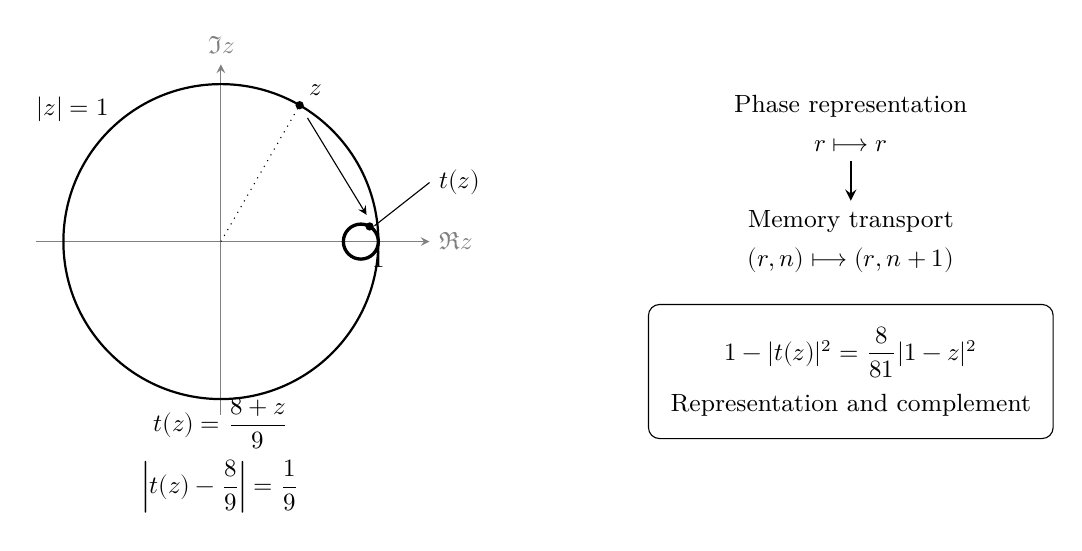
\begin{tikzpicture}[font=\small,>=stealth]
\begin{scope}[x=1cm,y=1cm]
\draw[->,gray] (-2.35,0)--(2.65,0) node[right] {$\Re z$};
\draw[->,gray] (0,-2.2)--(0,2.25) node[above] {$\Im z$};
\draw[thick] (0,0) circle (2);
\draw[very thick] (1.777778,0) circle (.222222);
\fill (1,1.732051) circle (1.5pt) node[above right] {$z$};
\fill (1.888889,.19245) circle (1.5pt);
\draw[->] (1.10,1.57)--(1.85,.34);
\draw[dotted] (0,0)--(1,1.732051);
\draw (1.95,.20)--(2.65,.75) node[right] {$t(z)$};
\node[below] at (2,0) {$1$};
\node[above left] at (-1.30,1.4) {$|z|=1$};
\node[align=center] at (0,-2.72)
 {$t(z)=\dfrac{8+z}{9}$\\[3pt]
 $\left|t(z)-\dfrac89\right|=\dfrac19$};
\end{scope}
\begin{scope}[shift={(8,0)}]
\node[align=center] (f) at (0,1.5) {Phase representation\\[3pt] $r\longmapsto r$};
\node[align=center] (m) at (0,0) {Memory transport\\[3pt] $(r,n)\longmapsto(r,n+1)$};
\draw[->,thick] (f)--(m);
\node[draw,rounded corners,inner sep=8pt,align=center] at (0,-1.65)
 {$1-|t(z)|^2=\dfrac8{81}|1-z|^2$\\[5pt]
 Representation and complement};
\end{scope}
\end{tikzpicture}
\caption{The circular chart of nonadic compression. On the left,
the unit circle and its image with center \(8/9\) and radius \(1/9\),
drawn to the same scale; the image of \(z=e^{i\pi/3}\) is shown.
On the right, phase return is accompanied by memory advancement.
The lower balance quantifies the complementary component. This figure
represents the map \(t\), distinct from the modal factor \(q=5/9\) of the
central chart.}
\label{fig:compresion-circular}
\end{figure}


The local Schur development gives the arithmetic form a positive sign on a concrete functional domain and its transport images. Identities \eqref{tm-add-balance-aritmetico}–\eqref{tm-add-balance-iterado} do not by themselves authorize declaring all their summands positive for an arbitrary test function: they locate exactly which energies and correlations an extension of that domain must preserve.


% SOURCE c L164-190
\subsection{Criterion for transporting positivity through mixed moments}
\label{tm-add-c5}
Let \(\mathcal D\) be the common domain of the previously constructed readouts. Let \(\mathscr W\) be the sesquilinear form expressed by their gamma, prime, and polar channels. The analytic formula is received after the native generator; it does not select the seeds or preceding coefficients.

Let \(C_a\) be the reversible transport on test functions and \(S\) the memory shift. We explicitly use \(C_a(\mathcal D)=\mathcal D\) and the identity \(\mathscr W(C_af,C_ag)=\mathscr W(f,g)\), proved for the exponential class of test functions in Subsections~\ref{tm-add-m4} and~\ref{tm-add-m5}. For a collection \(\mathcal E\subset\mathcal D\), suppose a linear map \(V:\operatorname{span}\mathcal E\to\mathcal K\) has been constructed such that, for every \(f,g\) in that collection and every integer \(n\),

\begin{equation}
\boxed{\mathscr W(C_a^n f,g)=\langle S^nVf,Vg\rangle.}
\label{tm-add-criterio-momentos}
\end{equation}
\begin{proposition}[Transport of positivity by identification of moments]
\label{tm-add-proposicion-costura-3}
Identity \eqref{tm-add-criterio-momentos} implies positivity of \(\mathscr W\) on the span of the orbits \(C_a^n\mathcal E\). If that space is dense in \(\mathcal D\) for the joint norm of the readouts, and these are continuous for that norm, positivity extends to \(\mathcal D\).
\end{proposition}

\begin{proof}
For \(F=\sum_j C_a^{n_j}f_j\), invariance of \(\mathscr W\) under \(C_a\) and \eqref{tm-add-criterio-momentos} give

\[
\begin{aligned}
\mathscr W(F,F)
&=\sum_{i,j}\mathscr W(C_a^{n_i-n_j}f_i,f_j)\\
&=\left\|\sum_i S^{n_i}Vf_i\right\|^2\geq0.
\end{aligned}
\]
If a combination represents the zero function, the same identity forces the vector combination to have zero norm; the realization is well-defined. Passage to the closure uses continuity of both readouts, not a subsequent choice of sign.
\end{proof}

This is a construction criterion with explicit domains, not an assertion that \eqref{tm-add-criterio-momentos} has been proved for all readouts of the corpus. Extension from the initial collection to its orbits requires preserving all cross moments: proving it only for \(n=0\) on that initial collection does not complete the extension. Naturally, a Gram identity already proved for \(n=0\) on all of \(\mathcal D\) would directly prove positivity on that domain.


% SOURCE c L191-211
\subsection{Energy identification and two-column realization}
\label{tm-add-c6}
The corpus preserves two columns \(J_+\) and \(J_-\) and an effective analytic connector between them. It also describes a native encoding \(\Xi\) and an orthogonal projection \(P\). When the two moment identities are calculated on the same domain,

\[
\langle\Xi f,\Xi g\rangle=\langle J_+f,J_+g\rangle,
\qquad
\langle P\Xi f,P\Xi g\rangle=\langle J_-f,J_-g\rangle,
\]
subtraction gives

\begin{equation}
\mathscr W(f,g)=\langle(I-P)\Xi f,(I-P)\Xi g\rangle.
\label{tm-add-dos-columnas}
\end{equation}
The dossier calculates the uniform expectation and Helmert refinement separately. Their joint conjugation preserves both Grams and cannot, by a mere change of notation, turn a difference operator into an evaluation operator. The recovered gamma connector realizes an additional analytic operation, which must preserve its energy budget. This clarification brings together existing operations; it does not declare the TPK architecture nonexistent.

Formulas \eqref{tm-add-criterio-momentos} and \eqref{tm-add-dos-columnas} are two compatible expressions of the route to be completed: the first organizes returns and their correlations; the second organizes the visible part and complementary memory. The Schur-complement estimate in the dossier gives effective control of that energy in a complete window and all its refinements. Its scope is stated with the concrete window, without replacing the global domain by that window.


% BEGIN PROCEDENCIA COSTURA, FUENTE L212
% ## 7. Localizadores materiales y continuidad
% 
% - APP central, modos \(9/5\): `base_c01_sin_encabezado.tex`, construcción de la carta central; capítulo `78_doble_circulo_campo_espectral_completo.tex`, entorno de líneas 1276–1280.
% - Memoria anterior a la representación espectral: `cap08_holonomia_helice_memoria.tex`, especialmente la cubierta entera y la publicación \(C_{108}\).
% - Conexión y compresión–expresión: `certificados/ley_nueve_puertas_2026-07-30/DELTA_CONEXION_NONADICA_CONJUNTA_COMPRESION_EXPRESION_2026-08-16.md`, §§1–3.
% - Doble círculo y transporte cilíndrico: propietario `78_doble_circulo_campo_espectral_completo.tex`, líneas 940–1260.
% - Dos momentos nativos: propietario `10b_prueba_espectral_polar_riemann_weil_rectificacion_probatoria_20260903.tex`, líneas 235–452.
% - Propietarios completos y rutas absolutas: [recuperación conservada](../ARITMETICA_GENEALOGICA_PRIMOS_DESARROLLO_DOBLE_CIRCULO_20260911/01_HALLAZGOS_PROPIETARIOS_DOBLE_CIRCULO.md).
% 
% La selección editorial sigue siendo el integral de 2.249 páginas y sus desarrollos adyacentes. Los verificadores históricos que devuelven 2.084 páginas no cambian esa selección. Ningún control de huellas o de compilación se utiliza aquí como prueba de positividad global.
% END PROCEDENCIA COSTURA

% SOURCE m L9-53
\subsection{Operator provenance and the function of the readouts}
\label{tm-add-m1}

% BEGIN LOCALIZADORES M1
% Propietarios y localizadores de esta lectura:
% 
% - Integral autoral de 2.249 páginas, propietario
%   `output/REVISION_EDITORIAL_HMT_MD_20260905/01_FUENTES/INTEGRAL/tree/New project/output/ENSAMBLADO_CAUSAL_RESTAURADO_HMT_MD_20260905/fuente/manuscrito/integracion_83/parte_v/tex/fuentes_propietarias/editor_ready/78_doble_circulo_campo_espectral_completo.tex`.
%   Se ha releído su cuerpo completo, 1–1929, en la copia conservada en el
%   manuscrito de primos. El cociclo está en 943–968; el orden
%   positividad → GNS → Stone → Cayley, en 525–612 y 969–987; el transporte
%   cilíndrico torcido, en 1023–1118; la pérdida por vuelta, en 1171–1237;
%   la costura de nueve fases, en 1421–1495; la fórmula aritmética, en 1578–1610.
% - `output/ARITMETICA_GENEALOGICA_PRIMOS_DESARROLLO_DOBLE_CIRCULO_20260911/01_HALLAZGOS_PROPIETARIOS_DOBLE_CIRCULO.md`, leído completo. Conserva los
%   localizadores de los antecedentes del bloque APP y de la memoria anteriores
%   al GNS; no se confunde su lectura con una nueva lectura íntegra de cada
%   antecedente que cita.
% - `output/ARITMETICA_GENEALOGICA_PRIMOS_PRESENTACION_20260911/antecedentes/recuperacion_gamma/narrativa_205_paginas/CONSTANTES_ESTRUCTURA_Y_REALIDAD_FISICA_RECOPILACION_INTEGRA.md`, lectura focal 5710–5905. En 5740–5869 reúne producto nativo,
%   irreducibles, ocupaciones, calor/Mellin, canal polar y los dos círculos.
%   No ofrece allí una secuencia Toeplitz adicional anterior a GNS.
% - `output/ARITMETICA_GENEALOGICA_PRIMOS_PRESENTACION_20260911/manuscrito/03_DOBLE_CIRCULO_Y_TRANSPORTE_ESPECTRAL.md`, §§2–3, para la forma completa,
%   su continuidad y las dos columnas; en este corte se ha releído §2,
%   líneas 119–191, y se conserva el análisis anterior de §3.
% - `output/AUDITORIA_INTEGRAL_PUBLICABILIDAD_HMT_MD_20260906/COORDINACION_20260906/TRAZA_GENERATIVA_COORDINADA.md`: consulta focal de lectores espectrales;
%   desde 1524 remite a los momentos primos, no a una medida circular de Weil
%   ya seleccionada por la memoria.
% 
% La puerta del núcleo permanente y su autocomprobación causal pasaron. La
% puerta histórica `apply-hmt-first-principles` resuelve 2.084 páginas; se conserva
% como control de ese testigo, no como sustituto de la selección autoral de
% 2.249 páginas. No se afirma lectura íntegra del corpus ni del documento de 205
% páginas.
% 
% END LOCALIZADORES M1
The chain used is APP → TRIT → TPK → enriched histories of the joint continuum → arithmetic and memory readouts → circular representation. The five continuum operations remain on the same histories; this development studies a readout of their memory and does not construct an isolated fifth branch. The prime readout uses irreducibles produced by the native product; constants already expressed by HMT enter the readouts only subsequently.

\textbf{Provenance.} Cocycle, loss, two sheets, memory groups, and double circle: preexisting authorial architecture and recovered results. The assembled proofs below are a new formalization of these antecedents. No historical priority is claimed for Poisson kernels, Cayley, or Toeplitz identities. The provenance of this exact composition within the corpus has not been exhaustively investigated beyond the source owners indicated.


% SOURCE m L54-83
\subsection{Regular memory representation preceding arithmetic GNS}
\label{tm-add-m2}
The central APP block, with its symmetric and antisymmetric projectors, is

\[
B_c=\begin{pmatrix}7&2\\2&7\end{pmatrix}
=9P_++5P_-.
\]
Normalization of the differential mode expresses \(q=5/9\). A complete TPK winding preserves phase and increments integer memory:

\[
m(\Gamma_9^n)=n,\qquad
m(\gamma_2\gamma_1)=m(\gamma_2)+m(\gamma_1).
\]
On a reversible orbit of that memory, its lifted states are identified with \(e_n\), \(n\in\mathbb Z\), and the winding is the shift \(Se_n=e_{n+1}\). Injectivity of this enumeration follows from the memory increment. If one starts only from the semigroup of positive windings, the same bilateral space is the shift extension adding its predecessors; reversibility is not attributed to a transition proved only isometric. In a complete tree, the remaining labels are preserved in a transverse factor: the shift acts on memory and does not identify routes.

This \(S\) is not the Weil Cayley operator inserted into the seam. It is the regular realization of the integer memory operation. Its Hilbert-space positivity is known before forming a GNS of the arithmetic form.


% SOURCE m L84-120
\subsubsection{Loss vector, correlations, and terminal term}
\label{tm-add-m2-1}
Telescoping over windings produces weights \((1-q^2)q^{2j}\). Their amplitude in memory is the explicit vector

\[
v_q=\sqrt{1-q^2}\sum_{j=0}^{\infty}q^j e_j,
\qquad \|v_q\|^2=1.
\]
With inner product linear in the first variable, for \(n\ge0\),

\[
\langle S^n v_q,v_q\rangle
=(1-q^2)\sum_{j\ge0}q^j q^{j+n}=q^n.
\]
Conjugation and unitarity give, for every integer,

\[
\boxed{m_n^{\mathrm{mem}}=q^{|n|}.}
\]
The truncation \(v_{q,N}=\sqrt{1-q^2}\sum_{j=0}^{N-1}q^j e_j\) preserves the terminal exactly:

\[
\|v_{q,N}\|^2=1-q^{2N},\qquad
\langle S^n v_{q,N},v_{q,N}\rangle
=q^n\bigl(1-q^{2(N-n)}\bigr),\quad 0\le n<N.
\]
For \(n\ge N\), that truncated correlation is zero. Thus, for each fixed \(n\), the difference from the complete moment is \(q^{2N-n}\) when \(N>n\), and tends to zero. This formula neither erases the last register nor equates a truncation with the whole history.


% SOURCE m L121-159
\subsubsection{Triangular factorization and determinant of the memory matrices}
\label{tm-add-m2-2}
For indices \(0,\ldots,N\), define

\[
T_N=(q^{|i-j|})_{0\le i,j\le N}.
\]
It is a Gram matrix of \(v_q,Sv_q,\ldots,S^Nv_q\), so

\[
\sum_{i,j=0}^{N}\overline{c_i}c_j(T_N)_{ij}
=\left\|\sum_{j=0}^{N}c_jS^jv_q\right\|^2\ge0.
\]
There is also an exact proof without infinite series. Let

\[
L_{ij}=\begin{cases}q^{i-j},&i\ge j,\\0,&i<j,\end{cases}
\qquad D=\operatorname{diag}(1,1-q^2,\ldots,1-q^2).
\]
Then \(T_N=LDL^*\). For \(i\ge j\), the product entry is

\[
q^{i+j}+(1-q^2)\sum_{k=1}^{j}q^{i+j-2k}
=q^{i-j}.
\]
Symmetry gives the full matrix identity. A Cholesky factor is \(L D^{1/2}\), and, since \(\det L=1\),

\[
\boxed{\det T_N=(1-q^2)^N=(56/81)^N>0.}
\]
This positive kernel arises from loss and preserved memory. It requires no zeros, positive zeta function, or Weil GNS.


% SOURCE m L160-184
\subsection{Phase, nonadic refinement, and weak convergence of states}
\label{tm-add-m3}
A fixed-phase representation is obtained from

\[
v_{r,\theta}=\sqrt{1-r^2}\sum_{j\ge0}r^j e^{-ij\theta}e_j,
\quad 0<r<1,
\]
and produces \(m_n=r^{|n|}e^{in\theta}\). The Toeplitz matrices are diagonal conjugates of the preceding ones and have determinant \((1-r^2)^N\). Here the phase \(\theta\) is a coordinate of the character collection; no arithmetic spectral phase has been selected.

On the circle, with normalized Haar measure \(d\lambda\), these moments have the explicit measure

\[
d\nu_{r,\theta}(z)
=\frac{1-r^2}{|1-r e^{-i\theta}z|^2}\,d\lambda(z).
\]
Expanding both geometric series directly proves its Fourier coefficients without using a target measure.


% SOURCE m L185-219
\subsubsection{Nonadic roots of the radius and phase compatibility}
\label{tm-add-m3-1}
Taking \(r_m=q^{1/9^m}\), one has \(0<r_m<1\), \(r_{m+1}^{9}=r_m\), and \(r_m\to1\). For fixed phase,

\[
r_m^{|n|}e^{in\theta}\longrightarrow e^{in\theta}
\quad\text{for each }n\in\mathbb Z.
\]
The measures are probabilities; uniform approximation by trigonometric polynomials extends moment convergence to every continuous function. Consequently,

\[
\nu_{r_m,\theta}\ \rightharpoonup\ \delta_{e^{i\theta}}.
\]
This shows how an atomic measure can arise as a weak limit of memory states. It is not a strong limit of the vectors in the same regular representation: each coefficient of \(v_{r_m,\theta}\) tends to zero, but their norms remain one.

A naturality qualification must be preserved. Under \(p_9(z)=z^9\),

\[
(p_9)_*\nu_{r,\theta}=\nu_{r^9,9\theta}.
\]
Thus the nonadic radius with fixed phase does \textbf{not} by itself give a projective system of measures under \(p_9\). This requires retaining lifted phases with \(9\theta_{m+1}=\theta_m\pmod{2\pi}\), including their branch choices; alternatively, one must declare that the refinement used keeps the angular coordinate fixed and changes only the radius. These are different operations.


% SOURCE m L220-236
\subsubsection{State selection and change of spectral type}
\label{tm-add-m3-2}
Memory produces the group, positivity of its Grams, and these compatible correlation collections. A particular phase or a mixture of phases requires the readout selecting its amplitudes. For example, the vector \(e_0\) produces \(m_n=\mathbf1_{n=0}\); \((e_0+e_1)/\sqrt2\) produces \(m_0=1,m_{\pm1}=1/2\), with all other moments zero. The same memory operation admits both positive states.

The regular representation has vector measures absolutely continuous with respect to Haar measure. A fixed \(L^2\) vector filter cannot produce a nonzero purely atomic measure. The preceding weak limit shows a precise way for spectral type to change under refinement: that limit of states must be preserved and controlled, rather than merely increasing the length of a previously chosen phase orbit. This does not deny the spectral representation of the corpus or joint HMT generation; it distinguishes the domains of two readouts.


% SOURCE m L237-295
\subsection{Cayley operator on the exponential test-function domain}
\label{tm-add-m4}
A second object is now constructed, without assuming Weil positivity. The native product and its irreducibles already provide \(\ell_{p,k}=k\log p\), \(w_{p,k}=(\log p)p^{-k/2}\). The gamma and polar readouts complete the form \(\mathscr W\) written in Subsection~\ref{tm-add-m5}. Memory supplies an integer iteration index; the following operator acts effectively on the functions of that representation.

The operator \(C_a\) is an auxiliary analytic readout of this formalization. The choice \(a>1/2\) does not silently replace the canonical seam \(a=1/2\), nor is it declared that this choice has already been selected by the TPK.

Fix \(a>b>1/2\). Let \(\mathscr E_b\) be the space of smooth functions such that, for each derivative order \(j\), \(\sup_x e^{b|x|}|f^{(j)}(x)|<\infty\). It contains all compactly supported test functions. Define

\[
(R_a^+f)(x)=\int_0^\infty e^{-at}f(x+t)\,dt,
\qquad
(R_a^-f)(x)=\int_0^\infty e^{-at}f(x-t)\,dt,
\]
\[
\boxed{C_af=f-2aR_a^+f,\qquad C_a^{-1}f=f-2aR_a^-f.}
\]
These integrals are translation readouts constructed on the test functions; they do not use the spectrum of zeros. The parameter \(a=1\), for example, comes from the unit and allows a choice \(1/2<b<1\); it calibrates no zero.

\paragraph{Domain, inverse, and unitary realization.} The inequality \(e^{b|x|}|f(x\pm t)|\le M_0e^{bt}\) gives the bound \(\|R_a^\pm f\|_b\le\|f\|_b/(a-b)\), also for every derivative. Thus both operators preserve \(\mathscr E_b\). With the convention \(\widehat f(z)=\int f(x)e^{-izx}\,dx\), their multipliers are

\[
\widehat{C_af}(z)=c_a(z)\widehat f(z),\qquad
c_a(z)=\frac{z-ia}{z+ia},
\]
and the inverse operator has multiplier \(c_a(z)^{-1}\). The identity on the real Fourier axis proves both inverse compositions. In \(L^2\), \(|c_a(t)|=1\), so \(C_a\) is unitary for the ordinary norm, without using the Weil norm. On test functions it can be written \(C_a=(H+ia)(H-ia)^{-1}\), with \(H=i\partial_x\); here the integral formula, not a GNS generator, defines the operators.

\paragraph{Convergence condition at the polar boundary.} The parameter \(a=1/2\) of the source owner's Cayley operator cannot simply be inserted into these pre-GNS integrals. For a compactly supported test function, \(R_{1/2}^+f\) generally has a tail proportional to \(e^{x/2}\) towards \(-\infty\); its negative polar evaluation does not converge. Divergence of the assembled form has not been proved; rather, this term-by-term decomposition requires the margin \(a>1/2\). The GNS Cayley operator may subsequently use \(a=1/2\) on its Hilbert-space domain.


% SOURCE m L296-352
\subsection{Joint preservation of the gamma, prime, and polar channels}
\label{tm-add-m5}
For \(f,g\in\mathscr E_b\), let

\[
C_{f,g}(u)=\int f(x)\overline{g(x-u)}\,dx,
\qquad P_f^\pm=\int f(x)e^{\pm x/2}\,dx.
\]
The complete form is defined by

\[
\begin{aligned}
\mathscr W(f,g)={}&c_\Gamma C_{f,g}(0)
+\int_0^\infty\frac{e^{-u/2}}{1-e^{-2u}}
 [2C_{f,g}(0)-C_{f,g}(u)-C_{f,g}(-u)]\,du\\
&-\sum_{p,k}w_{p,k}
 [C_{f,g}(\ell_{p,k})+C_{f,g}(-\ell_{p,k})]\\
&+P_f^+\overline{P_g^-}+P_f^-\overline{P_g^+},
\qquad c_\Gamma=\psi(1/4)-\log\pi.
\end{aligned}
\]
\paragraph{Existence and continuity of the complete form.} The correlation bound \(|C_{f,g}(u)|\le M_fM_g(|u|+1/b)e^{-b|u|}\) proves absolute convergence of the prime sum, dominated by a series of the form \(\sum_{n\ge2}(\log n)(1+\log n)n^{-b-1/2}\). The symmetric correlation difference is \(O(u^2)\) at zero, whereas the gamma weight is \(O(u^{-1})\); at infinity the weight is exponential. Polar evaluations converge because \(b>1/2\). These bounds also prove continuity in the indicated seminorms. Positivity is not used.

\paragraph{Simultaneous invariance of the three channels.}
\label{tm-add:invariancia-weil} Since \(C_a\) is unitary on \(L^2\) and commutes with all translations,

\[
C_{C_af,C_ag}(u)=C_{f,g}(u)\qquad(u\in\mathbb R).
\]
By Fubini, the two polar readouts satisfy

\[
P_{C_af}^+=-\frac{a-1/2}{a+1/2}P_f^+,
\qquad
P_{C_af}^-=-\frac{a+1/2}{a-1/2}P_f^-.
\]
The factors are real and reciprocal, so each cross polar product is preserved exactly. Combining the three channels,

\[
\boxed{\mathscr W(C_af,C_ag)=\mathscr W(f,g).}
\]
The identity holds for all integer powers and all cross terms. It proves invariance of a Hermitian form, not its sign.


% SOURCE m L353-383
\subsection{Circular moments of the complete arithmetic form}
\label{tm-add-m6}
Define

\[
m_n^{\mathrm{ar}}(f,g)=\mathscr W(C_a^n f,g),\qquad n\in\mathbb Z.
\]
The complete formula in Subsection~\ref{tm-add-m5}, with \(C_a^nf\) in its first argument, calculates these moments from primes, gamma, and polar terms. Each evaluation exists in \(\mathscr E_b\); it requires neither a list of zeros nor a positive metric. Hermiticity and the preceding invariance give

\[
m_{-n}^{\mathrm{ar}}(g,f)=\overline{m_n^{\mathrm{ar}}(f,g)},\qquad
\mathscr W(C_a^j f,C_a^k g)=m_{j-k}^{\mathrm{ar}}(f,g).
\]
For a single test function, the matrix \(T_N^{\mathrm{ar}}(f)_{jk}=m_{k-j}^{\mathrm{ar}}(f,f)\) is Hermitian Toeplitz and satisfies the exact identity

\[
c^*T_N^{\mathrm{ar}}(f)c
=\mathscr W\!\left(\sum_{k=0}^N c_k C_a^k f,
                    \sum_{k=0}^N c_k C_a^k f\right).
\]
The matrix has been constructed without assuming positivity. The equality allows its positivity to be compared with a native memory Gram; it does not presuppose it.


% SOURCE m L384-406
\subsubsection{Polar growth and a necessary cancellation condition}
\label{tm-add-m6-1}
For \(a=1\), the exact polar contribution to \(m_n^{\mathrm{ar}}(f,g)\) is

\[
(-1/3)^nP_f^+\overline{P_g^-}
+(-3)^nP_f^-\overline{P_g^+}.
\]
For a nonzero real, even, positive test function, \(P_f^+=P_f^-=p>0\), so \(p^2[(-1/3)^n+(-3)^n]\) appears. If the total moment sequence is positive definite, its order-two minors force

\[
|m_n^{\mathrm{ar}}(f,f)|\le m_0^{\mathrm{ar}}(f,f).
\]
Thus circular identification must account for the concrete cancellation of this growth with the gamma and prime channels. Formal symmetry of the two sheets does not replace that calculation. This observation does not declare that cancellation fails; it provides an exact falsifier for a candidate composition.


% SOURCE m L407-424
\subsubsection{Mixed moment matrices and domain coverage}
\label{tm-add-m6-2}
For a collection of test functions \(f_1,\ldots,f_d\), the appropriate object is the block Toeplitz matrix

\[
\mathsf T_{(j,r),(k,s)}
=m_{k-j}^{\mathrm{ar}}(f_s,f_r).
\]
Its quadratic form is \(\mathscr W(F,F)\), where \(F=\sum_{k,s}c_{k,s}C_a^k f_s\). Controlling only the scalar matrices of some test functions does not control cross terms between different test functions. For a dense collection in each \(C_c^\infty([-R,R])\), the continuity proved above permits passage to the complete domain, provided the mixed Grams and compatibilities as \(R\) increases have been established. Increasing \(N\) along a single orbit does not prove that coverage.


% SOURCE m L425-477
\subsubsection{Transport of local coercivity to subspaces with tails}
\label{tm-add-m6-3}
\label{tm-add:familias-transportadas}
The preceding identity has a positive application that does not yet require identifying all moments with memory. Suppose the Schur complement has proved, on the interval \(I=(-1/18,1/18)\), the bound

\[
\mathscr W(f,f)\geq\tfrac12\|f\|_{L^2}^2,
\qquad f\in C_c^\infty(I).
\]
This subsection receives that estimate as a result of the corresponding local calculation; it does not deduce it from the existence of \(C_a\). Let \((\tau_t f)(x)=f(x-t)\). Translation preserves correlations and satisfies

\[
P_{\tau_t f}^{\pm}=e^{\pm t/2}P_f^{\pm}.
\]
Its cross polar products are also preserved. Therefore \(\mathscr W(\tau_t f,\tau_t g)=\mathscr W(f,g)\), and the ordinary \(L^2\) norm is invariant. Since \(C_a\) and \(\tau_t\) commute, for every integer \(n\), every \(t\in\mathbb R\), and every local test function,

\[
\boxed{\mathscr W(C_a^n\tau_t f,C_a^n\tau_t f)
=\mathscr W(f,f)
\geq\tfrac12\|C_a^n\tau_t f\|_{L^2}^2.}
\]
For fixed \((n,t)\), this is a coercive bound on the entire subspace \(C_a^n\tau_t C_c^\infty(I)\), not merely on one example. When \(n\ne0\), transformed test functions may have noncompact exponential tails. Infinitely many prime clocks may enter their arithmetic form; exact equality of the three channels controls their composition, and the bounds in Subsection~\ref{tm-add-m5} guarantee convergence. That sum has not been replaced by a finite truncation.

Cross terms between subspaces with different exponents or translations, by contrast, retain their complete moments. For example,

\[
\mathscr W(C_a^n\tau_t f,C_a^m\tau_s g)
=\mathscr W(C_a^{n-m}\tau_{t-s}f,g).
\]
The bound on each individual subspace does not imply positivity of their algebraic sum. This is decided through the mixed Grams in Subsection~\ref{tm-add-m6-2}. An effective positive scope—entire collections of test functions with tails—is thus isolated without promoting it to the whole domain solely through transport invariance.


% SOURCE m L478-521
\subsection{Prospective identification of moments and energy}
\label{tm-add-m7}
Memory already produces the positive regular representation of
Subsection~\ref{tm-add-m2}; the arithmetic channels produce \(C_a\)
and \(m_n^{\mathrm{ar}}\) without GNS. Formulating the global step also requires
specifying the representation that receives the state limit.
Denote that space by \(\mathcal K_{\rm lim}\) and its unitary winding
operator by \(U_{\rm mem}\), both to be constructed
from histories and limit compatibilities. They are not
identified in advance with the regular space and its shift \(S\).
A prospective identification has the form

\[
\boxed{m_n^{\mathrm{ar}}(f,g)
=\langle U_{\rm mem}^{\,n}\mathcal E f,\mathcal E g\rangle_{\mathcal K_{\rm lim}}}
\]
for a readout \(\mathcal E\) constructed from operations on the same histories and not defined as \(\mathscr W^{1/2}\). In that case, all mixed Toeplitz matrices are Grams; arithmetic GNS follows as a realization of a product already obtained.

It suffices to prove the zeroth-moment identity and the intertwining
\(\mathcal E C_a=U_{\rm mem}\mathcal E\), with the stated domains and
compatibilities. The zeroth moment is identification of the
complete energy, not a lesser condition: it cannot be regarded as proved
merely because an \(\mathcal E\) with some positive Gram exists.

\paragraph{Why distinguishing the representations matters.}
The regular shift on \(\ell^2(\mathbb Z;\mathcal K)\)
has no nonzero eigenvectors. Since \(S\) is unitary, any
eigenvalue would have modulus \(1\). Indeed, if \(Sx=\lambda x\)
with \(|\lambda|=1\), the coordinate relation forces
\(\|x_n\|\) to be constant; square summability forces \(x=0\).
Thus a representation with a nonzero eigenvector admits
no isometric intertwiner into that shift: the image would be
a nonzero eigenvector of \(S\). This observation applies to
atomic arithmetic GNS if its global hypotheses hold. It does not
contradict weak convergence of states in
Subsection~\ref{tm-add-m3-2}; it shows that the limit requires its own
representation and not a limit vector in the original regular space.
Construction of \((\mathcal K_{\rm lim},U_{\rm mem})\) and the
readout identifying the moments is part of the prospective condition,
not a consequence already proved from the regular Grams.

In the manuscript's two-column form, the calculation remains

\[
\Xi^*\Xi=J_+^*J_+,\qquad
\Xi^*P\Xi=J_-^*J_-,\qquad
\mathcal E=(I-P)\Xi.
\]
If \(P\) is an orthogonal projection, these two equalities produce \(\mathcal E^*\mathcal E=J_+^*J_+-J_-^*J_-\). Verifying only one of them does not suffice, nor does replacing the complete columns with those of an isolated gamma block. The phases and moments in this development make explicit what that composition must transmit to all windings.

The kernel \(q^{|n|}\) is not identified here with \(m_n^{\mathrm{ar}}(f,g)\). It is an effective positive antecedent and offers a local factorization; the readout \(\mathcal E\) must also preserve prime labels, weights, polar contributions, and the state limit if spectral type changes. Declaring that equality by definition would introduce the result one seeks to construct.


% SOURCE m L522-544
\subsection{Exact checks and scope of the composition}
\label{tm-add-m8}

% BEGIN CONTROL DOCUMENTAL M8
% El archivo `verificar_momentos_memoria.py` conserva 1.046 comprobaciones exactas con
% fracciones racionales: factorización \(LDL^*\) y determinantes en dimensiones
% 1–13 para \(q=5/9\), correlaciones truncadas hasta 20 posiciones y factores
% polares recíprocos para cuatro valores racionales de \(a>1/2\). Se ejecuta
% con `/usr/bin/python3 -I -S` y admite también `-O`; sus condiciones no
% dependen de instrucciones `assert`. Los recibos focales son
% `CONTROL_MOMENTOS_MEMORIA_NORMAL.json` y
% `CONTROL_MOMENTOS_MEMORIA_OPTIMIZADO.json`. No se ejecutó aquí una campaña intervalar de momentos
% de Weil, ni se convierten esos controles en una prueba global.
% 
% END CONTROL DOCUMENTAL M8
The executable verification preserves 1,046 exact checks with rational fractions: \(LDL^*\) factorization and determinants in dimensions 1–13 for \(q=5/9\), truncated correlations through 20 positions, and reciprocal polar factors for four rational values of \(a>1/2\). Ordinary and optimized executions use explicit conditions independent of assertion instructions. Their sources, commands, and receipts are preserved in the reproduction dossier. No interval campaign of Weil moments was run here, nor are these checks converted into a global proof.

The usable advance is twofold: loss memory produces a positive Toeplitz kernel with explicit Cholesky factor and terminal, and the complete form admits an integral Cayley operator preceding GNS that constructs its circular moments and preserves each channel. Nonadic regularization also shows how to pass from regular states to atoms by a weak limit, with its phase condition correctly separated. The union of both constructions retains identification of the two complete moments as a precise equation.

This development neither refutes that union, proves its absence throughout the corpus, nor declares it established by the local identities. It leaves a concrete composition that can be compared and developed in the continuation of this manuscript.

\clearpage
\clearpage
\section[Boundary expectations and reconstruction of the analytic channels]{Boundary expectations and\\reconstruction of the analytic channels}
\label{sec:lectores-gamma}
% Fuente íntegra: ampliacion/expediente/AGENTE_CARTAS_Y_EXPECTATIVA.md

% PROCEDENCIA Fecha del corte: 11 de septiembre de 2026. Nota interna de desarrollo, no modificación de un artículo ni dictamen global sobre HMT. No se ha comunicado a otras tareas del usuario.

\subsection{Action of the readouts and content of the moments}
\label{gamma-add-sub-5}

The explicit actions of the odometer, the difference readout, the uniform inclusion, the Helmert refinement, the bidirectional boundary, and the polar chart have been recovered and composed. The calculation yields:

\begin{enumerate}
\item The moments of the positive and negative columns, considered separately, are determined by explicit operators. They include all cross products between test functions.
\item The uniform expectation does not coincide with the Helmert refinement. On the carry mode it yields an exact factor, calculated below; it does not by itself convert a translation difference into the uniform mode.
\item The gamma-tail resolvent does perform the analytic conversion and exactly reconstructs all negative rows, on every window and before any sign is used.
\item The simultaneous identification of the first moment of the encoder and the moment of its projection does not follow from the three preceding chart identities by a simple direct sum. The specific additional composition that must be verified is identified below. The structural readout is not declared absent, nor is this focal check identified with the full TPK.

\end{enumerate}
The advance consists in calculating the action and cross products, not in reiterating that the projection is positive.

\paragraph{Provenance of the charts.}
The formulas are assembled from the developments \emph{Polar spectral proof},
\emph{Form and Gram}, \emph{Gamma-tail connector}, \emph{Odometer and
carry}, \emph{Pulsation and expectation}, and \emph{Modular polar chart}.
The locators and the record of the reading performed are retained in the
source dossier accompanying the delivery. Each chart is used with the spaces,
normalizations, and identities made explicit below; a
documentary reference does not replace these conditions.

% DOCUMENTACION ## 2. Propietarios y lectura efectuada
% DOCUMENTACION 
% DOCUMENTACION Se utilizan estos propietarios, leídos completos en esta formalización:
% DOCUMENTACION 
% DOCUMENTACION - **P10**: [10b — prueba espectral polar](</Users/ruben/Documents/New project/output/ARTICULO_VIII_PRIMOS_ESTRUCTURA_ESPECTRAL_20260910/antecedentes/integral/manuscrito/sucesor_102/deltas_ley9/10b_prueba_espectral_polar_riemann_weil_rectificacion_probatoria_20260903.tex>), 1.166 líneas. Las columnas están en 151–235; la expectativa y el codificador nativo en 288–367; la transferencia derivada de los momentos en 369–452; el codificador escrito mediante el complemento, más adelante, utiliza la identidad energética ya obtenida.
% DOCUMENTACION - **PG**: [Forma y Gram](</Users/ruben/Documents/excelencia academica/ARTICULOS_CIENTIFICOS_HMT_MD_2026-08-14/RIEMANN_REDHEFFER_WEIL/manuscrito/secciones/00_forma_y_gram.tex>), 630 líneas. Fórmulas explícitas de los dos modos y del refinamiento: 133–191; columnas: 194–220; codificador y momentos comunes: 222–304.
% DOCUMENTACION - **PT**: [Conector de cola gamma](</Users/ruben/Documents/excelencia academica/ARTICULOS_CIENTIFICOS_HMT_MD_2026-08-14/RIEMANN_REDHEFFER_WEIL/manuscrito/secciones/02b_conector_cola_gamma.tex>), completo. Inversión: 1–45; elevación y frontera: 47–155; todas las filas negativas: 157–242; restricción alcanzable: 250–269.
% DOCUMENTACION - **PO**: [Odómetro y acarreo](</Users/ruben/Documents/excelencia academica/CLAUSURA_WEIL_HMT_PULSACION_NONADICA_2026-08-11/PUBLICACION_WEIL_RIEMANN_HMT_MD_REVISION_EDITORIAL_2026-08-12/manuscrito/sections/03_odometro_carry.tex>), completo.
% DOCUMENTACION - **PE**: [Pulsación y expectativa](</Users/ruben/Documents/excelencia academica/CLAUSURA_WEIL_HMT_PULSACION_NONADICA_2026-08-11/PUBLICACION_WEIL_RIEMANN_HMT_MD_REVISION_EDITORIAL_2026-08-12/manuscrito/sections/02_pulsacion_y_expectativa.tex>), completo.
% DOCUMENTACION - **PP**: [Carta polar modular](</Users/ruben/Documents/excelencia academica/CLAUSURA_WEIL_HMT_PULSACION_NONADICA_2026-08-11/PUBLICACION_WEIL_RIEMANN_HMT_MD_REVISION_EDITORIAL_2026-08-12/manuscrito/sections/06_canal_polar_modular.tex>), completo. Carta Witt–dodecafase: 134–181.
% DOCUMENTACION - [Acarreo ortogonal del residual](</Users/ruben/Documents/excelencia academica/ARTICULOS_CIENTIFICOS_HMT_MD_2026-08-14/RIEMANN_REDHEFFER_WEIL/manuscrito/secciones/00d_carry_ortogonal_app_weil.tex>), completo.
% DOCUMENTACION 
% DOCUMENTACION Se contrastó además el propietario de las cinco realizaciones del continuo del 17 de agosto, sección de Riemann desde su objeto hasta el transporte del complemento, sin disgregar esas construcciones: allí se vuelve a formular el mismo par de momentos nativos. La consulta de esa sección no equivale a una lectura íntegra de todo ese manuscrito.
% DOCUMENTACION 
% DOCUMENTACION Los antecedentes de agosto se consultan como propietarios de las fórmulas que P10 reutiliza, no como sustitutos de la selección autoral del integral de 2.249 páginas. Los localizadores globales que todavía resuelven 2.084 páginas quedan registrados como históricos para esta serie.
% DOCUMENTACION 
\subsection{Conventions and genealogical cutoff}
\label{gamma-add-sub-32}

The relevant starting point is the APP--TRIT--TPK state, its refinement with memory, and its native readouts. In this formalization:

\begin{itemize}
\item APP provides the support and the irreducible selector. The native product, coproductivity, and selector precede the representation of prime--power labels.
\item TRIT and sheet transport preserve orientation and the seam.
\item The TPK preserves the phase step and the carry register; its odometer induces the translation difference. The logarithmic representation of the clocks produces \(\ell_{p,k}=k\log p\) and \(w_{p,k}=(\log p)p^{-k/2}\).
\item The boundary and polar charts are subsequent realizations of the same readouts. No state is selected by means of zeta zeros or a target value.

\end{itemize}
This section calculates the arrow between these readouts and the expectation, after their common generation; it does not seek to reconstruct or replace the joint continuum.

We work with orthonormal history coordinates. In these coordinates, \(u_N=N^{-1/2}(1,\ldots,1)\). If functions with the uniform probability measure are used, the constant coordinates and averages are conjugated by the corresponding normalization factor; the projections and all the norm ratios below remain the same.

Let \(H=L^2(\mathbb R)\), \(T_af(x)=f(x-a)\), \(\mathcal D_R=C_c^\infty((-R/2,R/2))\). We write \(d_a=T_a-I\); changing simultaneously to \(I-T_a\) preserves their Grams but changes the sign of the inverting cotrace.

The inner product is linear in the first variable. We retain the
polar evaluations and the scalar of the full form,
\begin{equation}
\begin{aligned}
A_f&=\int_{\mathbb R}f(x)e^{x/2}\,dx,
&B_f&=\int_{\mathbb R}f(x)e^{-x/2}\,dx,\\
c_\Gamma&=-\gamma-\frac\pi2-3\log2-\log\pi<0,
&\mu(a)&=\frac{e^{-a/2}}{1-e^{-2a}}.
\end{aligned}
\label{gamma-add-def-evaluaciones}
\end{equation}
Here \(\pi\), \(\gamma\), and the logarithms retain the internal
representation and subsequent realization declared in the preceding chapters.
The formula introduces no target values into the generator.

\subsection{Action of the odometer on generators}
\label{gamma-add-sub-47}

For \(N=9^m\), \(m\ge1\), with the seam located at the first vector,

\begin{equation}
U_{a,N}(e_r\otimes f)=
\begin{cases}
e_{r+1}\otimes f,&r<N-1,\\
e_0\otimes T_af,&r=N-1.
\end{cases}
\label{gamma-add-display-1}
\end{equation}

The uniformization \(i_Nf=u_N\otimes f\) gives

\begin{equation}
U_{a,N}i_Nf
=u_N\otimes f+N^{-1/2}e_0\otimes d_af.
\label{gamma-add-display-2}
\end{equation}

Therefore, for \(P_N=|u_N\rangle\langle u_N|\otimes I\),

\begin{equation}
\begin{aligned}
i_N^*U_{a,N}i_N&=I+\frac{d_a}{N},\\
(I-P_N)U_{a,N}i_N
&=\frac{\sqrt{N-1}}{N}\eta_N\otimes d_a.
\end{aligned}
\label{gamma-add-display-3}
\end{equation}

where

\begin{equation}
\eta_N=\frac{Ne_0-\mathbf1_N}{\sqrt{N(N-1)}}.
\label{gamma-add-display-4}
\end{equation}

This recovers the normalized difference readout:

\begin{equation}
\widehat\delta_{a,m}f=\eta_N\otimes u_{81}\otimes d_af,
\qquad
j_mf=u_N\otimes u_{81}\otimes f.
\label{gamma-add-display-5}
\end{equation}

The action on any combination of generators, without removing their cross terms, is

\begin{equation}
\left\langle\sum_i\widehat\delta_{a_i,m}f_i,
                  \sum_j\widehat\delta_{b_j,m}g_j\right\rangle
=\sum_{i,j}\langle d_{a_i}f_i,d_{b_j}g_j\rangle.
\label{gamma-add-display-6}
\end{equation}

In particular,

\begin{equation}
\widehat\delta_{a,m}^*\widehat\delta_{b,m}=d_a^*d_b,\qquad
j_m^*j_m=I,\qquad
j_m^*\widehat\delta_{a,m}=0.
\label{gamma-add-eq-1}
\end{equation}

The last cross product follows from \(\langle u_N,\eta_N\rangle=0\). It is concrete information about the orientation of the modes, in addition to the two isolated norms.

\subsection{Two distinct refinements and their expectations}
\label{gamma-add-sub-108}

\subsubsection{Uniform inclusion and projection of the last digit}
\label{gamma-add-sub-110}

Write \(M=9N\) and \(\mathbb C^M=\mathbb C^N\otimes\mathbb C^9\). The inclusion and its adjoint are

\begin{equation}
\iota_Nx=x\otimes u_9,\qquad
E_N=I_N\otimes\langle u_9|,\qquad P_N^{\rm unif}=\iota_NE_N.
\label{gamma-add-display-8}
\end{equation}

Acting in coordinates,

\begin{equation}
E_Nu_M=u_N,\qquad
E_N\eta_M=a_N\eta_N,\qquad
a_N=\sqrt{\frac{N-1}{9N-1}}.
\label{gamma-add-eq-2}
\end{equation}

\begin{proof}
We have \(E_Ne_0^{(M)}=e_0^{(N)}/3\) and \(E_N\mathbf1_M=3\mathbf1_N\).
Substitution into \(\eta_M=(Me_0-\mathbf1_M)/\sqrt{M(M-1)}\)
yields \eqref{gamma-add-eq-2}.
\end{proof}

Consequently,

\begin{equation}
(E_N\otimes I)\widehat\delta_{a,m+1}=a_N\widehat\delta_{a,m},
\qquad
(E_N\otimes I)j_{m+1}=j_m.
\label{gamma-add-eq-3}
\end{equation}

All projected moments are determined:

\begin{equation}
\begin{aligned}
\widehat\delta_{a,m+1}^*(P_N^{\rm unif}\otimes I)\widehat\delta_{b,m+1}
 &=a_N^2d_a^*d_b,\\
j_{m+1}^*(P_N^{\rm unif}\otimes I)j_{m+1}&=I,\\
j_{m+1}^*(P_N^{\rm unif}\otimes I)\widehat\delta_{b,m+1}&=0.
\end{aligned}
\label{gamma-add-eq-4}
\end{equation}

The complementary fraction of the carry is \(1-a_N^2=8N/(9N-1)\). For \(N=9\), the expressed fraction is \(1/10\), not \(1\), and its output remains a difference.

We do not conflate \(P_N^{\rm unif}\), which averages the last digit, with the projection onto the single global line \(u_M\): the latter annihilates \(\eta_M\) entirely.

\subsubsection{Helmert refinement}
\label{gamma-add-sub-156}

The operator \(W_N\) is fixed by the orthonormal Helmert bases
of the two levels, ordered to preserve the uniform and
carry modes. It is the isometry that sends the first \(N\) vectors of the
basis at level \(N\) to the corresponding vectors of the basis at level \(M\).
In particular, it satisfies

\begin{equation}
W_Nu_N=u_M,\qquad W_N\eta_N=\eta_M,\qquad W_N^*W_N=I.
\label{gamma-add-display-12}
\end{equation}

Thus, \(E_N^{\rm H}=W_N^*\), \(P_N^{\rm H}=W_NW_N^*\) give

\begin{equation}
E_N^{\rm H}j_{m+1}=j_m,\qquad
E_N^{\rm H}\widehat\delta_{a,m+1}=\widehat\delta_{a,m}.
\label{gamma-add-eq-5}
\end{equation}

The uniform--carry cross product remains zero, and that of two differences remains \(d_a^*d_b\). The refinement is therefore natural for both modes, but does not transform one into the other. Specifically, \(W_N\ne\iota_N\).

\subsubsection{Conjugation of expectations and preservation of moments}
\label{gamma-add-sub-174}

There is a unitary \(S_M\) on \(\mathbb C^M\) that maps \(\iota_N\mathbb C^N\) to \(W_N\mathbb C^N\), with \(W_N=S_M\iota_N\). It suffices to map the two orthonormal bases to each other and complete the complements. Then

\begin{equation}
P_N^{\rm H}=S_MP_N^{\rm unif}S_M^*.
\label{gamma-add-display-14}
\end{equation}

Conjugating the state \(C\) and its projection simultaneously,

\begin{equation}
(S_MC)^*(S_MP S_M^*)(S_MC)=C^*PC,\qquad
(S_MC)^*(S_MC)=C^*C.
\label{gamma-add-eq-6}
\end{equation}

Neither moment changes. If only the projection is changed, the fraction in this case goes from \(a_N^2\) to \(1\), but the analytic operator remains \(d_a\), not \(I\).

More generally, for any projection acting only on the finite history fiber, the moment of a single channel is
\(\langle\eta,P\eta\rangle d_a^*d_b\). This change of basis does not turn it into \(2I\). Any effective coupling between analytic channels is a different operation and must be written down, not inferred from conjugation.

\subsection{Metric identities of the boundary and polar charts}
\label{gamma-add-sub-195}

\subsubsection{Bidirectional boundary}
\label{gamma-add-sub-197}

The bidirectional chart preserves the composition

\begin{equation}
\begin{aligned}
K_2&=\mathbb C^{81}\otimes u_9^\perp,\\
\Delta_a&=j_{\rm APP}(\eta_9\otimes d_a),\\
\beta_0&=R_{\rm tw}(L^3+\varepsilon\nabla_x)FI_{Q_9}|_{K_2}.
\end{aligned}
\label{gamma-add-display-16}
\end{equation}

In this realization, \(j_{\rm APP}\) is the isometric inclusion
of the indicated fiber; \(\beta_0\) is injective, and
\(\Lambda_{\rm tw}^{\#}\) is positive definite on the boundary
space. These are the conditions of the chart: the factors of the
composition are supplied with compatible domains, and that
injectivity is not deduced here from an equality of dimensions.
% ENSAMBLAJE: los factores R_tw, L^3, epsilon*nabla_x, F e I_Q9
% pertenecen al propietario PT, 85--155. Para esta identidad bastan
% la inclusión isométrica, beta0 inyectivo y Lambda_tw^# positivo.
With \(V_\beta=\beta_0(\beta_0^*\beta_0)^{-1/2}\) and
\(U_{\rm tw}=(\Lambda_{\rm tw}^{\#})^{-1/2}V_\beta\),

\begin{equation}
G_a=(U_{\rm tw}\otimes I)\Delta_a,\qquad
G_a^*(\Lambda_{\rm tw}^{\#}\otimes I)G_b=d_a^*d_b.
\label{gamma-add-eq-7}
\end{equation}

\begin{proof}
The polar normalization gives \(V_\beta^*V_\beta=I\) and therefore
\(U_{\rm tw}^*\Lambda_{\rm tw}^{\#}U_{\rm tw}=I\).
Since \(j_{\rm APP}\) and \(\eta_9\) are normalized,
\(\Delta_a^*\Delta_b=d_a^*d_b\). Composition proves
\eqref{gamma-add-eq-7}, including all cross products.
\end{proof}
\(U_{\rm tw}\) is isometric for the declared metric
\(\Lambda_{\rm tw}^{\#}\). In ordinary Hilbert-space coordinates,
the isometry between the effective spaces is
\((\Lambda_{\rm tw}^{\#})^{1/2}U_{\rm tw}=V_\beta\).

Identity \eqref{gamma-add-eq-7} contains neither an expectation nor its value on \(G_a\). To transport a projection, one must conjugate it with that same isometry and its adjoint in the correct metric. When this is done, \eqref{gamma-add-eq-6} preserves the preceding compressed moment: passing to the boundary does not create the second moment.

\subsubsection{Effective polar chart}
\label{gamma-add-sub-220}

The polar realization by five octads supplies the five-column
matrix \(T\), whose Gram and normalization are

\begin{equation}
T^*T=4I_5+\frac43J_5,\qquad
\widehat T=T(T^*T)^{-1/2},\qquad
F_{34}=(f_3,f_6,f_9,f_4,f_8).
\label{gamma-add-display-18}
\end{equation}

The chart, with its spaces made explicit, is

\begin{equation}
U=F_{34}\widehat T^*:
\operatorname{Ran}\widehat T\subset\mathbb C^{24}
\longrightarrow\operatorname{span}(f_3,f_6,f_9,f_4,f_8)\subset\mathbb C^{12}.
\label{gamma-add-display-19}
\end{equation}

For \(\eta=\operatorname{diag}(1,1,1,-1,-1)\),

\begin{equation}
U^*J_{34}U=\widehat T\eta\widehat T^*,\qquad
\widehat T^*U^*J_{34}U\widehat T=\eta.
\label{gamma-add-eq-8}
\end{equation}

Here the five vectors of \(F_{34}\) are orthonormal, and
\(F_{34}^*J_{34}F_{34}=\eta\). Substituting
\(U=F_{34}\widehat T^*\) and \(\widehat T^*\widehat T=I_5\)
proves both equalities in \eqref{gamma-add-eq-8}.
This is the typed formulation of the equality with the diagonal matrix.
The five roles are effective; the identification of coordinates must
not be erased.
% ENSAMBLAJE: la selección concreta de cinco octadas y el cálculo de
% T*T=4I5+(4/3)J5 proceden de PP, 134--181. Se conserva esta carta con
% su Gram de partida explícito; no se genera aquí un nuevo diseño.

For the two polar evaluations,

\begin{equation}
b_\pm(f)=\frac{A_f\pm B_f}{\sqrt2},\qquad
b_+(f)\overline{b_+(g)}-b_-(f)\overline{b_-(g)}
=A_f\overline{B_g}+B_f\overline{A_g}.
\label{gamma-add-eq-9}
\end{equation}

\eqref{gamma-add-eq-8} transports the signature, and \eqref{gamma-add-eq-9} transports its cross terms. Neither identifies the isolated positive line as a sufficient source of the negative one: for \(f\) real, odd, and nonzero, chosen with \(f(x)>0\) on the positive half-axis of its support, we have \(b_+(f)=0\) and \(b_-(f)>0\). Recovery must involve the common analytic state, as does the gamma-tail connector developed below.

\subsection{Difference between channelwise readout and common transfer}
\label{gamma-add-sub-259}

To fix all the summands used, let
\(\mathcal K_m=\mathbb C^{9^m}\otimes\mathbb C^{81}\otimes H\),
and let \(\zeta_+\), \(\zeta_-\) be unit vectors of the two
polar lines. The indices \(\ell\leq R\) range over the prime--power
labels \((p,k)\) with \(k\log p\leq R\), preserving
their weight \(w_\ell=(\log p)p^{-k/2}\). The columns are
\begin{equation}
\begin{aligned}
J_{+,R}f={}&\Bigl(
 (\sqrt{w_\ell}\,\widehat\delta_{\ell,m}f)_{\ell\leq R},\,
 (\sqrt{\mu(a)}\,\widehat\delta_{a,m}f)_{a>0},\,
 \zeta_+b_+(f)\Bigr),\\
J_{-,R}f={}&\Bigl(
 \sqrt{-c_\Gamma}\,j_mf,\,
 (\sqrt{2w_\ell}\,j_mf)_{\ell\leq R},\,
 \zeta_-b_-(f)\Bigr).
\end{aligned}
\label{gamma-add-columnas-completas}
\end{equation}
The continuous component of the first column belongs to
\(L^2((0,\infty),da;\mathcal K_m)\); the remaining components
are assembled in the indicated orthogonal sums. The evaluations
\(b_\pm\) are those of \eqref{gamma-add-eq-9}. Their common domain
consists of test functions with finite gamma energy. The identity
\begin{equation}
\mathscr W_R(f,g)
=\langle J_{+,R}f,J_{+,R}g\rangle
 -\langle J_{-,R}f,J_{-,R}g\rangle
\label{gamma-add-diferencia-columnas}
\end{equation}
is verified by expanding
\(\langle d_\ell f,d_\ell g\rangle
=2\langle f,g\rangle-\langle T_\ell f,g\rangle
-\langle f,T_\ell g\rangle\), using the gamma integral
and the polar identity \eqref{gamma-add-eq-9}. This preserves
the three channels and all cross terms.

Taking the explicit positive column \(\Xi_+\) as the encoder satisfies its first moment by direct calculation. Subsequently applying the uniform expectation produces, in each prime channel,

\begin{equation}
w_\ell a_N^2\langle d_\ell f,d_\ell g\rangle,
\label{gamma-add-display-22}
\end{equation}

whereas the required negative row is

\begin{equation}
2w_\ell\langle f,g\rangle.
\label{gamma-add-display-23}
\end{equation}

These are not the same identity. For example, choose \(R>\ell>0\) and \(f\in\mathcal D_R\) real and nonnegative, with support overlapping its translation by \(\ell\). Then

\begin{equation}
\|d_\ell f\|^2
=2\|f\|^2-2\langle f,T_\ell f\rangle
<2\|f\|^2.
\label{gamma-add-eq-10}
\end{equation}

No contractive projection applied solely to that channel can produce \(\sqrt2f\). The Helmert refinement removes the factor \(a_N^2\), but \eqref{gamma-add-eq-10} persists. This is a falsifier of the \textbf{channel-by-channel} identification, not a refutation of a common transfer that redistributes energy among the channels.

On the other hand, directly introducing \(j_mf\), its prime--scalar copies, and \(b_-(f)\) as orthogonal summands of the encoder ensures their outputs but adds their norms to the first moment. Preserving the original first moment requires an explicit isometric redistribution. That redistribution is precisely the operation that the simultaneous identification of the two moments must exhibit.

Invariance of the cyclic subspace under \(P\) does not by itself determine the value of \(PCf\) either; it only guarantees that this value remains in the subspace.

\subsection{Gamma-tail inverse and reconstruction of all rows}
\label{gamma-add-sub-288}

Here there is indeed an explicit action on every generator and every linear combination. Let

\begin{equation}
\mu(a)=\frac{e^{-a/2}}{1-e^{-2a}},\quad
A_R=[R+1,R+2],\quad \nu_R=\int_{A_R}\mu(a)\,da>0,
\quad M_R=\mathbf1_{(-R/2,R/2)}.
\label{gamma-add-display-25}
\end{equation}

For the sign \(d_a=T_a-I\) already fixed, define the cotrace

\begin{equation}
\epsilon_m=\langle\eta_{9^m}|\otimes\langle u_{81}|\otimes M_R,
\qquad
\mathcal R^-_{m,R}F
=-\nu_R^{-1}\int_{A_R}\sqrt{\mu(a)}\,\epsilon_m F(a)\,da.
\label{gamma-add-eq-11}
\end{equation}

The minus sign disappears if \(I-T_a\) is used, which is the alternative convention for the tail readout. For \(f\in\mathcal D_R\) and \(a>R\), \(M_RT_af=0\). Consequently,

\begin{equation}
\mathcal R^-_{m,R}
\bigl(a\mapsto\sqrt{\mu(a)}\widehat\delta_{a,m}f\bigr)=f.
\label{gamma-add-eq-12}
\end{equation}
\label{gamma-add:cola-lector}

Moreover, \(\|\mathcal R^-_{m,R}\|\le\nu_R^{-1/2}\) by Cauchy--Schwarz. No individual translation is inverted, and Weil positivity is not used.

Write

\begin{equation}
S_Rf=\left(\sqrt{-c_\Gamma}\,j_mf,\,
              (\sqrt{2w_\ell}\,j_mf)_{\ell\le R}\right),
\quad B_-f=\zeta_-b_-(f).
\label{gamma-add-display-28}
\end{equation}

The concrete common row, defined on the full positive ambient space, is

\begin{equation}
\mathcal C_R^{\rm tail}
=
\begin{pmatrix}
0&S_R\mathcal R^-_{m,R}&0\\
0&B_-\mathcal R^-_{m,R}&0
\end{pmatrix}.
\label{gamma-add-eq-13}
\end{equation}

From \eqref{gamma-add-eq-12},

\begin{equation}
\mathcal C_R^{\rm tail}J_{+,R}f=J_{-,R}f
\quad\hbox{for every }f\in\mathcal D_R.
\label{gamma-add-eq-14}
\end{equation}

This action contains the scalar, prime--power, and polar rows, with their constants and orientations intact. For any pair \(f,g\),

\begin{equation}
\begin{aligned}
\langle\mathcal C_R^{\rm tail}J_+f,\mathcal C_R^{\rm tail}J_+g\rangle
={}&\left(-c_\Gamma+2\sum_{\ell\le R}w_\ell\right)\langle f,g\rangle\\
&+b_-(f)\overline{b_-(g)}.
\end{aligned}
\label{gamma-add-eq-15}
\end{equation}

For \(f=\sum_i f_i\), \(g=\sum_j g_j\), the right-hand side contains the full sum over \(i,j\); the test functions have not been replaced by orthogonal cells. The prime--gamma cross terms of \eqref{gamma-add-eq-7} are preserved when the input representations are changed. The final form is

\begin{equation}
J_+^*\left(I-(\mathcal C_R^{\rm tail})^*\mathcal C_R^{\rm tail}\right)J_+
=J_+^*J_+-J_-^*J_-=\mathcal W_R.
\label{gamma-add-eq-16}
\end{equation}

This is an effective equality of forms, without yet assuming that the operator in parentheses is positive. The operator is bounded; an explicit bound is

\begin{equation}
\|\mathcal C_R^{\rm tail}\|
\le\nu_R^{-1/2}
\sqrt{-c_\Gamma+2\sum_{\ell\le R}w_\ell+2\sinh(R/2)-R}.
\label{gamma-add-display-33}
\end{equation}

The bound fixes the type; it does not prove that the norm is at most one.

\subsection{Exact condition for combining both moments in one expectation}
\label{gamma-add-sub-375}

Let \(\mathcal M_+=\overline{J_+\mathcal D_R}\). The reachable transfer

\begin{equation}
C_{\rm rea}(J_+f)=J_-f
\label{gamma-add-display-34}
\end{equation}

is well defined because the gamma tail proves that \(J_+\) is injective. It is the restriction of \eqref{gamma-add-eq-13} and is therefore bounded. Any other bounded transfer giving the same outputs coincides with it on \(\mathcal M_+\).

A change of coordinates does not provide a different reachable transfer. The condition to be established for \eqref{gamma-add-eq-13} to have an isometric dilation with the native expectation is

\begin{equation}
\|C_{\rm rea}x\|\le\|x\|,
\qquad x\in\mathcal M_+.
\label{gamma-add-eq-17}
\end{equation}

Its relation to the two moments can be stated unambiguously. \textbf{If} \eqref{gamma-add-eq-17} is proved from the native operators, \(D=(I-C_{\rm rea}^*C_{\rm rea})^{1/2}\) exists, and

\begin{equation}
\mathfrak C_{\rm dil}f
=u_9\otimes(J_-f,0)+\eta_9\otimes(0,DJ_+f)
\label{gamma-add-eq-18}
\end{equation}

satisfies, for \(P=|u_9\rangle\langle u_9|\otimes I\),

\begin{equation}
\mathfrak C_{\rm dil}^*\mathfrak C_{\rm dil}=J_+^*J_+,\qquad
\mathfrak C_{\rm dil}^*P\mathfrak C_{\rm dil}=J_-^*J_-.
\label{gamma-add-display-37}
\end{equation}

\eqref{gamma-add-eq-18} is a normal form of the dilation once \eqref{gamma-add-eq-17} has been proved, \textbf{not} a new prospective proof of \eqref{gamma-add-eq-17}. It identifies exactly what the native colligation must produce: the defect of that common transfer, with all its cross terms, and not merely the defect of each clock separately.

The specific next composition combines the energy budget of the full connector with the recovered local and refinement identities. If an alternative native colligation realizes \eqref{gamma-add-eq-14} and is contractive on all of \(\mathcal M_+\), reachable uniqueness proves \eqref{gamma-add-eq-17}. There is no need to invent another readout; its action and common energy do need to be calculated.

\subsection{Checks and provenance}
\label{gamma-add-sub-412}

The actions \eqref{gamma-add-eq-1}, \eqref{gamma-add-eq-7},
\eqref{gamma-add-eq-8}, and \eqref{gamma-add-eq-12}--\eqref{gamma-add-eq-16}
assemble pre-existing operators and results. The compositions
\eqref{gamma-add-eq-2}--\eqref{gamma-add-eq-6} and the falsifier
\eqref{gamma-add-eq-10} are explicit calculations on these formulas;
no mathematical priority is claimed for them, nor is any
global absence of other operators inferred from them.

We retained 25 rational checks on
\(v_{9N}=9Ne_0-\mathbf1\), for \(N=2,3,9,81,729\).
They check the action of the average, the fraction \((N-1)/(9N-1)\),
the zero mean, the orthogonality of the detail, and the complement
\(8N/(9N-1)\). The 25 checks gave the same result in normal
and optimized modes, without assertions that can be disabled. They verify the identities
\eqref{gamma-add-eq-2}--\eqref{gamma-add-eq-4}, not global positivity.
The programs, commands, receipts, and locators are retained in
Appendix~\ref{ap:procedencia-reproduccion}.

% PROCEDENCIA HISTORICA \begin{itemize}
% PROCEDENCIA HISTORICA \item Las acciones \eqref{gamma-add-eq-1}, \eqref{gamma-add-eq-7}, \eqref{gamma-add-eq-8}, \eqref{gamma-add-eq-12}--\eqref{gamma-add-eq-16} reúnen resultados y operadores preexistentes. Estatuto: \textbf{RESULTADO_RECUPERADO / FORMALIZACIÓN_REUNIDA}.
% PROCEDENCIA HISTORICA \item Las composiciones explícitas \eqref{gamma-add-eq-2}--\eqref{gamma-add-eq-6} y el control \eqref{gamma-add-eq-10} son cálculos de esta formalización sobre esas fórmulas; no se les atribuye prioridad matemática ni se los presenta como ausencia global de otros operadores. Procedencia exhaustiva de la forma exacta de esos cálculos: no investigada.
% PROCEDENCIA HISTORICA \item Se ejecutaron 25 controles racionales sobre las coordenadas sin normalizar \(v_{9N}=9Ne_0-\mathbf1\), para \(N=2,3,9,81,729\). Verificaron la acción del promedio, la fracción \((N-1)/(9N-1)\), la media nula, la ortogonalidad del detalle y la fracción complementaria \(8N/(9N-1)\). Se conservaron en el script reproducible, sin uso de aserciones eliminables. Pasaron los mismos 25 controles en modo normal y los 25 en modo optimizado: recibo normal y recibo optimizado. Son controles de \eqref{gamma-add-eq-2}--\eqref{gamma-add-eq-4}, no de positividad global.
% PROCEDENCIA HISTORICA \item Pasaron el núcleo formal permanente, la autocomprobación causal de constantes, el comprobador del resolutor y la puerta de principios operativos. El resolutor conserva la referencia histórica de 2.084 páginas; esta formalización respeta la selección autoral de 2.249 y no modifica ese registro.
% PROCEDENCIA HISTORICA \item El expediente fuente conserva los PDF, índices y paquetes anteriores inalterados; esta incorporación añade la exposición de las identidades y no cambia retroactivamente sus recibos.
% PROCEDENCIA HISTORICA 
% PROCEDENCIA HISTORICA \end{itemize}
% PROCEDENCIA HISTORICA Para repetir los controles desde esta carpeta:
% PROCEDENCIA HISTORICA 
% PROCEDENCIA HISTORICA % DOCUMENTACION     python3 -I -S verificar_expectativa_modos.py --receipt CONTROL_EXPECTATIVA_MODOS_NORMAL.json
% PROCEDENCIA HISTORICA % DOCUMENTACION     python3 -I -S -O verificar_expectativa_modos.py --receipt CONTROL_EXPECTATIVA_MODOS_OPTIMIZADO.json
% PROCEDENCIA HISTORICA 
% PROCEDENCIA HISTORICA 
\textbf{Operational conclusion:} the state and the two readouts have not disappeared. The calculation recovers their action and demonstrates precisely the difference between isometric transport of modes, uniform expectation, and analytic recovery of channels. The second moment identity has a concrete verification route through the common connector; conjugation of charts alone does not carry out that verification.

\clearpage
\clearpage
\section{Schur reduction and coercivity of the Weil form}
\label{sec:schur-coercividad}
% Fuente íntegra: ampliacion/expediente/AGENTE_SCHUR_DETALLES.md

% PROCEDENCIA 11 de septiembre de 2026. Desarrollo focal para integración por el editor único.
% PROCEDENCIA No modifica los manuscritos I–VIII ni sus PDF.

\subsection{Basis, domain, and result obtained}
\label{schur-add-sub-6}

We use the full columns already constructed from the native arithmetic
of APP, the oriented TRIT state, the TPK operations and memory, and the
joint structure of the continuum. The native product expresses irreducibles and
powers; their lengths and weights subsequently feed the prime,
gamma, and polar readouts. The internal coordinate of \(\pi\) and the rational readout of the
Euler--Mascheroni finite part enter after that representation. No
zero, desired value of the functional, or metrological constant selects these
operations.

We retain the full columns and the domains constructed in the
chapter on the double circle and spectral transport, together with the
support and detail estimates. The columns and the connector are also made explicit in
Section~\ref{sec:lectores-gamma}. The joint construction
of the continuum remains the common antecedent: it is not replaced by this
functional decomposition, nor are its five constructions replaced by five modules.

The new operation assembled here is the exact elimination of the
infinite detail space by means of its coercive form. It produces a finite matrix
with all coupling corrections, not merely a matrix of
means. A specific case is also settled:

For every function in the closure of
\(C_c^\infty((-1/18,1/18))\) in the joint norm of the readouts,
\begin{equation}
\mathscr W(f,f)\geq\frac12\|f\|_2^2.
\label{schur-add-display-1}
\end{equation}
The same assertion holds on any translated interval of length
\(1/9\), and on all its interior nonadic refinements.

The full window has length \(1/9>0.085626\ldots\), the endpoint
of the preceding baseline criterion. It contains no active prime translation,
since \(1/9<\log2\). This limitation of the example remains explicit.

\textbf{Provenance.} Authorial architecture and readouts: pre-existing. Detail
coercivity: a result recovered from the zero-mean threshold theorem, retaining an
intermediate estimate stronger than its abbreviated logarithmic bound. Schur assembly,
residual certification, and proof for the interval \(1/9\): formalization and
certificate added in this section; no global historical novelty is claimed.

\subsection{Partition, cell means, and details}
\label{schur-add-sub-46}

Fix \(R>0\), \(I_R=(-R/2,R/2)\), and \(H_R=L^2(I_R)\), with extension
by zero. Let \(V_R\) be the closure of \(\mathcal D_R=C_c^\infty(I_R)\) in the
joint norm of the full readouts. Equivalently, its norm may be taken to be
\begin{equation}
\begin{aligned}
\|f\|_{V_R}^2&=\|f\|_2^2+Q_\Gamma(f),\\
Q_\Gamma(f)&=\int_0^\infty\mu(a)\|(I-T_a)f\|_2^2\,da,\\
\mu(a)&=\frac{e^{-a/2}}{1-e^{-2a}}.
\end{aligned}
\label{schur-add-display-2}
\end{equation}
The prime and polar channels are bounded on each fixed window.
The gamma form is closed: it is the form of a positive Fourier
multiplier, restricted to the subspace of functions supported in the
window; equivalently, this is verified by convergence in the
direct integral of differences. The full form is a bounded perturbation
of it and defines a semibounded self-adjoint operator \(L_R\).

Partition \(I_R\) into contiguous intervals \(I_j=(\ell_j,r_j)\), with
lengths \(h_j\leq h\), and set
\begin{equation}
u_j=h_j^{-1/2}\mathbf1_{I_j},\qquad
Ua=\sum_{j=1}^M a_j u_j,\qquad P=UU^*,\quad Q=I-P.
\label{schur-add-display-3}
\end{equation}
In the last sum, \(a=(a_1,\ldots,a_M)\) is the coefficient vector;
the endpoints \(\ell_j,r_j\) are used only in defining \(I_j\).

The indicator functions belong to \(V_R\): their gamma energy is controlled by
\(\|(I-T_a)u_j\|_2^2=2\min(|a|/h_j,1)\). Thus \(P\) acts
continuously on \(V_R\), and every \(f\in V_R\) has the unique decomposition
\begin{equation}
f=Ua+d,\qquad a_j=\langle f,u_j\rangle,\qquad
d\in V_D:=V_R\cap QH_R.
\label{schur-add-display-4}
\end{equation}
Here \(d\) has zero integral on each cell. The space \(V_D\) is
closed in the form norm and dense in \(QH_R\).

The estimate for zero-mean details gives a bound \(\mathscr W_R(d,d)\geq\eta\|d\|_2^2\)
if a sufficiently fine partition is chosen. One may use its
expressed logarithmic threshold or retain the exact intermediate estimate
\begin{equation}
\begin{aligned}
\eta_N(h,R)={}&4\sum_{n=0}^N\frac1{4n+1}
-\frac{h^2(N+1)(2N+1)}{\pi^2}\\
&+c_\Gamma-2\sum_{k\log p\leq R}(\log p)p^{-k/2}-\beta_R,\\
\beta_R={}&2\sinh(R/2)-R.
\end{aligned}
\label{schur-add-eq-S1}
\end{equation}
\begin{lemma}[Retained bound for cell details]
\label{schur-add-retencion-detalles}
For \(d\in V_D\) and every integer \(N\geq0\),
\[
\mathscr W_R(d,d)\geq\eta_N(h,R)\|d\|_2^2.
\]
\end{lemma}
\begin{proof}
On each cell \([\ell_j,r_j]\), define
\(F(x)=\int_{\ell_j}^x d(t)\,dt\). The zero mean gives
\(F(\ell_j)=F(r_j)=0\). The assembly of these primitives, extended
by zero, belongs to \(H_0^1(I_R)\), satisfies \(F'=d\), and, by
the Dirichlet inequality on each cell,
\begin{equation}
\|F\|_2^2\leq\frac{h^2}{\pi^2}\|d\|_2^2.
\label{schur-add-primitiva}
\end{equation}
The positive expansion
\(\mu(a)=\sum_{n\geq0}e^{-\lambda_n a}\), \(\lambda_n=2n+1/2\),
allows us to write \(Q_\Gamma=\sum E_{\lambda_n}\), where
\begin{equation}
E_\lambda(d)=\int_0^\infty e^{-\lambda a}
 \|(I-T_a)d\|_2^2\,da
 =\frac2\lambda\|d\|_2^2-\langle d,C_\lambda d\rangle\geq0,
\label{schur-add-energia-lambda}
\end{equation}
and \(C_\lambda\) is convolution with \(e^{-\lambda|x|}\).
For the unitary transform
\(\mathcal F_u=(2\pi)^{-1/2}\widehat{\phantom f}\), the multiplier
of \(C_\lambda\) is \(2\lambda/(\lambda^2+\xi^2)\). By Plancherel,
\begin{equation}
\begin{aligned}
\langle d,C_\lambda d\rangle
&=\int_{\mathbb R}\frac{2\lambda\xi^2}{\lambda^2+\xi^2}
 |\mathcal F_uF(\xi)|^2\,d\xi\\
&\leq2\lambda\|F\|_2^2
 \leq\frac{2\lambda h^2}{\pi^2}\|d\|_2^2 .
\end{aligned}
\label{schur-add-cota-convolucion}
\end{equation}
Retaining \(N+1\) summands and discarding only the nonnegative tail gives
\[
Q_\Gamma(d)\geq
\left[4\sum_{n=0}^N\frac1{4n+1}
-\frac{h^2(N+1)(2N+1)}{\pi^2}\right]\|d\|_2^2.
\]
The scalar term contributes \(c_\Gamma\|d\|_2^2\).
Each prime translation contributes at least
\(-2w_{p,k}\|d\|_2^2\), by Cauchy--Schwarz and the unitarity
of \(T_{k\log p}\). Only lengths less than or equal to
\(R\) enter.
Finally, the polar contribution is
\[
2\left|\int_{I_R}d(x)\cosh(x/2)\,dx\right|^2
-2\left|\int_{I_R}d(x)\sinh(x/2)\,dx\right|^2
\geq-\beta_R\|d\|_2^2,
\]
since \(2\int_{I_R}\sinh^2(x/2)\,dx=2\sinh(R/2)-R\).
Summation proves the bound.
\end{proof}
There is no need to replace the harmonic sum by its lower integral bound.
For the certificate on the window \(1/9\), one also checks
\((2N+1/2)h<\pi\), so that each retained gamma bound is nonnegative.

For any fixed \(R\), there is a partition that makes this
bound positive. Indeed, if \(0<h\leq1\) and \(N=\lfloor1/h\rfloor\), then
\[
4\sum_{n=0}^N\frac1{4n+1}\geq\log(4N+5)\geq\log(1+4/h),
\qquad
\frac{h^2(N+1)(2N+1)}{\pi^2}<\frac23.
\]
The first term diverges as \(h\downarrow0\); the prime,
scalar, and polar terms remain fixed by \(R\). This preserves
the distinction between coercivity of the details and the sign of the
full form.

\subsection{The exact Schur complement has finite size}
\label{schur-add-sub-97}

Let \(D\) be the operator associated with the restriction of the form to \(V_D\).
If \(\eta>0\), then \(D\geq\eta I\) on \(QH_R\),
\(D^{-1}\) exists, and \(\|D^{-1}\|\leq\eta^{-1}\).
We do not presume that \(L_R\) preserves the detail space.

The indicator functions also belong to the operator domain of \(L_R\).
The expression for their gamma image is given in the next section: it has only
logarithmic singularities, which belong to \(L^2(I_R)\).
This allows us to define, without improperly extending a form functional,
\begin{equation}
A=U^*L_RU,\qquad B=QL_RU:\mathbb C^M\longrightarrow QH_R.
\label{schur-add-display-6}
\end{equation}
The inner product is linear in the first variable, as in the
manuscript. The matrices are written so that
\(\mathscr W_R(Ua,Ua)=a^*Aa\). The block identity is
\begin{equation}
\mathscr W_R(Ua+d,Ua+d)
=a^*Aa+2\operatorname{Re}\langle Ba,d\rangle
+\mathfrak d[d,d],
\label{schur-add-display-7}
\end{equation}
where \(\mathfrak d\) is the closed form of \(D\).

\begin{theorem}[Exact elimination of the detail space]
\label{schur-add-schur-exacto}
The matrix
\begin{equation}
S=A-B^*D^{-1}B
\label{schur-add-eq-S2}
\end{equation}
satisfies the exact identity
\begin{equation}
\boxed{\mathscr W_R(Ua+d,Ua+d)
=a^*Sa+
\mathfrak d[d+D^{-1}Ba,d+D^{-1}Ba].}
\label{schur-add-eq-S3}
\end{equation}
In particular, \(\mathscr W_R\geq0\) on \(V_R\) if and only if
\(S\succeq0\). Its negative index equals that of \(S\).
\end{theorem}
\begin{proof} For \(z=D^{-1}Ba\in\operatorname{Dom}D\),
\(\mathfrak d[z,d]=\langle Ba,d\rangle\). Expanding the second term
of \eqref{schur-add-eq-S3} and using \(\mathfrak d[z,z]=a^*B^*D^{-1}Ba\) gives the equality.
Sufficiency is immediate. For necessity, choose
\(d=-D^{-1}Ba\). The triangular change \((a,d)\mapsto(a,d+D^{-1}Ba)\)
is invertible on \(\mathbb C^M\oplus V_D\). The resulting second form
is positive definite; the negative directions are exactly those of
the finite matrix.
\end{proof}

This theorem converts the finite-negative-index result into an exact matrix. The matrix still contains \(D^{-1}\): finite size does not
mean that its entries have already been calculated. The next section
provides a way to enclose them with controlled residuals.

\subsection{Explicit images and certifiable bounds for the corrections}
\label{schur-add-sub-148}

Set \(M(x)=\int_x^\infty\mu(a)\,da\), for \(x>0\).
For an indicator function \(u=h^{-1/2}\mathbf1_{(a,b)}\), its gamma image,
restricted to \(I_R\), is almost everywhere
\begin{equation}
(L_\Gamma u)(x)=h^{-1/2}
\begin{cases}
M(x-a)+M(b-x),&a<x<b,\\
-M(a-x)+M(b-x),&x<a,\\
-M(x-b)+M(x-a),&x>b.
\end{cases}
\label{schur-add-eq-S4}
\end{equation}
The equality is obtained by integrating the two translations: inside the
cell there remains one tail for each endpoint, and outside there remains the integral over the
unique interval of translations that meets the cell. It can first be proved
with the regulator \(a_{\rm traslado}\geq\epsilon\); convergence in
\(L^2(I_R)\) of the logarithmic expression justifies its weak form
limit. The other parts are
\begin{equation}
L_{\rm primo}u=-\sum_{k\log p\leq R}w_{p,k}
M_R(T_{k\log p}+T_{-k\log p})u,
\label{schur-add-display-11}
\end{equation}
\begin{equation}
\begin{aligned}
L_{\rm polar}u(x)&=2\int_a^b h^{-1/2}\cosh((x-y)/2)\,dy,\\
L_Ru&=L_\Gamma u+c_\Gamma u+L_{\rm primo}u+L_{\rm polar}u.
\end{aligned}
\label{schur-add-eq-S5}
\end{equation}
All discontinuities and singularities of \eqref{schur-add-eq-S4}--\eqref{schur-add-eq-S5} lie in a
finite list of endpoints and endpoints translated by expressed clocks.
Thus, \(A_{ij}\) and
\begin{equation}
G_B=B^*B,\qquad (G_B)_{ij}=\langle Be_j,Be_i\rangle
\label{schur-add-display-13}
\end{equation}
are calculated by explicit one-dimensional integrals. In this last
formula, \(e_j\) denotes the standard coordinate vector of
\(\mathbb C^M\), not the indicator function in \(H_R\).
The initial bound is
\begin{equation}
A-\eta^{-1}G_B\preceq S\preceq A.
\label{schur-add-eq-S6}
\end{equation}
This is an operator inequality with the cross terms preserved, not a
replacement of \(G_B\) by its diagonal entries.

\begin{theorem}[Residual certification of the complement]
\label{schur-add-residual}
For any finite
approximation operator \(Z:\mathbb C^M\to\operatorname{Dom}D\), define
\begin{equation}
E=B-DZ,\qquad C_Z=Z^*B+B^*Z-Z^*DZ.
\label{schur-add-display-15}
\end{equation}
Then
\begin{equation}
B^*D^{-1}B=C_Z+E^*D^{-1}E,
\label{schur-add-display-16}
\end{equation}
and therefore
\begin{equation}
\boxed{A-C_Z-\eta^{-1}E^*E\preceq S\preceq A-C_Z.}
\label{schur-add-eq-S7}
\end{equation}
\end{theorem}
\begin{proof}
Substitute \(B=DZ+E\) and expand the product. All
terms are defined because the columns of \(Z\) belong to
\(\operatorname{Dom}D\). The bound uses \(0<D^{-1}\leq\eta^{-1}I\).
\end{proof}

An effective choice of \(Z\) consists in solving the
Galerkin system on step-function details of a nonadic refinement. Its
columns are finite combinations of indicator functions and have images
\eqref{schur-add-eq-S4}--\eqref{schur-add-eq-S5}, so \(E\) and its Gram are explicitly integrable. The
Galerkin system is not declared an exact solution: the term
\(\eta^{-1}E^*E\) retains its error on the infinite complement.

To certify these integrals without losing the singular endpoints,
split
\begin{equation}
M(x)=-\tfrac12\log x+\log2+\tfrac\pi4+r(x),
\qquad r(0)=0,\quad r'(x)=\tfrac1{2x}-\mu(x).
\label{schur-add-eq-S8}
\end{equation}
On \(0<x\leq R\),
\begin{equation}
-\tfrac14 e^{R/2}\leq r'(x)\leq\tfrac14,
\qquad |r'(x)|\leq\tfrac14e^{R/2}.
\label{schur-add-display-19}
\end{equation}
Indeed, \(\mu(x)=e^{x/2}/(2\sinh x)\) and
\(x\leq\sinh x\leq xe^x\) give
\(e^{-x/2}/(2x)\leq\mu(x)\leq e^{x/2}/(2x)\).
The inequalities \(1-e^{-y}\leq y\) and \(e^y-1\leq ye^y\)
prove the bounds. We do not assert that \(r'\) has constant sign
on an arbitrarily large window.
We integrate \(\log x\) and \(\log^2x\) analytically on the small
endpoint segments; the remainder \(r\) is bounded by its Lipschitz constant.
Away from the endpoints, subdivided interval quadratures and
the exponential series for \(M\) are used. For example,
\begin{equation}
\int_0^\delta\log^2x\,dx
=\delta[(\log\delta)^2-2\log\delta+2].
\label{schur-add-display-20}
\end{equation}
Products of two singularities at distinct points are handled
by separating their neighborhoods; for a shared endpoint, the same
quadratic integral is used. The resulting intervals are inserted into \eqref{schur-add-eq-S7}, and
positivity is verified by an \(LDL^*\) decomposition with
strictly positive interval pivots or a perturbation bound
for a rational matrix. This specifies a finite certificate
with control of the infinite complement; no mesh without a tail bound is used.

\subsection{Coercivity on a window of length 1/9}
\label{schur-add-sub-248}

Take \(R=h=1/9\), a single cell, and \(u=R^{-1/2}\mathbf1_{I_R}\).
This is a full interval, not nine intervals separated by gaps. The detail
section is all of \(V_R\cap\{u\}^{\perp}\).

\subsubsection{Margin of the infinite block}
\label{schur-add-sub-254}

In \eqref{schur-add-eq-S1}, take \(N=13\). There are no prime terms because
\(R<\log2\). This gives
\begin{equation}
\eta=4\sum_{n=0}^{13}\frac1{4n+1}
-\frac{(1/9)^2\,14\cdot27}{\pi^2}+c_\Gamma-\beta_{1/9}>1.
\label{schur-add-eq-S9}
\end{equation}
The interval certificate gives
\(1.00363976543713133046<\eta<1.00363976543713133048\).
The condition \((53/2)/9<\pi\) also guarantees the positivity of
each retained gamma bound. The sum is preserved; replacing it by the
bound \(\log(1+4/h)-2/3\) would lose the necessary margin here.

\subsubsection{Mean block}
\label{schur-add-sub-269}

Inside the window, writing \(x=R(t-1/2)\),
\begin{equation}
L_Ru(x)=R^{-1/2}g(t),\quad
g(t)=c_\Gamma+M(Rt)+M(R(1-t))
+8\sinh(R/4)\cosh(R(t-1/2)/2).
\label{schur-add-display-22}
\end{equation}
Thus \(A=\int_0^1g(t)\,dt\), and \(\|B\|^2\) is the variance
of \(g\) on the unit interval. Applying Tonelli to \(M\) gives
\begin{equation}
A=c_\Gamma+\frac2R\sum_{n=0}^\infty
\frac{1-e^{-(2n+1/2)R}}{(2n+1/2)^2}
+\frac{32}R\sinh^2(R/4).
\label{schur-add-eq-S10}
\end{equation}
If the first \(L\) terms are retained, the positive tail is at
most \(\lambda_L^{-2}+(2\lambda_L)^{-1}\), with
\(\lambda_L=2L+1/2\). The first term of the tail is separated, and the
remainder is bounded by the integral of a decreasing function. For
\(L=1024\), the certificate yields
\begin{equation}
0.9723307136651774<A<0.9767284617331572,
\qquad A>97/100.
\label{schur-add-eq-S11}
\end{equation}
A tighter approximation is not needed for the proof.

\subsubsection{Coupling between means and details}
\label{schur-add-sub-295}

On \(0<x\leq1/9\), the estimate in \eqref{schur-add-eq-S8} improves to
\begin{equation}
-9/10\leq r'(x)\leq0.
\label{schur-add-display-25}
\end{equation}
Indeed, for \(0<x\leq1/9\),
\begin{equation}
\frac{\sinh x}{x}
=\sum_{k\geq0}\frac{x^{2k}}{(2k+1)!}
\leq\frac1{1-x^2}\leq1+\frac x2\leq e^{x/2}.
\label{schur-add-display-26}
\end{equation}
The intermediate inequality is equivalent to \(1-2x-x^2\geq0\),
which holds on that interval. Thus \(\mu(x)\geq1/(2x)\).
On the other hand,
\begin{equation}
\mu(x)-\frac1{2x}\leq\frac{e^{x/2}-1}{2x}
\leq\frac14 e^{x/2}
\leq\frac1{4(1-1/18)}=\frac9{34}<\frac9{10}.
\label{schur-add-display-27}
\end{equation}
We retain the less sharp bound \(9/10\) used by the certificate.
The function \(q(t)=r(Rt)+r(R(1-t))\) is symmetric about
\(1/2\), and its Lipschitz constant is at most \(9R/10\).
Its oscillation is at most \(9R/20=1/20\); hence its standard
deviation is at most \(1/40\). This last assertion follows from
\(\operatorname{Var}(X)\leq(\sup X-\inf X)^2/4\): subtract the
midpoint of the range and use the fact that the mean minimizes the squared error.

The singular part \(v(t)=-\tfrac12\log(t(1-t))\) has mean 1 and
variance \(1-\pi^2/12\). To verify this, integrate
\(\log t\), \(\log^2t\), and the positive series for
\(\log t\log(1-t)\), which gives
\(\int_0^1\log t\log(1-t)\,dt=2-\sum_{n\geq1}n^{-2}\).
The identity \(\sum n^{-2}=\pi^2/6\) can be obtained by applying Parseval
to the sine series of \(x\) on \((-\pi,\pi)\): its
coefficients are \(2(-1)^{n+1}/n\), and
\((1/\pi)\int_{-\pi}^{\pi}x^2dx=2\pi^2/3\). This is a subsequent
functional recognition of the same \(\pi\), not a selection of its generator.

The polar part has oscillation
\(8\sinh(R/4)[\cosh(R/4)-1]\), and standard deviation at most
half that value. The triangle inequality in the space of centered
functions gives, for the full coupling,
\begin{equation}
\boxed{\|B\|^2\leq
\left[\sqrt{1-\pi^2/12}+\frac1{40}
+4\sinh(R/4)(\cosh(R/4)-1)\right]^2<\frac15.}
\label{schur-add-eq-S12}
\end{equation}
The scalar term and all constants independent of \(t\)
are removed by centering, not by a supposed disappearance of the
cross terms. The interval evaluation of the bounding expression is
\(0.19926357337268538427\ldots<1/5\).

\subsubsection{Positive Schur complement and coercivity of the entire form}
\label{schur-add-sub-348}

\begin{theorem}[Coercivity on the full nonadic window]
\label{schur-add:coercividad-ventana}
On \(I_{1/9}=(-1/18,1/18)\), every function in the joint domain
\(V_{1/9}\) satisfies
\[
\mathscr W_{1/9}(f,f)\geq\tfrac12\|f\|_2^2.
\]
The bound holds on every translated interval of the same length and on all
its interior refinements.
\end{theorem}
\begin{proof}
From \eqref{schur-add-eq-S6}, \eqref{schur-add-eq-S9},
\eqref{schur-add-eq-S11}, and \eqref{schur-add-eq-S12},
\begin{equation}
S=A-B^*D^{-1}B>\frac{97}{100}-\frac15=\frac{77}{100}>0.
\label{schur-add-display-29}
\end{equation}
Moreover, for \(f=au+d\),
\begin{equation}
\mathscr W_R(f,f)-\tfrac12\|f\|_2^2
\geq(A-\tfrac12)|a|^2
-2\|B\||a|\|d\|_2+(\eta-\tfrac12)\|d\|_2^2.
\label{schur-add-display-30}
\end{equation}
The scalar matrix on the right-hand side has positive diagonal and
determinant strictly greater than
\(\tfrac{47}{100}\cdot\tfrac12-\tfrac15=\tfrac7{200}>0\).
This proves \(\mathscr W_R(f,f)\geq\tfrac12\|f\|_2^2\)
for every \(f\in V_R\). The argument controls all the infinitely many
details; it does not replace them by finitely many indicator functions. Translation
preserves the correlations and multiplies the polar evaluations
by \(e^{t/2}\) and \(e^{-t/2}\), whose factors cancel in the cross products.
It therefore also preserves the full form and the bound.
\end{proof}

\subsection{Refinement, double circle, and the two moments}
\label{schur-add-sub-367}

Each subdivision into nine preserves exactly
\(u_{\rm padre}=\tfrac13\sum_{r=0}^8u_r\), and the recomposition of
functions occurs before applying \(J_+\) and \(J_-\). Therefore,
the Grams of all nonadic indicator functions inside the window
satisfy \(G_n\geq\tfrac12 I\) and
\(V_n^*G_{n+1}V_n=G_n\). The eight details per predecessor and
all their cross terms are preserved. This is uniformity in depth on this window,
not a uniform result as \(R\) increases.

For a general partition, the exact Schur matrix does not automatically
obey the same compression as the raw Gram. If one refines and expresses the
fine Schur complement in old-mean/new-detail coordinates, the old Schur
complement is obtained by also eliminating that new detail. This is
associativity of minimization in \eqref{schur-add-eq-S3}. Asserting
\(S_{\rm padre}=V^*S_{\rm hijos}V\) would omit that second correction.

On the certified window, the connector already constructed,
\(\mathcal C_R=J_{-,R}L_R^{\rm cola}\), where
\(L_R^{\rm cola}\) is the cotrace
\eqref{gamma-add-eq-11} applied to the gamma component, satisfies
\(\mathcal C_RJ_{+,R}=J_{-,R}\). Its restriction to the closure of the
effective image \(\mathcal M_{+,R}\) is contractive, because
\begin{equation}
\|J_{-,R}f\|^2\leq\|J_{+,R}f\|^2.
\label{schur-add-display-31}
\end{equation}
Contractivity is now proved by means of Schur; it is not defined
from a putatively positive Gram. Its defect
\(\Delta_R=(I-\mathcal C_R^*\mathcal C_R)^{1/2}\) is then taken on that
effective space, and we construct
\begin{equation}
\Xi_Rf=J_{-,R}f\oplus\Delta_RJ_{+,R}f.
\label{schur-add-display-32}
\end{equation}
If \(P_-\) is the projection onto the first summand,
\begin{equation}
\Xi_R^*\Xi_R=J_{+,R}^*J_{+,R},\qquad
\Xi_R^*P_-\Xi_R=J_{-,R}^*J_{-,R}.
\label{schur-add-display-33}
\end{equation}
These are equalities of forms on the joint domain, not products of
unbounded operators on all of \(L^2\). They give the two moments in
the dilation codomain. An additional identification with a
specific \(T_N\) of the double circle requires the intertwining
with that operator: an arbitrary projection is not identified with
\(T_N\) merely because the two moments are available.

\subsection{Reproducibility checks and conditions for extension}
\label{schur-add-sub-411}

The verification program retained in
Appendix~\ref{ap:procedencia-reproduccion} certifies the constants with interval arithmetic and explicit
tail bounds. It uses the internal prefix of \(\pi\) with its hashes and the
previously retained rational producer of \(\gamma\) and \(\log2\). It does not use \texttt{\detokenize{mpmath.pi}},
\texttt{\detokenize{mpmath.euler}}, zero tables, or floating-point arguments as inputs.

% DOCUMENTACION ```text
% DOCUMENTACION python3 verificar_schur_ventana_nonadica.py --receipt CERTIFICADO_SCHUR_R_UN_NOVENO.json
% DOCUMENTACION python3 -O verificar_schur_ventana_nonadica.py --receipt CERTIFICADO_SCHUR_R_UN_NOVENO_OPTIMIZADO.json
% DOCUMENTACION ```

Both runs satisfy the same 21 interval checks.
% ESTADO HISTORICO: PASS_SCHUR_FIXED_WINDOW_ONE_NINTH.
The receipts retain exact rational endpoints, precision, library
version, provenance, and hashes. The adversarial check
\(\begin{pmatrix}1&2\\2&1\end{pmatrix}\) has two positive diagonal
blocks and Schur complement \(-3\): it rejects using their signs alone.

Substantive falsifiers: omitting the negative polar term; interchanging cell
means with point sampling; losing a prime translation on a
larger window; replacing the Schur complement by \(A\); accepting Galerkin without
\(E^*E/\eta\); or conflating all interior refinements with
all windows. None is part of this certificate.

The next concrete extension is a window \(R>\log2\), with
a nonadic partition whose detail block is coercive. There,
\eqref{schur-add-eq-S7} must be evaluated, including at least the clock \(\log2\).
The present result asserts neither that new sign, nor global Weil
positivity, nor RH. Nor does it infer a negation of the corpus from
this local scope: it provides an exact elimination, a certifiable
procedure, and a first settled case extending the preceding baseline case.

% DOCUMENTACION ## Localizadores materiales
% DOCUMENTACION 
% DOCUMENTACION - `output/ARTICULO_VIII_PRIMOS_ESTRUCTURA_ESPECTRAL_20260910/manuscrito/03_DOBLE_CIRCULO_Y_TRANSPORTE_ESPECTRAL.md`: §§2–3, líneas 120–260; §12, 1000–1244; §13, 1245–1514; §14, 1515–1739; §15, 1740–1896.
% DOCUMENTACION - Mismo paquete, `fuente/pruebas/python/verificar_gram_nueve_ventanas.py`: publicación autenticada de π, forma intervalar y cola gamma.
% DOCUMENTACION - Mismo paquete, `fuente/pruebas/python/partes_finitas_exactas.py`: productores racionales de γ y logaritmos.
% DOCUMENTACION - Mismo paquete, `fuente/pruebas/python/verificar_nueve_intervalos_coercividad.py`: estimación completa previa en soportes desconectados.
% DOCUMENTACION - Mismo paquete, `gestion/recibo_gamma/RECIBO_CONSTANTES_GAMMA.json` y `RECIBO_GENEALOGIA_GAMMA.json`: procedencia heredada; esta sección no cambia su estado ni pretende estar ya incorporada en esos recibos.
% DOCUMENTACION - Serie activa: integral de 2.249 páginas y desarrollo estructural común. El gate global de primera aplicación sigue devolviendo el testigo de 2.084 páginas; conforme a continuidad, no desplaza la selección autoral de la serie ni este delta focal.
% DOCUMENTACION

\clearpage
\section{Conclusions}
\label{rz:conclusiones}

On each fixed window, the Weil form admits an exact
reduction to a finite problem that preserves its
infinite-dimensional complement. The space of zero-mean
details can be made coercive by refinement; its elimination
produces a Schur complement with an equivalent positivity
criterion and the same negative index as the complete form. On the window
$(-1/18,1/18)$, joint control of averages, details and
couplings proves
\[
\mathscr W(f,f)\geq\frac12\|f\|_2^2,
\qquad f\in V_{1/9}.
\]
The assertion comprises the closure of smooth compactly
supported test functions in the joint readout norm.
It is a result on an infinite-dimensional functional
domain, stable under translation and interior refinement.

\subsection*{Sign of the form and preservation of the infinite complement}

The identity
\[
\mathscr W_R(Ua+d,Ua+d)
=a^*\bigl(A-B^*D^{-1}B\bigr)a
+\mathfrak d[d+D^{-1}Ba,d+D^{-1}Ba]
\]
explains what the reduction preserves. The second term
is positive and contains all details; the first retains
their interaction with the averages through $B^*D^{-1}B$.
Theorem~\ref{schur-add-schur-exacto} proves that positivity
on $V_R$ is equivalent to positivity of this matrix.
Its finite size does not replace calculation of its
entries: the residual certification in
\eqref{schur-add-eq-S7} supplies bounds retaining the
complement's error.

On the window of length $1/9$, the bounds
$D>I$, $A>97/100$ and $\|B\|^2<1/5$ produce the stated
coercive margin. This local case contains no active prime
translation because $1/9<\log2$. Invariance of the
complete form nevertheless carries the same bound to
each subspace $C_a^n\tau_t C_c^\infty((-1/18,1/18))$,
with $a>b>1/2$. Its elements may have exponential tails,
and their prime contribution is preserved with the full
convergent sum. The estimate applies to each entire
collection, not merely to a selected test function.

The other positive domains retain their own content:
the specified assembly of nine intervals controls its
cross products and all refinements, while an arbitrary
window admits a coercivity threshold for cell details.
Distinguishing these domains identifies both the proved
margin and the coupling determining the sign of a
broader composition.

\subsection*{Arithmetic determines the modes and their readouts}

The arithmetic antecedent is constructed before spectral
readout. The two APP sheets supply the local operations
and their quotients; the native product propagates these
data through words with unique normal forms. Product
decompositions select irreducibles, and evaluation
identifies them with positive primes. The operator
realization of the selector counts nontrivial
decompositions. Its positivity is a squared norm with
this concrete arithmetic meaning.

Factorization subsequently organizes mode occupations
and their clocks. The Euler product and prime--power
moments arise from traces of that representation.
The limit of the cyclic heat trace and its Mellin
transform produce the completed function, with its
gamma and polar factors and functional equation.
Finite parts, regularized evaluations and remainder
bounds preserve the normalizations required to compose
these readouts.

The unity of this route lies in the enriched
APP--TRIT--TPK states and the joint structure of the
continuum: route, orientation, sheets, memory and
incidences are transmitted through compatible
restrictions and refinements. Real evaluation obtains
a result of this construction; history and boundary
retain the information needed by its subsequent
realizations.

The composition laws make this continuity precise. The product of two
moments is realized on pairs of modes, and its coefficients are grouped
by divisor convolution; diagonal composition retains a single mode.
Spectral normalization transports the entire Laurent expansion,
including the polar term, through an invertible triangular affine
transformation. The functional equation relates negative even
derivatives to positive odd values and, in particular, establishes
$Z(3)=4\pi^2\log A_2$. Finally, irreducible-mode cutoffs provide
explicit enclosures complementary to depth cutoffs. Each identity
retains the operation producing it and the domain in which it is proved.

\subsection*{Boundary, vacancies and double circle}

Reconstruction of the interior from the lifted boundary
in the multiaffine chart gives an explicit instance of
preservation. The sum--product difference retains both
the residual datum and the quotient; the readouts
$72,27,77,22$ and the completion $729+271$ retain their
operations and domains. The center $(5,5)$ and its
conjugate vacancies preserve sum and multiplicative
residue while the quotient changes. The regional
signature $555555$ requires three continuation sheets,
and the capacity calendar produces lengths $21,22$
and separations $6,7$ with an exact balance.

The double circle carries this preservation into
readout transport. Nine-phase compression produces
the complement $(8z,-z,\ldots,-z)/27$ and the factor
$8/81$. The modal ratio $q=5/9$ determines the memory
moments $q^{|n|}$; their triangular factorization proves
positivity in every dimension and the determinant
$(56/81)^N$. The loss register preserves the terminal
and cross products. Refinement may lead to a weak
atomic limit of states, whose representation is
distinguished from the regular shift in which the
initial vectors were constructed.

For the arithmetic readouts, the gamma tail
reconstructs the test function and the rows of both
columns. The resulting connector preserves exactly
$J_+^*J_+-J_-^*J_-$, with the prime, gamma and polar
terms. Its action formulates the energy problem on
an explicit operator. Invariance under $C_a$ also
preserves all cross moments of the form, not only
its diagonal evaluations.

\subsection*{Global condition and relation to the Riemann hypothesis}

Weil's global criterion requires positivity on the
entire test-function domain. In the two-column
formulation, the exact condition is contractivity of
the reachable transfer on the closure of the positive
image, with compatibility as windows enlarge. In the
circular formulation, it is expressed by the identity
\[
m_n^{\rm ar}(f,g)
=\langle U_{\rm mem}^{\,n}\mathcal E f,
          \mathcal E g\rangle_{\mathcal K_{\rm lim}},
\]
for all mixed moments and a collection covering the
domain through the stated limits. The energy identity
and intertwining must hold jointly; positivity of
the regular memory Gram form does not replace them.

The proofs in this article establish reconstruction,
invariance and coercivity on the stated domains.
The global identification above remains a hypothesis
of the spectral results employing it and does not
follow from positivity of each transported collection
separately. The article therefore does not conclude
a resolution of the Riemann hypothesis. Its functional
contribution is precise: preservation of arithmetic
structure and memory is expressed through recoverable
operators, exact reductions and coercive bounds,
with the mixed products and domains governing any
global extension kept explicit.

\clearpage
\section{Provenance of the results and reproduction of the extension}
\label{ap:procedencia-reproduccion}
\begingroup
\setlength{\parskip}{1pt}

The exposition starts from the APP--TRIT--TPK kernel and maintains its
correlative construction of the continuum. Regional readouts, the native product and
irreducible clocks precede their analytic realizations. Integration
of centre, boundary and memory brings together results of the HMT--MD corpus with
the compositions developed for the double circle. Provenance is
recorded result by result, so that a consolidated formulation or an additional
certificate does not retrospectively make the structure it uses new.

\subsection{Dependencies brought together in the main text}

The kernel comprises the common definitions and operations, together
with its two figures. The definitions, statements and proofs of the
five preceding developments are preserved in full.

The central chart, its lifted boundary and transport signatures are
developed in Section~\ref{sec:centro-frontera}. The distinction between
the central point \((5,5)\), product signature \(555555\) and the sheets
distinguished by its transport is preserved in Definition~\ref{def:firma555}
and Proposition~\ref{prop:firma555}. The capacity calendar and its
two return levels are proved in
Theorems~\ref{vac-add-teorema-primario} and~\ref{vac-add-teorema-secundario}.
The chart geometry is not identified with the complete history: its
recovery uses the multiaffine law and quotients preserved at the boundary.

Double-circle transport and memory moments are brought together in
Section~\ref{sec:transporte-momentos}. The gamma-tail readouts of
Section~\ref{sec:lectores-gamma} reconstruct the columns with their
domains and cross-products. Section~\ref{sec:schur-coercividad}
establishes the estimate on a complete window and its transport to
subspaces with tails. Conservation equalities and positivity
of a form are distinct statements: each result of this extension
preserves the domain in which it is proved.

The formal antecedents required for these compositions are developed
in Appendices A--C: emission rules and compatible histories, regional
readouts and nonadic return, and the reversible dodecaphasic register.
The equations and proofs used are thereby presented with the domains
and representation data required by each result.

\clearpage
\subsection{Reproduction order and scope of the checks}

The edition preserves the antecedents, the five preceding developments and
the focal checks accompanying their identities. Its compilation attests
a legible material realization of the text; documentary preservation and
computational checks do not thereby certify every result
of a project. The extension's contribution consists of
incorporating the following compositions with their proofs.

The folder accompanying the PDF preserves the \LaTeX{} sources, the five
developments in Markdown, the programs and JSON receipts. Reproduction
follows the mathematical dependencies of the objects:

\begin{enumerate}
\item Construct the centre and boundary readouts while preserving residue and
quotient, and check the partition of the 324 seeds under forward and
half-turn transports.
\item Evaluate integer parts of the vacancy calendar through
rational brackets. Bounds with remainders precede the digits and fix
certification of each position.
\item Check seam balances, memory terminals and
moment factorizations; preserve cross-terms when forming
the joint matrices.
\item Evaluate local bounds for the gamma tail and Schur complement,
with the domains of the estimates printed in their statements.
\item Compile the manuscript and compare common sources, transferred equations,
references and page layout.
\end{enumerate}

Rational and interval checks verify the finite identities and
bounds they declare. Functional proofs establish the
corresponding universal statements. File preservation and
successful compilation are separate editorial checks;
neither is presented as a substitute for a global proof.

Ordinary and optimized execution of the programs uses explicit
conditions: disabling the interpreter's assertions does not alter the acceptance
criterion. The delivery's instruction file specifies the
commands and environment dependencies. Earlier originals are
preserved separately and are not overwritten by this extension.
\par\endgroup

\clearpage
\begin{thebibliography}{99}
\phantomsection\addcontentsline{toc}{section}{References}
\bibitem{mustovicary} B. Musto and J. Vicary, ``Quantum Latin Squares and Unitary Error Bases'', \emph{Quantum Information and Computation} \textbf{16}, 1318--1332 (2016). \href{https://doi.org/10.26421/QIC16.15-16-4}{doi:10.26421/QIC16.15-16-4}.
\bibitem{delascuevas2020} G. De las Cuevas, T. Drescher and T. Netzer, ``Quantum Magic Squares: Dilations and Their Limitations'', \emph{Journal of Mathematical Physics} \textbf{61}, 111704 (2020). \href{https://doi.org/10.1063/5.0022344}{doi:10.1063/5.0022344}.
\bibitem{delascuevas2023} G. De las Cuevas, T. Netzer and I. Valentiner-Branth, ``Magic Squares: Latin, Semiclassical, and Quantum'', \emph{Journal of Mathematical Physics} \textbf{64}, 022201 (2023). \href{https://doi.org/10.1063/5.0127393}{doi:10.1063/5.0127393}.
\bibitem{bombieri2000} E. Bombieri,
``Remarks on Weil's quadratic functional in the theory of prime numbers, I'',
\emph{Rendiconti Lincei. Matematica e Applicazioni},
ser.~9, \textbf{11}, no.~3 (2000), 183--233.
\href{https://www.bdim.eu/item?id=RLIN_2000_9_11_3_183_0}{Biblioteca Digitale Italiana di Matematica}.
\end{thebibliography}

\end{document}
